\documentclass[letterpaper, 11pt, oneside]{book}

\usepackage[utf8]{inputenc} %Para configuración de caracteres
\usepackage[spanish]{babel} %Para configuración de idioma

\usepackage{float} %Para que funcionen las tablas
\usepackage{anysize} %Para usar márgenes
\marginsize{3cm}{2.5cm}{1cm}{2cm} %{izquierda}{derecha}{arriba}{abajo}. La superior esta sobre 1, la derecha sobre -0.5 y la de abajo sobre 2 (por el número de página)

%tablas
\usepackage{booktabs}
\usepackage{longtable}
\usepackage{adjustbox}
\usepackage{multirow}
%rotar tablas (y usar \includegraphics )
\usepackage{rotating}
%Dividir en diagonal
%\usepackage{slashbox}
%color tablas
\usepackage{colortbl}
%colocar tabla en lugar de cuadro

\usepackage[numbib,notlof,notlot,nottoc]{tocbibind} %Para que la biliografía se llame así y no referencias y para que quede numerada como sección.
%\usepackage[notlof,notlot,nottoc]{tocbibind} %Bibliografía sin numerar
\bibliographystyle{ieeetr} %Estilo de bibliografía IEEE

\usepackage{url} % inserción url's notas de pie.

%Para poder colocar texto en color
\usepackage{color}
\definecolor{naranja}{rgb}{1,0.5,0} % valores de las componentes roja, verde y azul (RGB)
\definecolor{rojo}{rgb}{1,0,0}
\definecolor{SteelBlue}{rgb}{0.3,0.5,0.7}

%Para tener los bookmarks del pdf (menú al lado derecho en los visualizadores de pdf)
% si colorlinks= true, no salen las cajas, sino el color del link!!
% linkcolor para los indices, citecolor para las citas en texto, urlcolor para los enlaces
\usepackage[pdftex,bookmarks=true, linkcolor=black, citecolor=black, colorlinks=true, urlcolor=black]{hyperref}

%Para poder hacer subfiguras (subfloat)
\usepackage{subfig}

\usepackage{enumitem} % Para poder continuar enumerate en otras partes

\usepackage{pdflscape}%Para colocar páginas horizontales en el PDF

% Tablas avanzadas:
% - array: amplía 'tabular' (nuevos tipos de columna p/m/b, formato con >{}/<{}, \newcolumntype,
%          y ajustes como \extrarowheight para “padding” vertical).
% - longtable: permite tablas que se parten entre páginas con encabezados y pies repetidos
%              (\endfirsthead, \endhead, \endfoot, \endlastfoot).
\usepackage{array,longtable}

% Ajustar la separación número–texto en Lista de figuras y Lista de tablas
\makeatletter
%   \@dottedtocline{nivel}{margen izquierdo}{ancho del número}
\renewcommand{\l@figure}{\@dottedtocline{1}{1.5em}{3.5em}}
\renewcommand{\l@table}{\@dottedtocline{1}{1.5em}{3.5em}}
\makeatother

\begin{document}

\renewcommand{\tablename}{Tabla}
%%%%%%%%%%%%%%%%%%%%%%%%%%%%%%Portada%%%%%%%%%%%%%%%%%%%%
\newcommand\portada{
    \begin{titlepage}
        \begin{center}
            {\bf Desarrollo de los módulos de aprender a aprender y escucha activa para el prototipo de plataforma enfocada en la enseñanza de habilidades blandas mediante gamificación}
            \vfill
            {\bf Paola Andrea Domínguez Vélez}
            \vfill
            {\bf Universidad del Valle \par}
            {\bf Facultad de ingeniería \par}
            {\bf Escuela de Ingeniería de Sistemas y Computación \par}
            {\bf Tuluá, Valle del Cauca \par}
            {\bf 2025 \par}
        \end{center}
    \end{titlepage}
}
%Portada
\portada

\newcommand\contraportada{
    \begin{titlepage}
        \begin{center}
            {\bf Desarrollo de los módulos de aprender a aprender y escucha activa para el prototipo de plataforma enfocada en la enseñanza de habilidades blandas mediante gamificación}
            \vfill
            \vfill
            \vfill
            {\bf Paola Andrea Domínguez Vélez \par}
            {\bf Código 202059956 \par}
            {\url{paola.dominguez@correounivalle.edu.co} \par}
            \vfill
            \vfill
            \vfill
            {\bf Mg. Joshua David Triana Madrid \par}
            {Profesor de la Escuela de Ingeniería de Sistemas y Computación}
            {\url{joshua.triana@correounivalle.edu.co} \par}
            \vfill
            \vfill
            \vfill
            {\bf Universidad del Valle \par}
            {\bf Facultad de ingeniería \par}
            {\bf Escuela de Ingeniería de Sistemas y Computación \par}
            {\bf Tuluá, Valle del Cauca \par}
            {\bf 2025 \par}
        \end{center}
    \end{titlepage}
}
%Contraportada
\contraportada

%%%%%%%%%%%%%%%%%%%%%%%%%%%%%%Aprobación%%%%%%%%%%%%%%%%%%%%
%%Página aceptación trabajo de grado
\begin{titlepage}

\thispagestyle{empty}

    \vspace*{4cm}
    \begin{center}
    Trabajo de grado presentado por\\
    Paola Andrea Domínguez Vélez\\
    Como requisito parcial para la obtención del título de Ingeniero de Sistemas
    \end{center}
    \vfill
    \vfill
    \vfill
    \begin{center}
    \begin{tabbing}
    \hspace{0.05\textwidth} \= \hspace{0.05\textwidth} \= \kill
    \rule{70mm}{0.1mm} \\
    Joshua David Triana Madrid\\
    Director
    \end{tabbing}
    \end{center}
    \vfill
    \vfill
    \vfill
    \begin{center}
    \begin{tabbing}
    \hspace{0.05\textwidth} \= \hspace{0.05\textwidth} \= \kill
    \rule{70mm}{0.1mm} \> \rightline{\rule{70mm}{0.1mm}} \\
    Jurado \> \rightline{Jurado}
    \end{tabbing}
    \end{center}
    \vfill
    \vfill
    \vfill
    \vfill
\end{titlepage}

%%%%%%%%%%%%%%%%%%%%%%%%%%%%%%Agradecimientos%%%%%%%%%%%%%%%%%%%%
\clearpage
\pagestyle{plain}  
\pagenumbering{roman}
\setcounter{page}{1}  

%%Agradecimientos
\vspace*{4cm}
{
\raggedleft
\textit{A Dios por otorgarme la oportunidad y fortaleza necesarias para culimnar este proceso académico.\\
A mi familia, por su apoyo incondicional, confianza y acompañamiento constante durante el desarrollo de mi formación profesional.\\
A la Universidad del Valle, por contribuir a mi desarrollo académico y personal, en un entorno que favoreció la consolidación de mis competencias profesionales\\
Al Ingeniero Joshua Triana, por su valiosa orientación y acompañamiento durante la elaboración de este trabajo de grado.\\
A Truora, por la flexibilidad laboral y el respaldo emocional brindados a lo largo de este proceso, los cuales fueron fundamentales para superar los retos y culminar satisfactoriamente este proyecto. \\
}
}

%%%%%%%%%%%%%%%%%%%%%%%%%%%%%%Tabla de contenido%%%%%%%%%%%%%%%%%%%%
\cleardoublepage
\renewcommand\contentsname{\centering Tabla de Contenido}
\tableofcontents

\cleardoublepage
\renewcommand{\listfigurename}{\centering Lista de Figuras}
\listoffigures 

\cleardoublepage
\renewcommand{\listtablename}{\centering Lista de tablas}
\listoftables

%%%%%%%%%%%%%%%%%%%%%%%%%%%%%%Capitulo 0%%%%%%%%%%%%%%%%%%%%%%%%%%%%%%%

\chapter*{Resumen}
Este trabajo de grado presenta el diseño e implementación de los módulos Aprender a Aprender y Escucha Activa para un prototipo de plataforma gamificada orientada al fortalecimiento de habilidades blandas en estudiantes de Ingeniería de Sistemas de la Universidad del Valle, sede Tuluá. El proyecto responde a la necesidad de complementar la formación técnica tradicional con competencias transversales esenciales para el desempeño profesional en contextos laborales dinámicos y altamente demandantes.
\\
\\
A partir de una revisión de literatura, se identificaron teorías, enfoques y estrategias relacionadas con el aprendizaje autónomo, la metacognición, el aprendizaje autorregulado y la escucha activa. Estas bases conceptuales guiaron el diseño de recursos educativos, actividades interactivas y elementos de gamificación que promueven la motivación, la participación y la práctica deliberada.
\\
\\
El módulo Aprender a Aprender integra herramientas para la creación de metas, objetivos y tareas; un tablero Kanban para organizar y gestionar el aprendizaje; un sistema de autoevaluaciones reflexivas; y un generador de roadmaps personalizados basado en modelos de procesamiento de lenguaje natural. Por su parte, el módulo Escucha Activa ofrece una experiencia de entrenamiento gamificada compuesta por rondas dinámicas con desafíos auditivos generados mediante inteligencia artificial. Estos desafíos incluyen ejercicios de selección múltiple, completar espacios, parafraseo, resumen y formulación de preguntas de clarificación, acompañados de retroalimentación inmediata.
\\
\\
La plataforma fue evaluada mediante encuestas de percepción y un análisis de usabilidad basado en heurísticas. Los resultados evidencian altos niveles de satisfacción, claridad y utilidad percibida, lo que sugiere que la propuesta contribuye al fortalecimiento de la capacidad de aprender de manera autónoma y a la mejora de habilidades de escucha activa. Los hallazgos respaldan el potencial de las estrategias gamificadas y de las tecnologías basadas en IA como apoyo a la formación integral de futuros ingenieros.
\\
\\
\textbf{Palabras claves:} Habilidades blandas, gamificación módulos, aprender a aprender, escucha activa
\thispagestyle{empty}

\chapter*{Abstract}
This undergraduate thesis presents the design and implementation of the Learning to Learn and Active Listening modules for a gamified platform aimed at strengthening soft skills among Systems Engineering students at Universidad del Valle, Tuluá. The project addresses the gap between the technical emphasis of traditional engineering curricula and the increasing demand for transversal competencies essential for professional performance in contemporary work environments.
\\
\\
The development process involved a literature-based identification of theories, strategies, and pedagogical approaches related to autonomous learning, metacognition, self-regulated learning, and active listening. Based on these foundations, the platform integrates educational resources, interactive learning experiences, and gamified activities to promote motivation, participation, and meaningful practice.
\\
\\
The Learning to Learn module includes tools for goal setting, creation and management of objectives and tasks, a Kanban-based activity planner, reflective self-assessment instruments, and an AI-driven system for generating personalized learning roadmaps using natural language processing. The Active Listening module offers a game-based training experience composed of dynamic rounds with audio challenges generated through AI-based text-to-speech systems. These challenges include multiple-choice comprehension, cloze tests, paraphrasing, summarization, and clarification inquiries, each providing immediate feedback.
\\
\\
A pilot evaluation was conducted with students, using perception surveys and a heuristic-based usability assessment. Results show high levels of satisfaction, clarity of the interface, and perceived usefulness of the activities for practicing autonomous learning and active listening skills. The findings highlight the potential of gamification and AI-supported tools to foster soft-skill development in engineering education.
\\
\\
\textbf{Keywords:} Soft skills, gamification, modules, learning to learn, active listening

%%%%%%%%%%%%%%%%%%%%%%%%%%%%%%Capitulo 1%%%%%%%%%%%
\cleardoublepage
\pagenumbering{arabic}
\setcounter{page}{1}

\chapter{Introducción}
\markboth{Introducción}{Introducción}
La cuarta revolución industrial se caracteriza por una tendencia hacia la automatización total de la manufactura \cite{Perasso2016}, impulsada por tecnologías como la inteligencia artificial (IA), el internet de las cosas (IoT) y la robótica avanzada. En este contexto, es evidente la premisa sobre la desaparición de muchos y la configuración de nuevos empleos que requieren una alta cualificación y que además son más difíciles de mecanizar. 
\\ \\
Frente al reto latente de esta nueva revolución, para alcanzar el éxito profesional en un mercado laboral cada vez más competitivo y cambiante, es necesario complementar los conocimientos técnicos o científicos con habilidades blandas (habilidades relacionadas con comportamientos, interacción social y la personalidad), las cuales brindan ventaja competitiva, debido a que las empresas están priorizando los perfiles profesionales que cuenten con un mejor repertorio de estas, es decir, que puedan adaptarse a absolutamente todas las necesidades de una organización, puedan trabajar en equipo, puedan ser líderes,  puedan actuar en la resolución de problemas,  puedan ser creativos y proactivos, entre otras cualidades \cite{GonzalezMolina2021}.
\\ \\
Los ingenieros de sistemas no son ajenos a los cambios y desafíos que plantea el panorama laboral actual. Sin embargo, los programas de educación superior en ingeniería de sistemas priorizan la enseñanza de conceptos teóricos o técnicos como la algoritmia, las bases de datos el dominio en lenguajes de programación, entre otros, sobre el desarrollo de competencias interdisciplinarias que permita la integración y aplicación de esos conocimientos. Esto se puede notar en los pensum de ingeniería de sistemas de tanto universidades públicas como privadas, donde el enfoque sigue siendo mayoritariamente técnico y teórico, dejando en segundo plano las habilidades blandas y competencias transversales necesarias para enfrentar los desafíos complejos del mundo laboral contemporáneo \cite{javeriana2021}, \cite{unal2024}.
\\ \\
Ante este panorama, se hace necesario implementar estrategias pedagógicas que promuevan el desarrollo y fortalecimiento de las habilidades blandas en los estudiantes y profesionales de Ingeniería de Sistemas, brindando oportunidades continuas para adquirir, practicar y perfeccionar estas competencias. Una de las estrategias pedagógicas emergentes que ha demostrado gran potencial es la gamificación, la cual aplica elementos y dinámicas propias del juego en contextos educativos, con el propósito de fomentar la motivación, la participación y el aprendizaje significativo \cite{LozadaAvila2017}.
\\ \\
El presente trabajo de grado se enmarca en las iniciativas orientadas al fortalecimiento de las habilidades blandas en los futuros ingenieros de sistemas. Su propósito es diseñar y desarrollar los módulos “Aprender a Aprender” y “Escuch Activa” para el prototipo de plataforma gamificada enfocada en la enseñanza de habilidades blandas, contribuyendo al desarrollo de competencias transversales esenciales para el ejercicio profesional.
\newpage

\section{Formulación del problema}
¿Cómo se pueden enseñar y fortalecer las habilidades de “aprender a aprender” y de “escucha activa” en los estudiantes de ingeniería de sistemas de la Universidad del Valle, sede Tuluá?


\section{Descripción del problema}
El avance tecnológico está reconfigurando el panorama laboral actual, planteando desafíos significativos para la estabilidad y el futuro profesional de muchos trabajadores, en especial aquellos que realizan tareas rutinarias que pueden ser automatizadas y que carecen de habilidades blandas. Es más, investigaciones realizadas por la Universidad de Harvard, la Fundación Carnegie y el Centro de Investigación de Stanford encontraron que el 85\% del éxito profesional proviene de tener habilidades blandas bien desarrolladas y habilidades interpersonales. Las habilidades duras, que incluyen habilidades técnicas y conocimientos, solo representan el 15\% del éxito profesional \cite{NationalSoftSkills2024}.
\\
\\
Sin embargo, a pesar del reconocimiento de la importancia de las habilidades blandas, existe discrepancia entre las demandas del mercado laboral y la formación que se recibe en la universidad para el trabajo. De acuerdo a un reporte del 2019 \cite{Wilkie2019}, the Society for Human Resource Management descubrió que el 51\% de sus miembros que participaron en una encuesta contestaron que los sistemas educativos han hecho poco o nada para ayudarles a abordar la escasez de estas habilidades, en especial el pensamiento crítico; la innovación y creatividad; la capacidad para lidiar con la complejidad y la ambigüedad; y la comunicación.
\\
\\
The Accreditation Board of Engineering (ABET) \cite{ABET2021} considera crucial para evaluar la calidad de la educación en ingeniería, la preparación que los estudiantes reciben para la práctica. Como resultados esperados para los estudiantes la ABET establece que deben tener habilidades no técnicas o habilidades blandas como la capacidad de aprender a aprender, la escucha activa y el conocimiento del contexto social, político, económico y global de su trabajo, así como el impacto de su trabajo en estos contextos.
\\
\\
Los programas de educación superior de ingeniería de sistemas no incorporan del todo las habilidades blandas en su estrategia de enseñanza-aprendizaje, ni proporcionan una concientización reiterada acerca de la importancia y las consecuencias de las deficiencias de estas \cite{hernandez2020}. En la Universidad del Valle, sede Tuluá, la formación académica de sus ingenieros es enfática en lo técnico y teórico, generando una desconexión con la realidad del mundo laboral moderno y los factores decisivos para la obtención de un primer empleo y un éxito profesional. La figura 1 (árbol de problemas), identifica las causas y efectos de la falta de desarrollo de habilidades blandas en los ingenieros de sistemas de la Universidad del Valle, sede Tuluá.

\begin{figure}[ht!]
    \centering
    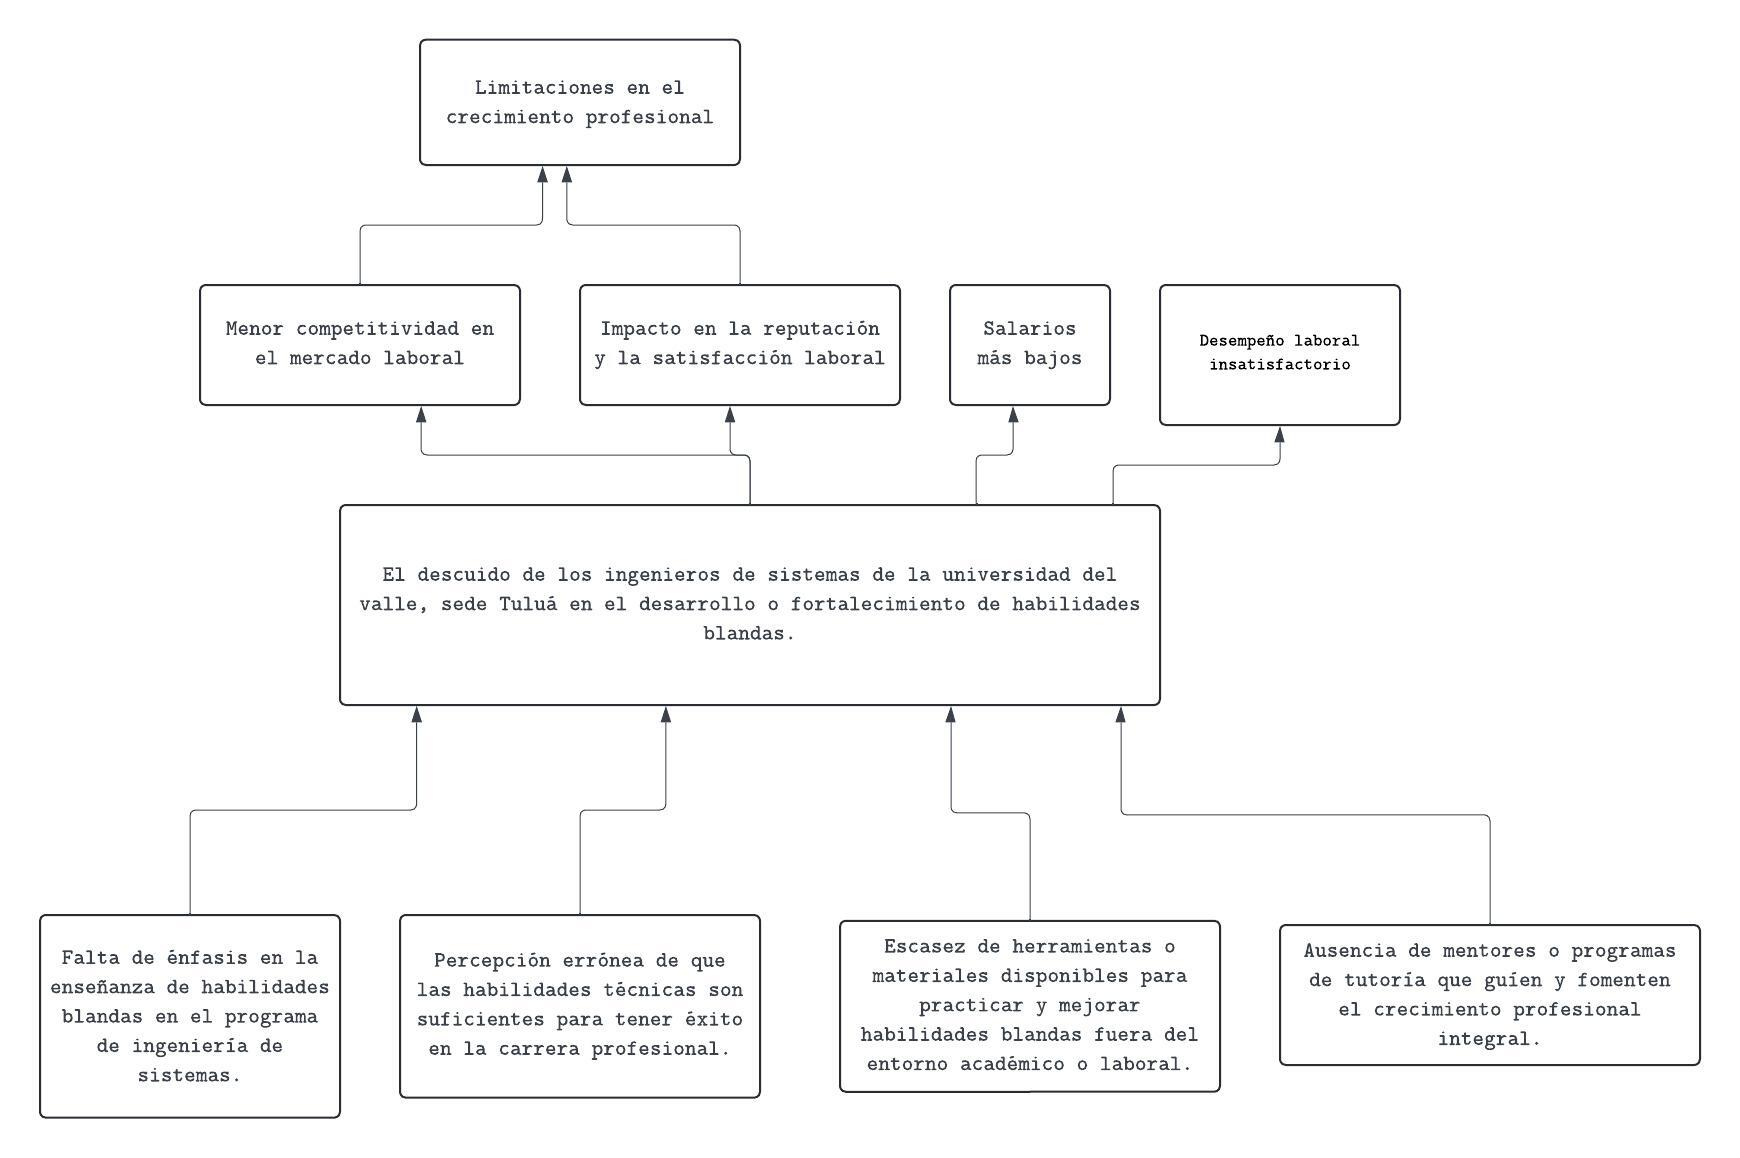
\includegraphics[width=\textwidth]{Figuras/Árbol de problemas.jpeg}
    \caption{Árbol de problemas. Elaboración propia.}
    \label{fig:problema_formulacion}
\end{figure}
\newpage
\section{Objetivos}

\subsection{Objetivo general}

Desarrollar los módulos de “aprender a aprender” y “escucha activa” empleando gamificación para el prototipo de plataforma enfocada en la enseñanza de habilidades blandas para los ingenieros de sistemas de la Universidad del Valle, sede Tuluá.

\subsection{Objetivos específicos}			

\begin{enumerate} [label=\arabic*, leftmargin=2.5em, itemsep=0.6\baselineskip]
    \item Identificar las teorías y enfoques clave relacionados con el aprendizaje autónomo y continuo, así como las estrategias efectivas para fortalecer la capacidad de aprender a aprender.
    \item Investigar metodologías y técnicas empleadas para fomentar la escucha activa durante las interacciones comunicativas, considerando la literatura académica y las mejores prácticas en el campo de la comunicación interpersonal.
    \item Desarrollar actividades gamificadas y experiencias de aprendizaje interactivas, utilizando recursos educativos relevantes que respalden el desarrollo de las habilidades blandas de 'Learning to learn' y 'Active listening'.
    \item Implementar los módulos de “aprender a aprender” y “escucha activa”.
    \item Evaluar la efectividad de los módulos en términos de comprensión del contenido, participación, motivación, retención de información y aplicación práctica, a través de pruebas piloto y retroalimentación de los estudiantes, identificando áreas de mejora.
\end{enumerate}

\section{Resultados esperados}
Para abordar la sección de resultados esperados, se puede consultar la tabla ~\ref{tab:resultados}, la cual se basa en los objetivos específicos. Al cumplir estos objetivos específicos, se logrará alcanzar el objetivo general.

\begingroup
\setlength{\tabcolsep}{10pt} % padding horizontal
\setlength{\extrarowheight}{3pt} 
\renewcommand{\arraystretch}{1.25}

\begin{longtable}{|p{8cm}|p{8cm}|}
\caption{Resultados esperados según los objetivos específicos}
\label{tab:resultados} \\
\hline
\textbf{Objetivo específico} & \textbf{Resultado esperado} \\
\hline
\endfirsthead

\hline
\textbf{Objetivo específico} & \textbf{Resultado esperado} \\
\hline
\endhead

\endfoot

\hline \hline
\endlastfoot

1. Identificar las teorías y enfoques clave relacionados con el aprendizaje autónomo y continuo, así como las estrategias efectivas para fortalecer la capacidad de aprender a aprender. 
& \begin{itemize}[leftmargin=*, topsep=0pt, partopsep=0pt, parsep=0pt, itemsep=0.4\baselineskip]
     \item Documento sobre los fundamentos teóricos y prácticos que sustenten el desarrollo del módulo “Learning to learn”
    \item Selección y adopción de las estrategias más adecuadas para fortalecer la capacidad de aprender a aprender de los estudiantes de ingeniería de sistemas de la Universidad del Valle, sede Tuluá.
\end{itemize}
\\ \hline

2. Investigar metodologías y técnicas empleadas para fomentar la escucha activa durante las interacciones comunicativas, considerando la literatura académica y las mejores prácticas en el campo de la comunicación interpersonal.
& \begin{itemize}[leftmargin=*, topsep=0pt, partopsep=0pt, parsep=0pt, itemsep=0.4\baselineskip]
     \item Documento sobre las diferentes técnicas y enfoques utilizados para fomentar la escucha activa.
    \item El diseño de actividades y estrategias en el módulo de “Active listening”
\end{itemize}
\\ \hline

3. Desarrollar actividades gamificadas y experiencias de aprendizaje interactivas, utilizando recursos educativos relevantes que respalden el desarrollo de las habilidades blandas de “aprender a aprender” y “escucha activa”. 
& \begin{itemize}[leftmargin=*, topsep=0pt, partopsep=0pt, parsep=0pt, itemsep=0.4\baselineskip]
     \item Conjunto de recursos educativos adaptados y seleccionados específicamente para respaldar el desarrollo de las habilidades blandas de “aprender a aprender” y “escucha activa”
    \item Conjunto de actividades gamificadas y experiencias de aprendizaje interactivas, que incluya instrucciones detalladas para cada actividad, así como materiales necesarios y pautas para la evaluación del aprendizaje y el progreso de los estudiantes. 
\end{itemize}
\\ \hline

4. Implementar los módulos de “aprender a aprender” y “escucha activa”. 
& \begin{itemize}[leftmargin=*, topsep=0pt, partopsep=0pt, parsep=0pt, itemsep=0.4\baselineskip]
    \item Diseños MER de la base de datos: Modelos Entidad-Relación (MER) detallados para la base de datos que soportará la aplicación.
    \item Integración de modelos de procesamiento de lenguaje natural (PLN): Implementación de modelos de OpenAI para la generación de contenidos personalizados, incluyendo roadmaps de aprendizaje adaptados al usuario en el módulo Aprender a Aprender, así como la creación dinámica de textos narrativos y diálogos para los desafíos del módulo de Escucha Activa, los cuales se integran con ElevenLabs para la síntesis y reproducción de audio.
    \item Documentación de la arquitectura de los módulos.
    \item El código fuente de los módulos.
\end{itemize}
\\ \hline

5. Evaluar la efectividad de los módulos en términos de comprensión del contenido, participación, motivación, retención de información y aplicación práctica, a través de pruebas piloto y retroalimentación de los estudiantes, identificando áreas de mejora.
& \begin{itemize}[leftmargin=*, topsep=0pt, partopsep=0pt, parsep=0pt, itemsep=0.4\baselineskip]
    \item Aplicación de encuestas de percepción de mejora a los usuarios que utilicen ambos módulos, con el propósito de evaluar su nivel de satisfacción, motivación y percepción de progreso en habilidades como la escucha activa y el aprendizaje autónomo.
    \item Un informe con el análisis y resultados de las pruebas realizadas, con conclusiones y recomendaciones para futuras mejoras.
\end{itemize}
\\ \hline

\end{longtable}
\section{Antecedentes}

Fortalecer las habilidades blandas en los ingenieros de sistemas en formación es fundamental para su desempeño y proyección en el entorno laboral. En coherencia con esta necesidad, diversas investigaciones y trabajos previos han identificado las competencias más relevantes, analizado su efecto en el desempeño laboral y propuesto lineamientos para su integración en la formación académica.

\subsection{A Systematic Mapping Study on Soft Skills in Software Engineering}

Desde un enfoque investigativo, la revista académica de Universal Computer Science, en su publicación \textbf{“A Systematic Mapping Study on Soft Skills in Software Engineering”}, escrita por Gerardo Matturo, Florencia Raschetti y Carina Fontán, informa sobre los resultados de un estudio de mapeo sistemático destinado a identificar el estado del arte sobre habilidades blandas en ingeniería de software y a determinar cuáles habilidades son relevantes para su práctica, basándose en la frecuencia con la que son mencionadas en la literatura revisada por los autores. Su objetivo es ayudar a los gerentes de Recursos Humanos y líderes de equipos de proyectos de software a conocer qué habilidades no técnicas son generalmente demandadas por la industria e identificar cuáles de ellas pueden ser adecuadas para su entorno \cite{Matturro2019}.

\subsection{Skills Development for Software Engineers: Systematic Literature Review}

De manera complementaria, en el artículo \textbf{“Skills development for software engineers: Systematic literature review”} se identifican las habilidades blandas necesarias para los futuros ingenieros de software y las metodologías de enseñanza que contribuyen a desarrollar tales habilidades desde el pregrado, manteniendo a los estudiantes motivados. Además, se propone un marco de trabajo para ayudar a los educadores a llevar a cabo un proceso de enseñanza-aprendizaje que incluya habilidades técnicas y blandas durante el pregrado de futuros ingenieros de software \cite{Borges2024}.

\subsection{Acquiring Professional Software Engineering Skills through Studio-based Learning}

La 17ª Conferencia Internacional sobre Educación Superior y Capacitación Basada en Tecnología de la Información (ITHET) 2018 presentó un estudio detallado sobre la implementación del aprendizaje basado en estudio (SBL) en el programa de Ingeniería de Software de la Universidad de Monmouth, titulado \textbf{“Acquiring Professional Software Engineering Skills through Studio-based Learning”} \cite{Rosca2018}. Esta implementación se centra en preparar a los estudiantes para ser contribuyentes exitosos en sus futuras empresas, inscribiéndolos en una experiencia SBL de dos semestres durante su último año. En este curso, los estudiantes trabajan en proyectos de software que simulan el ciclo de vida del desarrollo de software en un entorno real y practican actividades específicas de la industria que desarrollan habilidades profesionales clave, como el trabajo en equipo, la comunicación efectiva, el aprendizaje continuo y la capacidad de funcionar en equipos interdisciplinarios. El estudio no solo detalla cómo se ha llevado a cabo esta implementación, sino que también la compara con el marco definido por los investigadores de la Universidad de Lancaster. Una característica innovadora de este enfoque es que introduce un proceso de aprendizaje casi completamente dirigido por los estudiantes, con solo un marco de referencia para guiarlos, lo cual ha demostrado ser eficaz en el desarrollo de habilidades profesionales en los estudiantes.

\subsection{Soft Skills: The Software Developer's Life Manual}

En el ámbito editorial, el libro escrito por John Sonmez, titulado \textbf{“Soft Skills: The Software Developer’s Life Manual”}, es una guía práctica centrada en las habilidades blandas y en el bienestar general del desarrollador de software. Sonmez aborda una amplia gama de temas importantes, organizados en siete secciones: carrera y productividad, comercialización personal, aprendizaje y educación continua, habilidades de comunicación, finanzas personales, salud y estilo de vida y, por último, desarrollo personal. En cada sección brinda ejemplos de su propia experiencia y propone actividades para que los lectores puedan poner en práctica lo aprendido \cite{Sonmez2014}.

\subsection{Learning How to Learn: Aprendiendo a Aprender}

El curso \textbf{“Aprendiendo a aprender: Poderosas herramientas mentales con las que podrás dominar temas difíciles (Learning How to Learn)”} \cite{coursera2024} ofrece acceso a técnicas de aprendizaje invaluables utilizadas por expertos en diversas disciplinas, como arte, música, literatura, matemáticas, ciencia, deportes, y muchas más. Con estos enfoques, los estudiantes, independientemente de su nivel de habilidad en los temas que deseen dominar, pueden transformar su forma de pensar y su vida. Aquellos con experiencia avanzada obtienen una visión profunda de la maquinaria cerebral, con ideas para fomentar un nuevo y poderoso aprendizaje, consejos contraintuitivos para presentar exámenes y perspectivas para optimizar el tiempo dedicado a tareas y resolución de problemas. Aquellos que enfrentan dificultades descubren un conjunto de técnicas prácticas estructuradas para mejorar su desempeño.

\subsection{Desarrollo de una Herramienta de Apoyo para el Aprendizaje de Habilidades Blandas con Gamificación}

En el ámbito institucional, varios trabajos de grado desarrollados en la Universidad del Valle se articulan con la necesidad de fortalecer las habilidades blandas mediante propuestas tecnológicas y enfoques basados en gamificación. Entre ellos se encuentra el trabajo de Daniel Felipe Cossio Marulanda, titulado \textbf{“Desarrollo de una herramienta de apoyo para el aprendizaje de habilidades blandas con gamificación”} \cite{cossioMarulanda2024}, cuyo objetivo fue construir un prototipo o aplicación semilla orientada al desarrollo de habilidades blandas para el entorno laboral, con énfasis en el trabajo en equipo y el liderazgo. Este proyecto sirve como base para la implementación de diversos módulos que faciliten la práctica y adquisición de habilidades interpersonales a menudo pasadas por alto en la formación académica tradicional.

\subsection{Desarrollo de Módulos de Mindset y Fitness para Plataforma Gamificada}

Juan Camilo Azcárate Cárdenas, en su trabajo de grado \textbf{“Desarrollo de módulos de mindset y fitness para el prototipo de plataforma enfocada en la enseñanza de habilidades blandas mediante gamificación”} \cite{azcarateCardenas2024}, propone integrar dos nuevos módulos específicos: “Fitness”, orientado al bienestar general, y “Mindset”, destinado a transformar las reacciones ante la vida de reactivas a proactivas. Estos módulos buscan complementar y enriquecer la experiencia de aprendizaje de habilidades blandas para estudiantes y profesionales de ingeniería de sistemas.

\subsection{Creación de los Módulos de Productividad y Finanzas para Plataforma Gamificada}

El trabajo de grado de Daniel Gómez Suárez, titulado \textbf{“Creación de los módulos de productividad y finanzas para prototipo de plataforma web enfocada al aprendizaje de habilidades blandas”} \cite{gomezSuarez2024}, se centra en determinar la estrategia más adecuada para desarrollar e integrar los módulos de productividad y finanzas en la plataforma, orientada al fortalecimiento de habilidades blandas en estudiantes y profesionales de ingeniería de sistemas.

\subsection{Creación de Módulos Interactivos para el Desarrollo Continuo de la Oratoria y el Pensamiento Crítico}

El trabajo de grado titulado \textbf{“Creación de módulos interactivos para el Desarrollo Continuo de la Oratoria y el Pensamiento Crítico en el prototipo de enseñanza de habilidades blandas”}, desarrollado por Juan David Moreno Alfonso \cite{morenoAlfonso2025}, propone el diseño e implementación de dos módulos adicionales para la plataforma institucional orientada al fortalecimiento de habilidades blandas.
\\
\\
El proyecto se centra en las competencias de \textit{oratoria} y \textit{pensamiento crítico}, consideradas fundamentales para el desempeño académico y profesional. Para ello, el autor desarrolla módulos interactivos que permiten a los estudiantes practicar habilidades comunicativas y argumentativas mediante actividades guiadas, retroalimentación continua y ejercicios diseñados para simular escenarios reales de debate y exposición oral. 
\\
\\
El trabajo también documenta la arquitectura de software utilizada, el flujo de interacción entre pantallas, la infraestructura del sistema y la integración del backend y frontend necesarios para el funcionamiento de los módulos. Este proyecto constituye un antecedente relevante, pues amplía el alcance del prototipo institucional de habilidades blandas mediante nuevos componentes que fortalecen las capacidades comunicativas y cognitivas de los estudiantes, alineándose con los objetivos formativos de la Escuela de Ingeniería de Sistemas y Computación de la Universidad del Valle.



%%%%%%%%%%%%%%%%%%%%%%%%%%%%%%Capitulo 2%%%%%%%%%%%
\chapter{Alcance de la propuesta}
\markboth{Alcance de la propuesta}{Alcance de la propuesta}
\section{Declaración del alcance}
Este proyecto se centró en diseñar, desarrollar y poner en marcha los módulos Aprender a Aprender y Escucha Activa para el prototipo de plataforma gamificada orientada a la enseñanza de habilidades blandas. El trabajo estuvo dirigido específicamente a estudiantes de Ingeniería de Sistemas de la Universidad del Valle, sede Tuluá, con el propósito de fortalecer su capacidad de aprendizaje autónomo y promover prácticas de escucha activa mediante experiencias interactivas. Más allá del componente técnico, se buscó enfatizar la necesidad de integrar habilidades transversales dentro de la formación académica y profesional de ingeniería.
\\
\\
El desarrollo del proyecto enfrentó limitaciones asociadas tanto al tiempo como a la disponibilidad de recursos humanos, dado que su construcción fue realizada por una sola persona dentro de un periodo máximo de 12 meses. En consecuencia, el alcance se concentró en dos habilidades blandas específicaas (aprender a aprender y escucha activa) dejando fuera otros módulos potenciales. 
\\
\\
Esta investigación se basó en condiciones necesarias para garantizar su ejecución: el interés y la participación activa de los estudiantes en el uso de la plataforma, el acompañamiento docente durante todas las etapas del desarrollo, y el acceso a recursos institucionales adecuados para la revisión, prueba y seguimiento del proyecto. Estas condiciones humanas y organizacionales permitieron avanzar en el proceso de implementación y sentaron las bases para la validación del prototipo.
\\
\\
A partir de estas condiciones iniciales, la ejecución del proyecto también dependió de requisitos técnicos fundamentales para asegurar su éxito: el acceso continuo a servicios externos como modelos de procesamiento de lenguaje natural (PLN) y sintetizadores de voz; la disponibilidad de internet para probar la plataforma de manera constante; un entorno de desarrollo con los recursos necesarios para ejecutar e integrar los servicios basados en LLM; y la utilización de herramientas modernas de desarrollo web para construir tanto el frontend como el backend del prototipo. Estas condiciones resultaron esenciales para la implementación y el correcto funcionamiento de los módulos desarrollados, especialmente aquellos que requieren generación dinámica de contenido.
\\
\\
El alcance del proyecto incluyó los siguientes componentes principales:
\begin{enumerate}
    \item \textbf{Módulo de gestión del aprendizaje (Aprender a Aprender):}
    Este módulo integró herramientas para la planificación, organización y seguimiento del aprendizaje mediante la creación de metas, objetivos y tareas. Incluyó un tablero Kanban para la gestión visual de actividades y un sistema de autoevaluaciones que promueva la reflexión del estudiantes. 

    \item \textbf{Generación y edición de roadmaps de aprendizaje:}
    Se desarrolló un editor visual que permite a los usuarios construir, organizar y ajustar rutas de aprendizajes personalizadas. Este componente incorporó un agente conversacional basado en modelos de procesamiento de lenguaje natural (PLN), capaz de generar roadmaps adaptados a las necesidades e intereses del estudiante, facilitando la orientación inicial del proceso de aprendizaje.

    \item \textbf{Integración bidireccional entre roadmaps y planificación del aprendizaje:}
    La plataforma permitió transformar la estructura de metas, objetivos y tareas en un roadmap visual que podía hacerse público para compartir distintas formas de abordar un proceso de aprendizaje. A su vez, los roadmpas existentes podían convertirse nuevamente en metas, objetivos y tareas, de modo que cada usuario pudiera adoptar o adaptar rutas creadas por otros según sus necesidades.

    \item \textbf{Módulo de entrenamiento en escucha activa (gamificado):}
    Este módulo ofreció una experiencia interactiva compuesta por sesiones de juego divididas en rondas dinámicas. Cada ronda presentó desafíos auditivos generados mediante inteligencia artificial, con diferentes modos de juego (selección múltiple, completar espacios, parafraseo, resumen y formulación de preguntas de clarificación). El sistema evaluó automáticamente las respuestas y ofreció retroalimentación inmediata para fortalecer la comprensión auditiva y la atención activa.

    \item \textbf{Generación y reproducción de audio con modelos de IA:}
    Los desafíos del módulo de escucha activa integraron síntesis de voz mediante servicios externos, lo que permitió obtener audios con distintos estilos, voces y niveles de dificultad. El sistema gestionó la creación, almacenamiento y reproducción de estos recursos para garantizar la disponibilidad del contenido auditivo requerido en cada ronda de juego.
\end{enumerate}

%%%%%%%%%%%%%%%%%%%%%%%%%%%%%%Capitulo 3%%%%%%%%%%%
\chapter{Marco de referencia}
\markboth{Marco de referencia}{Marco de referencia}
\section{Marco teórico}

\subsection{Habilidades blandas: fundamentos teóricos}

\begin{itemize}
    \item \textbf{Competencias:} De acuerdo con el Ministerio de Educación Nacional, es el “conjunto de conocimientos, actitudes, disposiciones y habilidades (cognitivas, socioafectivas y comunicativas), relacionadas entre sí para facilitar el desempeño flexible y con sentido de una actividad en contextos relativamente nuevos y retadores. Por lo tanto, la competencia implica conocer, ser y saber hacer” \cite{Ministerio2024}.
    
    \item \textbf{Habilidades blandas:} Las habilidades blandas son competencias no técnicas que facilitan un desempeño eficaz en contextos sociales y laborales diversos. A diferencia de las habilidades técnicas, las habilidades blandas no dependen de la interacción con máquinas y son aplicables en una variedad de contextos profesionales, implican capacidades interpersonales e intrapersonales. Se consideran componentes subyacentes de la competencia de un individuo y están relacionadas con su motivación, rasgos de personalidad y conocimiento \cite{Marin-Zapata2022}.
\end{itemize}

\subsection{Teorías del aprendizaje}
Las teorías del aprendizaje son útiles para comprender cómo se adquieren y se modifican conocimientos, creencias, conductas, actitudes, habilidades y destrezas. 
\\
\\
A continuación, se presentan las teorías del aprendizaje seleccionadas por su relevancia y aplicabilidad al diseño de los módulos implementados en este proyecto.

\subsubsection{Aprendizaje autorregulado}
El aprendizaje autorregulado (Self-Regulated Learning, SRL) es una perspectiva teórica que explica cómo los estudiantes gestionan de manera activa y deliberada sus propios procesos cognitivos, motivacionales y conductales para alcanzar metas de aprendizaje. Este modelo ha sido desarrollado principalmente por Barry J. Zimmerman, quien lo define como “el proceso autodirigdo mediante el cual los estudiantes transforman sus habilidades mentales en habilidades académicas” \cite{Zimmerman2002}. Esta perspectiva señala que aprender no consiste únicamente en poseer ciertas capacidades cognitivas, si no en saber cómo organizar, monitorear, regular y evalur el propio desempeño durante una tarea académica.
\\
\\
Zimmerman señala que los aprendices autorregulados se caracterizan por adoptar un rol activo en su formación: identifican sus fortalezas y limitaciones, establecen metas claras, seleccionan estrategias aadecuadas, supervisan su ejecución y ajustan su comportamiento en función de los resultados obtenidos. De acuerdo con el autor “el aprendizaje es una actividad que los estudiantes realizan por sí mismos de manera proactiva, y no un evento pasivo que ocurre como reacción a la enseñanza” \cite{Zimmerman2002}.
\\
\\
El modelo de aprendizaje autorregulado se organiza en tres fases cíclicas, las cuales interactúan entre sí y permiten que el estudiante mejore progresivamente su capacidad de aprender de manera autónoma:

\paragraph{1. Fase de premeditación (forethought)}

Esta fase ocurre antes de iniciar una tarea e involucra procesos de análisis y preparación:

\begin{itemize}
    \item \textbf{Análisis de la tarea:} Incluye el establecimiento de metas específicas y la planificación estratégica. Zimmerman destaca que los estudiantes que fijan metas cercanas y bien definidas suelen mostrar mayores niveles de autoeficacia y persistencia.
    
    \item \textbf{Creencias motivacionales:} Comprende la autoeficacia, las expectativas de resultado, el interés intrínseco y la orientación hacia el aprendizaje. Estas creencias influyen directamente en la disposición con la que el estudiante enfrenta la actividad.
\end{itemize}

\paragraph{2. Fase de desempeño (performance)}

Corresponde a los procesos que ocurren durante la ejecución de la tarea:

\begin{itemize}
    \item \textbf{Autocontrol:} Implica el uso de estrategias cognitivas, metacognitivas y conductuales, tales como la autoinstrucción, la organización del entorno de estudio y la regulación de la atención.
    
    \item \textbf{Autoobservación:} Se refiere al monitoreo continuo del propio desempeño, el registro de avances y la identificación de errores. Zimmerman sostiene que incluso prácticas simples de auto-monitoreo pueden generar mejoras espontáneas en el rendimiento académico.
\end{itemize}

\paragraph{3. Fase de autorreflexión (self-reflection)}

Incluye los procesos posteriores a la ejecución de la tarea:

\begin{itemize}
    \item \textbf{Juicio personal:} Consiste en comparar los resultados obtenidos con las metas previamente establecidas, así como en analizar las causas del éxito o fracaso.
    
    \item \textbf{Reacciones adaptativas o defensivas:} Implica ajustar estrategias, modificar creencias o tomar decisiones para futuras tareas. Atribuciones causales centradas en factores controlables, como el uso de estrategias, fortalecen la motivación; en contraste, atribuciones basadas en la falta de capacidad suelen conducir a la desmotivación.
\end{itemize}

Zimmerman plantea que estas fases se articulan como un ciclo continuo, ya que la reflexión y evaluación de una experiencia influyen directamente en la planificación de la siguiente. De este modo, el aprendizaje autorregulado se concibe como un proceso dinámico y progresivo, que puede mejorar gradualmente a través de la enseñanza y la práctica continua.

\subsubsection{Metacognición}
La metacognición es el conjunto de conocimientos y experiencias que las personas poseen sobre sus propios procesos cognitivos, así como la capacidad de supervisarlos, regularlos y controlarlos durante actividades intelectuales. Este concepto fue introducido formalmente por John H. Flavell en su obra \textbf{“Metacognition and Cognitive Monitoring”} \cite{Flavell1979}, donde indica que estos procesos resultan esenciales en tareas como la comprensión, la memoria, la comunicación, la resolución de problemas y distintas formas de autocontrol cognitivo.
\\
\\
Flavell explica que el monitoreo cognitivo está constituido de cuatro elementos centrales \cite{Flavell1979}: El conocimiento metacognitivo, las experiencias metacognitivas, las metas o tareas y las acciones o estrategias. Estos componentes operan de manera articulada para permitir que las personas regulen de forma efectiva su pensamiento y aprendizaje.

\paragraph{1. Conocimiento metacognitivo}

Es el conjunto de creencias y saberes que una persona posee acerca de sí misma y de los demás como aprendices, de las características de las tareas cognitivas y de las estrategias que pueden utilizarse para afrontarlas. Flavell organiza este conocimiento en tres categorías:

\begin{itemize}
    \item \textbf{Persona:} incluye creencias sobre uno mismo y sobre otros como agentes cognitivos, considerando diferencias individuales y propiedades universales del funcionamiento mental.
    \item \textbf{Tarea:} comprende el entendimiento de las características de una actividad (dificultad, familiaridad, estructura) y de cómo estas influyen en el desempeño.
    \item \textbf{Estrategia:} alude al conocimiento de los procedimientos cognitivos o metacognitivos disponibles, así como su eficacia en distintos contextos.
\end{itemize}

Flavell señala que este conocimiento puede activarse de forma consciente o automática y no siempre es exacto, lo cual afecta la calidad del monitoreo cognitivo.

\paragraph{2. Experiencias metacognitivas:}
Son los estados cognitivos y afectivos que surgen antes, durante o después de una tarea intelectual. Pueden manifestarse como dudas, sensaciones de comprensión o falta de ella, percepciones de progreso o dificultad, o sentimientos de seguridad respecto a la ejecución.
\\
\\
Estas experiencias cumplen tres funciones principales:

\begin{itemize}
    \item \textbf{Ajustar metas o tareas:} por ejemplo, volver a leer un texto al percibir falta de comprensión.
    \item \textbf{Modificar el conocimiento metacognitivo:} actualizar creencias o corregir percepciones previas.
    \item \textbf{Activar estrategias cognitivas o metacognitivas:} como autoevaluar la comprensión o repetir información difícil.
\end{itemize}

\paragraph{3. Metas o tareas}

Se refieren a los objetivos que guían la actividad cognitiva. Según Flavell, la naturaleza de la meta (su claridad, dificultad o relevancia) determina qué estrategias son necesarias y qué grado de monitoreo se debe aplicar para completarla con éxito.

\paragraph{4. Acciones o estrategias}

Son los procedimientos utilizados para alcanzar metas cognitivas o metacognitivas. Flavell distingue entre:

\begin{itemize}
    \item \textbf{Estrategias cognitivas:} orientadas a mejorar el desempeño directo en una tarea (por ejemplo, releer para memorizar).
    \item \textbf{Estrategias metacognitivas:} orientadas a evaluar o regular el propio desempeño (por ejemplo, autoformular preguntas para comprobar comprensión).
\end{itemize}


\subsubsection{Teoría del constructivismo}
La teoría del constructivismo, atribuida a Jean Piaget, sostiene que el aprendizaje es un proceso activo en el que los individuos construyen su propio conocimiento a través de la interacción con el entorno y la reinterpretación de sus experiencias. De tal forma, se reconoce que cada persona es responsable de elaborar su comprensión del mundo a partir de sus experiencias previas, conocimientos previos y percepciones individuales.
\\
\\
El conocimiento es una construcción del ser humano: cada persona percibe la realidad, la organiza y le da sentido en forma de constructos, lo que contribuye a la edificación de un todo coherente que da sentido y unicidad a la realidad \cite{OrtizGranja2015}. Por lo tanto, al ser el individuo un participante activo en su propio proceso de aprendizaje es crucial fomentar la autonomía, recordando la importancia de aprender por cuenta propia.

\subsubsection{Teoría del aprendizaje social}
La teoría del aprendizaje social de Albert Bandura refuerza la idea de que el aprendizaje es el resultado de la observación al entorno social y la imitación. En su libro Social Learning Theory (1977) menciona: “Afortunadamente, en la mayoría de los humanos el comportamiento se aprende de manera observacional a través del modelado: al observar a otros se forma una idea de cómo se realizan los nuevos comportamientos, y en ocasiones posteriores, esta información codificada sirve como guía para la acción” \cite{Bandura1977}.
\\
\\
En su investigación, Bandura describe el aprendizaje social en cuatro principios: El primero indica que para aprender, es necesario prestar atención y estar enfocado; el segundo señala que la información recién adquirida debe ser internalizada y almacenada como recuerdo; el tercero implica la reproducción de la información retenida; y finalmente, el cuarto principio destaca la importancia de tener motivación, el cual es originado al observar las consecuencias, ya sean recompensas o castigos, que otros experimentan por sus acciones o decisiones.

\subsubsection{Teoría del aprendizaje experiencial}
La teoría del aprendizaje experiencial de David Kolb se cimenta en desarrollos y trabajos teóricos previos de autores como Jean Piaget, John Dewey y Kurt Lewin. Esta teoría establece la importancia de la experiencia en el proceso de aprendizaje. El desarrollo de David Kolb explora los procesos cognitivos asociados al abordaje y procesamiento de las experiencias y describe los diferentes estilos individuales de aprendizaje \cite{GomezPawelek2011}.
\\
\\
Kolb, propone seguir un proceso de cuatro etapas denominado “Ciclo de Kolb” para que exista un aprendizaje efectivo. Este ciclo empieza con la experiencia concreta, que se adquiere al hacer algo, luego se lleva a cabo la reflexión sobre los resultados obtenidos (etapa de observación reflexiva), después se extraen conclusiones o generalizaciones (etapa de conceptualización abstracta) a partir de la experiencia y por último, se pone en práctica las conclusiones formuladas para orientar nuestras acciones en situaciones futuras (etapa de experimentación activa).

\subsubsection{Teoría del aprendizaje significativo}
De acuerdo con el psicólogo educativo David Ausubel, el aprendizaje significativo se da cuando una nueva información es integrada y comprendida en función de un conocimiento anterior, en lugar de ser memorizada de manera aislada. Se produce así una interacción entre los nuevos contenidos y los elementos relevantes ya presentes en la estructura cognitiva. La presencia de ideas, conceptos o proposiciones inclusivas, claras y disponibles en la mente del aprendiz es lo que dota de significado al nuevo aprendizaje \cite{PalmeroRodriguez2024}.

\subsubsection{Teoría del aprendizaje por descubrimiento}
Jerome S. Bruner, plantea la importancia del descubrimiento personal en el aprendizaje, para que sea significativo. Según Bruner, el individuo adquiere conocimiento cuando es descubierto por sí mismo o por su propio discernimiento, ya que involucra la exploración activa, la experimentación y la resolución de problemas por parte de éste. Así mismo, con este tipo de aprendizaje es más probable que la información sea conservada.
\\
\\
Para que se produzca un aprendizaje por descubrimiento, es indispensable que se planteen objetivos específicos que guíen la investigación del individuo.  Estos objetivos actúan como puntos de referencia que orientan el proceso de descubrimiento y facilitan la consecución de resultados concretos. Además, es fundamental que exista una familiarización con las herramientas utilizadas para el descubrimiento de información, ya que estas proporcionan los medios necesarios para llevar a cabo cualquier investigación de manera efectiva. 
\\
\\
Por último, Bruner sugiere que el tanto investigar como experimentar propicia la fijación de conocimientos y es la manera más natural de adquirir competencias. También ayuda a la motivación del aprendiz, a fomentar el uso de la creatividad en la resolución de problemas, a estimular la intuición e impulsa el aprender a aprender. 

\subsection{Procesamiento del Lenguaje Natural (PLN)}
El Procesamiento del Lenguaje Natural (PLN) es una rama de la inteligencia artificial que estudia cómo los sistemas computacionales pueden representar, comprender, analizar y generar lenguaje humano, tanto en su forma escrita como hablada. Según lo planteado por Jurafky y Martin en “Speech and Language Processing” \cite{JurafskyMartin2023}, el PLN integra principios de la lingüística, modelos matemáticos, técnicas de aprendizaje automático e ingeniería de sistemas para procesar grandes volúmenes de información lingüística, modelar su estructura y significado, así como interpretar su uso en distintos contextos comunicativos.

\subsubsection{Modelos de lenguaje de gran escala (Large Language Models, LLM)}

Los modelos de lenguaje de gran escala (Large Language Models, LLM) constituyen una rama emergente dentro del procesamiento del lenguaje natural, caracterizada por arquitecturas profundas basadas en transformadores que contienen decenas de miles de millones de parámetros y que han sido entrenadas en vastos corpus textuales. Según el recurso de Elastic, un LLM es “un modelo entrenado con algoritmos de aprendizaje profundo capaz de realizar una amplia gama de tareas de procesamiento de lenguaje natural” \cite{ElasticLLM}.
\\
\\
El funcionamiento básico de estos modelos implica tres etapas fundamentales:
\begin{itemize}
  \item \textbf{Pre-entrenamiento:} el modelo es entrenado sin supervisión en grandes cantidades de datos lingüísticos, lo que le permite inferir patrones estadísticos del lenguaje \cite{ElasticLLM}.
  \item \textbf{Ajuste fino (fine-tuning):} para tareas específicas, el modelo se adapta con datos etiquetados o ejemplos, mejorando su rendimiento en dominios particulares \cite{ElasticLLM}.
  \item \textbf{Prompt-tuning o aprendizaje en contexto (few-shot/zero-shot):} el modelo es guiado mediante instrucciones o ejemplos mínimos para realizar nuevas tareas sin entrenamiento adicional extenso \cite{ElasticLLM}.
\end{itemize}

Además, los LLM suelen emplear tres componentes técnicos principales: capas de embedding para representar palabras o tokens en vectores, mecanismos de atención para detectar dependencias de largo alcance y capas feed-forward que procesan la información codificada. \cite{ElasticLLM}.
\\
\\
Estos modelos han sido aplicados con éxito en múltiples ámbitos: generación de texto, chatbots conversacionales, generación de código, análisis de sentimientos, motores de búsqueda mejorados y sistemas de recomendación. No obstante, también enfrentan desafíos significativos como las alucinaciones, los sesgos, los riesgos de privacidad y los altos requerimientos computacionales \cite{ElasticLLM}.
\\
\\
Dentro del contexto de este proyecto, los LLM constituyen un fundamento tecnológico para la generación automática de retroalimentación, la interpretación del lenguaje de los usuarios, la producción de contenido educativo personalizado y el soporte de agentes conversacionales inteligentes que intervienen en los módulos diseñados.


\subsection{Teoría general de sistemas}

La teoría general de los sistemas (TGS), propuesta por Ludwig Von Bertalanffy, ampliamente aplicada en diversos campos de conocimiento, es definida como el estudio interdisciplinario de los sistemas y sus interrelaciones dentro de sistemas más complejos. Una premisa fundamental de esta teoría es: “el todo es más que la suma de las partes” (Aristóteles), es decir, al examinar de manera holística la interacción entre diferentes componentes de un sistema, pueden surgir características de éste que no son evidentes si se observarán cada una de sus partes de forma independiente.
\\
\\
La TGS se distingue por su perspectiva integradora, donde se considera importante la interacción y los conjuntos que a partir de ella se generan, ofreciendo un ambiente adecuado para la interrelación y comunicación entre especialistas. Con ello, contradice la mirada fragmentaria y lineal del enfoque reduccionista, método con el cual los fenómenos se estudian de una forma independiente como si fueran una realidad dividida \cite{GutierrezGomez2013}.

\subsection{Principios de diseño y usabilidad}

La usabilidad es un aspecto central en el diseño de sistemas interactivos y se refiere al grado en que un producto permite a los usuarios alcanzar objetivos específicos con eficacia, eficiencia y satisfacción. Nielsen, establece que la usabilidad no es un rasgo único o unidimensional, sino un concepto compuesto por cinco dimensiones que permiten evaluar de forma integral la experiencia del usuario: \textit{aprendibilidad}, \textit{eficiencia}, \textit{memorabilidad}, \textit{errores} y \textit{satisfacción}. Estas dimensiones describen, respectivamente, qué tan fácil resulta para un usuario aprender a usar un sistema, qué tan rápido puede ejecutar tareas, cómo recuerda su funcionamiento tras un periodo de no uso, qué tan propenso es a cometer errores y qué tan satisfecho se siente con la experiencia.
\\
\\
\textbf{Heurísticas de usabilidad de Nielsen.}  
Nielsen propone diez heurísticas que funcionan como principios generales para el diseño de interfaces centradas en el usuario \cite{NielsenMolich1990}. Estas heurísticas son ampliamente utilizadas en ingeniería de usabilidad y diseño de experiencias digitales:

\begin{enumerate}
    \item \textbf{Visibilidad del estado del sistema.} 
    El sistema debe mantener informados a los usuarios sobre lo que está ocurriendo, proporcionando retroalimentación oportuna y comprensible.

    \item \textbf{Correspondencia entre el sistema y el mundo real.}
    La interfaz debe emplear conceptos, terminología y convenciones familiares para los usuarios, siguiendo el orden lógico y natural propio del mundo real.

    \item \textbf{Control y libertad del usuario.}
    El sistema debe permitir que los usuarios deshagan y rehagan acciones fácilmente, así como navegar o salir de estados no deseados sin dificultad.

    \item \textbf{Consistencia y estándares.}
    La interfaz debe mantener coherencia en su diseño y seguir convenciones establecidas, evitando que el usuario tenga que adivinar si diferentes elementos realizan acciones similares.

    \item \textbf{Prevención de errores.}
    El diseño debe anticipar y minimizar la aparición de errores, ya sea restringiendo entradas no válidas o proporcionando mecanismos que reduzcan la posibilidad de equivocación.

    \item \textbf{Reconocimiento antes que recordación.}
    El sistema debe reducir la carga de memoria del usuario al mostrar opciones, elementos y acciones relevantes, evitando que dependa de recordar información entre distintas partes de la interfaz.

    \item \textbf{Flexibilidad y eficiencia de uso.}
    La interfaz debe ser usable tanto para usuarios novatos como expertos, incorporando atajos, personalización u otros mecanismos que permitan acelerar tareas frecuentes.

    \item \textbf{Diseño estético y minimalista.}
    El contenido presentado debe ser claro y esencial, evitando información irrelevante o excesiva que pueda distraer o sobrecargar cognitivamente al usuario.

    \item \textbf{Ayuda a los usuarios a reconocer, diagnosticar y recuperarse de errores.}
    Los mensajes de error deben expresarse en lenguaje claro, indicando el problema, su causa y posibles soluciones concretas para recuperarse.

    \item \textbf{Ayuda y documentación.}
    Aunque lo ideal es que el sistema sea intuitivo, debe ofrecer documentación accesible, fácil de buscar y enfocada en describir pasos concretos para completar tareas.
\end{enumerate}

Estas heurísticas constituyen una guía práctica para evaluar y mejorar interfaces, y son aplicables tanto en sistemas web como en aplicaciones móviles, plataformas educativas o herramientas basadas en inteligencia artificial.
\\
\\
\textbf{Principios de diseño centrado en el usuario:}  
Norman, en \textit{The Design of Everyday Things} \cite{Norman2013}, destaca que el diseño centrado en el usuario se fundamenta en la comprensión profunda de las necesidades, objetivos y limitaciones de los usuarios. Dentro de este enfoque se resaltan cuatro principios clave:

\begin{itemize}
    \item \textbf{Comprensión de los usuarios:} análisis de necesidades, contexto, limitaciones y comportamientos.
    \item \textbf{Diseño iterativo:} ciclos de prototipado, evaluación y refinamiento progresivo.
    \item \textbf{Evaluación continua:} pruebas con usuarios durante todas las fases del desarrollo.
    \item \textbf{Diseño inclusivo:} consideración de diversidad de usuarios, capacidades y contextos.
\end{itemize}

El enfoque centrado en el usuario es especialmente relevante para sistemas educativos y herramientas basadas en inteligencia artificial, donde la facilidad de uso y la claridad de las interacciones influyen directamente en la experiencia y el aprendizaje del usuario.

\section{Estado del arte}

Históricamente filósofos, psicólogos, sociólogos y pedagogos, han resaltado la importancia de las competencias transversales y socioemocionales (CTSE) en la educación de los individuos, que debe abarcar múltiples dimensiones, incluyendo el desarrollo cognitivo y el socioemocional. Las habilidades “blandas” o “no cognitivas” son rasgos de la personalidad de un individuo que no dependen de conocimientos técnicos previos y que le permite interactuar, comunicarse y trabajar con otros.
\\
\\
La Corporación Andina de Fomento (CAF), el Banco Mundial, el Banco Interamericano de Desarrollo (BID) y la Organización de Cooperación y Desarrollo Económico (OCDE) han sido actores importantes en la promoción y discusiones políticas contemporáneas en torno al fomento de las CTSE. La publicación del reporte “Desconectados” del BID en 2012 aporta una perspectiva muy pertinente a la discusión sobre la calidad de la educación en América Latina, indicando la existencia de un desacople entre las habilidades que se forman actualmente en el sistema educativo y las que son requeridas en el mercado laboral. De igual forma, el reporte de “Más Habilidades para el Trabajo y la Vida” de la CAF en 2016 señala que América Latina necesita incrementar sus esfuerzos en desarrollar en los jóvenes un conjunto de habilidades que les permita navegar y adaptarse a los entornos cambiantes de los próximos años.
\\
\\
La evidencia a nivel internacional basada principalmente en estudios empíricos y longitudinales en países desarrollados destaca la relevancia de las competencias transversales y socioemocionales (CTSE) en el proceso de aprendizaje y en los logros tanto actuales como futuros de los individuos. Por ejemplo, se ha observado una correlación positiva entre estas competencias y la finalización de estudios universitarios, el nivel de ingresos, el bienestar físico y mental, así como con el bienestar subjetivo, entre otros aspectos \cite{Huerta2019}. 
\\
\\
No existe consenso aún frente a cómo nombrar las habilidades blandas y una definición única y universal, dado a que cada entidad o institución tiende a enfocarse en aspectos específicos dentro de este amplio espectro de competencias. Este desafío se evidencia en la diversidad de enfoques y terminología utilizada por diferentes estudios, organizaciones y sectores. Mientras algunas pueden referirse a estas habilidades como competencias transversales y socioemocionales, otras pueden preferir términos como habilidades interpersonales, habilidades para la vida o habilidades no cognitivas \cite{RomeroGonzalez2021}.
\\
\\
Las habilidades blandas contemplan, entre otras, la capacidad de comunicarse, trabajar en equipo, empatía, adaptabilidad, resiliencia, autogestión, proactividad, autocrítica, honestidad, pensamiento analítico e innovación, aprendizaje activo y estrategias de aprendizaje, creatividad, originalidad e iniciativa, pensamiento crítico, liderazgo e influencia social, inteligencia emocional, razonamiento y resolución de problemas. Estas contribuyen al crecimiento personal y profesional del estudiante, así como a su convivencia entre pares y la comunicación efectiva dentro y fuera de una organización \cite{CepedaGuerra2021}. 
\\
\\
En un contexto donde la tecnología avanza y se reinventa rápidamente, el entorno se torna cada vez más competitivo. Adecco \cite{Adecco2024}, la empresa consultora en recursos humanos y de procesos de selección de personal, expone que quiénes desarrollan sus habilidades blandas, son los que obtienen ventaja competitiva frente a los cambios del entorno, ya que la demanda del mercado está apostando por los candidatos que demuestren estas habilidades, incluso las empresas están invirtiendo en programas de desarrollo que fortalezcan estos atributos en sus empleados. 
\\
\\
En el trabajo de grado de “Habilidades blandas y su influencia en el clima laboral de las organizaciones: una mirada actual para Colombia”, se aborda la creciente importancia de las habilidades blandas en el contexto laboral contemporáneo y como influyen de algún modo en el clima laboral de las organizaciones, puesto que contribuyen a la sostenibilidad y productividad de estas. Las empresas buscan ser competitivas no solo con personal técnicamente preparado, sino también con líderes y equipos de trabajo eficaces, eficientes y comprometidos \cite{PerdomoRamos2023}.
\\
\\
Es crucial que las instituciones educativas sean capaces de adaptarse y proporcionar a sus estudiantes alternativas para que adquieran las habilidades necesarias y se conviertan en profesionales altamente cualificados en sus respectivos campos. En la actualidad quiénes responden estas demandas, lo hacen con plataformas tecnológicas de enseñanza y aprendizaje que sirven de complemento al modelo tradicional de aula. 
\\
\\
En el artículo “Praxis sobre el desarrollo de competencias blandas en estudiantes de educación superior en aulas virtuales”, realizan una revisión bibliográfica sobre el desarrollo de competencias blandas en ambientes virtuales de enseñanza superior, comprobando así que las instituciones que se están adaptando a estas necesidades desarrollando plataformas y estrategias, monitorean constantemente el desarrollo de competencias de los estudiantes, evaluando sus avances y estableciendo un plan de mejora continua conforme a objetivos planteados y de la retroalimentación de los estudiantes \cite{CepedaGuerra2021}.
\\
\\
En la investigación “Soft skills in software engineering in higher education. An initial study of its state in Latin America”, se mencionan diversos autores que han discutido sobre la necesidad y relevancia de incorporar en los currículos de los programas de estudio de ingeniería de sistemas la enseñanza o la visibilización sobre habilidades blandas. Plantean que en la actualidad los estudiantes no solo deben desarrollar competencias técnicas, sino también competencias transversales para que realicen actividades profesionales de manera efectiva en un mundo globalizado, sin embargo, son el eslabón perdido en la ingeniería de sistemas, ya que los planes de estudios suelen marginar estas habilidades.
\\
\\
Adicionalmente, en el artículo de investigación anteriormente mencionado, se presentan los resultados de una encuesta realizada a directores, coordinadores y responsables académicos de 115 programas universitarios de ingeniería de sistemas en 85 universidades de 15 países de América Latina sobre el estado actual de la enseñanza de habilidades blandas en estas carreras. Casi la mitad de los programas encuestados incluyen cursos específicos sobre estas habilidades, como comunicación, trabajo en equipo, liderazgo, ética profesional y gestión de conflictos. Sin embargo, hay otras habilidades consideradas relevantes para la ingeniería de software que no se mencionaron, como habilidades de presentación, negociación, resolución de problemas, interés por aprender y autonomía.
\section{Marco conceptual}

\begin{itemize}

\item \textbf{Aprender a aprender:} En el 2006, el parlamento europeo y el Consejo de Educación definieron aprender a aprender como la capacidad de perseguir y persistir en el aprendizaje, organizar el propio aprendizaje, incluyendo la gestión efectiva del tiempo y la información, tanto de manera individual como en grupo. Esta competencia abarca el reconocimiento del propio proceso de aprendizaje y sus necesidades, identificar las oportunidades disponibles y la capacidad de superar obstáculos para aprender con éxito. Implica adquirir, procesar y asimilar nuevos conocimientos y habilidades, así como buscar y utilizar orientación \cite{GarciaVazquez2015}.
\\
\\
Aprender a aprender motiva a los individuos a basarse en aprendizajes previos y experiencias de vida para aplicar conocimientos y habilidades en diversos contextos, ya sea en el hogar, en el trabajo, en la educación o la formación. La motivación y la confianza son elementos esenciales para esta competencia.

\item \textbf{Aprendizaje activo:} Se fundamenta en la teoría del Constructivismo, la cual destaca que los alumnos construyen su propio conocimiento. Este enfoque de enseñanza implica que los estudiantes participen activamente en el proceso de aprendizaje, desarrollando su conocimiento y comprensión a través de oportunidades de aprendizaje diseñadas por sus docentes \cite{cambridge2024}.

\item \textbf{Escucha activa:} El término “escucha activa” fue introducido en 1957 por Carl Rogers y Richard Farson. También puede ser referido como escucha reflexiva. Es una habilidad de comunicación que implica no limitarse a solo escuchar las palabras que otra persona dice, si no escuchar con la intención de entender completamente a la otra persona.
\\
\\
La escucha activa es la práctica de prepararse para escuchar, observar los mensajes verbales y no verbales que se están enviando, y luego proporcionar retroalimentación apropiada con el fin de mostrar atención al mensaje que se está presentando \cite{UNIR2024}.

\item \textbf{Gamificación:} Aplicación de estrategias y mecánicas de juegos en contextos no jugables, con el fin de identificar aspectos susceptibles de ser convertidos en juegos o dinámicas lúdicas dentro de una actividad, tarea o mensaje determinado en un entorno de NO-juego. El objetivo es crear una experiencia significativa y motivadora que incentive un cambio de comportamiento, transmita un mensaje o contenido, y promueva una vinculación especial con los usuarios. En resumen, gamificar implica aplicar pensamientos y técnicas de juego para que las personas adopten ciertos comportamientos en contextos no relacionados con los juegos \cite{jenui2014}.

\item \textbf{Experiencia de usuario (UX):} La Experiencia de Usuario (UX) se centra en la percepción y sensaciones que experimenta una persona al interactuar con un producto, servicio o plataforma digital. Esta experiencia engloba todos los elementos de interacción, desde la forma en que se navega y se visualiza, hasta la facilidad con la que se utiliza y la satisfacción que genera en el usuario. En resumen, se trata de la impresión general y el nivel de comodidad que un usuario experimenta al utilizar un sitio web, una aplicación móvil u otro producto digital. Además, la UX no solo se limita a la utilidad y la estética, sino que también se preocupa por la emoción y el impacto emocional que deja en el usuario durante y después de la interacción.

\item \textbf{Plataformas de e-learning:} Una plataforma de e-learning es un entorno virtual diseñado para facilitar la administración y el acceso a una variedad de recursos educativos en línea. Estos recursos incluyen cursos completos, materiales multimedia, herramientas de comunicación interactivas, evaluaciones y la capacidad de monitorear el progreso del estudiante a lo largo del tiempo. Además de proporcionar contenido educativo, estas plataformas suelen ofrecer funciones adicionales como foros de discusión, chats en tiempo real, y la posibilidad de realizar trabajos colaborativos. 
\\
\\
Las plataformas de e-learning brindan una experiencia integral de aprendizaje en línea, permitiendo a los estudiantes aprender de manera flexible y a los educadores gestionar eficazmente el proceso educativo.

\item \textbf{Retroalimentación:} La retroalimentación es un proceso mediante el cual se proporciona información sobre el desempeño de una persona o sistema, con el propósito de mejorar o corregir su comportamiento o resultados. Esta información se entrega después de haber realizado una acción o tarea, y permite evaluar el desempeño para realizar ajustes que conduzcan a una mejora futura. La retroalimentación puede ser tanto positiva, al reconocer y elogiar un buen desempeño, como negativa, al señalar errores o deficiencias. Su objetivo es proporcionar información útil para el desarrollo y crecimiento de la persona o sistema que la recibe. Es una herramienta valiosa en diversos contextos, como el educativo, laboral o personal, ya que permite identificar áreas de mejora y tomar medidas para mejorar el desempeño en el futuro \cite{Escuela2024}.

\item \textbf{Roadmap de aprendizaje:} Un roadmap es una representación visual de alto nivel que muestra los objetivos que se desean alcanzar y las etapas necesarias para lograrlos, permitiendo planificar, priorizar y comunicar de manera clara la dirección de un proyecto \cite{MiroRoadmap2025}. En el contexto del aprendizaje, un roadmap se adapta como una hoja de ruta formativa que organiza metas educativas, actividades, recursos y plazos, facilitando que los estudiantes visualicen su progreso, estructuren sus procesos de estudio y tomen decisiones informadas sobre cómo avanzar de manera autónoma en su desarrollo.

\item \textbf{Meta de aprendizaje:} Una meta de aprendizaje representa un resultado deseado a largo plazo, normalmente asociado al desarrollo de una habilidad o competencia. Las metas funcionan como un marco de referencia que guía la planificación del estudio, la toma de decisiones y la motivación sostenida durante el proceso educativo.

\item \textbf{Objetivo:} Un objetivo de aprendizaje describe un resultado específico y alcanzable que el estudiante pretende lograr dentro de un periodo determinado. A diferencia de las metas (que son más amplias y de largo plazo), los objetivos desglosan propósitos generales en avances concretos, medibles y orientados a la acción.

\item \textbf{Tarea:} Una tarea es una acción puntual y operativa que el estudiante debe realizar para avanzar hacia el cumplimiento de un objetivo. Las tareas representan el nivel más específico dentro de la planificación del aprendizaje, ya que indican actividades concretas que permiten materializar el progreso.

\item \textbf{Agente de inteligencia artificial:} Sistema computacional capaz de percibir su entorno, procesar la información disponible y tomar decisiones de manera autónoma con el fin de alcanzar uno o varios objetivos definidos.

\item \textbf{Prompting:} Es el proceso de diseñar, estructurar y optimizar las instrucciones proporcionadas a un modelo de inteligencia artificial generativa (especialmente a modelos de lenguaje de gran escala) con el fin de dirigir su output y mejorar la calidad de las respuestas.

\item \textbf{LangChain:} Es un marco de trabajo de código abierto diseñado para facilitar la construcción de aplicaciones que integran modelos de lenguaje de gran escala con diversas fuentes de información externas. Su propósito es permitir que estos modelos no solo generen texto, si no que interactúen de manera estructurada con base de datos, documentos, APIs o sistemas internos, ampliando sus capacidades más allá del conocimiento implícito con el que fueron entrenados.

\item \textbf{LangGraph:} Es un marco de trabajo de código abierto orientado al desarrollo y orquestación de flujos de trabajo basados en agentes de inteligencia artificial. Su arquitectura se fundamenta en la representación mediante grafos, donde cada nodo corresponde a una etapa específica del proceso y las transiciones (aristas) definen la secuencia lógica o condicional entre dichas etapas. Este enfoque permite construir sistemas capaces de mantener estado, utilizar memoria contextual, repetir ciclos cuando es necesario y coordinar múltiples agentes que colaboran en la resolución de tareas complejas.

\item \textbf{Text-to-Speech (TTS):} Tecnología que transforma texto escrito en audio mediante algoritmos capaces de generar voz artificial de manera natural y comprensible.

\end{itemize}

%%%%%%%%%%%%%%%%%%%%%%%%%%%%%%Capitulo 4%%%%%%%%%%%
\chapter{Metodología}
\markboth{Metodología}{Metodología}
\section{Metodologia de investigacion}

Para la metodología de investigación que se llevó a cabo en este proyecto, se consideraron los niveles de madurez tecnológica (TRLs) del Ministerio de Ciencia, Tecnología e Innovación de Colombia, que son un sistema de medición sistemático para evaluar la madurez de una tecnología específica y compararla con otras tecnologías \cite{minciencias2018TRL}. De acuerdo con estos niveles, ilustrados en la figura \ref{fig:trl}, el proyecto se situó entre los niveles TRL 3 y TRL 4, lo que indicó que se encontraba en una fase de validación conceptual y evaluación inicial del prototipo en un entorno controlado, correspondiente a la población y al alcance planteado.

\begin{figure}[H]
    \centering
    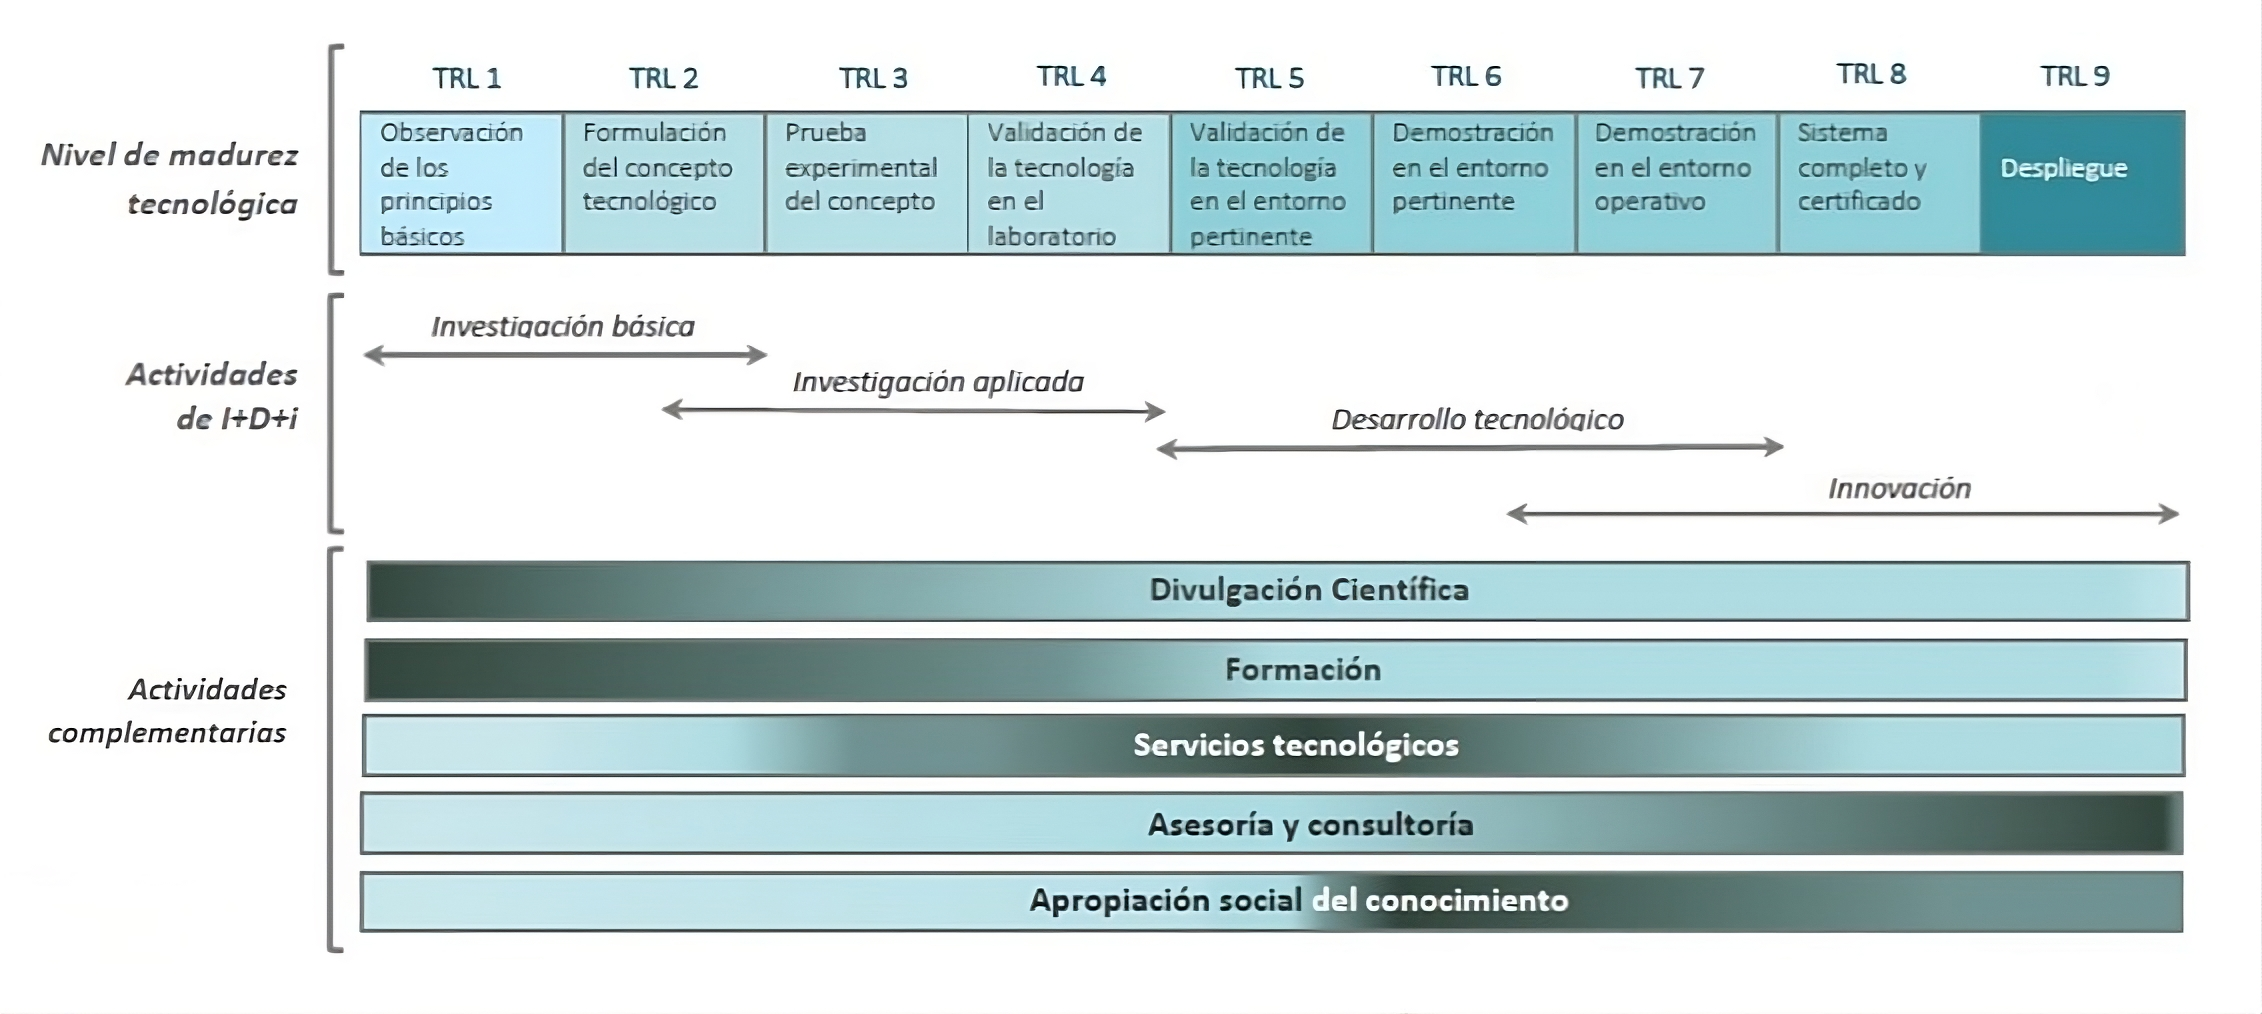
\includegraphics[width=\textwidth]{Figuras/trl.png}
    \caption{Niveles de TLR}
    \label{fig:trl}
\end{figure}

Este enfoque metadológico permitió aplicar los conocimientos adquiridos a lo largo de la formación profesional, con el fin de impulsar tanto el desarrollo como la validación de tecnologías en un contexto práctico y pertinente.
\\ \\
Teniendo en cuenta esta metodología de investigación, se siguió una secuencia de etapas orientadas a garantizar un proceso eficiente.  En primer lugar, se realizó una búsqueda bibliográfica para recopilar información relevante sobre el desarrollo de las habilidades seleccionadas, así como los métodos educativos y tecnologías de enseñanza disponibles. Posteriormente, se desarrolló la fase de diseño y construcción del software, utilizando diversas tecnologías web y herramientas de desarrollo. Una vez finalizada esta etapa, se procedió a la recolección de datos y evaluación mediante encuestas y actividades de desempeño, con el fín de analizar la efectividad del software en el desarrollo de habilidades blandas. Finalmente, se examinaron los datos obtenidos para elaborar conclusiones y formular recomendciones para ajustes o posibles mejoras futuras en la plataforma.
\section{Metodología de desarrollo de software}
La elección de una metodología de desarrollo de software adecuada resultó fundamental,
ya que simplificó el trabajo y proporcionó un marco claro y coherente para la ejecución del proyecto. Por esta razón, se compararon distintas metodologías ágiles, como se evidencia en la tabla \ref{tab:metodologias-agiles} con el objetivo de seleccionar aquella que mejor se ajustará a la naturaleza del trabajo de grado.
\\ 
\\
Dada la naturaleza del proyecto, se optó por analizar metodologías ágiles debido a su flexibilidad y eficiencia, aspectos cruciales para un desarrollo individual. Debido a la posibilidad de cambios en los requerimientos y objetivos del proyecto, una metodología ágil como Scrum, Kanban o Extreme Programming (XP) permitió manejar la incertidumbre de manera efectiva gracias a su enfoque simple, retroalimentación constante y adaptación al cambio. Es importante mencionar que, aunque estas metodologías fueron concebidas para equipos completos de desarrollo, muchos de sus conceptos pudieron aplicarse a un equipo conformado por un único desarrollador, tales como la planificación, la refactorización del código y el diseño simple del mismo.
\\
\\
Scrum no es una metodología de desarrollo de software, es un marco de gestión de proyectos de metodología ágil que los equipos utilizan para organizarse por cuenta propia y trabajar en aras de alcanzar un objetivo común. Caracterizado por un conjunto de ceremonias, herramientas y funciones que, de forma coordinada, ayudan a los equipos entregar proyectos de forma eficiente \cite{Amazon2024}.
\\
\\
Kanban es una metodología ágil que se basa en la visualización del flujo de trabajo y la carga de éste, su filosofía es centrada en la mejora continua, donde las tareas se extraen de una lista de acciones pendientes en un flujo de trabajo constante \cite{Martins2024}. Al utilizar tableros Kanban para representar visualmente las actividades organizadas por columnas (Las columnas más básicas son: trabajo pendiente, en progreso y terminado), el desarrollador puede identificar fácilmente cuellos de botella y ajustar la carga de trabajo según sea necesario. La ausencia de sprints permite una mayor flexibilidad en la planificación y ejecución de tareas, lo que puede ser beneficioso para proyectos donde los requisitos y objetivos pueden cambiar con frecuencia.
\\
\\
El Extreme Programming es una metodología ágil, formulada por Kent Beck, basada en la comunicación, la reutilización del código desarrollado y la retroalimentación. Su objetivo es promover la aplicación de apropiadas prácticas de ingeniería al momento de crear software. Por ejemplo, la programación en parejas y las revisiones de código promueven la colaboración y la detección temprana de errores. Las pruebas unitarias automatizadas y la integración continua garantizan la estabilidad y la funcionalidad del software en todo momento.  
\\
\\
\begin{table}[H]
    \centering
    \footnotesize
    \setlength{\tabcolsep}{3pt} 
    \renewcommand{\arraystretch}{1.2}
    \begin{tabular}{| m{2.5cm} | m{2.8cm} | m{2.8cm} | m{2.8cm} | m{2.8cm} |}
        \hline
        \textbf{Característica} & \textbf{Scrum} & \textbf{Kanban} & \textbf{Extreme Programming} & \textbf{Scrumban} \\
        \hline
        \textbf{Enfoque} & Iterativo con sprints fijos & Continuo & Iterativo e incremental & Híbrido entre Scrum y Kanban \\
        \hline
        \textbf{Roles definidos} & Product Owner, Scrum Master, Equipo & No hay roles predefinidos & cliente, programador, tester, tracker, entrenador, y consultor. & Puede incluir roles de Scrum o no \\
        \hline
        \textbf{Ceremonias} & Reuniones diarias, Sprint Planning, Sprint Review, Sprint Retrospective & No hay ceremonias predefinidas & Pair programming, integración continua, pruebas unitarias & Puede incluir ceremonias de Scrum o no \\
        \hline
        \textbf{Duración de iteraciones} & Sprints de duración fija (usualmente 1-4 semanas) & Continuo sin duración fija de iteraciones & Iteraciones cortas (1-3 semanas) & Iteraciones si se usan, no son fijas \\
        \hline
        \textbf{Tablero de trabajo} & Tablero Scrum (pendiente, en progreso, completado) & Tablero Kanban (Columnas personalizadas) & No tiene un tablero específico & Puede utilizar un tablero Kanban o Scrum \\
        \hline
        \textbf{Mejora continua} & Retrospectivas al final de cada sprint & Mejora continua sin restricciones de tiempo & Mejora continua, con énfasis en la calidad del código y feedback del cliente & Retrospectivas y mejora continua de Kanban \\
        \hline
        \textbf{Adaptabilidad} & Media (cambios tras cada sprint) & Alta (cambios en cualquier momento) & Altamente adaptable (ajustes en tiempo real) & Muy alta (combinación de Scrum y Kanban) \\
        \hline
        \textbf{Indicado para} & Proyectos con requisitos cambiantes y entrega incremental & Proyectos con demandas variadas y prioridades cambiantes & Proyectos donde la calidad y pruebas son críticas & Entornos que buscan estructura de Scrum con flexibilidad de Kanban \\
        \hline
        \textbf{Tamaño del equipo} & Idealmente de 3 a 9 personas & No hay restricciones específicas & No hay restricciones específicas & Puede variar dependiendo de la implementación \\
        \hline
    \end{tabular}
    \caption{Comparación de metodologías ágiles}
    \label{tab:metodologias-agiles}
\end{table}
Tras describir las tres mencionadas metodologías ágiles y considerando las particularidades del proyecto, Scrum fue descartado ya que resultó demasiado rígido para un proyecto individual, con sprints fijos y la necesidad de roles múltiples que no se alinearon bien con la naturaleza fluida de un proyecto gestionado por una sola persona. Tampoco se consideró Kanban debido a su falta de estructura periódica que garantizara la continuidad y el seguimiento del progreso en un proyecto individual. Por último, Extreme Programming (XP) no se contempló como una opción viable debido a la poca aplicabilidad de sus prácticas en un escenario individual de desarrollo.
\\
\\
Finalmente, emergió Scrumban como la opción más adecuada por diversas razones clave. En primer lugar, integró la flexibilidad de Kanban, lo cual fue ideal para adaptarse a la variabilidad en la carga de trabajo y a las prioridades cambiantes sin la necesidad de adherirse a los sprints fijos de Scrum. Además, ofreció un marco que ayudó a mantener el enfoque y la organización, facilitando la gestión del tiempo y del proyecto en solitario, asegurando que se mantuviera el progreso hacia los objetivos establecidos. Esto fue fundamental para un proyecto individual donde las necesidades evolucionaron rápidamente, como fue el caso del desarrollo de módulos educativos que requirieron revisiones frecuentes basadas en retroalimentación o nuevos hallazgos.
\section{Metodología de gestión de actividades}
Para la gestión de actividades del proyecto, se utilizó un tablero Kanban adaptado al enfoque Scrumban. Este tablero permitió visualizar el estado de cada tarea mediante columnas (“Pendientes”, “En progreso” y “Hecho”), lo que facilitó la organización, el seguimiento y la identificación de cuellos de botella durante todo el proceso.
\\ 
\\
Cada actividad del proyecto se representó como una tarjeta ubicada en la columna correspondiente según su estado. A medida que avanzaba el desarrollo, las tarjetas se movieron entre columnas, lo que proporcionó una visión clara y actualizada del progreso. Asimismo, el backlog se refinó continuamente, añadiendo nuevas tareas según surgieron requerimientos adicionales o ajustes necesarios en funcionalidades.
\\
\\
Este enfoque permitió una gestión ágil y adaptable, favoriciendo la priorización dinámica, la mejora continua y la rápida incorporación de cambios sin necesidad de ciclos cerrados o iteraciones fijas.

\begin{figure}[H]
\centering
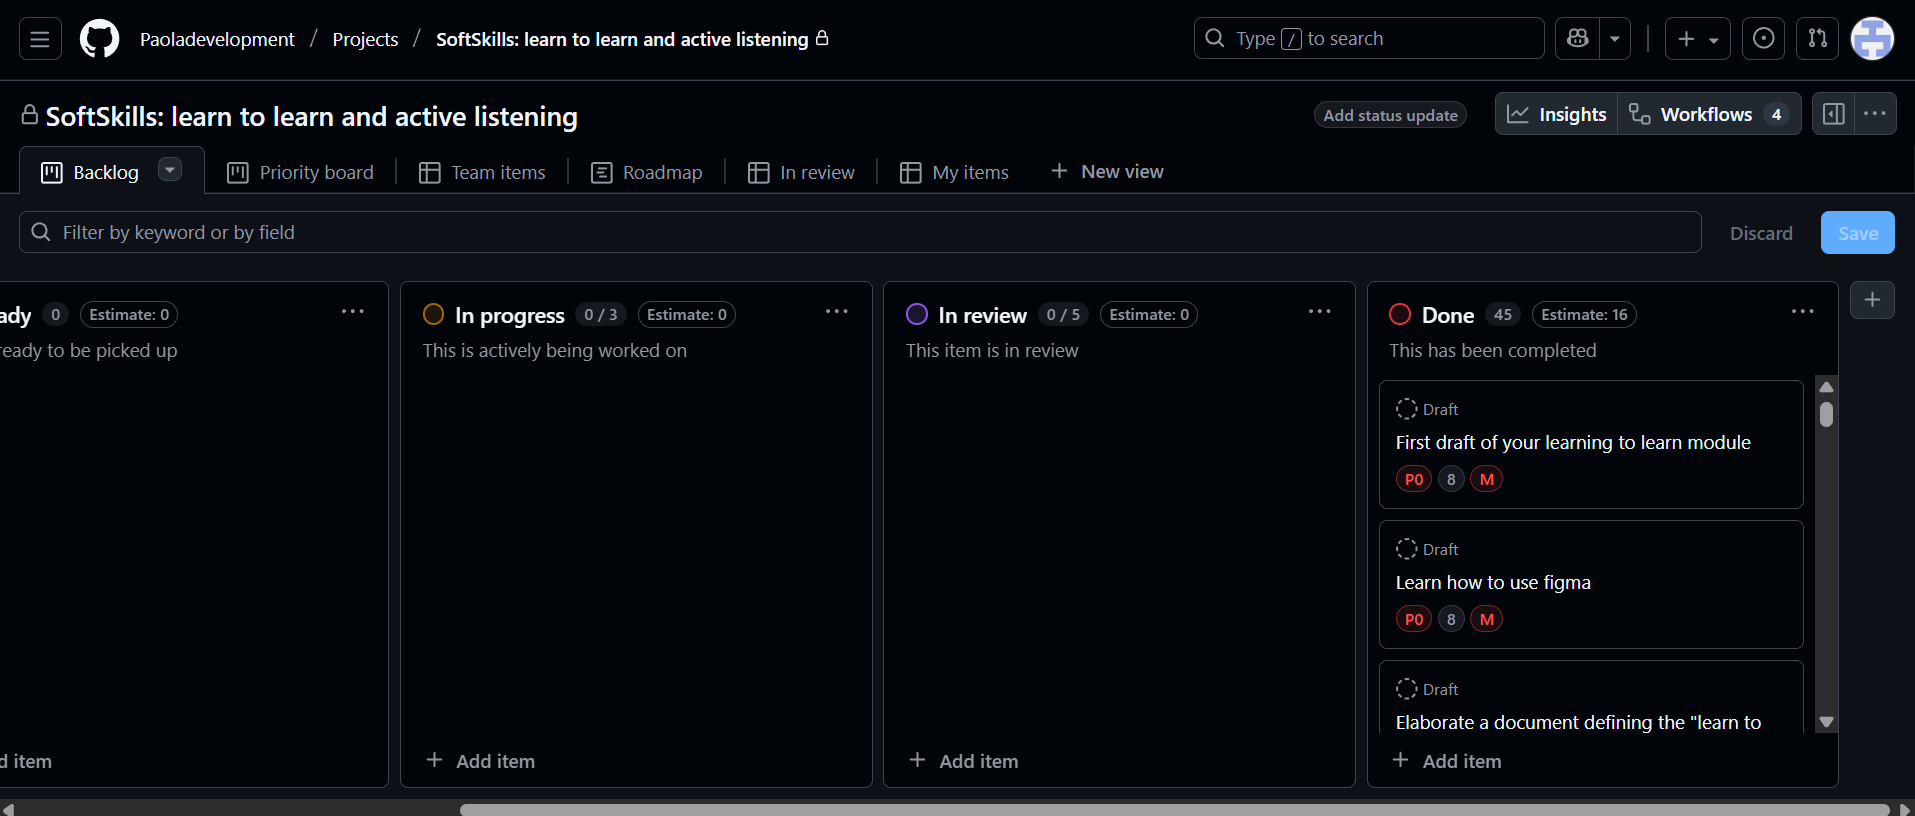
\includegraphics[width=\textwidth]{Figuras/tablero_github_projects.png}
\caption{Tablero Kanban del proyecto implementado en GitHub Projects.}
\label{fig:tablero_github}
\end{figure}

\subsection{Fase de definición y planificación inicial}

\begin{itemize}
    \item \textbf{Se definieron los objetivos del proyecto:}
    \begin{itemize}
        \item Se establecieron los objetivos generales y específicos.
        \item Se identificaron los entregables principales y los resultados esperados.
    \end{itemize}

    \item \textbf{Se creó el backlog inicial del proyecto:}
    \begin{itemize}
        \item Se listaron todas las tareas necesarias para desarrollar los módulos del sistema.
        \item Se priorizaron las tareas según su urgencia e impacto en el proyecto.
    \end{itemize}
\end{itemize}

\subsection{Fase de preparación y análisis de requisitos}

\begin{itemize}
    \item \textbf{Se recopilaron los requisitos del sistema:}
    \begin{itemize}
        \item Se realizaron sesiones de análisis para identificar y documentar los requisitos funcionales y no funcionales relacionados con los módulos de aprendizaje y escucha activa.
    \end{itemize}

    \item \textbf{Se analizaron, refinaron y validaron los requisitos:}
    \begin{itemize}
        \item Se detallaron, aclararon y reorganizaron los requisitos para asegurar su correcta comprensión y viabilidad técnica.
    \end{itemize}

    \item \textbf{Se actualizó el backlog:}
    \begin{itemize}
        \item Se añadieron nuevas tareas relacionadas con los requisitos identificados, incorporando refinamientos según su complejidad o dependencia.
    \end{itemize}
\end{itemize}

\subsection{Fase de diseño}

\begin{itemize}
    \item \textbf{Se diseñó la arquitectura del sistema:}
    \begin{itemize}
        \item Se elaboraron diagramas de la estructura general, se definieron los componentes principales del sistema y se establecieron las interacciones entre ellos.
    \end{itemize}

    \item \textbf{Se diseñó la interfaz de usuario:}
    \begin{itemize}
        \item Se desarrollaron prototipos de la interfaz del módulo Aprender a Aprender y del módulo de entrenamiento de escucha activa, definiendo elementos visuales y la experiencia de usuario (UX).
    \end{itemize}
\end{itemize}

\subsection{Fase de implementación}

\begin{itemize}
    \item \textbf{Se desarrollaron los módulos interactivos:}
    \begin{itemize}
        \item Se programaron las funcionalidades del sistema, incluyendo el módulo de gestión del aprendizaje, el editor de roadmaps y el módulo gamificado de escucha activa.
    \end{itemize}

    \item \textbf{Se integraron los componentes:}
    \begin{itemize}
        \item Se implementaron los diferentes elementos del backend y frontend, asegurando su correcto funcionamiento en conjunto y validando la comunicación entre los componentes.
    \end{itemize}

    \item \textbf{Se gestionó el trabajo con Scrumban:}
    \begin{itemize}
        \item El backlog se refinó continuamente y se utilizó el tablero Kanban para mover las tareas a través de las columnas “Pendiente”, “En Progreso” y “Hecho”, garantizando un flujo constante de avance.
    \end{itemize}
\end{itemize}

\subsection{Fase de pruebas}

\begin{itemize}
    \item \textbf{Se realizaron pruebas de usuario:}
    \begin{itemize}
        \item Se permitió que usuarios del sistema interactuaran con la plataforma, recopilando sus comentarios para identificar oportunidades de mejora que podrán incorporarse en futuras iteraciones.
    \end{itemize}
\end{itemize}

%%%%%%%%%%%%%%%%%%%%%%%%%%%%%%Capitulo 5%%%%%%%%%%%
\chapter{Revisión de literatura}
\markboth{Revisión de literatura}{Revisión de literatura}
Para el cumplimiento de los dos primeros objetivos específicos del trabajo, se llevó a cabo una revisión de literatura orientada, en primer lugar, a identificar las teorías y enfoques clave relacionadoscon el aprendizaje autónomo y continuo, así como las estrategias efectivas que fortalecen la capacidad de aprender a aprender. En segundo lugar, esta revisión tuvo como propósito investigar las metodologías y técnicas empleadas para fomentar la escucha activa durante las interacciones comunicativas, tomando como referencia la literatura académica y las mejores prácticas en el campo de la comunicación interpersonal.
\\
\\
El análisis bibliográfico consideró investigaciones recientes sobre metacognición, aprendizaje autorregulado, fijación de metas, estrategias de aprendizaje y procesos de autorreflexión, aspectos que permiten comprender de manera integral la competencia de aprender a aprender. Asimismo, se revisaron estudios centrados en la comprensión auditiva, la escucha activa, la atención, la interpretación de mensajes y las dinámicas de comunicación efectiva, los cuales aportan lineamientos para el fortalecimiento de esta habilidad mediante actividades estructuradas y deliberadas.
\\
\\
Adicionalmente, esta revisión permitió establecer la relación directa entre los aportes de literatura y las funcionalidades implementadas en la plataforma. Elementos como la estructura de metas--objetivos--tareas, las autoevaluaciones, el uso de estrategias de seguimiento del tiempo y la incorporación de desafíos auditivos con retroalimentación inmediata se sustentan en marcos teóricos ampliamente documentados.

\section{Metodología de la revisión}

Para esta revisión se empleó una metodología estructurada que incluyó:

\begin{itemize}
    \item \textbf{Búsqueda bibliográfica:} Se consultaron bases de datos académicas reconocidas, entre ellas IEEE Xplore, ACM Digital Library, ScienceDirect, Scopus y Google Scholar. Adicionalmente, se revisaron libros, capítulos y artículos de acceso abierto relacionados con metacognición, aprendizaje autorregulado, estrategias de aprendizaje y comunicación interpersonal.

    \item \textbf{Criterios de inclusión:} Se consideraron artículos publicados entre 2010 y 2024 que abordaran alguno de los siguientes temas: teorías y enfoques sobre aprendizaje autónomo y continuo, modelos y estrategias de aprendizaje autorregulado, fijación de metas, uso de ePortfolios, estrategias de gestión del tiempo, comprensión auditiva, escucha activa, interacción comunicativa y prácticas pedagógicas para el fortalecimiento de habilidades de comunicación. También se incluyeron estudios que presentaran resultados empíricos o propuestas metodológicas aplicables al contexto educativo universitario.

    \item \textbf{Palabras clave:} Para la búsqueda se emplearon combinaciones de términos en español e inglés, tales como: “aprendizaje autorregulado”, “metacognición”, “learn to learn”, “self-regulated learning”, “goal setting strategies”, “ePortfolio for learning”, “active listening”, “listening comprehension”, “communication skills”, “interpersonal communication” y “listening strategies”.

    \item \textbf{Revisión de artículos seleccionados:} Para el componente de aprendizaje autónomo, se analizaron los artículos recopilados en la tabla de estudios sobre \textit{Learn to Learn} (véase \hyperref[anexo:learn_to_learn]{Anexo A}), los cuales abordan temas como autorregulación, fijación de metas, reflexión, motivación, gestión del tiempo y uso de tecnologías para apoyar procesos metacognitivos. En cuanto al componente de escucha activa, se revisaron artículos que abordan el procesamiento cognitivo y metacognitivo de la comprensión auditiva, incluyendo la identificación de ideas clave, el parafraseo, la verificación de la interpretación, la segmentación del discurso, la memoria de trabajo, y el uso de recursos digitales, actividades guiadas y herramientas gamificadas para fortalecer la precisión interpretativa y la atención en tareas auditivas (véase \hyperref[anexo:escucha_activa]{Anexo B}).

    \item \textbf{Análisis comparativo:} Finalmente, se identificó cómo los hallazgos de la literatura se aplican en las funcionalidades implementadas en los módulos de la plataforma, con el propósito de asegurar que cada componente desarrollado se sustentara en enfoques y prácticas respaldadas por la investigación académica.
\end{itemize}

\section{Síntesis de estudios sobre \textit{Learn to Learn}}

La revisión de literatura realizada permitió identificar un conjunto de enfoques, teorías y estrategias que fundamentan el desarrollo del módulo \textit{Learn to Learn}. Los estudios seleccionados abordan componentes esenciales del aprendizaje autónomo y autorregulado, tales como la metacognición, la fijación de metas, la planificación, la gestión del tiempo, la motivación intrínseca y la reflexión continua. Estos elementos han sido ampliamente documentados en la literatura como factores determinantes para fortalecer la capacidad de los estudiantes de gestionar su propio proceso de aprendizaje.
\\
\\
A partir del análisis de los artículos incluidos (véase \hyperref[anexo:learn_to_learn]{Anexo A}), se elaboró una tabla sintetizada que reúne los aportes más significativos de cada estudio y su relación directa con las funcionalidades implementadas en el módulo. Aunque algunos trabajos presentan modelos o fundamentos teóricos, otros ofrecen hallazgos empíricos, propuestas metodológicas o marcos prácticos, razón por la cual la síntesis integra distintos tipos de contribuciones relevantes para el desarrollo del módulo.
\\
\\
Esta síntesis busca mostrar de manera clara cómo cada concepto o estrategia identificada en la literatura contribuye al diseño del modelo de metas--objetivos--tareas, a las prácticas de autorreflexión y a las herramientas de seguimiento utilizadas en la plataforma.
\\
\\
La Tabla~\ref{tab:syntesis_learn_to_learn} reúne los principales estudios analizados para fundamentar el módulo Learn to Learn, organizados según el concepto central abordado en cada artículo, la contribución específica del estudio y su aplicación en los componentes del módulo.

\begin{center}
\footnotesize
\setlength{\tabcolsep}{3pt}
\renewcommand{\arraystretch}{1.2}

    \begin{longtable}{| m{4.2cm} | m{3cm} | m{4.5cm} | m{4.5cm} |}
    \caption{Síntesis de estudios relevantes para el módulo \textit{Learn to Learn}}
    \label{tab:syntesis_learn_to_learn} \\
    \hline
    \textbf{Artículo} & \textbf{Concepto clave} & \textbf{Contribución del estudio} & \textbf{Aplicación en el módulo} \\
    \hline
    \endfirsthead

    \hline
    \textbf{Artículo} & \textbf{Concepto clave} & \textbf{Contribución del estudio} & \textbf{Aplicación en el módulo} \\
    \hline
    \endhead
    
    \hline \multicolumn{4}{c}{{\textit{Continúa en la siguiente página}}} \\
    \endfoot
    
    \hline
    \endlastfoot
    
    \textit{Hacia una nueva conceptualización del Aprender a Aprender} (Caena \& Stringher, 2020) \cite{caena_stringher_2020_aprender} &
    Conceptualización de AaA &
    El estudio redefine el Aprender a Aprender como una hiper-competencia que integra procesos metacognitivos, autorregulatorios y socio-afectivos para dirigir el aprendizaje de manera consciente. Propone un proceso ejecutivo que permite planificar, monitorear y evaluar el propio aprendizaje, impulsado por la autonomía como necesidad psicológica clave. Además, evidencia que el AaA implica ajustarse y responder a distintas tareas, entornos y demandas socioculturales, mostrando que no es una habilidad aislada sino un conjunto articulado de procesos que apoyan la autorregulación y la adaptación del aprendiz &
    Sustenta la definición del módulo como una competencia transversal que integra la fijación de metas, la reflexión y procesos de autorregulación del aprendizaje. \\
    \hline
    
    \textit{Learning how to learn and assessment for learning: a theoretical inquiry} (Black et al., 2007) \cite{black_etal_2007_learning} &
    AaA y evaluación formativa &
    Analiza cómo la evaluación formativa (AfL) contribuye al desarrollo del aprender a aprender al promover la reflexión, el feedback accionable y la toma de conciencia del propio progreso. El estudio muestra que la retroalimentación continua y co-construida fortalece la autonomía del aprendiz, fomenta la intencionalidad en la toma de decisiones y crea un entorno social que facilita la autorregulación y la mejora del desempeño. &
    Fundamenta la integración de autoevaluaciones y retroalimentación continua para promover la reflexión, la autorregulación y la toma de decisiones que guían el progreso del estudiante en el módulo. \\
    \hline
    
    \textit{Becoming a self-regulated learner: an overview} (Zimmerman, 2010) \cite{Zimmerman2002}&
    Aprendizaje autorregulado (SRL) &
    Presenta el modelo cíclico de autorregulación del aprendizaje compuesto por las fases de planificación, ejecución y autorreflexión. El artículo describe procesos como la fijación de metas, el monitoreo estratégico, el control motivacional y la autoevaluación, mostrando cómo estos permiten al estudiante gestionar activamente su aprendizaje. &
    Sustenta la organización del módulo en torno a las fases de planificación, ejecución y reflexión, y respalda el uso de metas, objetivos, tareas y monitoreo del progreso como componentes centrales de la autorregulación. \\
    \hline
    
    \textit{Do students learn what they teach when generating teaching materials for others?} (Ribosa \& Durán, 2022) \cite{ribosa_duran_2022_teach}&
    Aprender enseñando &
    Meta-análisis que demuestra que crear materiales didácticos para otros mejora el aprendizaje del contenido enseñado. Explica que este proceso activa mecanismos cognitivos generativos (como organizar, seleccionar y transformar la información) que promueven una comprensión más profunda y una mejor estructuración del conocimiento. También evidencia que los materiales visuales y audiovisuales potencian más el aprendizaje que los textuales. &
    Se relaciona directamente con el módulo, ya que la construcción de los planes de aprendizaje (roadmaps) (mediante la formulación de metas, objetivos y tareas) exige que el estudiante estructure, organice y represente visualmente su proceso de aprendizaje. Este acto de generar una explicación o material visual activa los mismos procesos cognitivos generativos descritos en el aprendizaje por enseñanza, favoreciendo una comprensión más profunda. \\
    \hline
    
    \textit{Personal OKRs: A tool for academic goal setting} (2023) \cite{lertladaluck_2023_personal_okrs}&
    Fijación de metas (OKRs) &
    El estudio implementa el marco OKR como herramienta para establecer metas académicas y demuestra, mediante una intervención de 16 semanas, que el uso de objetivos claros, resultados clave medibles y revisiones periódicas favorece la calidad del establecimiento de metas. Los hallazgos muestran una mejora significativa en el componente de metas basadas en datos (considerar experiencias previas, habilidades e información externa) impulsada por el seguimiento frecuente y la autorreflexión. &
    Alinea la estructura del módulo Learn to Learn (metas, objetivos, tareas y seguimiento) con los principios del marco OKR. Asimismo, fundamenta la incorporación de procesos de revisión continua, reflexión y ajuste del plan de aprendizaje \\
    \hline
    
    \textit{Implementing a Self-Regulated Oriented ePortfolio} (Alexiou \& Paraskeva, 2014) \cite{alexiou_paraskeva_2014_eportfolio}&
    ePortfolio y SRL &
    Presenta un ePortfolio orientado a la autorregulación construido sobre el modelo cíclico de Zimmerman, donde los estudiantes establecen metas, seleccionan estrategias, registran evidencias y reflexionan sobre su progreso. Los resultados muestran una mejora significativa en la calidad del establecimiento de metas tras su uso, indicando que el ePortfolio fortalece el monitoreo del aprendizaje, la identificación de fortalezas y dificultades, y la capacidad de diseñar estrategias de mejora. &
    Se relaciona con el módulo al fundamentar el uso de registros de progreso, reflexiones guiadas y seguimiento continuo del aprendizaje. Esta correspondencia se refleja particularmente en el formulario de reporte de aprendizaje que el estudiante completa al finalizar una meta, donde evalúa sus avances, dificultades y estrategias, alineándose con las prácticas de autorreflexión promovidas en los ePortfolios orientados a la autorregulación. \\
    \hline
    
    \textit{What Makes Adults Choose to Learn} (2018) \cite{broek_etal_2023_adults_choose}&
    Agencia y motivación &
    Analiza los factores que estimulan o inhiben la decisión de los adultos de aprender, destacando el papel de la motivación intrínseca, la relevancia personal, las emociones, la autoeficacia y el apoyo social. También identifica barreras como la falta de tiempo, experiencias negativas previas y la ausencia de claridad en los objetivos. El estudio subraya que la agencia del aprendiz (la sensación de control, autonomía y alineación con sus metas reales) es determinante para iniciar y sostener procesos de aprendizaje. &
    Justifica la personalización del módulo, ya que el estudio demuestra que la decisión de aprender depende de factores individuales como la motivación, la autonomía, la relevancia personal y las barreras percibidas. La formulación de metas propias, el reconocimiento de dificultades durante la reflexión final de cada meta y la adaptación del plan de aprendizaje (roadmap) responden directamente a las necesidades reales del adulto aprendiz. \\
    \hline
    
    \textit{Supporting students’ goal setting process using chatbot} (Du et al., 2021) \cite{du_etal_2021_chatbot_goals} &
    Apoyo digital a metas &
    El estudio implementa un chatbot basado en el marco SMART para guiar a los estudiantes en la fijación de metas al inicio de un curso en línea. A través de preguntas estructuradas y recomendaciones personalizadas, el chatbot ayudó a los estudiantes a clarificar y visualizar sus objetivos, formular metas más realistas y tomar conciencia del valor de establecer intenciones antes de comenzar a aprender. Los resultados evidencian que esta intervención digital fortalece la planificación inicial dentro del proceso de autorregulación del aprendizaje. &
    El estudio respalda el uso de apoyo digital para guiar la formulación de metas y pasos concretos, lo cual se refleja en el módulo mediante Aithena, el agente IA encargado de generar un plan de aprendizaje inicial a partir de los intereses, conocimientos previos y necesidades del estudiante. \\
    \hline
    
    \textit{Video Game Design for Learning to Learn} (Pasqualotto et al., 2023) \cite{pasqualotto_2023_videogame_learn2learn} &
    Diseño gamificado &
    El estudio analiza principios de diseño de videojuegos que favorecen el aprendizaje, destacando la importancia de la retroalimentación continua, la progresión por niveles, el ajuste dinámico de la dificultad y la estructuración guiada de la experiencia. Estos elementos mantienen la motivación, orientan la atención hacia los objetivos relevantes y permiten un avance gradual y significativo en las habilidades a desarrollar. &
    Respaldan la estructura progresiva del módulo, en la que el aprendizaje se organiza en pasos guiados (metas → objetivos → tareas), permitiendo que el estudiante avance de manera gradual y consciente, con apoyo estructurado durante la planificación y claridad sobre el progreso en cada etapa. \\
    \hline

    \end{longtable}
\end{center}

\section{Síntesis de estudios sobre Active Listening}
La revisión de literatura realizada para el módulo de \textit{Active Listening} permitió identificar un conjunto de enfoques, prácticas pedagógicas y procesos cognitivos que fundamentan el desarrollo de actividades orientadas al fortalecimiento de la comprensión auditiva. Los estudios seleccionados abordan componentes esenciales de la escucha activa, tales como la atención sostenida, la identificación de ideas clave, el parafraseo, la verificación de la comprensión, la segmentación del discurso, la memoria de trabajo y el monitoreo metacognitivo. Estos elementos han sido ampliamente documentados en la literatura como factores que influyen de manera directa en la precisión interpretativa y en la capacidad de reconstruir significados a partir de información auditiva limitada.
\\
\\
A partir del análisis de los artículos incluidos (véase \hyperref[anexo:active_listening]{Anexo B}), se elaboró una tabla que sintetiza los aportes más relevantes de cada estudio y su relación con las funcionalidades implementadas en el módulo. Mientras algunos trabajos proponen estrategias instruccionales (como actividades guiadas de parafraseo, síntesis o práctica deliberada) otros ofrecen hallazgos empíricos sobre el impacto del procesamiento cognitivo y metacognitivo en la escucha, o bien exploran el papel de tecnologías interactivas, recursos multimedia y herramientas gamificadas para mejorar la motivación, la atención y la claridad interpretativa durante tareas auditivas.
\\
\\
Esta síntesis busca evidenciar cómo cada concepto, estrategia o enfoque identificado en la literatura contribuye al diseño de las rondas auditivas del módulo, a los mecanismos de retroalimentación inmediata y a las dinámicas interactivas que favorecen la precisión interpretativa y el monitoreo de la comprensión durante las tareas auditivas.
\\
\\
La Tabla~\ref{tab:syntesis_active_listening} presenta los estudios analizados, organizados según su concepto central, la contribución específica del artículo y su aplicación en los componentes del módulo de escucha activa.

\begin{center}
\footnotesize
\setlength{\tabcolsep}{3pt}
\renewcommand{\arraystretch}{1.2}

\begin{longtable}{| m{4.2cm} | m{3cm} | m{4.5cm} | m{4.5cm} |}
\caption{Síntesis de estudios relevantes para el módulo \textit{Active Listening}}
\label{tab:syntesis_active_listening} \\
\hline
\textbf{Artículo} & \textbf{Concepto clave} & \textbf{Contribución del estudio} & \textbf{Aplicación en el módulo} \\
\hline
\endfirsthead

\hline
\textbf{Artículo} & \textbf{Concepto clave} & \textbf{Contribución del estudio} & \textbf{Aplicación en el módulo} \\
\hline
\endhead

\hline \multicolumn{4}{c}{{\textit{Continúa en la siguiente página}}} \\
\endfoot

\hline
\endlastfoot

\textit{Active Listening for Engineering Students} (Novick, Realyvasquez and Ramirez, 2021) \cite{novick_2021_active_listening}  &
Entrenamiento estructurado en escucha activa &
El estudio identifica la escucha activa como una de las habilidades más demandadas por empleadores de ingenieros y desarrolla un conjunto de módulos formativos distribuidos a lo largo de un programa universitario. El artículo define la escucha activa en cuatro fases (pre-listening, during, post-listening inmediata y a largo plazo) e integra comportamientos concretos como evitar respuestas juiciosas, ofrecer retroalimentación verbal y no verbal adecuada, mantener la atención y formular preguntas para fomentar la expresión del interlocutor. Además, describe actividades pedagógicas efectivas (como roles de escucha, ejercicios de práctica deliberada, prompts guiados y reflexión posterior) que permiten a los estudiantes comprender, practicar y evaluar habilidades de escucha activa. &
Sustenta la inclusión de actividades auditivas estructuradas, dado que el estudio evidencia que la práctica guiada, el modelamiento y la retroalimentación inmediata fortalecen comportamientos esenciales de escucha activa. \\ \hline

\textit{Active Listening in Written Online Communication} (Bauer and Figl, 2008)  \cite{bauer_figl_2008_active_listening_online} &
Escucha activa en entornos sin señales no verbales &
El estudio analiza la aplicabilidad de las técnicas de escucha activa en comunicación escrita mediante mensajería instantánea, un contexto que carece de claves no verbales y presenta mayor riesgo de distracciones. Los resultados muestran que todas las técnicas clásicas de escucha activa (parafrasear, clarificar, preguntar, resumir y animar al interlocutor) aparecieron de manera consistente en las interacciones analizadas, demostrando que pueden usarse eficazmente incluso en entornos textuales. Sin embargo, el estudio identifica desafíos importantes: mensajes superpuestos que inducen malentendidos, distracciones frecuentes, dificultad para mantener la atención y limitaciones para expresar o interpretar emociones sin apoyo vocal o gestual. También se reconoce como ventaja la permanencia del texto, que permite revisar mensajes y apoyar la comprensión. &
El estudio respalda el diseño de actividades donde el estudiante debe comprender un mensaje exclusivamente a partir del contenido verbal, sin apoyo visual ni claves no verbales, tal como ocurre en las rondas de audio del módulo. Además, el artículo evidencia que la falta de atención sostenida y los malentendidos son problemas frecuentes en contextos sin claves no verbales, lo que respalda el uso de rondas secuenciales, repeticiones controladas del audio y retroalimentación inmediata en el módulo, ya que estos elementos ayudan a reforzar la comprensión y reducir errores interpretativos. \\ \hline

\textit{“Can You Repeat That?” Teaching Active Listening in Management Education} (Spataro and Bloch, 2018) \cite{spataro_bloch_2018_active_listening_management} &
Pedagogías de parafraseo, síntesis y práctica guiada &
El estudio propone un método pedagógico para enseñar escucha activa basado en autoevaluación, materiales instruccionales, práctica deliberada y reflexión estructurada. Demuestra que actividades guiadas que incluyen parafraseo, formulación de preguntas, síntesis y verificación de comprensión permiten a los estudiantes interiorizar las habilidades de escucha activa. Los resultados cuantitativos y cualitativos evidencian mejoras en la capacidad de describir estrategias de escucha, reconocer cuándo aplicarlas y transferirlas a nuevos contextos. &
Sustenta el uso de actividades que requieren parafrasear, sintetizar, completar información, identificar ideas centrales y formular preguntas de aclaración, tal como ocurre en los modos de juego Paraphrase, Summarize, Focus, Cloze y Clarify del módulo. El énfasis del estudio en la práctica deliberada y en ejercicios guiados respalda la estructura por rondas, la repetición controlada del audio y la retroalimentación inmediata, que permiten al estudiante internalizar gradualmente las habilidades de escucha activa. \\ \hline

\textit{The Relative Effectiveness of Active Listening in Initial Interactions} (Weger, Castle and Emmett, 2014) \cite{weger_castle_emmett_2014_relative_effectiveness} &
Efectos del parafraseo y retroalimentación empática &
El estudio compara el parafraseo con otros estilos de respuesta en interacciones iniciales y demuestra que las respuestas basadas en escucha activa incrementan significativamente la percepción de empatía y apoyo. Sin embargo, también evidencia que el parafraseo no garantiza que el hablante se sienta completamente comprendido, mostrando que la interpretación del mensaje puede diferir de la intención original. Estos hallazgos resaltan la complejidad de lograr una comprensión precisa incluso cuando se aplican técnicas de escucha activa. &
Refuerza el valor de actividades donde el estudiante compara su interpretación del mensaje con el contenido real, como ocurre en los modos de juego Paraphrase, Summarize, Focus y Clarify. El hallazgo de que el parafraseo no siempre conduce a una comprensión completa justifica el uso de retroalimentación inmediata en el módulo, permitiendo que el estudiante verifique si lo que entendió coincide con el mensaje original y ajuste progresivamente su precisión interpretativa a lo largo de las rondas. \\ \hline

\textit{Listening Strategy Applications by Learners under the Context of Multimodality} (Kao, Liao and Lan, 2017) \cite{kao_liao_lan_2017_listening_strategies} &
Estrategias de escucha y uso de estrategias metacognitivas bajo modalidades multimodales &
El estudio aporta evidencia empírica sobre cómo los estudiantes gestionan su proceso de comprensión auditiva mediante estrategias metacognitivas (tales como atención selectiva, atención dirigida, identificación de problemas y monitoreo) incluso cuando cambian las condiciones de apoyo (entorno multimodal 3D o ayudas impresas). La contribución central radica en demostrar que la regulación metacognitiva es un componente dominante y estable del proceso de escucha, más influyente que las variaciones en el tipo de apoyo visual disponible. &
Sustenta actividades del módulo que requieren regulación atencional, monitoreo de la comprensión y selección de información relevante. Modos como Focus, Summarize, Paraphrase y Cloze demandan atención dirigida, identificación de ideas clave y verificación de la interpretación, procesos alineados con las estrategias metacognitivas identificadas como predominantes en el estudio. \\ \hline

\textit{Promoting Listening Skills with an Educational Tool: VoScreen} (Merzifonluoğlu, 2023) \cite{merzifonluoglu_2023_voscreen} &
Gamificación aplicada a la comprensión auditiva &
El estudio demuestra que VoScreen, una herramienta basada en microvideos con retroalimentación inmediata, produce mejoras estadísticamente significativas en la comprensión auditiva de los estudiantes. El análisis cualitativo destaca beneficios adicionales como mayor motivación, exposición a acentos variados y la percepción de que el formato breve y repetitivo facilita una práctica sostenida. &
Sustenta el enfoque gamificado del módulo al validar el uso de desafíos auditivos cortos, retroalimentación inmediata y tareas breves que aumentan la motivación, la atención y la continuidad en la práctica de escucha. \\ \hline

\textit{Enhancing 21st Century Students’ Listening Skills via Augmented Reality and Mobile Applications} (Ismayatim et al., 2019) \cite{ismayatim_etal_2019_ar_listening} &
Tecnologías móviles y realidad aumentada aplicadas a prácticas de escucha &
El estudio analiza las percepciones de estudiantes universitarios sobre MyEVO, un módulo de escucha que integra realidad aumentada, dispositivos móviles y videos auténticos. Los resultados muestran una valoración ampliamente positiva: los estudiantes consideran que la combinación de audio y video facilita la comprensión del contenido, incrementa el interés y permite un aprendizaje más flexible e independiente. Asimismo, destacan que las prácticas basadas en AR son interactivas, modernas y fáciles de usar, y que la posibilidad de controlar el ritmo (pausar, repetir, revisar) favorece la experiencia de aprendizaje. &
Apoya el diseño del módulo al mostrar que entornos digitales interactivos que combinan estímulos auditivos con una interfaz multimedia incrementan el interés, la percepción de comprensión y la autonomía del estudiante, según las valoraciones reportadas. En nuestro caso, estos hallazgos respaldan el uso de audios breves integrados en una interfaz gamificada que permite controlar el ritmo de la actividad, repetir el contenido y participar en prácticas de escucha más dinámicas y accesibles. \\ \hline

\textit{La escucha activa y la memorización en la formación de intérpretes} (Bertozzi Díaz, 2021) \cite{bertozzi_2021_escucha_activa_interpretes} &
Memoria de trabajo, análisis del discurso y reconstrucción del mensaje &
El estudio presenta una experiencia didáctica centrada en la escucha activa y las técnicas de memorización para intérpretes en formación. Expone que la escucha activa implica operaciones cognitivas profundas como analizar la estructura del discurso, identificar ideas principales, distinguir información esencial de la redundante y mantener la atención sostenida. Asimismo, muestra que la memorización eficaz se basa en la segmentación del mensaje (chunking), la visualización mental, la identificación de palabras clave y la reconstrucción del contenido a partir de unidades significativas. Los resultados preliminares indican mejoras percibidas en reformulación, priorización y retención de discursos estructurados y no estructurados. &
Sustenta actividades del módulo que exigen retener información auditiva breve, reconstruir el mensaje, identificar patrones y sintetizar ideas. Apoya especialmente modos como Summarize, Paraphrase y Cloze, que requieren análisis del contenido, comprensión profunda y uso activo de la memoria de trabajo para reorganizar e interpretar fragmentos auditivos limitados. \\ \hline

\end{longtable}
\end{center}



%%%%%%%%%%%%%%%%%%%%%%%%%%%%%%Capitulo 6%%%%%%%%%%%
\chapter{Diseño de actividades y recursos educativos del prototipo}
\markboth{Diseño de actividades y recursos educativos del prototipo}{Diseño de actividades y recursos educativos del prototipo}
Este capítulo, correspondiente al objetivo específico 3, presenta el diseño de actividades gamificadas y de las experiencias interactivas que conforman el prototipo orientado a fortalecer las habilidades de aprender a aprender y escucha activa en estudiantes de ingeniería. El contenido se centra en la aplicación práctica de la fundamentación expuesta en la Revisión de Literatura, utilizando dichos lineamientos para definir la estructura de las actividades, seleccionar los recursos educativos apropiados y articular las acciones e interacciones que permiten que cada módulo favorezca el desarrollo de la habilidad que aborda.

\section{Actividades implementadas en el prototipo}

Esta sección describe las actividades implementadas en cada uno de los módulos del prototipo. Su propósito es presentar, de manera clara y estructurada, las acciones que realiza el estudiante dentro de la plataforma y la forma en que cada módulo articula sus funcionalidades para favorecer el desarrollo de las habilidades de aprender a aprender y escucha activa. La descripción de las actividades permite contextualizar el uso de los recursos educativos presentados en la sección siguiente.

\subsection{Actividades implementadas en el módulo aprender a aprender}

El módulo de aprender a aprender organiza sus actividades en torno a la planificación, ejecución y reflexión del proceso de aprendizaje del estudiante. Las actividades implementadas son:

\begin{itemize}

\item \textbf{Creación de roadmaps personalizados:} El estudiante puede generar un plan de aprendizaje mediante dos opciones: (1) una propuesta automática creada por el sistema a partir de sus intereses, conocimientos previos, estilo de aprendizaje y disponibilidad de tiempo, o (2) la construcción manual de un roadmap desde cero mediante el editor visual.

\item \textbf{Edición mediante un editor visual de planes de aprendizaje:} El prototipo incluye un editor gráfico donde el estudiante puede crear, modificar y reorganizar la estructura de su plan de aprendizaje. Este editor permite añadir objetivos, tareas, modificar descripciones, visualizar la relación entre componentes y estructurar el plan de manera clara e intuitiva.

\item \textbf{Conversión entre roadmap y plan accionable:} El sistema permite transformar un roadmap visual en una estructura detallada basada en metas, objetivos y tareas, así como convertir un plan accionable nuevamente en un roadmap editable. Esta función facilita alternar entre una vista general del aprendizaje y una versión operativa del plan, donde cada componente se vuelve ejecutable y rastreable, permitiendo que las tareas avancen por distintos estados (No iniciado, En progreso, En pausa, Completado).

\item \textbf{Exploración de planes de aprendizaje públicos:} El módulo ofrece un espacio para descubrir planes de aprendizaje creados por otros usuarios. El estudiante puede explorar, filtrar por autor o número de pasos, visualizar descripciones y revisar la estructura completa del plan antes de decidir si desea incorporarlo a su propio proceso.

\item \textbf{Copia y reutilización de planes públicos:} A partir de un plan de aprendizaje público, el estudiante puede crear una copia en su cuenta para adaptarlo a sus metas personales. Esta funcionalidad facilita el acceso a modelos de referencia y acelera la planificación inicial.

\item \textbf{Gestión de objetivos y tareas:} Una vez creado el roadmap o copiado un plan existente, el estudiante puede añadir, editar y organizar objetivos y tareas asociadas a sus metas de aprendizaje, estructurando el proceso en pasos concretos y alcanzables.

\item \textbf{Seguimiento del progreso mediante Kanban:} Las tareas asignadas a cada objetivo pueden gestionarse visualmente mediante un tablero Kanban con las columnas “Por hacer”, “En progreso”, “En pausa” y “Completado”, permitiendo al estudiante monitorear su avance y tomar decisiones informadas sobre su proceso.

\item \textbf{Desarrollo de tareas de aprendizaje:} Al seleccionar una tarea, el estudiante accede a su descripción completa y a los recursos asociados que apoyan su realización. El avance de la tarea (como iniciarla, pausarla o completarla) se gestiona mediante el movimiento de la tarjeta correspondiente dentro del tablero Kanban del objetivo.

\item \textbf{Agregación de recursos a las tareas:} Cada tarea admite la incorporación de recursos externos en distintos formatos (videos, artículos, documentos, libros o enlaces web). Esta funcionalidad permite que el estudiante disponga de materiales de apoyo directamente vinculados con la actividad que debe realizar.

\item \textbf{Registro de notas personales por tarea:} El módulo permite añadir notas asociadas a una tarea específica, facilitando que el estudiante registre ideas, recordatorios, reflexiones rápidas o información complementaria relevante para el desarrollo del aprendizaje.

\item \textbf{Autoevaluación y reflexión guiada al finalizar una tarea:} Al completar una tarea, el sistema presenta un conjunto de preguntas orientadas a la reflexión autorregulada. Estas incluyen la intención de aprendizaje, las estrategias utilizadas, las dificultades encontradas, los aspectos logrados y el plan de mejora para futuras actividades; además, el estudiante puede indicar si logró establecer una conexión con conocimientos previos.

\item \textbf{Acceso a reportes de aprendizaje:} El estudiante puede consultar un historial de autoevaluaciones asociadas a todas las tareas completadas. Este apartado permite ordenar y filtrar los reportes según fecha, nivel de dificultad o estado de ánimo, facilitando el análisis de patrones de desempeño y el fortalecimiento del monitoreo metacognitivo.

\item \textbf{Configuración de visibilidad de los planes de aprendizaje:} Cada roadmap puede configurarse como privado o público. En la modalidad pública, el plan puede compartirse mediante un enlace, lo que permite al estudiante controlar quién puede visualizar, copiar o reutilizar sus planes de aprendizaje dentro de la plataforma.

\end{itemize}

\begin{figure}[H]
    \centering
    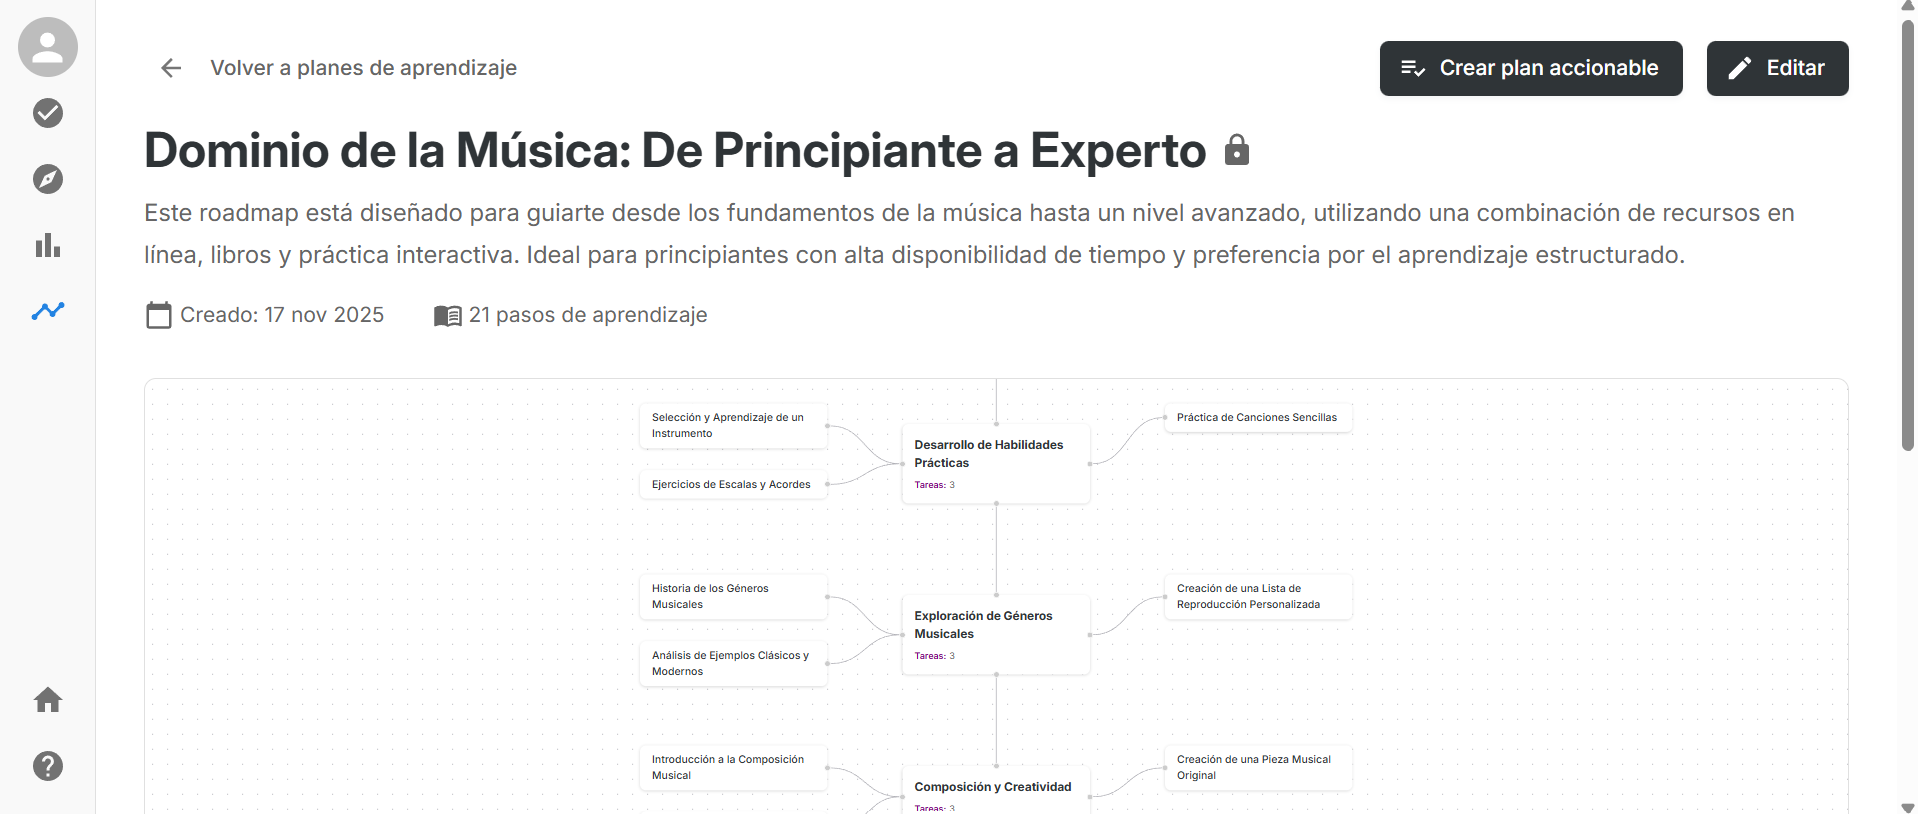
\includegraphics[width=\textwidth]{Figuras/interfaces_AaA/imagen_representativa_modulo_AaA.png}
    \caption{Vista representativa del módulo \textit{Aprender a Aprender}}
    \label{fig:modulo_aprender_a_aprender}
\end{figure}

\noindent Las interfaces que ilustran el funcionamiento de estas actividades se encuentran detalladas en el \hyperref[anexo:interfaces_aprender]{Anexo C}, organizadas en el mismo orden en que se presentan las actividades descritas.


\subsection{Actividades implementadas en el módulo de escucha activa} El módulo de escucha activa está estructurado como un conjunto de rondas de juego, en las que el estudiante interactúa con audios generados automáticamente y ejercicios diseñados para fortalecer habilidades específicas de comprensión auditiva. Las actividades implementadas son:

\begin{itemize}

\item \textbf{Configuración inicial de la sesión de juego:} Antes de comenzar una sesión, el estudiante puede definir parámetros como el número total de rondas, el máximo de repeticiones permitidas por ronda, los tipos de prompts habilitados (descriptivo, evento histórico, instructivo, diálogo, diálogo narrado) y el nivel de dificultad. También puede decidir si desea reutilizar desafíos existentes o generar nuevos contenidos de forma dinámica.

\item \textbf{Inicio de la sesión de juego:} Tras configurar la sesión, el estudiante inicia una experiencia compuesta por una secuencia de rondas. Cada ronda se prepara con un tipo de prompt y un modo de juego específico, de acuerdo con la configuración seleccionada.

\item \textbf{Reproducción del audio:} En cada ronda, el estudiante escucha un clip de audio generado mediante IA, cuyo contenido varía según el tipo de prompt seleccionado. El sistema asegura que cada audio esté alineado con el estilo, dificultad y duración establecidos.

\item \textbf{Resolución del ejercicio según el modo de juego:} Una vez escuchado el audio, el estudiante completa el ejercicio correspondiente al modo de juego asignado: selección múltiple (Focus), completar espacios (Cloze), paráfrasis (Paraphrase), resumen (Summarize) o formulación de preguntas de aclaración (Clarify).

\item \textbf{Manejo de repeticiones de audio por ronda:} Cada ronda permite un número limitado de reproducciones del audio, configurado al iniciar la sesión. El estudiante puede volver a escuchar el clip para reforzar su comprensión antes de responder el ejercicio, siempre dentro del máximo permitido. Las repeticiones aplican únicamente a la escucha del audio, no al envío de la respuesta.

\item \textbf{Envío de respuesta y retroalimentación:} Tras enviar la respuesta, el sistema genera retroalimentación inmediata que incluye la puntuación obtenida, los aciertos, los errores y, en el caso de Clarify, la comparación entre las preguntas formuladas por el estudiante y las preguntas de referencia generadas por el sistema.

\item \textbf{Progresión automática a la siguiente ronda:} Una vez revisada la retroalimentación, el sistema dirige al estudiante a la siguiente ronda. Este proceso continúa hasta completar el total de rondas configuradas.

\item \textbf{Finalización de la sesión:} Al completar todas las rondas, el sistema presenta un resumen global del desempeño de la sesión: número de rondas, puntuación total, respuestas correctas e incorrectas, así como un histórico detallado de cada ronda.

\item \textbf{Revisión detallada de cada ronda:} El estudiante puede acceder a un reporte individual de cada ronda, que incluye el audio utilizado, la respuesta enviada, la puntuación asignada, los intentos realizados y (cuando aplica) la comparación entre sus preguntas y las preguntas de referencia del sistema.

\end{itemize}

\begin{figure}[H]
    \centering
    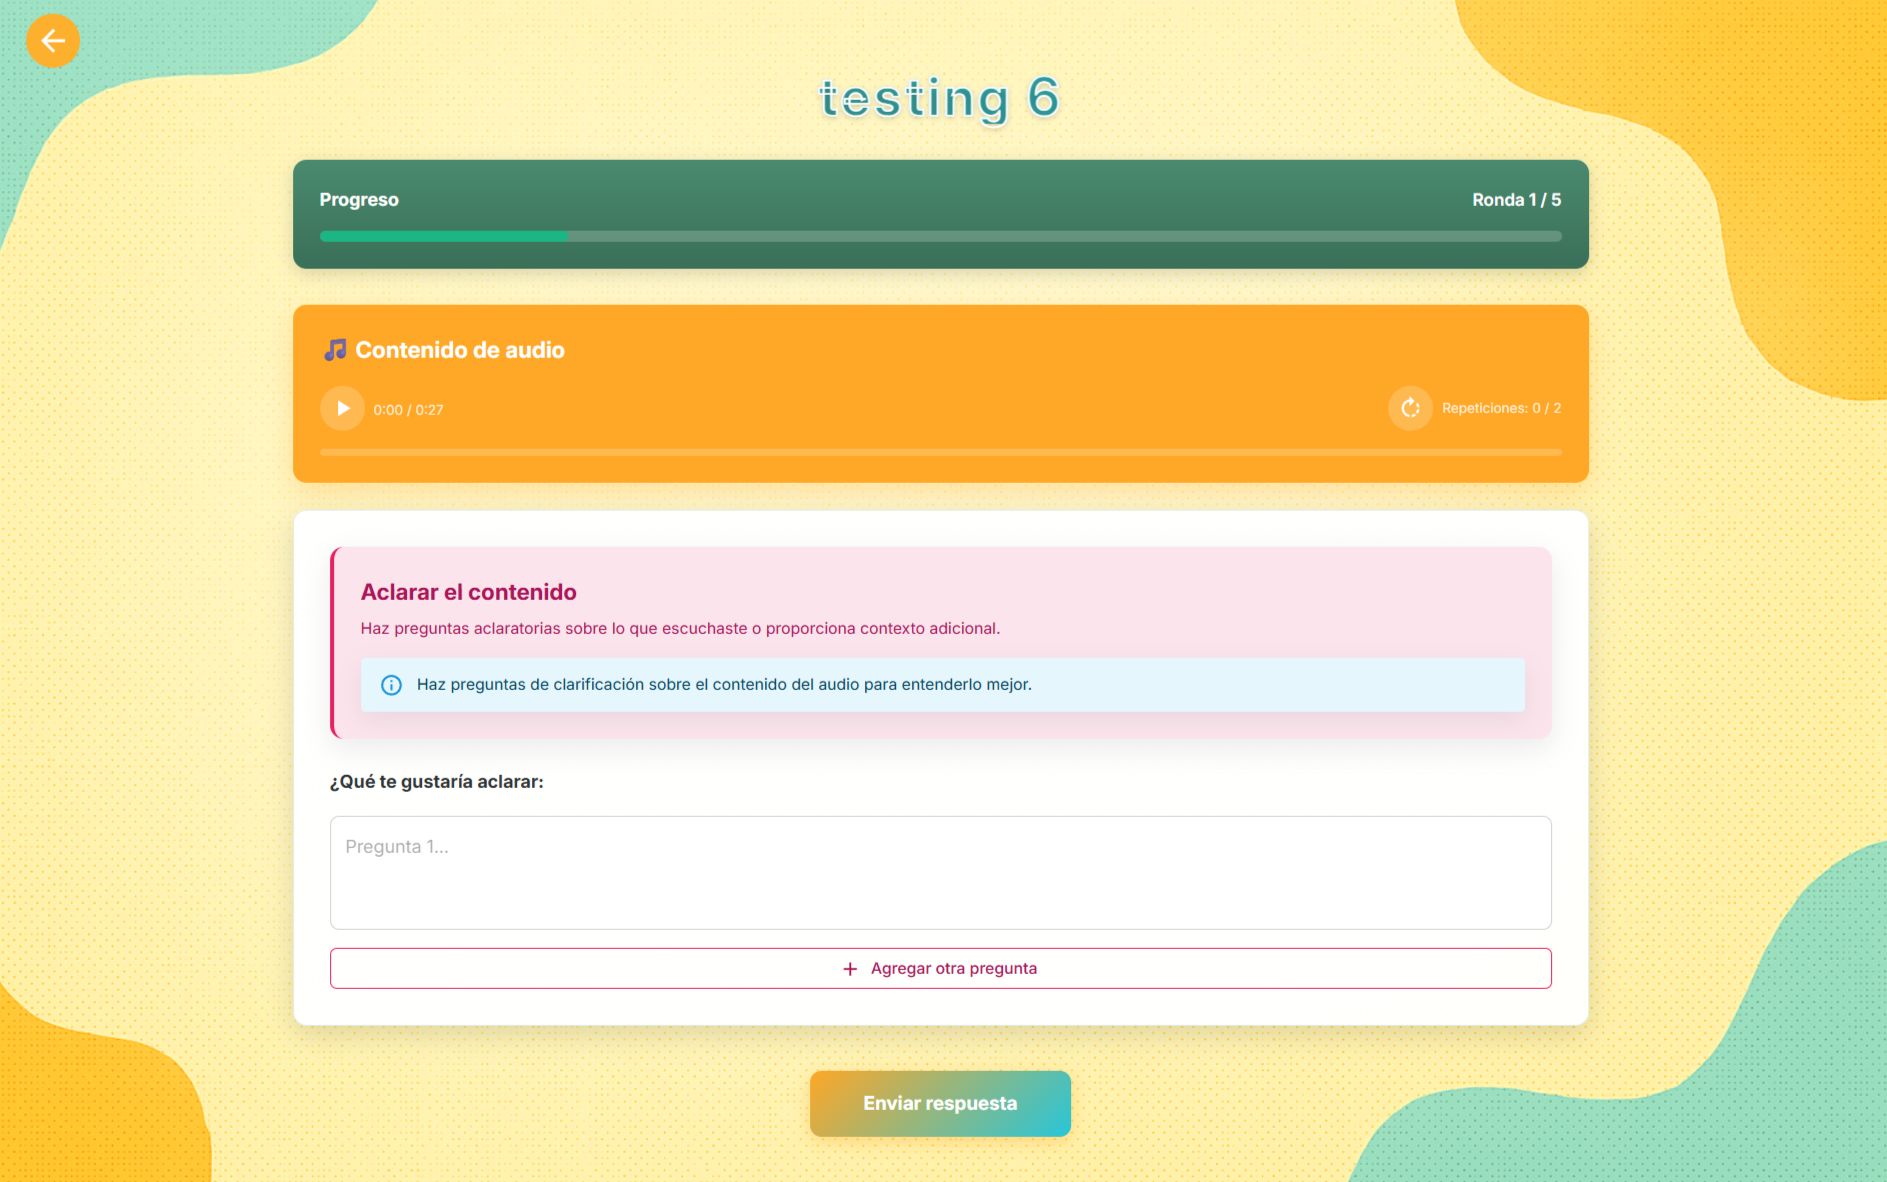
\includegraphics[width=\textwidth]{Figuras/interfaces_EA/ea_ronda_juego.png}
    \caption{Vista representativa del módulo \textit{Escucha activa}}
    \label{fig:modulo_escucha_activa}
\end{figure}

\noindent Las interfaces que ilustran el funcionamiento de estas actividades se encuentran detalladas en el \hyperref[anexo:interfaces_escucha_activa]{Anexo D}, organizadas en el mismo orden en que se presentan las actividades descritas.

\section{Recursos educativos empleados}
Esta sección presenta los recursos educativos empleados en cada uno de los módulos del prototipo. En el contexto de este proyecto, se entiende por recursos educativos a los contenidos, herramientas, apoyos y elementos instruccionales que facilitan el aprendizaje del estudiante y que contribuyen al desarrollo de las habilidades de aprender a aprender y escucha activa.

\subsection{Recursos educativos empleados en el módulo aprender a aprender}
Los recursos educativos integrados en este módulo apoyan al estudiante en la planificación, organización y monitoreo de su propio proceso de aprendizaje:

\begin{itemize}

\item \textbf{Estructura metas–objetivos–tareas:} Organización del proceso de aprendizaje en metas, objetivos y tareas que facilitan la planificación, la priorización y la organización del trabajo personal, fortaleciendo habilidades de autorregulación.

\item \textbf{Roadmaps generados por IA o construidos manualmente:} Planes estructurados de aprendizaje creados a partir de la información ingresada por el estudiante (intereses, conocimientos previos, estilo de aprendizaje y disponibilidad de tiempo), que orientan la planificación inicial y permiten visualizar la secuencia de objetivos y tareas.

\item \textbf{Tablero Kanban:} Herramienta visual que permite al estudiante gestionar el estado de sus tareas a través de columnas como “Por hacer”, “En progreso”, "En pausa", “Completado”, fomentando el monitoreo continuo y la toma de decisiones informada.

\item \textbf{Autoevaluaciones y reflexiones guiadas:} Preguntas y espacios de reflexión que permiten analizar avances, identificar dificultades, evaluar estrategias empleadas y establecer acciones de mejora, fortaleciendo la autorreflexión y el aprendizaje autónomo.

\end{itemize}

\noindent Las interfaces asociadas a estas actividades se encuentran detalladas en el \hyperref[anexo:interfaces_escucha_activa]{Anexo D}, donde se ilustran los distintos momentos de interacción del estudiante durante la sesión de juego, desde su configuración inicial hasta la revisión del desempeño por ronda.



\subsection{Recursos educativos empleados en el módulo de escucha activa}
Los recursos educativos incorporados en este módulo estructuran las actividades de escucha y orientan la interacción del estudiante con los diferentes tipos de ejercicios. A través de estos recursos, el módulo facilita un entrenamiento progresivo de las habilidades vinculadas a la escucha activa.

\begin{itemize}

\item \textbf{Audios generados con IA:} Clips de audio producidos mediante modelos de lenguaje y síntesis de voz, cuyo contenido varía según el tipo de prompt seleccionado (descriptivo, instructivo, diálogo, diálogo narrado, entre otros). Esta variación temática permite ofrecer ejercicios de comprensión auditiva en contextos diversos y más cercanos a situaciones reales.

\item \textbf{Guiones pedagógicos por modo de juego:} Textos adaptados a cada modo de juego (Selección múltiple (Focus), Completar espacios [Cloze], Paráfrasis [Paraphrase], Resumir [Summarize] y Aclarar [Clarify]) que guían al estudiante en habilidades clave de comprensión auditiva, como identificar información relevante, completar contenido, parafrasear, resumir o aclarar ideas.


\item \textbf{Retroalimentación inmediata:} Comentarios automáticos generados al finalizar cada ronda de juego, que permiten al estudiante identificar aciertos, errores y aspectos a mejorar, guiando el proceso de comprensión y fomentando la práctica continua.

\end{itemize}

\section{Elementos de gamificación integrados en el prototipo}
El diseño del prototipo incorpora elementos de gamificación con el fin de aumentar el compromiso, la motivación y la participación del estudiante en las actividades de aprendizaje, tal como lo sugiere la literatura sobre gamificación en entornos digitales. De acuerdo con Watini y Setyowati (2023) \cite{watini2023gamification}, la gamificación consiste en integrar dinámicas, mecánicas y elementos de juego en contextos no lúdicos para promover conductas deseadas, estimular la participación y fortalecer la experiencia del usuario en plataformas de e-learning.
\\
\\
La aplicación de estos principios permite compensar algunas limitaciones propias del aprendizaje en línea, como la falta de interacción emocional presente en entornos presenciales. Desde modelos como el Fogg Behavior Model, la gamificación actúa sobre tres dimensiones clave: motivación, habilidad y disparadores (triggers), favoreciendo estados de alta concentración y participación sostenida durante las actividades educativas.
\\
\\
En coherencia con estos lineamientos, el prototipo integra diversos elementos de gamificación cuidadosamente seleccionados para los módulos de aprender a aprender y escucha activa, con el propósito de fomentar la constancia, facilitar el avance progresivo y aumentar la satisfacción del estudiante durante el uso de la plataforma.

\subsubsection{Elementos de gamificación implementados}

A partir de las recomendaciones presentadas por Watini y Setyowati en su estudio sobre gamificación en entornos de e-learning \cite{watini2023gamification}, se seleccionaron e integraron diversos elementos que refuerzan la motivación, el compromiso y la continuidad en el aprendizaje. La siguiente subsección describe cómo cada uno de estos elementos se materializó en el prototipo desarrollado.

\paragraph{a. Progresión y estructura por niveles}

El prototipo organiza las actividades en etapas claramente definidas (rondas, tareas, objetivos), siguiendo la recomendación de dividir los contenidos en unidades pequeñas que permitan avances graduales y logros frecuentes. Este principio de progresión incremental, señalado por Watini y Setyowati \cite{watini2023gamification}, incrementa la percepción de avance y fortalece la motivación intrínseca.
\\
\\
En el módulo de escucha activa, cada ronda funciona como un “nivel” que se desbloquea al completar la ronda anterior.  
En el módulo aprender a aprender, la estructura metas–objetivos–tareas opera como una jerarquía gamificada de progresión.

\paragraph{b. Recompensas y retroalimentación inmediata}

La retroalimentación instantánea constituye uno de los mecanismos más efectivos para aumentar la motivación en e-learning, al proporcionar claridad sobre el desempeño y reforzar conductas deseadas \cite{watini2023gamification}. El prototipo incorpora este elemento mediante:

\begin{itemize}
    \item Puntuación inmediata al finalizar cada ronda del módulo de escucha activa, diferenciando aciertos, errores y aspectos por mejorar.
    \item Retroalimentación continua en el módulo aprender a aprender mediante autoevaluaciones y la actualización del estado de las tareas en el tablero Kanban.
\end{itemize}

\paragraph{c. Indicadores visuales de progreso}

Según el estudio, los indicadores de progreso (como barras de avance o estados visibles) son efectivos para mantener la motivación al permitir al estudiante monitorear su trayectoria y visualizar cuánto ha completado \cite{watini2023gamification}. En el prototipo se implementaron:

\begin{itemize}
    \item Barra de progreso asociada a cada ronda del módulo de escucha activa.
    \item Estados del Kanban: \textit{Por hacer}, \textit{En progreso}, \textit{En pausa}, \textit{Completado}.
    \item Resúmenes de desempeño al finalizar las sesiones de escucha activa.
\end{itemize}

\paragraph{d. Desafíos y dificultad ajustada}

El artículo enfatiza que los retos deben estar equilibrados para mantener el interés sin generar frustración \cite{watini2023gamification}. Atendiendo a esta recomendación, el prototipo incorpora ajustes dinámicos de dificultad:

\begin{itemize}
    \item En escucha activa, el estudiante puede configurar el nivel de dificultad, lo que ajusta parámetros como la duración del audio, la complejidad semántica y las exigencias del modo de juego.
    \item En aprender a aprender, la dificultad se ve reflejada en la complejidad de las tareas y del proceso de planificación.
\end{itemize}

\paragraph{e. Personalización y sentido de agencia}

Permitir al usuario tomar decisiones dentro del sistema aumenta el sentido de control y, por tanto, la motivación intrínseca \cite{watini2023gamification}. En el prototipo se adoptó este principio mediante:

\begin{itemize}
    \item Configuración personalizada de sesiones: dificultad, tipos de prompt, número de rondas, reutilización de desafíos.
    \item Creación, edición y adaptación de planes de aprendizaje propios.
    \item Copia y personalización de planes públicos para ajustarlos a metas individuales.
\end{itemize}

\paragraph{f. Anticipación y preparación del siguiente paso}

Watini y Setyowati resaltan que la anticipación de la siguiente actividad reduce el abandono y mantiene al usuario dentro del flujo de aprendizaje \cite{watini2023gamification}. El prototipo incorpora este principio mediante:

\begin{itemize}
    \item Transición automática entre rondas en escucha activa.
    \item Indicaciones claras sobre la siguiente tarea, objetivo o ronda a completar.
    \item Resúmenes finales que orientan sobre el desempeño y los pasos siguientes.
\end{itemize}

\paragraph{g. Socialización indirecta como motivador}

Aunque sin competencia directa, el prototipo integra un componente de socialización indirecta, coherente con los principios de comunidad y reconocimiento mencionados por el artículo \cite{watini2023gamification}. Este elemento se expresa mediante:

\begin{itemize}
    \item Exploración de planes de aprendizaje públicos creados por otros estudiantes.
    \item Acceso a estructuras y estrategias ajenas que sirven como inspiración y validación social.
\end{itemize}

Como consolidación de los elementos de gamificación descritos y su relación con los módulos desarrollados, en el \hyperref[anexo:gamificacion]{Anexo E} se presenta una tabla comparativa que resume su implementación en el prototipo.

%%%%%%%%%%%%%%%%%%%%%%%%%%%%%%Capitulo 7%%%%%%%%%%%
\chapter{Implementación del prototipo}
\markboth{Implementación del prototipo}{Implementación del prototipo}
\section{Arquitectura general del sistema}
El prototipo se desarrolló bajo una arquitectura cliente-servidor, siguiendo el modelo descrito en los principios fundamentales de aplicaciones web: el cliente ejecuta la interfaz gráfica e inicia las solicitudes HTTP, mientras que el servidor procesa la lógica de negocio, administra los datos y coordina los servicios necesarios para responder cada petición.
\\
\\
Bajo este enfoque, el prototipo integra un cliente web construido con React y un servidor implementado con FastAPI, complementados por bases de datos relacionales y no relacionales, servicios externos de inteligencia artificial y un sistema de almacenamiento de audio para los desafíos del módulo de Escucha Activa. Cada componente cumple un rol específico dentro del flujo cliente-servidor, lo que permite mantener una arquitectura escalable, modular y fácilmente extensible.

\section{Tecnologías seleccionadas}
A partir de la arquitectura cliente-servidor descrita anteriormente, se seleccionó un conjunto de tecnologías que resultan apropiadas para satisfacer los requerimientos funcionales y no funcionales del prototipo. La selección consideró criterios como compatibilidad, mantenibilidad, facilidad de integración con servicios externos, disponibilidad de documentación y capacidad para soportar flujos que requieren una interacción continua entre el usuario y el sistema (como la manipulación de un editor visual) e inteligencia artificial.

\subsection{Tecnologías para el desarrollo del frontend}

\begin{table}[H]
\centering
\footnotesize
\begin{tabular}{| m{3.5cm} | m{11cm} |}
\hline
\textbf{Tecnología} & \textbf{Descripción y uso en el prototipo} \\
\hline
React & Biblioteca para la construcción de interfaces web dinámicas basada en componentes reutilizables. Permitó desarrollar el módulo de \textit{Aprender a Aprender}, el editor de roadmaps y las pantallas interactivas del módulo de \textit{Escucha Activa}. \\
\hline
TypeScript & Añade tipado estático al ecosistema de React, mejorando la robustez del código, evitando errores comunes y facilitando el mantenimiento. \\
\hline
Material-UI (MUI) & Framework de componentes estilizados que permite construir interfaces consistentes, accesibles y responsivas, reduciendo el esfuerzo necesario en diseño visual y maquetación. \\
\hline
React Flow & Librería especializada en la construcción de editores visuales basados en grafos. Fue utilizada para implementar el editor de roadmaps, permitiendo arrastrar, conectar, organizar y almacenar nodos y relaciones. \\
\hline
Zustand & Biblioteca ligera para la gestión de estado global. Se utilizó en la administración de sesiones de juego, manejo del roadmap, estados del editor y sistema global de notificaciones (toasts). \\
\hline
React Query & Herramienta para la sincronización eficiente entre el frontend y la API, que gestiona el cacheo, revalidación y actualización de datos provenientes del backend. \\
\hline
\end{tabular}
\caption{Tecnologías utilizadas en el desarrollo del frontend del prototipo.}
\end{table}

\subsection{Tecnologías para el desarrollo del backend}

\begin{table}[H]
\centering
\footnotesize
\begin{tabular}{| m{3.5cm} | m{11cm} |}
\hline
\textbf{Tecnología} & \textbf{Descripción y uso en el prototipo} \\
\hline
FastAPI & Framework para la creación de APIs en Python, caracterizado por su rendimiento, soporte para tipado estático y documentación automática. Fue utilizado para gestionar la lógica de negocio, los endpoints REST y la integración con los modelos de IA y los servicios de generación de audio. \\
\hline
SQLModel & ORM que fue utilizado para definir las entidades del dominio y facilitar su interacción con PostgreSQL, combinando características de Pydantic y SQLAlchemy. \\
\hline
Pydantic & Fue utilizado para la validación de datos en los esquemas de entrada y salida, garantizando integridad y coherencia entre cliente y servidor. \\
\hline
Uvicorn & Servidor ASGI que se empleó para la ejecución eficiente de la API en entornos de desarrollo y despliegue. \\
\hline
\end{tabular}
\caption{Tecnologías empleadas en el desarrollo del backend del prototipo.}
\end{table}

\subsection{Tecnologías para la gestión de bases de datos}

\begin{table}[H]
\centering
\footnotesize
\begin{tabular}{| m{3.5cm} | m{11cm} |}
\hline
\textbf{Base de datos} & \textbf{Descripción y uso en el prototipo} \\
\hline
PostgreSQL & Base de datos relacional que fue utilizada para almacenar información estructurada, incluyendo usuarios, metas, objetivos, tareas, sesiones de juego, rondas, desafíos auditivos y evaluaciones. Proporcionó integridad, transaccionalidad y consultas eficientes durante la ejecución del prototipo. \\
\hline
MongoDB & Base de datos NoSQL orientada a documentos, que fue empleada para el almacenamiento flexible de los roadmaps de aprendizaje, sus nodos, tareas asociadas y el layout visual generado por el editor de React Flow. \\
\hline
\end{tabular}
\caption{Tecnologías utilizadas para la gestión de datos en el prototipo.}
\end{table}

\subsection{Tecnologías para el uso de modelos de inteligencia artificial}

\begin{table}[H]
\centering
\footnotesize
\begin{tabular}{| m{3.5cm} | m{11cm} |}
\hline
\textbf{Tecnología} & \textbf{Descripción y uso en el prototipo} \\
\hline
OpenAI API & Servicio que fue utilizado para la generación de contenido textual, incluyendo desafíos auditivos, instrucciones, mensajes guía y retroalimentación semántica para los modos de juego. \\
\hline
LangChain & Librería que fue empleada para estructurar prompts, gestionar herramientas, manejar cadenas y definir agentes conversacionales encargados de generar contenido educativo y metadatos para los desafíos del módulo de Escucha Activa. \\
\hline
LangGraph & Framework utilizado para la creación de agentes basados en grafos que permiten estructurar secuencias de razonamiento. Fue empleado para implementar el agente tutor responsable de generar roadmaps personalizados. \\
\hline
\end{tabular}
\caption{Tecnologías utilizadas para la integración con modelos de inteligencia artificial.}
\end{table}

\subsection{Tecnologías para la generación y almacenamiento de audio}

\begin{table}[H]
\centering
\footnotesize
\begin{tabular}{| m{3.5cm} | m{11cm} |}
\hline
\textbf{Tecnología} & \textbf{Descripción y uso en el prototipo} \\
\hline
ElevenLabs & Plataforma de síntesis de voz (TTS) que fue utilizada para generar audios de alta calidad a partir de los textos creados por los modelos de lenguaje. Permitió personalizar la voz, el estilo y el ritmo del audio en función de cada desafío. \\
\hline
Supabase Storage & Servicio de almacenamiento que fue utilizado para guardar los audios generados y obtener URLs públicas o firmadas para su reproducción en el frontend durante las sesiones de juego. \\
\hline
\end{tabular}
\caption{Tecnologías empleadas para la generación y almacenamiento de archivos de audio.}
\end{table}

\subsection{Tecnologías de despliegue}

\begin{table}[H]
\centering
\footnotesize
\begin{tabular}{| m{3.5cm} | m{11cm} |}
\hline
\textbf{Tecnología} & \textbf{Descripción y uso en el prototipo} \\
\hline
Vercel & Plataforma que fue utilizada para desplegar el frontend y el backend principal del prototipo, aprovechando funciones serverless, bajos tiempos de respuesta y despliegues automáticos vinculados al repositorio. \\
\hline
Railway & Plataforma de despliegue en la nube que fue utilizada para alojar el backend independiente del agente de generación de roadmaps. Su modelo de ejecución persistente resultó más adecuado que el enfoque serverless de Vercel para manejar los tiempos de procesamiento prolongados y la continuidad requerida por los agentes basados en LangChain y LangGraph. \\
\hline
\end{tabular}
\caption{Tecnologías utilizadas para el despliegue del prototipo.}
\end{table}


\section{Desarrollo del backend}
\subsection{Configuración del entorno}

Para la implementación del backend se configuró un entorno orientado a garantizar estabilidad, reproducibilidad y compatibilidad con los distintos servicios necesarios para el funcionamiento del prototipo. Este entorno se construyó sobre Python 3.11 y empleó un sistema de gestión de dependencias que permitió mantener versiones consistentes de librerías, asegurar un aislamiento apropiado y facilitar el despliegue en múltiples entornos de ejecución.
\\
\\
En esta etapa se configuraron los elementos fundamentales del backend, entre ellos:

\begin{itemize}
    \item \textbf{FastAPI como framework principal:} seleccionado por su rendimiento, asincronía nativa y capacidad para estructurar APIs de manera modular, manteniendo un alto nivel de claridad y escalabilidad en los controladores expuestos al frontend.

    \item \textbf{Gestión de dependencias mediante Poetry:} utilizada para administrar el entorno virtual del proyecto, asegurar versiones específicas de paquetes y garantizar reproducibilidad durante las fases de desarrollo, pruebas y despliegue.

    \item \textbf{Manejo de asincronía en el framework:} aunque FastAPI ofrece soporte nativo para ejecución asincrónica, la implementación actual utiliza principalmente operaciones síncronas tanto en el acceso a la base de datos como en los servicios auxiliares.

    \item \textbf{CORS como mecanismo de interoperabilidad:} configurado para permitir la comunicación segura entre el cliente web y el backend, controlando los orígenes autorizados durante la interacción entre módulos.
\end{itemize}

\subsection{Arquitectura y organización}
 Para la implementación del backend se empleó una arquitectura monolítica modular organizada por capas, un enfoque adecuado para prototipos que requieren simplicidad operativa y una separación clara de responsabilidades. Bajo este esquema, el sistema se estructura en capas diferenciadas (exposición de API, lógica de negocio, acceso a datos e integración con servicios externos) que trabajan de manera coordinada dentro de una misma aplicación.

\subsubsection{Capa de exposición o API}
Corresponde al punto de entrada de todas las solicitudes provenientes del frontend. En esta capa se gestionan aspectos como:

\begin{itemize}
    \item Recepción de peticiones HTTP.
    \item Validación de los datos de entrada.
    \item verificación de autenticación mediante tokens JWT.
    \item Estandarización de los datos de respuesta.
\end{itemize}

La API actúa únicamente como un intermediario: procesa las solicitudes de forma superficial y delega la lógica principal a la capa de servicios, donde se ejecutan las reglas y operaciones del sistema. Este enfoque permite mantener controladores livianos, fáciles de mantener y coherentes con buenas prácticas de desarrollo.

\subsubsection{Capa de servicios o lógica de negocio}
En esta capa se concentra el núcleo del comportamiento del sistema. Aquí se implementan las reglas específicas de cada módulo, así como operaciones complejas que requieren coordinar múltiples entidades y fuentes de datos. Entre sus responsabilidades se incluyen:

\begin{itemize}
    \item Validación de reglas de negocio.
    \item Gestión de transacciones.
    \item Coordinación entre bases de datos relacionales y documentos NoSQL.
    \item Actualizaciones en cascada (por ejemplo, el estado de un objetivo según el progreso de sus tareas).
    \item Orquestación de procesos que combinan datos, IA y almacenamiento externo.
\end{itemize}

La lógica del módulo \textit{Aprender a Aprender} se construyó sobre servicios responsables de manejar metas, objetivos y tareas, mientras que el módulo \textit{Escucha Activa} incorpora servicios especializados para administrar sesiones de juego, rondas, desafíos, evaluación y generación de audio.

\subsubsection{Capa de acceso a datos}
Esta capa define el mecanismo mediante el cual los servicios interactúan con las bases de datos. El prototipo combina:

\begin{itemize}
    \item \textbf{PostgreSQL}, utilizado para almacenar información estructurada como usuarios, metas, objetivos, tareas, sesiones de juego, rondas y desafíos.
    \item \textbf{MongoDB}, empleado para representar estructuras jerárquicas completas (por ejemplo, un learning goal con todos sus objetivos y tareas) y para gestionar los roadmaps generados mediante IA.
\end{itemize}

Mientras PostgreSQL garantiza integridad referencial y transacciones ACID, MongoDB ofrece flexibilidad y acceso eficiente a documentos completos. La sincronización entre ambas fuentes de datos permite aprovechar las fortalezas de cada una sin duplicar lógica innecesariamente.

\subsubsection{Capa de integración con servicios externos}
Algunas funcionalidades centrales del prototipo dependen de servicios especializados, entre ellos:

\begin{itemize}
    \item \textbf{Modelos de lenguaje (OpenAI + LangChain):} utilizados para generar desafíos auditivos, construir prompts dinámicos, evaluar las respuestas proporcionadas por los participantes y procesar salidas estructuradas mediante esquemas validados.

    \item \textbf{Síntesis de voz (ElevenLabs):} responsable de convertir el contenido textual de los desafíos en audio, empleando voces configurables y modelos multilingües.

    \item \textbf{Almacenamiento en la nube (Supabase Storage):} utilizado para guardar de manera persistente los archivos de audio generados y exponerlos mediante URLs públicas accesibles desde el cliente.
\end{itemize}

Esta capa permite encapsular las interacciones con servicios externos y abstraer su complejidad del resto del sistema.

\subsection{Visión general de componentes}

El backend se encuentra organizado en un conjunto de componentes que estructuran las
funcionalidades del sistema y facilitan la separación de responsabilidades. Estos componentes
están organizados en los directorios principales del proyecto y actúan como bloques funcionales que
permiten gestionar modelos de datos, lógica de negocio, validaciones, acceso a bases de datos y
servicios externos.
\\
\\
Tanto la estructura de carpetas como la descripción de cada componente se presentan en la
Figura~\ref{fig:estructura_backend_textual} y en la Tabla~\ref{tab:componentes_backend},
respectivamente.

\begin{figure}[H]
\centering
\begin{verbatim}
backend/
|-- alembic/                 (Migraciones para la base de datos PostgreSQL)
|-- data/                    (Recursos estáticos y archivos auxiliares)
|-- enums/                   (Enumeraciones del sistema: estados, tipos y constantes)
|-- llm/                     (Integración con modelos de lenguaje y generación de contenidos)
|-- model/                   (Modelos SQLModel para PostgreSQL)
|-- mongo_service/           (Servicios para operaciones con MongoDB)
|-- nosql_models/            (Modelos de documentos NoSQL)
|-- nosql_schema/            (Esquemas de validación para documentos en MongoDB)
|-- router/                  (Endpoints de la API organizados por dominio funcional)
|-- schema/                  (Esquemas Pydantic para validación y respuesta)
|-- service/                 (Lógica de negocio y orquestación de procesos)
+-- utils/                   (Funciones auxiliares y utilidades compartidas)
\end{verbatim}
\caption{Estructura jerárquica de directorios del backend. Elaboración propia.}
\label{fig:estructura_backend_textual}
\end{figure}


\begin{table}[H]
\centering
\footnotesize
\setlength{\tabcolsep}{8pt}
\renewcommand{\arraystretch}{1.25}
\begin{tabular}{|p{3cm}|p{11cm}|}
\hline
\textbf{Componente} & \textbf{Descripción} \\
\hline

\textbf{alembic} &
Gestiona las migraciones del esquema de PostgreSQL. Incluye configuraciones, plantillas y
versiones que permiten crear o modificar tablas, columnas y restricciones de forma controlada. \\
\hline

\textbf{data} &
Contiene scripts de inicialización y carga de datos de prueba (\textit{seed}), utilizados durante el
desarrollo para poblar PostgreSQL y MongoDB con usuarios, metas, objetivos y otros elementos
del prototipo. \\
\hline

\textbf{enums} &
Contiene las enumeraciones que representan valores fijos del backend, incluyendo modos de juego, estados de sesión, roles de usuario, tipos de recurso y otros valores tipados utilizados a lo largo del sistema. \\
\hline

\textbf{llm} &
Implementa la integración con modelos de lenguaje mediante LangChain y OpenAI. Incluye
clientes de LLM, generadores de desafíos auditivos, evaluadores de respuestas y cargadores de
prompts utilizados en el módulo de Escucha Activa. \\
\hline

\textbf{model} &
Define los modelos de datos persistentes basados en SQLModel, que representan tablas y
relaciones en PostgreSQL. Contiene entidades como usuarios, metas, objetivos, tareas, sesiones
de juego, rondas y desafíos. \\
\hline

\textbf{mongo\_service} &
Incluye servicios especializados para operar sobre MongoDB, gestionando documentos
jerárquicos asociados a metas, objetivos, tareas y roadmaps. Facilita la sincronización dual entre
PostgreSQL y la base documental. \\
\hline

\textbf{nosql\_models} &
Modelos Pydantic que representan la estructura de documentos almacenados en MongoDB,
particularmente para los roadmaps y sus componentes anidados. \\
\hline

\textbf{nosql\_schema} &
Esquemas para validar, serializar y convertir documentos NoSQL en modelos tipados. Proveen
el formato de entrada y salida en operaciones relacionadas con roadmaps. \\
\hline

\textbf{router} &
Expone los endpoints REST del backend. Cada archivo corresponde a un dominio funcional como
autenticación, metas, objetivos, tareas, roadmaps, desafíos o sesiones de juego. Los routers se encargan de recibir las solicitudes, aplicar las validaciones de entrada necesarias,
gestionar la autenticación y delegar la ejecución al nivel de servicios.
\\
\hline

\textbf{schema} &
Define los esquemas Pydantic utilizados para validar datos de entrada y estructurar las
respuestas de la API. Incluye schemas de creación, actualización, paginación y respuestas
especializadas para cada módulo. \\
\hline

\textbf{service} &
Implementa la lógica de negocio del sistema. Coordina operaciones entre modelos, gestiona reglas
de negocio, orquesta transacciones en PostgreSQL y sincroniza datos con MongoDB, además de
interactuar con servicios externos como OpenAI, ElevenLabs y Supabase Storage. \\
\hline

\textbf{utils} &
Contiene utilidades compartidas: configuración del sistema, clientes de PostgreSQL y MongoDB,
integraciones con almacenamiento y síntesis de voz, serializadores, validadores y funciones de
apoyo utilizadas en múltiples módulos. \\
\hline

\end{tabular}
\caption{Visión general de los componentes del backend}
\label{tab:componentes_backend}
\end{table}

\subsection{Diagramas de arquitectura}

Con el fin de complementar la descripción de la arquitectura presentada previamente, se incluyen diagramas detallados para cada uno de los componentes principales del sistema. Estos diagramas ilustran el flujo de interacción entre el cliente web, el servidor backend y las bases de datos empleadas, destacando las operaciones de lectura (\textbf{R}) y escritura (\textbf{W}) involucradas en cada funcionalidad.
\\

Cada descripción hace referencia a su respectivo diagrama arquitectónico, disponible en el \textbf{Anexo F}. Para mantener claridad y evitar redundancia, se mencionan únicamente las operaciones generales asociadas a cada componente, mientras que la definición completa de los endpoints puede consultarse en el \hyperref[anexo:endpoints]{\textbf{Anexo H}}.

\subsubsection{Gestión de metas de aprendizaje}

El componente encargado de la gestión de metas maneja operaciones de creación, consulta, actualización y eliminación de metas definidas por el usuario. Estas operaciones se realizan mediante solicitudes recibidas en la API y delegadas a los servicios correspondientes, los cuales coordinan la persistencia en PostgreSQL (\textbf{R/W}) y la sincronización con MongoDB para mantener la estructura jerárquica completa.
\\

El flujo detallado de esta interacción se presenta en el \hyperref[fig:anexoF-learning-goals]{\textbf{Anexo F.1}}.

\subsubsection{Gestión de objetivos}

El componente de objetivos permite administrar los elementos intermedios que estructuran cada meta. Incluye operaciones para crear objetivos, actualizar su estado, reorganizarlos y consultarlos de manera individual o agrupada. Estas operaciones se reflejan en PostgreSQL (\textbf{R/W}) y se sincronizan en MongoDB para garantizar una representación completa y eficiente en las interfaces.
\\

El diagrama asociado a este componente se encuentra en el \hyperref[fig:anexoF-objectives]{\textbf{Anexo F.2}}.

\subsubsection{Gestión de tareas}

Este componente gestiona las tareas asociadas a cada objetivo e incluye operaciones como creación, actualización de estado, registro de tiempos, modificación de prioridades y eliminación. Además, coordina la actualización del tablero Kanban y sincroniza los cambios en MongoDB para sostener la estructura jerárquica utilizada por la interfaz.
\\

El flujo correspondiente se presenta en el \hyperref[fig:anexoF-tasks]{\textbf{Anexo F.3}}.

\subsubsection{Notas y recursos asociados a tareas}

Las notas y los recursos complementan el seguimiento del aprendizaje y se gestionan como subcomponentes de las tareas. Las operaciones de creación, consulta, actualización y eliminación se registran en PostgreSQL (\textbf{W}) y, cuando aplica, se reflejan en MongoDB para mantener la estructura documental sincronizada.
\\

Los diagramas respectivos se encuentran en el \hyperref[fig:anexoF-task-notes]{\textbf{Anexo F.4}} y el \hyperref[fig:anexoF-task-resources]{\textbf{Anexo F.5}}.

\subsubsection{Autoevaluaciones}

El componente de autoevaluaciones permite registrar reflexiones sobre el proceso de estudio, capturando datos sobre el contexto, las dificultades y los aprendizajes del usuario. Estas operaciones se almacenan íntegramente en PostgreSQL (\textbf{R/W}), dado que no requieren representación jerárquica en MongoDB.
\\

El diagrama que describe este flujo se encuentra en el \hyperref[fig:anexoF-self-evaluations]{\textbf{Anexo F.6}}.

\subsubsection{Roadmaps}

Los roadmaps representan planes de aprendizaje generados o editados por el usuario. El componente permite crear, modificar, visualizar y convertir roadmaps en metas accionables. Cada operación combina escritura en PostgreSQL (\textbf{W}) para la información general y en MongoDB (\textbf{R/W}) para preservar la estructura visual y el layout del diagrama.
\\

El diagrama asociado se presenta en el \hyperref[fig:anexoF-roadmaps]{\textbf{Anexo F.7}}.

\subsubsection{Sesiones de Escucha Activa}

Este componente administra el ciclo completo de una sesión de juego: creación de la sesión, configuración, avance entre rondas, evaluación de respuestas y consolidación de resultados. Las operaciones se almacenan principalmente en PostgreSQL (\textbf{R/W}), dada su naturaleza transaccional.
\\

El diagrama correspondiente se encuentra en el \hyperref[fig:anexoF-listening-sessions]{\textbf{Anexo F.8}}.

\subsubsection{Desafíos auditivos y generación de audio}

Este componente integra los servicios de modelos de lenguaje para generar desafíos auditivos y los servicios de síntesis de voz para producir los audios utilizados durante las sesiones de juego. Incluye operaciones de solicitud al LLM, almacenamiento del audio en la nube y registro del desafío en PostgreSQL (\textbf{W}). La metadata de cada modo de juego se gestiona mediante estructuras flexibles en campos \texttt{JSONB}.
\\

(No cuenta con un diagrama independiente, pues su flujo se encuentra incorporado dentro del diagrama general de sesiones en el \hyperref[fig:anexoF-listening-sessions]{\textbf{Anexo F.8}}.)

\subsection{Diseño de la base de datos}

El prototipo emplea un diseño de base de datos híbrido que combina un modelo relacional,
soportado en PostgreSQL, y un modelo documental basado en MongoDB. Esta arquitectura permite
gestionar información estructurada y, al mismo tiempo, manejar representaciones jerárquicas y
layouts utilizados en los módulos del sistema.

\subsubsection{Modelo relacional (PostgreSQL)}

La base de datos relacional tiene como objetivo gestionar la información estructurada de los
usuarios, sus metas de aprendizaje y las actividades asociadas a los módulos de Aprender a
Aprender y Escucha Activa. 
\\
\\
A continuación, se presenta una descripción breve de las tablas principales:

\begin{itemize}
  \item \textbf{users}: almacena la información básica de los usuarios del sistema, incluyendo
  credenciales, rol, estado de la cuenta y marcas de auditoría (fechas de creación, actualización y
  último acceso).

  \item \textbf{learning\_goals}: registra las metas de aprendizaje definidas por cada usuario, con
  campos para el título, descripción, impacto esperado y el orden personalizado de los objetivos que
  componen cada meta.

  \item \textbf{objectives}: representa los objetivos específicos asociados a una meta de
  aprendizaje. Incluye información sobre estado, prioridad, fechas de inicio y finalización, así
  como una estructura en formato \texttt{JSONB} que organiza las tareas según su estado para
  soportar la vista tipo tablero Kanban.

  \item \textbf{tasks}: contiene las tareas concretas vinculadas a cada objetivo. Registra el tipo de
  tarea, su estado, prioridad, tiempos estimados y reales de dedicación, fechas de seguimiento y un
  indicador para marcar tareas opcionales.

  \item \textbf{task\_notes}: almacena notas y comentarios asociados a una tarea específica, lo que
  permite capturar observaciones, ideas o recordatorios relevantes para el proceso de estudio.

  \item \textbf{task\_resources}: registra los recursos externos relacionados con una tarea, tales
  como artículos, videos o documentos, especificando el tipo de recurso, su título y el enlace de
  acceso.

  \item \textbf{self\_evaluations}: guarda las autoevaluaciones realizadas por el usuario al
  completar una tarea, incluyendo información sobre el contexto de estudio, la percepción de
  dificultad, el nivel de concentración, el estado de ánimo y las reflexiones sobre lo que funcionó
  bien, los desafíos encontrados y el plan de mejora.

  \item \textbf{pomodoro\_preferences}: almacena las preferencias personalizadas de la técnica
  Pomodoro para cada usuario (duración de los intervalos de trabajo y descanso, ciclos, volumen y
  configuración de sonido), utilizadas para estimar y registrar el tiempo dedicado a las tareas.

  \item \textbf{listening\_game\_session}: representa una sesión de juego del módulo de
  \textit{Escucha Activa}. Registra el usuario asociado, el nombre de la sesión, su estado, la ronda
  actual, la puntuación acumulada y las marcas de tiempo de creación, inicio y finalización.

  \item \textbf{listening\_game\_session\_config}: almacena la configuración detallada de cada
  sesión de juego, incluyendo número de rondas, dificultad, modos de juego permitidos, límites de
  tiempo por modo y parámetros de audio, utilizando campos \texttt{JSONB} para mantener una
  configuración flexible.

  \item \textbf{listening\_game\_round}: modela las rondas individuales de una sesión. Cada
  registro indica el número de ronda, el estado, el modo de juego, el tipo de prompt, la
  puntuación obtenida y el desafío asociado, así como las marcas de tiempo que describen su ciclo
  de preparación, inicio y finalización.

  \item \textbf{listening\_challenge}: almacena los desafíos generados mediante modelos de
  lenguaje. Incluye el texto base que se sintetiza a audio, la dificultad, el modo de juego, la
  URL del audio generado y una estructura \texttt{JSONB} que guarda la metadata específica de
  cada modo (por ejemplo, opciones de respuesta, textos de referencia o rúbricas).

  \item \textbf{listening\_round\_submission}: registra las respuestas del usuario en cada ronda,
  incluyendo la carga útil de la respuesta en formato \texttt{JSONB}, la puntuación obtenida, la
  indicación de si fue correcta, el feedback generado y los tiempos de envío. Se aplican
  restricciones de unicidad para garantizar una única respuesta por ronda y soportar mecanismos
  de idempotencia.
\end{itemize}

\subsection{Modelo entidad relación}

En la Figura~\ref{fig:erd} se presenta el modelo entidad–relación que describe la estructura conceptual del sistema, incluyendo las entidades principales y las relaciones entre ellas.

\begin{figure}[H]
    \centering
    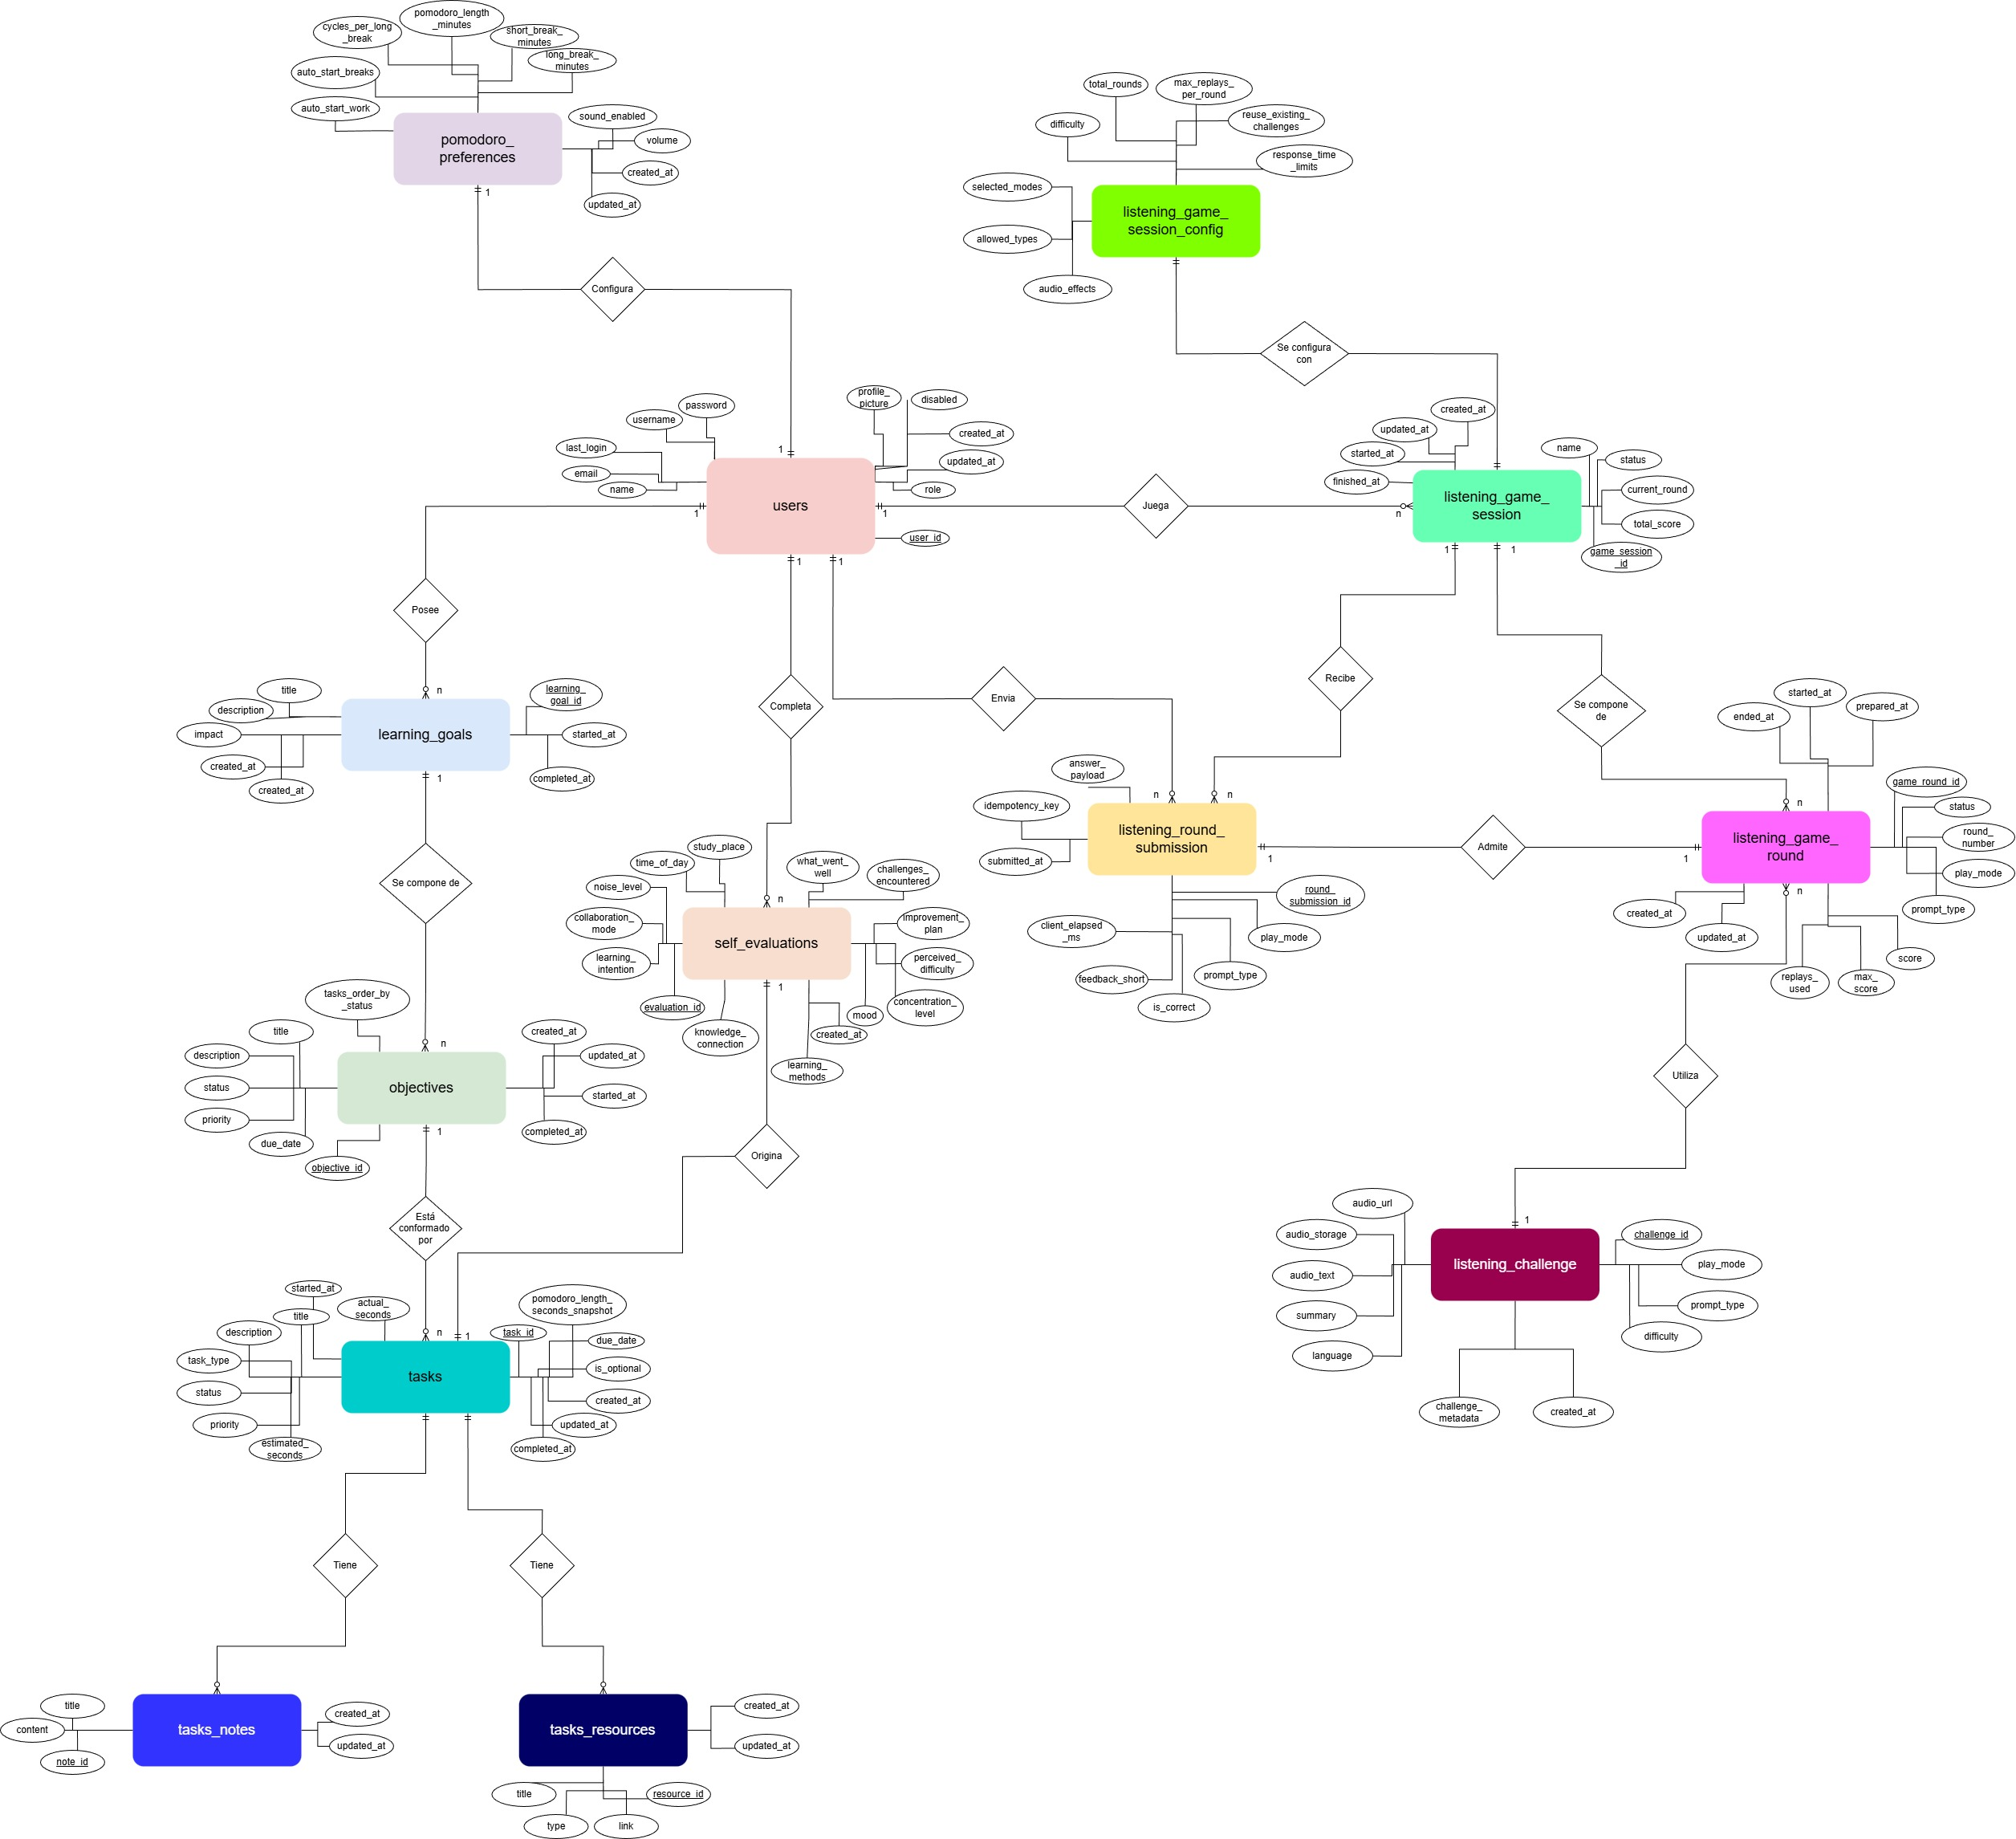
\includegraphics[width=\textwidth]{Figuras/mer_soft_skills_back.jpg} 
    \caption{Modelo entidad–relación. Elaboración propia.}
    \label{fig:erd}
\end{figure}



\subsubsection{Modelo documental (MongoDB)}

El modelo documental complementa al esquema relacional para aquellas funcionalidades que
requieren manejar estructuras jerárquicas completas o layouts visuales. En particular, se emplean
dos colecciones principales: \texttt{learning\_goals} y \texttt{roadmaps}, definidas en bases de datos
separadas para organizar la información persistida en el módulo de Aprender a Aprender y
en el editor de roadmaps.

\begin{itemize}
  \item \textbf{Colección \texttt{learning\_goals}}: almacena documentos que representan una meta
  de aprendizaje con toda su jerarquía de objetivos y tareas anidados. Cada documento replica la
  estructura lógica definida en PostgreSQL, incluyendo el orden de los objetivos y la organización de
  tareas por estado, lo que permite recuperar en una sola consulta la estructura completa que se
  muestra en la interfaz.

  \item \textbf{Colección \texttt{roadmaps}}: guarda los planes de aprendizaje generados y
  compartidos por los usuarios. Además de los objetivos y tareas, incorpora un campo de
  \textit{layout} que registra la posición de los nodos y las aristas del diagrama, permitiendo
  reconstruir la representación visual del roadmap en el editor, así como configurar su visibilidad
  (pública o privada) y la información del autor.
\end{itemize}

\subsubsection{Sincronización y decisiones de diseño}
MongoDB resulta adecuado para almacenar layouts visuales y estructuras jerárquicas que evolucionan
con frecuencia, mientras que PostgreSQL concentra los datos transaccionales del sistema (como
sesiones de juego, rondas, desafíos y envíos de respuestas) donde se requieren transacciones ACID,
restricciones de unicidad e integridad referencial.
\\
\\
Las operaciones de creación, actualización y eliminación sobre metas, objetivos y tareas se ejecutan
inicialmente en PostgreSQL y, de forma coordinada, se reflejan en MongoDB mediante servicios
especializados que serializan los modelos relacionales en documentos. Este esquema de
sincronización dual permite aprovechar las garantías del modelo relacional sin sacrificar la
eficiencia necesaria para recuperar estructuras completas en las visualizaciones del sistema.
\\
\\
La decisión de mantener una representación documental de \texttt{learning\_goals} en MongoDB,
además de su almacenamiento en PostgreSQL, responde a necesidades específicas del módulo
Aprender a Aprender. Las visualizaciones requieren obtener en una única operación la jerarquía
completa de una meta (objetivos, tareas, recursos y su organización tipo Kanban), lo que en un
modelo relacional implicaría múltiples uniones o consultas encadenadas. En MongoDB esta jerarquía
se conserva como un documento anidado, lo que permite su recuperación con baja latencia. 
\\
\\
Asimismo, mantener una representación documental de los planes accionables (\texttt{learning\_goals}) en MongoDB simplifica de manera significativa la conversión entre un roadmap y su versión operativa. Ambas
estructuras (el roadmap y el plan accionable) comparten un formato jerárquico anidado basado
en objetivos y tareas, lo que permite transformarlas entre sí sin necesidad de reconstruir relaciones
mediante consultas complejas.
\\
\\
En la conversión de un plan accionable hacia un roadmap, el sistema recupera desde MongoDB el
documento completo asociado, evitando múltiples consultas o uniones en PostgreSQL para
reconstruir la jerarquía. Dado que el roadmap también se almacena como un documento anidado,
la transformación consiste principalmente en reorganizar la misma estructura de datos para
adaptarla al editor visual.
\\
\\
En sentido inverso, cuando un usuario adopta un roadmap como plan de aprendizaje, el sistema
itera sobre sus objetivos y tareas y crea los registros correspondientes en PostgreSQL. Aunque este
proceso genera nuevas entidades relacionales, la estructura documental del roadmap facilita el
mapeo, pues su jerarquía coincide con la utilizada por los planes accionables almacenados en
MongoDB. Posteriormente, el servicio de sincronización actualiza la versión documental,
garantizando coherencia entre ambos modelos persistidos.
\\
\\
Finalmente, el uso de campos JSONB, arreglos ordenados e índices compuestos en PostgreSQL
(especialmente en entidades como \texttt{objectives}, \texttt{tasks} y \texttt{listening\_game\_round})
complementa el modelo documental al permitir almacenar configuraciones flexibles y optimizar
consultas comunes sobre combinaciones de columnas (por ejemplo, \texttt{objective\_id} y
\texttt{status}, o \texttt{session\_id} y \texttt{round\_number}). En conjunto, la complementariedad entre
PostgreSQL y MongoDB permite combinar integridad, flexibilidad y rendimiento en las operaciones
propias de los módulos de Aprender a Aprender y Escucha Activa.


\subsubsection{Modelos de datos y validaciones}

El backend representa la información persistida mediante tres tipos de estructuras:
\begin{enumerate}[label=(\roman*), leftmargin=*]
    \item Modelos ORM basados en \texttt{SQLModel} para las entidades gestionadas en PostgreSQL.
    \item Esquemas de validación definidos con \texttt{Pydantic} para las operaciones de la API REST. 
    \item Modelos \texttt{Pydantic} utilizados para representar documentos almacenados en MongoDB.
\end{enumerate}
Los modelos construidos con \texttt{SQLModel} (que combinan las capacidades de 
\texttt{SQLAlchemy} y \texttt{Pydantic}) definen la estructura interna de las entidades 
persistidas en PostgreSQL. Por su parte, los esquemas Pydantic complementan esta 
definición mediante validaciones adicionales aplicadas durante el intercambio de datos 
con la API. Entre los elementos más relevantes se encuentran:

\begin{itemize}
    \item \textbf{Modelos SQLModel}: definen campos tipados, relaciones mediante 
    \texttt{Relationship}, configuraciones de persistencia y validaciones básicas que 
    reflejan de manera directa el esquema relacional.
    
    \item \textbf{Esquemas Pydantic}: incorporan restricciones de formato, valores por 
    defecto y validaciones de negocio implementadas mediante 
    \texttt{@field\_validator}. También permiten aplicar serialización personalizada 
    mediante \texttt{@field\_serializer} y definir campos derivados con 
    \texttt{@computed\_field}.
    
    \item \textbf{Enumeraciones tipadas}: el backend utiliza \texttt{enums} para 
    representar estados, categorías, tipos de recurso y modos de interacción, 
    favoreciendo la estandarización del dominio y reduciendo errores en el flujo de 
    datos.
\end{itemize}

En la mayoría de los casos, los esquemas Pydantic heredan de clases base definidas con
\texttt{SQLModel} (por ejemplo, \texttt{TaskCreate(TaskBase)}), permitiendo reutilizar
atributos comunes y añadir validaciones específicas para las operaciones de creación,
actualización o respuesta. Estos esquemas también incluyen ejemplos de uso mediante
\texttt{json\_schema\_extra}, que se integran con la documentación OpenAPI generada
automáticamente por FastAPI. Para formatos de respuesta homogéneos, se emplean
estructuras genéricas como \texttt{BaseResponse[T]} y \texttt{PaginatedResponse[T]},
las cuales facilitan la consistencia del diseño y refuerzan el tipado estático en el
intercambio de datos.
\\
\\
Este diseño favorece el desacoplamiento entre la representación interna de los datos y su persistencia, asegurando que las operaciones de la API manipulen información válida, coherente y consistente con las reglas definidas para el funcionamiento del sistema.

\subsection{Diseño de la API REST}

La API REST del sistema se estructura bajo principios arquitectónicos orientados a recursos, con un diseño modular que facilita la extensibilidad, la mantenibilidad y la separación clara de responsabilidades. Todas las rutas siguen convenciones consistentes relativas al uso de sustantivos en plural, versionamiento mediante el prefijo \texttt{/api/v1}, verbos HTTP con semántica estándar (GET, POST, PATCH, DELETE) y representación jerárquica de subrecursos cuando la relación entre entidades así lo requiere.

\paragraph{Estilo y convenciones RESTful.}
La definición de endpoints sigue un enfoque RESTful pragmático: se emplean rutas basadas en
recursos para operaciones CRUD, mientras que las acciones especializadas del dominio se expresan como endpoints orientados a comandos, por ejemplo: \texttt{/game-sessions/\{id\}/start}, \texttt{/tasks/\{id\}/status} o \texttt{/roadmaps/\{id\}/publish}. Esta estrategia permite mantener un equilibrio entre claridad semántica y expresividad del dominio.

\paragraph{Estructura modular de routers.}
La API se organiza en routers independientes que representan dominios funcionales del sistema: \textit{autenticación y usuarios}, \textit{Aprender a Aprender} (metas, objetivos, tareas, notas, recursos y autoevaluaciones), \textit{Escucha Activa} (sesiones, rondas, desafíos y generación de audio), \textit{roadmaps} y \textit{módulos del sistema}. Cada router encapsula las rutas de su dominio y se agrupa en la documentación OpenAPI mediante etiquetas específicas, lo que facilita su navegación y comprensión.

\paragraph{Contratos de intercambio de datos.}
El intercambio entre cliente y servidor se realiza mediante esquemas \texttt{Pydantic} que definen la estructura de las solicitudes y respuestas. Estos incluyen:
\begin{itemize}
    \item \textbf{Schemas de creación} (\texttt{*Create}), basados en clases modelo con campos mínimos requeridos.
    \item \textbf{Schemas de actualización} (\texttt{*Update}), que permiten modificaciones parciales.
    \item \textbf{Schemas de lectura} (\texttt{*Read}), con serializadores personalizados, campos derivados y formateo especializado.
    \item \textbf{Wrappers genéricos} como \texttt{BaseResponse[T]} y \texttt{PaginatedResponse[T]}, utilizados para estandarizar respuestas y soportar tipado fuerte.
\end{itemize}
La separación entre modelos internos de persistencia y esquemas expuestos en la API reduce el
acoplamiento y facilita la evolución del sistema.

\paragraph{Autenticación, autorización y seguridad.}
La API implementa autenticación mediante tokens JWT, que son verificados a través de
dependencias que validan firma, expiración e identidad del usuario. Todas las operaciones (con
excepción del registro e inicio de sesión) requieren autenticación previa. La autorización se
gestiona mediante validaciones de propiedad de los recursos, reglas basadas en roles y servicios que
encapsulan las restricciones de negocio y generan excepciones adecuadas (\textit{Forbidden},
\textit{Conflict}, \textit{Missing}, entre otras).

\paragraph{Manejo de errores y códigos de estado.}
Las excepciones personalizadas se traducen a respuestas HTTP con una estructura uniforme que
incluye un título y un mensaje descriptivo. El backend emplea un conjunto consistente de códigos
de estado, entre los cuales se destacan:

\begin{itemize}
    \item \textbf{200 / 201} — Operaciones exitosas (consulta y creación de recursos).
    \item \textbf{400 / 422} — Errores de validación o datos de entrada inválidos.
    \item \textbf{401} — Credenciales inválidas o no proporcionadas.
    \item \textbf{403} — Acción no permitida para el usuario autenticado.
    \item \textbf{404} — Recurso no encontrado.
    \item \textbf{409} — Conflictos en la operación (por ejemplo, restricciones de unicidad o estados incompatibles).
    \item \textbf{423} — Recurso bloqueado o no disponible temporalmente.
    \item \textbf{500} — Error interno inesperado.
\end{itemize}

\paragraph{Paginación, filtros y parámetros de búsqueda.}
La API ofrece paginación estándar mediante \texttt{offset} y \texttt{limit}, así como filtros
especializados por dominio:
\begin{itemize}
    \item Estado, prioridad y búsqueda por texto para tareas.
    \item Filtros por título, autor, visibilidad y número de pasos en el caso de los roadmaps.
    \item Criterios de ordenamiento y filtrado para autoevaluaciones.
\end{itemize}
Este enfoque permite obtener consultas eficientes, adaptadas a las necesidades del usuario.

\paragraph{Versionamiento y documentación automática.}
Toda la API está versionada bajo el prefijo \texttt{/api/v1}, facilitando su evolución sin afectar
integraciones existentes. La documentación se genera automáticamente mediante OpenAPI e incluye
ejemplos, descripciones detalladas y una agrupación clara por dominios funcionales, accesible a
través de Swagger UI y ReDoc.

\paragraph{Decisiones de diseño relevantes.}
Entre las decisiones más importantes se encuentran:
\begin{itemize}
    \item Routers que actúan únicamente como capa de orquestación, delegando el procesamiento a servicios especializados.
    \item Uso sistemático de inyección de dependencias para sesiones de base de datos y autenticación.
    \item Validación en múltiples capas (formato en \texttt{Pydantic} y reglas de negocio en servicios).
    \item Inclusión de endpoints orientados a acción cuando el dominio lo requiere.
    \item Utilización de tareas en segundo plano para operaciones de alto costo (por ejemplo, preparación anticipada de rondas en el módulo de Escucha Activa).
    \item Rutas jerárquicas que reflejan relaciones naturales del dominio, como sesiones de juego y sus rondas asociadas.
\end{itemize}

\subsection{Endpoints principales}

La API REST expone un conjunto de endpoints organizados por dominios funcionales,
cada uno orientado a cubrir las operaciones necesarias para el uso de los módulos del
prototipo. Estos dominios agrupan las rutas según las actividades que gestionan, lo
que facilita su consulta y estructura la interacción entre el cliente y el backend.
\\
\\
De manera general, los endpoints del sistema se concentran en las siguientes áreas:

\begin{itemize}
    \item \textbf{Autenticación y usuarios}: gestión del acceso, administración del perfil e
    interacción con preferencias asociadas al usuario.

    \item \textbf{Metas, objetivos y tareas}: operaciones para crear, consultar, modificar y
    eliminar planes accionables del módulo \textit{Aprender a Aprender}.

    \item \textbf{Notas, recursos y autoevaluaciones}: funcionalidades de apoyo que enriquecen
    el seguimiento del aprendizaje mediante comentarios, materiales externos y registros
    reflexivos.

    \item \textbf{Sesiones de Escucha Activa}: manejo completo del ciclo de juego, incluyendo
    creación de sesiones, avance entre rondas, envío de respuestas y consulta de resultados.

    \item \textbf{Desafíos de escucha}: generación de contenido auditivo mediante modelos de
    lenguaje y obtención del audio sintetizado asociado a cada desafío.

    \item \textbf{Roadmaps}: creación, edición y visualización de planes de aprendizaje en
    formato gráfico, así como su conversión hacia o desde metas de aprendizaje.

    \item \textbf{Administración de módulos}: operaciones destinadas a gestionar los módulos
    disponibles dentro de la plataforma.
\end{itemize}

La especificación completa de cada endpoint, incluyendo parámetros, cuerpos de
solicitud y respuesta, códigos de estado y ejemplos detallados, se encuentra
disponible en el \hyperref[anexo:endpoints]{\textbf{Anexo H}}.
\section{Desarrollo del frontend}

\subsection{Configuración del entorno}

Para la implementación del frontend se empleó \textit{Vite} como entorno de construcción del proyecto, utilizando la plantilla con soporte para \textit{TypeScript} con el fin de garantizar un desarrollo tipado, estructurado y escalable. Sobre esta base se definieron las configuraciones iniciales del proyecto, entre ellas:

\begin{itemize}
    \item \textbf{React como biblioteca base:} instalada desde la configuración inicial del proyecto para gestionar la creación y composición de los componentes que conforman la interfaz.

    \item \textbf{Tema global con Material UI (MUI):} configurado mediante su proveedor de estilos para unificar criterios de color, tipografía y lineamientos visuales desde el arranque de la aplicación.

    \item \textbf{Internacionalización con i18next:} cargado en la inicialización del proyecto para habilitar soporte multilenguaje y permitir la gestión flexible de textos traducibles.

    \item \textbf{React Query como proveedor global:} utilizado para manejar el estado de las solicitudes a la API, el manejo del \textit{cache} y los estados de carga de manera centralizada.

    \item \textbf{ESLint como herramienta de análisis estático:} configurada para asegurar buenas prácticas, detectar errores comunes y mantener la consistencia del código durante el desarrollo.

    \item \textbf{Variables de entorno administradas mediante Vite:} empleadas para parametrizar valores como las URLs de los servicios del backend y facilitar la ejecución del prototipo en entornos diferenciados.
\end{itemize}

En conjunto, estas configuraciones establecieron una base sólida y organizada que permitió desarrollar el frontend de manera estable, modular y coherente.

\subsection{Arquitectura y organización}

\subsubsection{Enfoque arquitectónico general}
El frontend del prototipo se desarrolló siguiendo una arquitectura basada en componentes y organizada bajo un enfoque modular por características (\textit{feature-based}). Este enfoque agrupa dentro de cada módulo todos los elementos necesarios para una funcionalidad específica, tales como componentes visuales, vistas, servicios de comunicación, estados globales y funciones auxiliares. Esta organización permitió mantener una separación clara de responsabilidades, mejorar la cohesión interna de cada módulo y facilitar la evolución independiente de las diferentes partes del sistema.

\subsubsection{Organización modular por funcionalidades}
La aplicación se estructura en módulos que corresponden a las funcionalidades principales del prototipo, entre ellos el módulo de \textit{Aprender a Aprender}, el módulo de \textit{Escucha Activa} y el módulo de autenticación. Esta distribución permite organizar las funcionalidades en segmentos claramente delimitados, cada uno con su propio conjunto de elementos y flujos asociados.

\begin{figure}[H]
\centering
\begin{verbatim}
frontend/
|-- public/                       (Archivos estáticos accesibles públicamente)
|-- src/
|   |-- api/                      (Clientes y funciones para consumir el backend)
|   |-- app/                      (Configuración global de la aplicación, rutas y layout)
|   |-- assets/                   (Recursos gráficos y multimedia)
|   |-- components/               (Componentes reutilizables de la interfaz)
|   |-- config/                   (Configuración de clientes API, constantes globales y variables de entorno)
|   |-- features/
|   |   |-- active-listening/     (Módulo de Escucha Activa)
|   |   |   |-- api/              (Llamadas específicas del módulo al backend)
|   |   |   |-- assets/           (Iconos, sonidos e imágenes del módulo)
|   |   |   |-- components/       (Componentes UI propios del módulo)
|   |   |   |-- constants/        (Constantes y parámetros usados en el juego)
|   |   |   |-- pages/            (Páginas del módulo)
|   |   |   |-- store/            (Estados y acciones en Zustand para el módulo)
|   |   |   |-- types/            (Tipos y modelos TypeScript del módulo)
|   |   |   +-- utils/            (Funciones auxiliares internas)
|   |   |
|   |   |-- authentication/       (Autenticación: login, registro, recuperación)
|   |   +-- learn-to-learn/       (Módulo Aprender a Aprender)
|   |
|   +-- ...
+-- ...
\end{verbatim}
\caption{Estructura de carpetas del frontend organizada por características (\textit{feature-based}). Elaboración propia.}
\label{fig:frontend-feature-structure}
\end{figure}


\subsubsection{Sistema de enrutamiento y uso de layouts}
La navegación de la interfaz se gestiona mediante un sistema de enrutamiento que organiza las rutas principales del frontend e incorpora distintos \textit{layouts} para estructurar grupos de vistas relacionadas. Estos \textit{layouts} actúan como contenedores que reúnen elementos compartidos, tales como barras de navegación, encabezados o paneles laterales, y permiten definir la disposición general de cada sección. De esta manera, el enrutamiento establece la jerarquía visual y funcional del frontend, articulando la relación entre las diferentes vistas que conforman cada módulo.

\subsubsection{Diseño de componentes}
En el diseño de componentes se adoptó una aproximación que distingue entre componentes presentacionales y componentes contenedores, aunque con un grado de flexibilidad práctica. Los componentes presentacionales se centran principalmente en la representación visual y la interacción básica, recibiendo datos y funciones a través de \textit{props}. No obstante, en algunos casos estos componentes acceden directamente a estados globales cuando resulta más eficiente que propagar múltiples propiedades desde niveles superiores. Por su parte, los componentes contenedores se encargan de coordinar la interacción del usuario, gestionar la comunicación con los estados globales y organizar los flujos relacionados con servicios externos. Este enfoque híbrido permitió distribuir responsabilidades de manera equilibrada, mantener la coherencia de la interfaz y facilitar la reutilización de componentes en distintos contextos del sistema.

\subsubsection{Gestión del estado global y datos asincrónicos}
La gestión del estado global se implementó mediante un conjunto de almacenes especializados organizados por módulo, lo que permitió centralizar la información relevante y mantener una estructura coherente para el acceso y actualización del estado. Estos almacenes incorporan mecanismos que facilitan la trazabilidad de cambios y la manipulación inmutable de los datos. Por su parte, la gestión de datos asincrónicos provenientes del servidor se realizó mediante una herramienta dedicada al control del almacenamiento en caché, la revalidación y la sincronización controlada con la API, lo que permitió reducir solicitudes redundantes y asegurar la consistencia entre la interfaz y el estado persistente del sistema.

\subsubsection{Funciones reutilizables y lógica transversal}
Finalmente, la arquitectura del frontend integra un conjunto de funciones reutilizables que encapsulan lógica transversal, tales como validaciones, transformaciones de datos y operaciones comunes a varios módulos. Estas funciones contribuyen a la mantenibilidad del código, evitan la duplicación de lógica y favorecen la coherencia en la implementación de los distintos componentes del sistema.

\subsection{Componentes principales}

En esta sección se describen los componentes de interfaz más relevantes del frontend, organizados según los módulos funcionales del prototipo. Estos componentes constituyen los elementos centrales de interacción del usuario y articulan las principales operaciones de cada módulo.

\subsubsection{Módulo \textit{Learn to Learn}}

El módulo de \textit{Learn to Learn} integra una serie de componentes que permiten gestionar metas de aprendizaje, objetivos, tareas y su representación visual mediante \textit{roadmaps}. En la Tabla~\ref{tab:componentes-learn-to-learn} se presentan los componentes principales y su rol dentro del prototipo.

\begin{table}[H]
\centering
\footnotesize
\begin{tabular}{| m{3.5cm} | m{11cm} |}
\hline
\textbf{Componente} & \textbf{Rol funcional en el prototipo} \\
\hline
\textit{RoadmapEditor} & Componente central del módulo, encargado de orquestar la construcción y edición de \textit{roadmaps} de aprendizaje. Gestiona la interacción con la representación gráfica, la disposición de los nodos y las acciones asociadas al proceso de edición. \\
\hline
\textit{ObjectiveNode} & Representa visualmente un objetivo dentro del \textit{roadmap}. Permite identificar, seleccionar y manipular objetivos individuales, sirviendo como unidad básica de la estructura gráfica del plan de aprendizaje. \\
\hline
\textit{TaskCard} / \textit{TaskNode} & Componente utilizado para mostrar y gestionar las tareas asociadas a un objetivo, integrando información relevante (descripción, estado, estimaciones) y las acciones principales de seguimiento. \\
\hline
\textit{Board} & Tablero Kanban encargado de estructurar la visualización de las tareas según su estado (por ejemplo, pendiente, en progreso o completada). Facilita la organización y el seguimiento del avance del estudiante. \\
\hline
\textit{GoalsSection} & Vista principal de las metas de aprendizaje, desde la cual el usuario accede a la creación, consulta y administración de objetivos, así como a la navegación hacia el editor de \textit{roadmaps} y otras funcionalidades relacionadas. \\
\hline
\end{tabular}
\caption{Componentes principales del módulo \textit{Learn to Learn}.}
\label{tab:componentes-learn-to-learn}
\end{table}

\subsubsection{Módulo de \textit{Escucha Activa}}

El módulo de \textit{Escucha Activa} se centra en la realización de sesiones de práctica auditiva mediante modos de juego que combinan reproducción de audio, resolución de desafíos y retroalimentación. La Tabla~\ref{tab:componentes-escucha-activa} resume los componentes principales que intervienen en este flujo.

\begin{table}[H]
\centering
\footnotesize
\begin{tabular}{| m{3.5cm} | m{11cm} |}
\hline
\textbf{Componente} & \textbf{Rol funcional en el prototipo} \\
\hline
\textit{GameSessionForm} & Formulario empleado para configurar una sesión de práctica, incluyendo la selección del modo de juego y los parámetros necesarios antes de iniciar el ejercicio auditivo. \\
\hline
\textit{GamePlay} & Componente central del módulo, encargado de coordinar el flujo completo de la sesión de juego: carga del desafío auditivo, gestión de rondas, recepción de respuestas y transición entre etapas de la actividad. \\
\hline
\textit{AudioPlayer} & Componente dedicado a la reproducción del audio del desafío, ofreciendo controles básicos de interacción (reproducir, pausar, reiniciar) y garantizando una experiencia de escucha clara y controlada. \\
\hline
\textit{GameModeContent} & Panel de respuesta que se adapta al modo de juego seleccionado (por ejemplo, \textit{Focus}, \textit{Cloze}, \textit{Paraphrase}, \textit{Summarize}, \textit{Clarify}), permitiendo al usuario registrar su respuesta según la dinámica del ejercicio. \\
\hline
\textit{GameSessionResult} / \textit{ScoreSummary} & Vista que presenta el resultado final de la sesión e integra un componente especializado para resumir el desempeño del usuario, mostrar la retroalimentación generada y ofrecer una visión consolidada de la actividad realizada. \\
\hline
\end{tabular}
\caption{Componentes principales del módulo de \textit{Escucha Activa}.}
\label{tab:componentes-escucha-activa}
\end{table}

\subsection{Gestión del estado y comunicación con la API}

El frontend del prototipo requiere una gestión cuidadosa del estado y una comunicación fluida con la API para soportar las funcionalidades interactivas de los módulos. La necesidad de estado global surge de la naturaleza modular del sistema, en la que distintos componentes y vistas comparten información contextual, como la sesión de juego activa, el \textit{roadmap} en edición o las notificaciones del sistema. Asimismo, el prototipo maneja datos dinámicos que se actualizan de manera continua durante la interacción del usuario, tales como el progreso en una ronda de escucha activa, la posición de nodos en el editor o el estado de carga de determinadas secciones.
\\
\\
La sincronización con la API es fundamental para mantener la coherencia entre el estado local y los datos persistentes en el servidor, especialmente en operaciones como el auto-guardado del editor de \textit{roadmaps}, la actualización de tareas en el tablero Kanban o la obtención de resultados de sesiones de juego. Finalmente, el soporte para módulos independientes exige que cada uno gestione su propio estado de manera aislada, minimizando dependencias y favoreciendo la escalabilidad del sistema.

\subsubsection{Gestión del estado global con Zustand}

La gestión del estado global se implementó mediante \textit{Zustand}, una librería ligera que ofrece una API sencilla, baja sobrecarga y una organización modular a través de \textit{stores} independientes. Cada módulo cuenta con su propio store especializado lo que permite que cada funcionalidad evolucione sin afectar al resto de la aplicación.
\\
\\
Adicionalmente, se configuró un store transversal para funcionalidades compartidas, como el sistema de notificaciones globales. Para mejorar la experiencia de desarrollo y garantizar la inmutabilidad del estado, se integraron dos middlewares: uno para herramientas de desarrollo, que permite inspeccionar y rastrear cambios, y otro para manipulación inmutable mediante escritura declarativa.
\\
\\
Este enfoque aporta trazabilidad durante el desarrollo, asegura un manejo seguro del estado y mantiene una organización coherente entre las distintas funcionalidades, lo que facilita la comprensión y el mantenimiento del código.

\subsubsection{Comunicación con la API mediante React Query}

La comunicación con el servidor se gestionó mediante \textit{React Query}, una librería especializada en administración de datos asincrónicos que proporciona almacenamiento en caché, revalidación inteligente y sincronización controlada con la API. El sistema de caché evita solicitudes redundantes y mejora el rendimiento, mientras que la revalidación automática garantiza que la interfaz muestre siempre la información más actualizada disponible sin interrumpir la experiencia del usuario.
\\
\\
La librería permite compartir de forma automática los datos entre componentes que dependen de los mismos recursos del backend, evitando duplicaciones innecesarias. Además, su política de reintentos facilita la recuperación ante fallos temporales de red. La integración con el ciclo de vida de los componentes se realizó mediante \textit{hooks} personalizados que encapsulan la lógica de consulta y mutación, permitiendo un consumo declarativo de los datos y manejando de forma automática estados de carga, error y éxito.
\\
\\
En el módulo Learn to Learn, por ejemplo, la lista de metas, objetivos y tareas se mantiene sincronizada mediante invalidación de queries y actualizaciones optimistas, lo que permite que los cambios realizados por el usuario se reflejen inmediatamente en la interfaz, incluso antes de recibir la confirmación del servidor.

\subsubsection{Integración entre stores y React Query}

La arquitectura del prototipo establece una separación clara entre estado de interfaz y estado persistente. \textit{Zustand} se utiliza para almacenar estados transitorios relacionados con la interacción del usuario (como el nodo seleccionado en el editor, la ronda actual del juego o estados de visibilidad del UI) mientras que \textit{React Query} administra datos provenientes del servidor, como metas, objetivos, tareas o resultados de sesiones de juego.
\\
\\
La interacción entre ambos sistemas se manifiesta en flujos en los cuales el usuario mantiene un contexto local mientras la aplicación sincroniza datos persistentes. Por ejemplo, al seleccionar un objetivo, el identificador correspondiente se almacena en un store, mientras que las tareas asociadas se obtienen mediante React Query, aprovechando la caché si los datos ya fueron recuperados previamente. En el editor de roadmaps, los datos del grafo se mantienen en un store para permitir manipulaciones inmediatas, mientras que la persistencia se gestiona mediante mutaciones que, al completarse, invalidan las consultas relacionadas para mantener la coherencia con otras vistas del sistema.

\subsubsection{Ventajas del enfoque combinado}

La combinación de Zustand y React Query aportó una base sólida para la implementación del frontend. La modularidad derivada de los stores independientes facilita la evolución y el mantenimiento de cada funcionalidad. El sistema de caché de React Query reduce la carga sobre el servidor y evita duplicar solicitudes. La separación explícita entre estado local y estado persistente mejora la claridad conceptual y la estabilidad del sistema.




\section{Repositorios}

Los repositorios utilizados para el desarrollo del prototipo se encuentran disponibles en GitHub. El primero corresponde a la plataforma de habilidades blandas, que integra el backend desarrollado en FastAPI con SQLModel y el frontend construido en React. El segundo repositorio corresponde al agente Aithena basado en LangGraph, empleado para la generación guiada de roadmaps personalizados.

\medskip

\textbf{Repositorio de la plataforma:}\\
\href{https://github.com/Paoladevelopment/soft-skills-plataform}{\texttt{https://github.com/Paoladevelopment/soft-skills-plataform}}

\medskip

\textbf{Repositorio del agente Aithena:}\\
\href{https://github.com/Paoladevelopment/aithena-roadmap-generation-agent}{\texttt{https://github.com/Paoladevelopment/aithena-roadmap-generation-agent}}





%%%%%%%%%%%%%%%%%%%%%%%%%%%%%%Capitulo 8%%%%%%%%%%%
\chapter{Pruebas sobre el prototipo}
\markboth{Pruebas sobre el prototipo}{Pruebas sobre el prototipo}
El presente capítulo expone la evaluación piloto del prototipo desarrollado, en correspondencia con el \textbf{Objetivo Específico 5}, orientado a:

\begin{quote}
Evaluar la efectividad de los módulos en términos de comprensión del contenido, participación, motivación, retención de información y aplicación práctica, mediante pruebas piloto y retroalimentación de los estudiantes, identificando áreas de mejora.
\end{quote}

Para ello se aplicaron tres encuestas dirigidas a estudiantes de Ingeniería de Sistemas, cuyos resultados permiten analizar los criterios de evaluación definidos en este objetivo.
\\
\\
Con el propósito de mantener el capítulo enfocado en el análisis, se presenta aquí una síntesis estructurada de los hallazgos, mientras que la evidencia detallada (preguntas, respuestas completas y gráficos por pregunta) se incluye en el \hyperref[anexo:encuestas]{Anexo I}.

\section{Justificación de las pruebas}

La aplicación de pruebas a los estudiantes es fundamental para determinar en qué medida el prototipo contribuye al desarrollo de las habilidades blandas trabajadas en este proyecto. En particular, las encuestas permiten:

\begin{itemize}
    \item Obtener información directa sobre la experiencia de los estudiantes con los módulos.
    \item Identificar fortalezas, dificultades y oportunidades de mejora desde la perspectiva de los estudiantes.
    \item Validar el diseño del prototipo y comprender su impacto formativo.
    \item Orientar ajustes futuros para optimizar la experiencia de aprendizaje.
\end{itemize}

\section{Metodología de aplicación}

El proceso de evaluación del prototipo se desarrolló con dos poblaciones objetivo diferenciadas, con el fin de obtener perspectivas complementarias sobre la usabilidad de la plataforma y la efectividad percibida de los módulos formativos.

\subsection*{Población 1: Evaluación de usabilidad (Heurísticas de Nielsen)}
\begin{itemize}
    \item \textbf{Población objetivo:} Egresados y profesionales de Ingeniería de Sistemas.
    
    \item \textbf{Justificación:} Esta población cuenta con experiencia técnica y criterio profesional para evaluar la interfaz con mayor profundidad, lo que facilita identificar problemas de usabilidad, consistencia y diseño que pueden pasar desapercibidos para los usuarios finales.
    
    \item \textbf{Enfoque:} Aplicación de una encuesta construida a partir de las heurísticas de Nielsen, adaptadas al contexto educativo.
\end{itemize}

\subsection*{Población 2: Evaluación de efectividad percibida (usuarios finales)}
\begin{itemize}
    \item \textbf{Población objetivo:} Estudiantes de Ingeniería de Sistemas, usuarios finales del prototipo.
    
    \item \textbf{Justificación:} La participación de los estudiantes es fundamental, puesto que el prototipo fue diseñado para apoyar su proceso de aprendizaje y solo ellos pueden ofrecer una valoración basada en su propia experiencia de uso.
    
    \item \textbf{Enfoque:} Aplicación de dos encuestas centradas en los módulos específicos Aprender a Aprender y Escucha Activa.
\end{itemize}

\section{Descripción de las encuestas aplicadas}

A continuación se describen los tres instrumentos utilizados en la evaluación del prototipo. Todas las encuestas combinaron preguntas cerradas tipo Likert con preguntas abiertas, lo que permitió obtener tanto valoraciones cuantitativas como observaciones cualitativas sobre el funcionamiento de los módulos y la experiencia de uso de la plataforma.


\begin{itemize}
    \item \textbf{Encuesta 1: Evaluación del módulo Aprender a Aprender.}  
    Instrumento orientado a identificar cómo los estudiantes comprendieron los componentes centrales del módulo (metas, objetivos, tareas y roadmap), así como la utilidad percibida de las herramientas implementadas (tablero Kanban, editor visual de roadmaps y autoevaluaciones).
    La encuesta recoge percepciones sobre claridad, participación, motivación, retención de conceptos clave y aplicación práctica, complementadas con preguntas abiertas que permiten identificar experiencias, dificultades y sugerencias.


    \item \textbf{Encuesta 2: Evaluación del módulo Escucha Activa.}  
    Instrumento diseñado para valorar la experiencia de los estudiantes con las actividades auditivas del módulo y su contribución al desarrollo de habilidades de escucha activa.
    Evalúa la comprensión de los principios trabajados, la utilidad de la retroalimentación, la capacidad para recordar información, y la aplicabilidad de lo aprendido en contextos reales.
    Incluye además preguntas abiertas que permiten identificar audios más útiles, dificultades frecuentes y recomendaciones de mejora.


    \item \textbf{Encuesta 3: Evaluación de usabilidad de la plataforma.}  
    
    Instrumento dirigido a valorar la usabilidad del prototipo tomando como referencia las heurísticas de Nielsen. La encuesta incluye ítems destinados a medir la claridad del estado del sistema, la consistencia de la interfaz, la facilidad de navegación, la prevención de errores y la comprensión de mensajes e indicadores visuales. 
    
    Complementariamente, incorpora preguntas abiertas orientadas a identificar elementos confusos, dificultades de uso y sugerencias de mejora relacionadas con la experiencia general de usuario.

\end{itemize}

\section{Proceso de aplicación}

La recolección de información se desarrolló mediante un procedimiento mixto que combinó momentos de aplicación guiada con participación asincrónica. Cada encuesta fue distribuida según la población objetivo correspondiente, junto con una breve explicación del propósito del estudio y las instrucciones para su diligenciamiento.
\\
\\
En el caso de la evaluación de usabilidad, el enlace fue compartido con egresados y profesionales de Ingeniería de Sistemas, quienes exploraron libremente el prototipo antes de completar la encuesta basada en las heurísticas de Nielsen.
\\
\\
Para la evaluación de los módulos \textit{Aprender a Aprender} y \textit{Escucha Activa}, se contó con la colaboración de un docente del programa, quien facilitó un espacio presencial de aproximadamente 30 minutos en el que los estudiantes interactuaron con el prototipo y posteriormente diligenciaron las encuestas correspondientes. Este espacio permitió asegurar que todos los participantes tuvieran un primer acercamiento guiado al funcionamiento del sistema.
\\
\\
Adicionalmente, se ofreció la posibilidad de responder las encuestas de manera asincrónica para aquellos estudiantes que no lograron completar el formulario durante el espacio asignado. Con ello se garantizó la participación de un mayor número de estudiantes y se respetaron sus tiempos individuales.


\section{Limitaciones del proceso de evaluación}

Si bien las encuestas aplicadas permitieron obtener información valiosa sobre la experiencia de uso y la efectividad percibida del prototipo, el proceso de evaluación presenta algunas limitaciones que deben considerarse al interpretar los resultados.

\begin{itemize}
    \item \textbf{Alcance exploratorio:} La evaluación corresponde a una fase temprana de validación del prototipo, lo que implica que los resultados se enfocan en percepciones y no permiten establecer conclusiones causales sobre el desarrollo de habilidades.

    \item \textbf{Tamaño y composición de la muestra:} La participación estuvo limitada a estudiantes y egresados disponibles durante el periodo de aplicación, lo que reduce la posibilidad de generalizar los resultados a toda la población estudiantil.

    \item \textbf{Tiempo de interacción con el prototipo:} Aunque se contó con un espacio guiado de 30 minutos, este tiempo puede no haber sido suficiente para explorar en profundidad todas las funcionalidades, especialmente en el módulo \textit{Aprender a Aprender}, que involucra procesos más prolongados.

    \item \textbf{Autorreporte:} Al basarse en encuestas, los resultados dependen de la autorreflexión y percepción subjetiva de los participantes, lo cual puede introducir sesgos asociados a expectativas, motivación u otros factores personales.

    \item \textbf{Necesidad de experiencia sostenida:} Algunos componentes del prototipo, como la construcción de hábitos o la planificación a largo plazo, requieren un uso continuo que no pudo evaluarse en el marco de una sesión breve.

    \item \textbf{Ausencia de grupo control:} No se incluyó un grupo que no utilizara el prototipo, por lo que no fue posible realizar comparaciones.
\end{itemize}

Estas limitaciones no invalidan los hallazgos obtenidos; más bien permiten contextualizar su alcance y abren la puerta a futuras investigaciones y evaluaciones más amplias.







\section{Resultados y análisis}

\subsection{Resultados de la Encuesta 1: Módulo \textit{Aprender a Aprender}}

Los resultados presentados a continuación se basan en las 38 respuestas recopiladas. Las tablas completas con los promedios por ítem y el número de respuestas se encuentran en el \hyperref[anexo:encuestas]{Anexo I} (véanse Tablas~\ref{tab:anexo-aaa-comprension} a~\ref{tab:anexo-aaa-aplicacion}).

\subsubsection*{Comprensión y uso de las herramientas del módulo}

Los datos muestran que los estudiantes comprendieron adecuadamente la estructura del módulo y el funcionamiento de sus principales herramientas. Los promedios por ítem se ubicaron en valores altos de la escala Likert (entre 4.00 y 4.39), lo que indica claridad en el uso de las metas de aprendizaje, la relación entre objetivos y tareas, el tablero Kanban, el roadmap generado por el chatbot y las autoevaluaciones (véase Tabla~\ref{tab:anexo-aaa-comprension} en el \hyperref[anexo:encuestas]{Anexo I}).

\subsubsection*{Motivación y participación}

Las actividades del módulo generaron niveles favorables de motivación y participación, con promedios que oscilaron entre 4.13 y 4.42. Elementos como el tablero Kanban, la personalización de tareas, el editor visual de roadmaps y la interacción con el chatbot fueron percibidos como factores que favorecieron el involucramiento activo durante la experiencia de uso (véase Tabla~\ref{tab:anexo-aaa-motivacion} en el \hyperref[anexo:encuestas]{Anexo I}).

\subsubsection*{Aplicación práctica y retención de la información}

Los estudiantes reportaron que el módulo apoyó la retención de conceptos clave relacionados con la planificación, la autorregulación y la organización del aprendizaje. Los promedios de esta dimensión se situaron entre 4.08 y 4.54, destacándose la afirmación sobre la aplicabilidad de los contenidos en situaciones reales como el ítem con mayor valoración. Esto sugiere que los conocimientos adquiridos pueden transferirse a contextos académicos y personales (véase Tabla~\ref{tab:anexo-aaa-aplicacion} en el \hyperref[anexo:encuestas]{Anexo I}).

\vspace{0.4cm}

\subsection{Resultados de la Encuesta 2: Módulo \textit{Escucha Activa}}

Los resultados presentados a continuación se basan en las 25 respuestas recopiladas. Las tablas completas con los promedios por ítem, resultados dicotómicos y número de respuestas se encuentran en el \hyperref[anexo:encuestas]{Anexo I} (véanse Tablas~\ref{tab:anexo-ea-comprension} a~\ref{tab:anexo-ea-global}).

\subsubsection*{Comprensión del contenido}

Los ítems asociados a la comprensión de los principios de la escucha activa mostraron valoraciones altas, especialmente en relación con la identificación de ideas principales y la aplicación de la habilidad en situaciones reales. Los promedios se ubicaron entre 4.64 y 4.80 en la escala Likert, lo que indica que las explicaciones y la retroalimentación ofrecidas por el módulo fueron percibidas como claras y útiles (véase Tabla~\ref{tab:anexo-ea-comprension} en el \hyperref[anexo:encuestas]{Anexo I}).

\subsubsection*{Motivación y participación}

Las dinámicas del módulo, que incluyen la variedad de modos de juego, la estructura por rondas, el sistema de puntajes y la posibilidad de repetir el audio, favorecieron la motivación y el involucramiento activo de los estudiantes. Los promedios oscilaron entre 4.44 y 4.72, lo que refleja que las actividades fueron percibidas como dinámicas e interesantes y que mantuvieron la atención durante las sesiones de juego (véase Tabla~\ref{tab:anexo-ea-motivacion} en el \hyperref[anexo:encuestas]{Anexo I}).

\subsubsection*{Retención de la información}

La mayoría de los estudiantes señaló haber mejorado su capacidad para recordar detalles importantes después de escuchar los audios: el 92\,\% indicó una percepción positiva de mejora y solo el 8\,\% manifestó lo contrario. Adicionalmente, la diversidad de estilos de contenido y niveles de dificultad fue valorada con un promedio de 4.52, lo que indica que, en general, los estudiantes percibieron una contribución del módulo al fortalecimiento de su comprensión auditiva. (véanse Tablas~\ref{tab:anexo-ea-retencion-dicotomica} y~\ref{tab:anexo-ea-retencion-likert} en el \hyperref[anexo:encuestas]{Anexo I}).

\subsubsection*{Aplicación práctica}

Los estudiantes reportaron niveles altos de aplicabilidad de las habilidades desarrolladas en el módulo a situaciones reales, como clases, conversaciones y trabajo en equipo. Los promedios de esta dimensión se ubicaron entre 4.44 y 4.72, lo que indica que el módulo fue percibido como útil para transferir las estrategias de escucha activa fuera del entorno de la aplicación (véase Tabla~\ref{tab:anexo-ea-aplicacion} en el \hyperref[anexo:encuestas]{Anexo I}).

\subsubsection*{Evaluación global}

La valoración global del módulo fue muy positiva. La experiencia general fue calificada con promedios superiores a 4.80, y la mayoría de los estudiantes indicó que recomendaría la aplicación a otros compañeros interesados en fortalecer su habilidad de escucha activa (véase Tabla~\ref{tab:anexo-ea-global} en el \hyperref[anexo:encuestas]{Anexo I}).

\vspace{0.4cm}

\subsection{Resultados de la Encuesta 3: Evaluación de usabilidad basada en heurísticas}

La evaluación basada en heurísticas indica que el prototipo presenta una usabilidad sólida, con valoraciones concentradas en los niveles más altos de la escala Likert (4 y 5). La Tabla~\ref{tab:usabilidad-heuristicas} sintetiza los principales hallazgos y las oportunidades de mejora identificadas.

\begin{table}[H]
\centering
\footnotesize
\setlength{\tabcolsep}{5pt}
\renewcommand{\arraystretch}{1.35}
\begin{tabular}{|p{3.2cm}|p{5.4cm}|p{5.4cm}|}
\hline
\textbf{Heurística} & \textbf{Hallazgos principales} & \textbf{Oportunidades de mejora} \\
\hline

Claridad del estado del sistema
& Valoraciones entre 4 y 5; comunicación adecuada del estado general.
& Aclarar flujos relacionados con IA y mejorar la retroalimentación en la barra lateral. \\ \hline

Lenguaje y correspondencia
& Lenguaje comprensible; sin términos confusos reportados.
& Revisar organización y denominación en la barra lateral. \\ \hline

Control y libertad
& Navegación clara; facilidad para deshacer o corregir.
& Mayor visibilidad de acciones de corrección en flujos específicos. \\ \hline

Consistencia y estándares
& Consistencia general en diseño; valoraciones altas.
& Unificar pantallas aisladas con estilos diferentes (p. ej., pantallas de éxito). \\ \hline

Prevención y manejo de errores
& Validaciones funcionales; valoraciones entre 4 y 5.
& Explicar mejor las condiciones de contraseña y mensajes de error. \\ \hline

Claridad visual y carga cognitiva
& Interfaz percibida como limpia y enfocada.
& Aumentar contraste y resaltar acciones prioritarias. \\ \hline

Ayuda y documentación
& Ayuda útil para completar tareas principales; valoraciones altas.
& Incluir guías contextuales y ejemplos, especialmente en flujos con IA. \\ \hline

\textbf{Sugerencias cualitativas generales}
& Retroalimentación positiva global; sin problemas estructurales de usabilidad.
& Mejorar visibilidad de botones clave, uniformar pantallas de éxito, fortalecer mensajes de error y ampliar guías para IA. \\ \hline

\textbf{Evaluación general}
& Usabilidad sólida percibida; interfaz coherente, clara y funcional.
& Refinar aspectos puntuales de visibilidad, claridad de mensajes y apoyo contextual. \\ \hline

\end{tabular}
\caption{Síntesis de hallazgos de la evaluación de usabilidad basada en heurísticas.}
\label{tab:usabilidad-heuristicas}
\end{table}


%%%%%%%%%%%%%%%%%%%%%%%%%%%%%%Conclusiones%%%%%%%%%%%
\chapter{Conclusiones y trabajos futuros}
\markboth{Conclusiones y trabajos futuros}{Conclusiones y trabajos futuros}
\section{Conclusiones}

A lo largo del presente proyecto, se logró el diseño e implementación de los módulos \textit{Aprender a Aprender} y \textit{Escucha Activa} dentro de un prototipo de plataforma gamificada orientada al fortalecimiento de habilidades blandas en estudiantes de Ingeniería de Sistemas. El desarrollo técnico y la fundamentación pedagógica que orientó el diseño de las actividades permitieron avanzar de manera coherente hacia el cumplimiento de los objetivos planteados.
\\ \\
A continuación, se presentan las conclusiones correspondientes a cada uno de los objetivos específicos:

\begin{enumerate}
    \item Respecto al objetivo de identificar teorías y enfoques relacionados con el aprendizaje autónomo y continuo, se consolidó un marco conceptual fundamentado en el aprendizaje autorregulado, la metacognición y el aprendizaje experiencial. Este análisis permitió orientar las decisiones de diseño del módulo \textit{Aprender a Aprender} y garantizar que sus actividades respondieran a prácticas reconocidas en la literatura.

    \item En relación con la investigación de metodologías y técnicas para fomentar la escucha activa, se analizaron estudios sobre comprensión auditiva, atención, retención de información y estrategias cognitivas y metacognitivas asociadas a la interpretación de mensajes. Estos aportes orientaron el diseño de actividades gamificadas alineadas con los procesos involucrados en la escucha efectiva.

    \item Para el objetivo de desarrollar actividades gamificadas y recursos educativos, se implementaron componentes interactivos que permitieron integrar prácticas de planificación del aprendizaje y ejercicios auditivos estructurados. Los recursos generados (incluyendo contenido dinámico mediante modelos de inteligencia artificial) respondieron adecuadamente a los principios pedagógicos identificados.

    \item En cuanto al objetivo de implementar los módulos, se construyó un prototipo funcional que integra un backend robusto, un frontend interactivo y servicios externos de generación de contenido. Los módulos fueron implementados siguiendo una arquitectura clara y escalable, permitiendo materializar de forma completa el diseño propuesto.

    \item Finalmente, respecto a la evaluación de los módulos, las pruebas piloto evidenciaron altos niveles de satisfacción, claridad y percepción de utilidad por parte de los estudiantes. Los resultados sugieren que las actividades desarrolladas contribuyen al fortalecimiento tanto del aprendizaje autónomo como de la escucha activa, al tiempo que destacan aspectos de mejora relacionados con la usabilidad y el soporte contextual.
\end{enumerate}

En síntesis, los resultados obtenidos permiten dar respuesta a la pregunta problema planteada, demostrando que es posible enseñar y fortalecer las habilidades de “aprender a aprender” y “escucha activa” mediante la integración de actividades gamificadas, recursos interactivos y fundamentos pedagógicos basados en teorías contemporáneas del aprendizaje. 
\\
\\
La construcción del prototipo evidenció que una plataforma digital que combine planificación autorregulada, retroalimentación inmediata y ejercicios auditivos estructurados puede impulsar el desarrollo de habilidades de manera progresiva y sostenida en estudiantes de Ingeniería de Sistemas. Asimismo, se confirma el cumplimiento del objetivo general, puesto que se desarrollaron e implementaron los módulos propuestos, consolidando una base conceptual y técnica que puede ampliarse en futuros trabajos para fortalecer otras competencias transversales relevantes en la formación profesional.

\newpage
 \section{Trabajos futuros}

A partir de los resultados obtenidos en las encuestas de evaluación de los módulos, así como de las observaciones realizadas durante el desarrollo del prototipo, se identificaron diversas oportunidades de mejora que orientan posibles líneas de trabajo futuras.

\begin{itemize}

    \item \textbf{Fortalecer la personalización y capacidad colaborativa del agente Aithena.}  
    Integrar un asistente más proactivo, capaz de ofrecer ejemplos, guías inmediatas y apoyo en la toma de decisiones durante la creación de metas, objetivos y tareas. Además, ampliar las capacidades del agente para que no solo genere planes completos desde cero, sino que también pueda trabajar a partir de estructuras iniciales proporcionadas por el estudiante (como metas, objetivos o tareas ya definidas) y ayudar a completarlas, reorganizarlas o enriquecerlas. Esto permitiría que Aithena funcione como un asistente colaborativo que complementa y refina las ideas del usuario, en lugar de limitarse únicamente a generar propuestas iniciales.


    \item \textbf{Integrar IA dentro del editor de roadmaps.}  
    Incorporar asistencia inteligente que permita complementar, reorganizar o refinar la estructura del roadmap directamente desde el editor visual. Esta funcionalidad incluiría sugerencias automáticas para ajustar la secuencia de aprendizaje, añadir tareas o subtareas, detectar redundancias y recomendar recursos complementarios.

    \item \textbf{Mejorar el sistema de recomendación de recursos educativos.}  
    Optimizar la etapa de recuperación de información dentro del flujo de Aithena, de modo que las sugerencias de recursos se ajusten mejor al formato preferido por cada estudiante, al nivel de complejidad requerido y a la naturaleza de sus metas u objetivos.


    \item \textbf{Extender la jerarquía del roadmap (subtareas).}  
    Permitir la creación de subtareas dentro de cada tarea, con el fin de representar procesos de aprendizaje más detallados y facilitar un seguimiento más granular del avance.

    \item \textbf{Implementar un temporizador Pomodoro integrado.}  
    Incorporar un sistema Pomodoro nativo permitiría sincronizar sesiones de estudio con las tareas registradas, generar métricas de dedicación y fortalecer la autorregulación del tiempo dentro de la plataforma, evitando el uso de herramientas externas.

    \item \textbf{Construir una base de conocimiento alineada al programa académico.}  
    Una futura línea de desarrollo consiste en integrar información del plan de estudios del programa de Ingeniería de Sistemas, permitiendo que Aithena genere recomendaciones y roadmaps ajustados al contenido real de cada asignatura.

    \item \textbf{Incrementar la variedad y dificultad progresiva en el módulo de Escucha Activa.}  
    Ampliar los modos de juego, incorporar niveles de dificultad adaptativos, permitir la repetición de sesiones, añadir audios en otros idiomas, integrar comandos de voz y ofrecer retroalimentación más detallada, enriqueciendo la práctica auditiva y favoreciendo un entrenamiento más completo.

    \item \textbf{Refinar los prompts de generación de contenidos y retroalimentación en el módulo de Escucha Activa.}  
    Mejorar las instrucciones utilizadas para la generación de audios y la construcción del feedback en cada modo de juego, con el fin de reducir la repetitividad, aumentar la variedad temática y asegurar que las explicaciones generadas por el sistema sean más claras, consistentes y ajustadas al desempeño del estudiante. Esto permitiría obtener contenidos auditivos más diversos y una retroalimentación más útil y contextualizada.


    \item \textbf{Mejorar la claridad visual y consistencia de la interfaz.}  
    Reforzar la coherencia visual entre módulos, mejorar la visibilidad de opciones configurables, facilitar el acceso a la IA y diseñar un tutorial inicial que ayude a comprender el flujo general de la plataforma.

    \item \textbf{Implementar mecanismos de \textit{fallback} para servicios de IA.}  
    Desarrollar una capa de respaldo que permita alternar entre diferentes modelos de lenguaje y sintetizadores de voz cuando se presenten fallos, interrupciones o limitaciones de uso en los servicios principales. Este mecanismo garantizaría la continuidad operativa de funcionalidades críticas (como la generación de contenidos, respuestas del agente o producción de audios) evitando que la plataforma dependa exclusivamente de un único proveedor y asegurando mayor estabilidad y resiliencia en el sistema.

    \item \textbf{Fortalecer el proceso de evaluación mediante estudios longitudinales y métodos mixtos.}  
    Desarrollar evaluaciones más robustas que incluyan instrumentos aplicados antes y después de la intervención (pre-test y post-test), muestras más amplias y diversas, y métricas objetivas de desempeño además de la percepción subjetiva. Asimismo, realizar estudios longitudinales permitiría observar cambios sostenidos en el tiempo y evaluar de manera más precisa el impacto real de los módulos en el desarrollo de habilidades de aprendizaje autónomo y escucha activa.

    \item \textbf{Unificar los módulos de habilidades blandas desarrollados en trabajos de grado previos.}  
    Consolidar en una única plataforma los distintos módulos de habilidades blandas desarrollados en proyectos anteriores, a fin de evitar soluciones aisladas o basadas en criterios individuales de diseño. Esta integración permitiría establecer una arquitectura coherente, estandarizar lineamientos de interacción y diseño, y facilitar la incorporación de nuevos módulos bajo una estructura común. De esta manera, se podría avanzar hacia una plataforma institucional unificada orientada al fortalecimiento integral de habilidades blandas dentro del programa académico.

\end{itemize}



%%%%%%%%%%%%%%%%%%%%%%%%%%%%%%Referencias%%%%%%%%%%%%%%%%%%%%%%%%%%%
\bibliography{Bibliografia}

%%%%%%%%%%%%%%%%%%%%%%%%%%%%%%Anexos%%%%%%%%%%%
\chapter[Anexos]{Anexos}
\markboth{Anexos}{Anexos}
Los siguientes anexos reúnen la documentación complementaria del proyecto, incluyendo las tablas completas de literatura revisada, las capturas de interfaz de los módulos desarrollados, las evidencias de pruebas y validaciones realizadas, así como los instrumentos utilizados durante las evaluaciones con usuarios.



\section*{Anexo A. Tabla de estudios sobre Learn to Learn}
\addcontentsline{toc}{section}{Anexo A. Tabla de estudios sobre Learn to Learn}
\label{anexo:learn_to_learn}

La tabla completa de estudios analizados para fundamentar el módulo de \textit{Learn to Learn} se encuentra disponible en el siguiente documento:

\begin{itemize}
    \item \textbf{Tabla de estudios sobre Learn to Learn:} \url{https://docs.google.com/document/d/1fFvBg5jeXBC5bi_GVwXNaHHWUpAYaGE8mtGqLLm8hgw/edit?usp=sharing}
\end{itemize}
\section*{Anexo B. Tabla de estudios sobre Escucha Activa}
\addcontentsline{toc}{section}{Anexo B. Tabla de estudios sobre Escucha Activa}
\label{anexo:active_listening}

La tabla completa de estudios analizados para fundamentar el módulo de \textit{Active listening} se encuentra disponible en el siguiente documento:

\begin{itemize}
    \item \textbf{Tabla de estudios sobre Learn to Learn:} \url{https://docs.google.com/document/d/1zuDONJSW84i0jNmqeD0anvnyqhFZ3wiMjVme1k3kosA/edit?usp=sharing}
\end{itemize}
% -------------------------------------------------
% Anexo C. Interfaces del módulo Aprender a Aprender
% -------------------------------------------------
\section*{Anexo C. Interfaces del módulo Aprender a Aprender}
\addcontentsline{toc}{section}{Anexo C.  Interfaces del módulo Aprender a Aprender}
\label{anexo:interfaces_aprender}

Este anexo presenta las interfaces asociadas a cada una de las actividades descritas en la sección \textit{“Actividades implementadas en el módulo aprender a aprender”}. Las figuras se organizan en el mismo orden en que aparecen las actividades, con el fin de facilitar la vinculación entre la descripción funcional y su implementación visual dentro del prototipo.

% -------------------------------------------------
\subsection*{Creación de roadmaps personalizados}
% -------------------------------------------------

\begin{figure}[H]
\centering
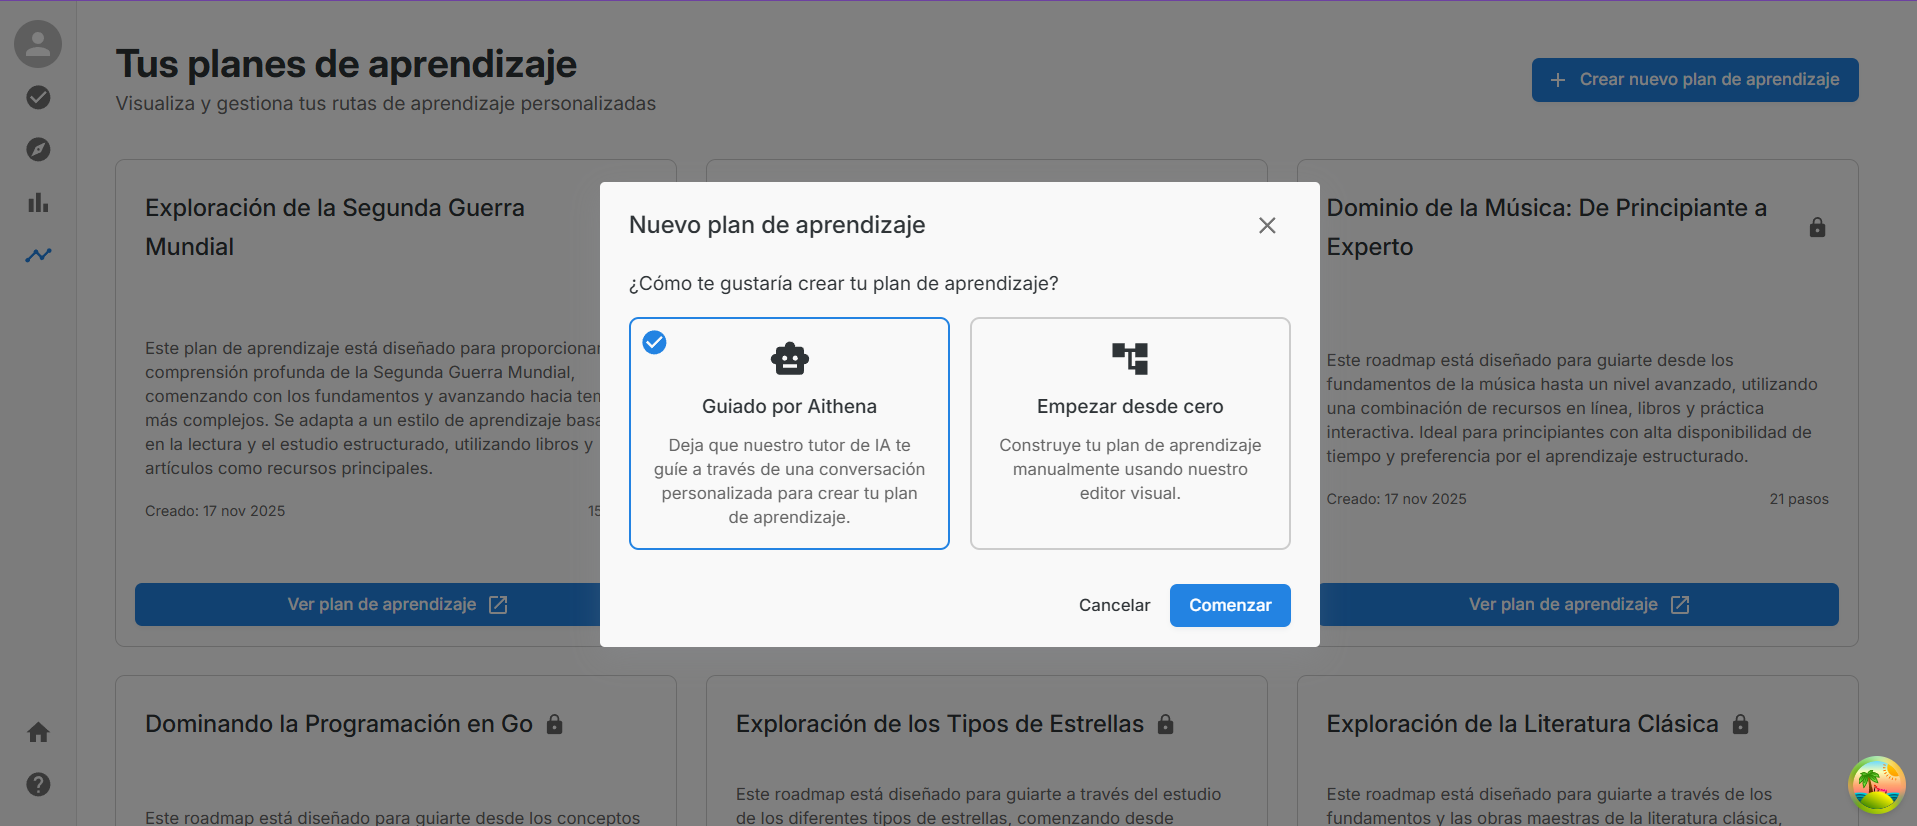
\includegraphics[width=0.95\textwidth]{Figuras/interfaces_AaA/creacion_roadmap.png}
\caption{Interfaz para la creación de roadmaps personalizados.}
\label{fig:aprender-creacion-roadmap}
\end{figure}

\noindent\textit{Descripción.} La interfaz permite elegir entre generar un roadmap automático mediante un agente de inteligencia artificial, que propone una ruta de aprendizaje personalizada, o bien construir un roadmap manual desde cero a través del editor visual.
\\
\\

% -------------------------------------------------
\subsection*{Edición mediante un editor visual de planes de aprendizaje}
% -------------------------------------------------

\noindent\textit{Descripción.} El editor permite añadir objetivos, crear tareas, reorganizar elementos mediante arrastrar y soltar, modificar descripciones y visualizar la relación jerárquica entre los componentes del roadmap. En las Figuras~\ref{fig:editor-inicial} a~\ref{fig:editor-estructura-general} se ilustran estas acciones dentro de la interfaz.

% (1) Editor vacío: lienzo y componentes
\begin{figure}[H]
\centering
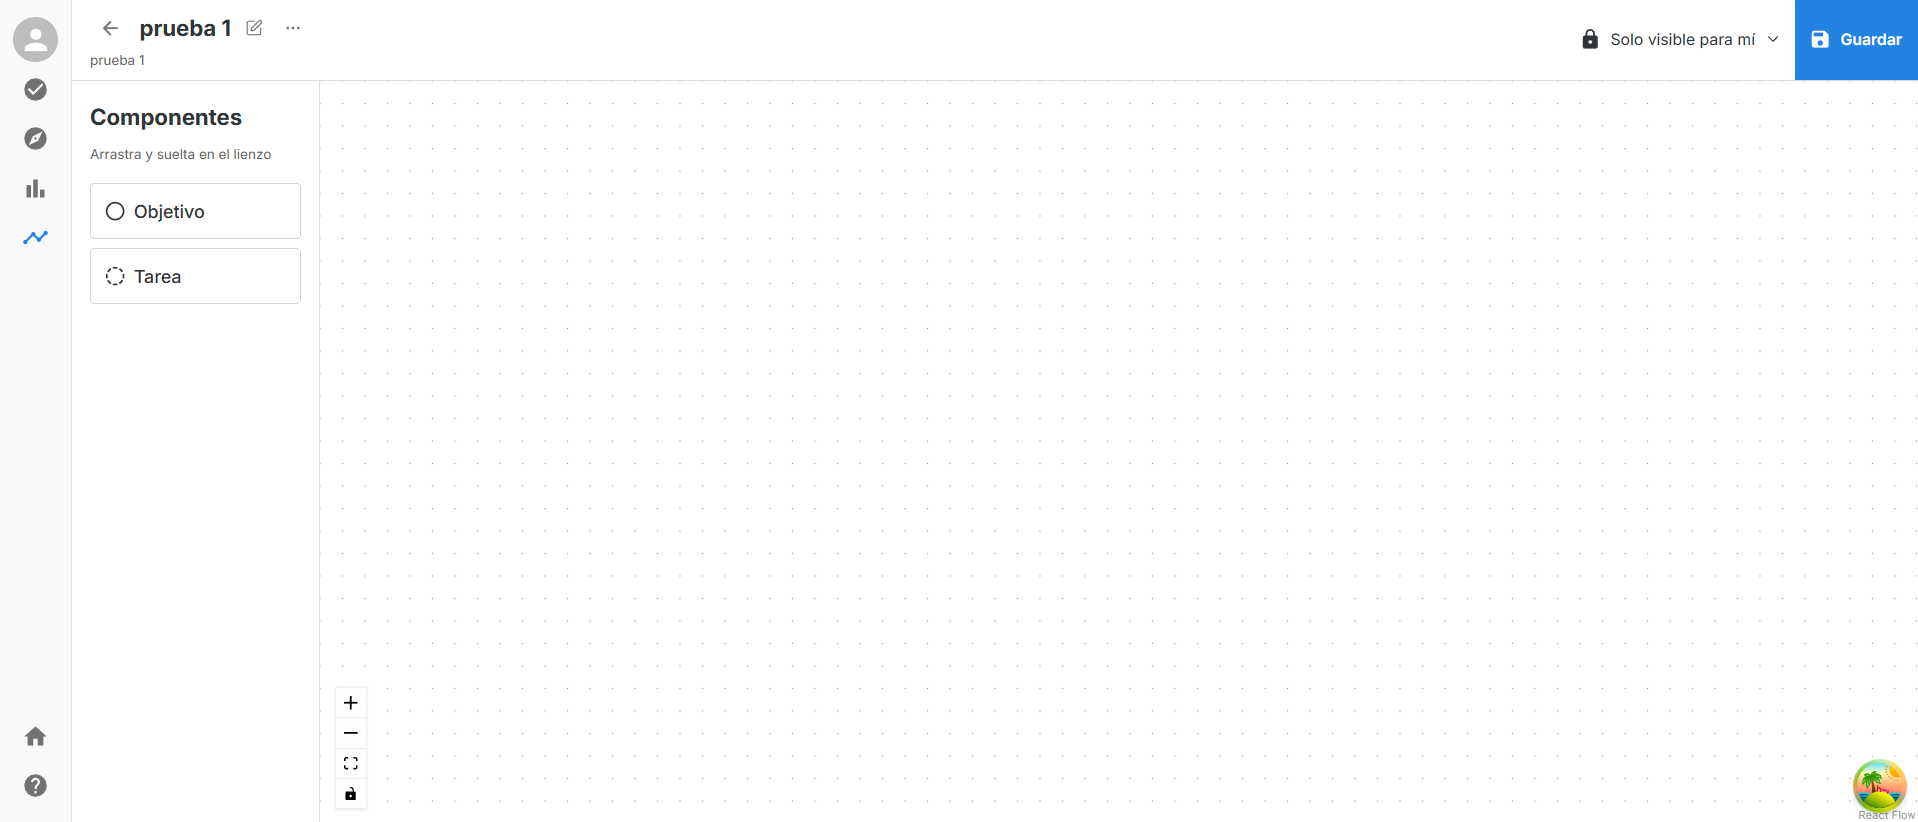
\includegraphics[width=0.95\textwidth]{Figuras/interfaces_AaA/editor_inicial.png}
\caption{Vista inicial del editor visual de planes de aprendizaje, con el lienzo y los componentes disponibles.}
\label{fig:editor-inicial}
\end{figure}

% (2) Arrastrar objetivo al lienzo
\begin{figure}[H]
\centering
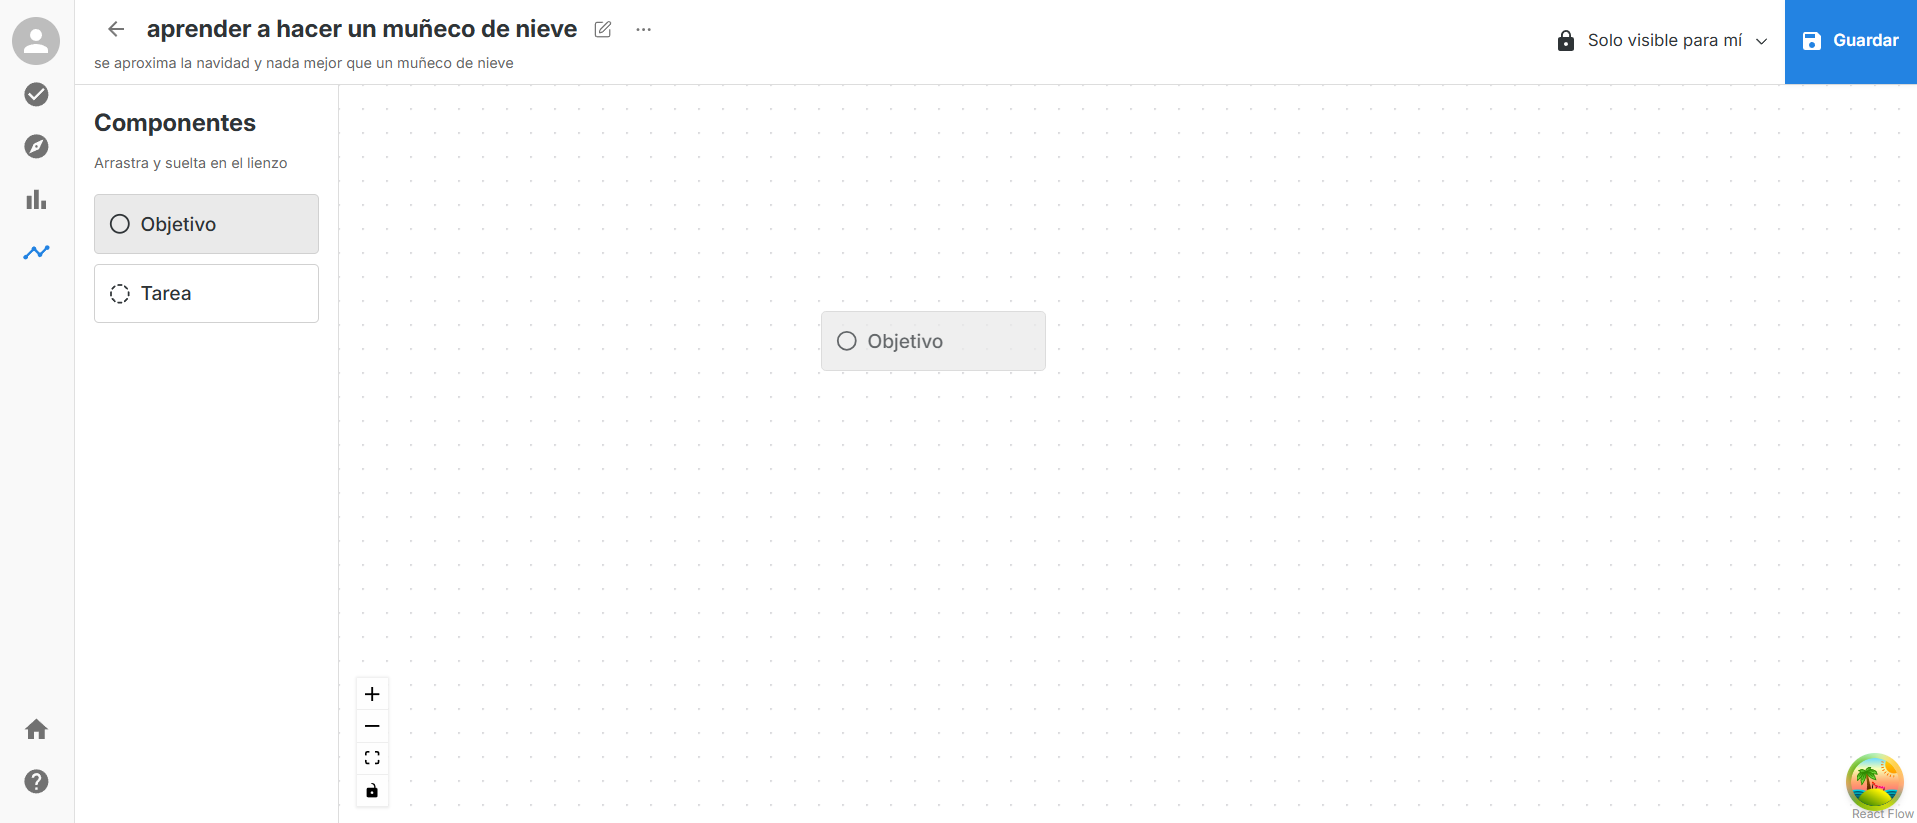
\includegraphics[width=0.95\textwidth]{Figuras/interfaces_AaA/editor_agregar_objetivo.png}
\caption{Agregar un nuevo objetivo arrastrándolo desde el panel de componentes hacia el lienzo.}
\label{fig:editor-agregar-objetivo}
\end{figure}

% (3) Arrastrar tarea al lienzo
\begin{figure}[H]
\centering
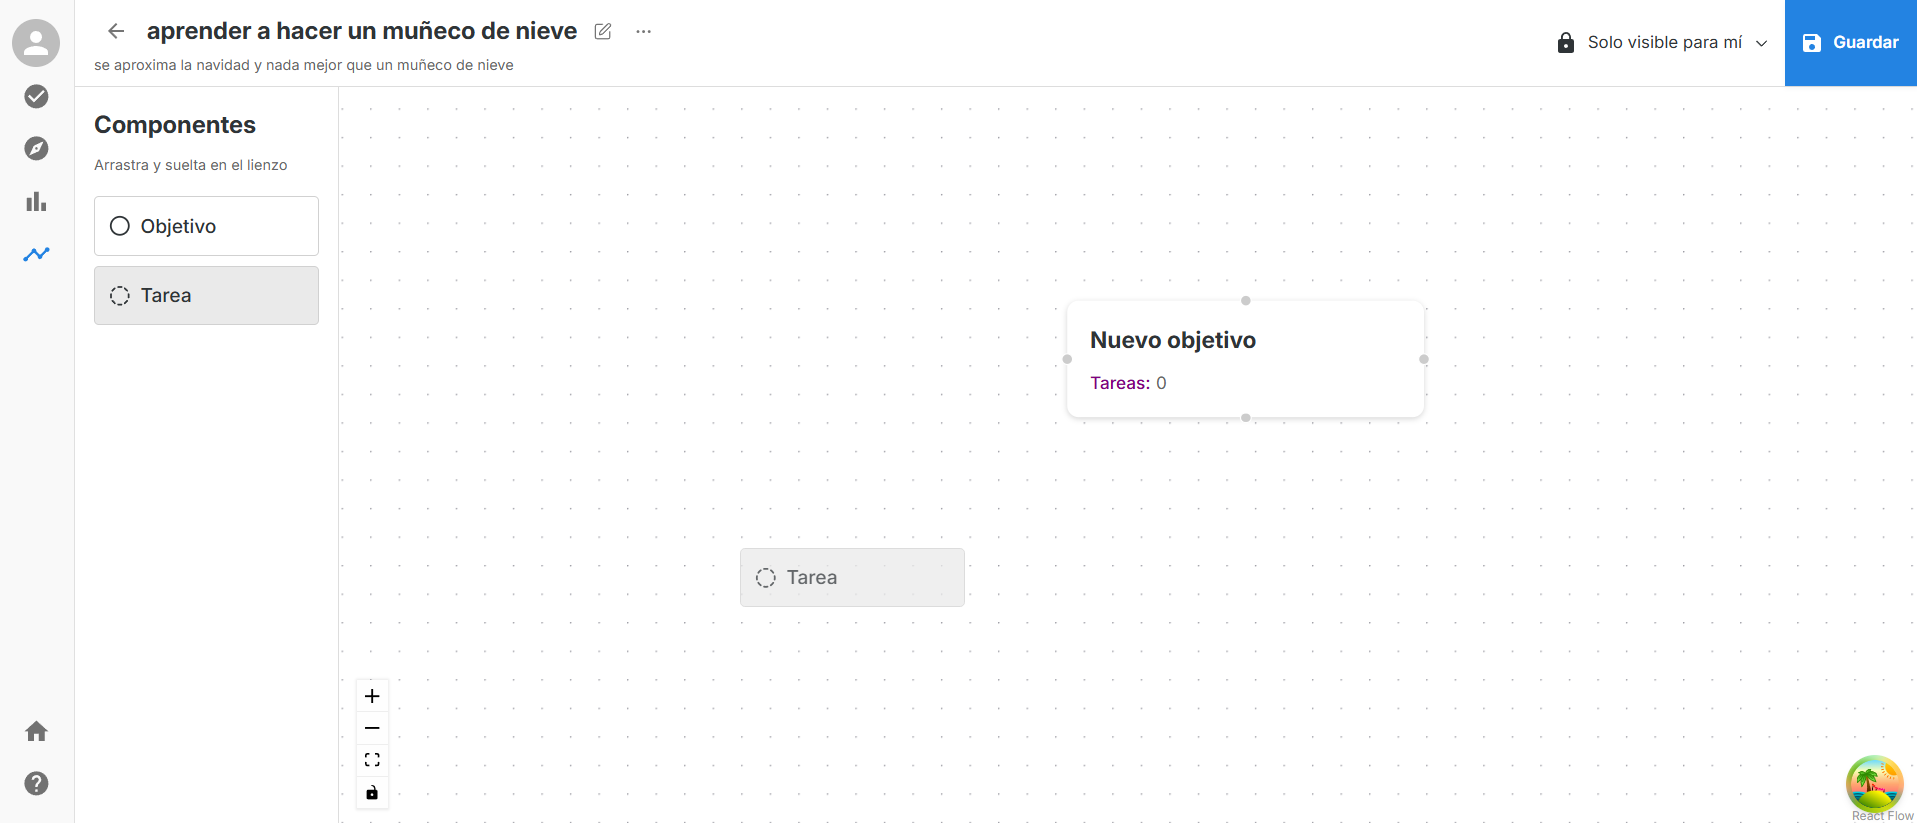
\includegraphics[width=0.95\textwidth]{Figuras/interfaces_AaA/editor_agregar_tarea.png}
\caption{Agregar una tarea al plan de aprendizaje mediante arrastrar y soltar.}
\label{fig:editor-agregar-tarea}
\end{figure}

% (4) Conectar tarea con objetivo
\begin{figure}[H]
\centering
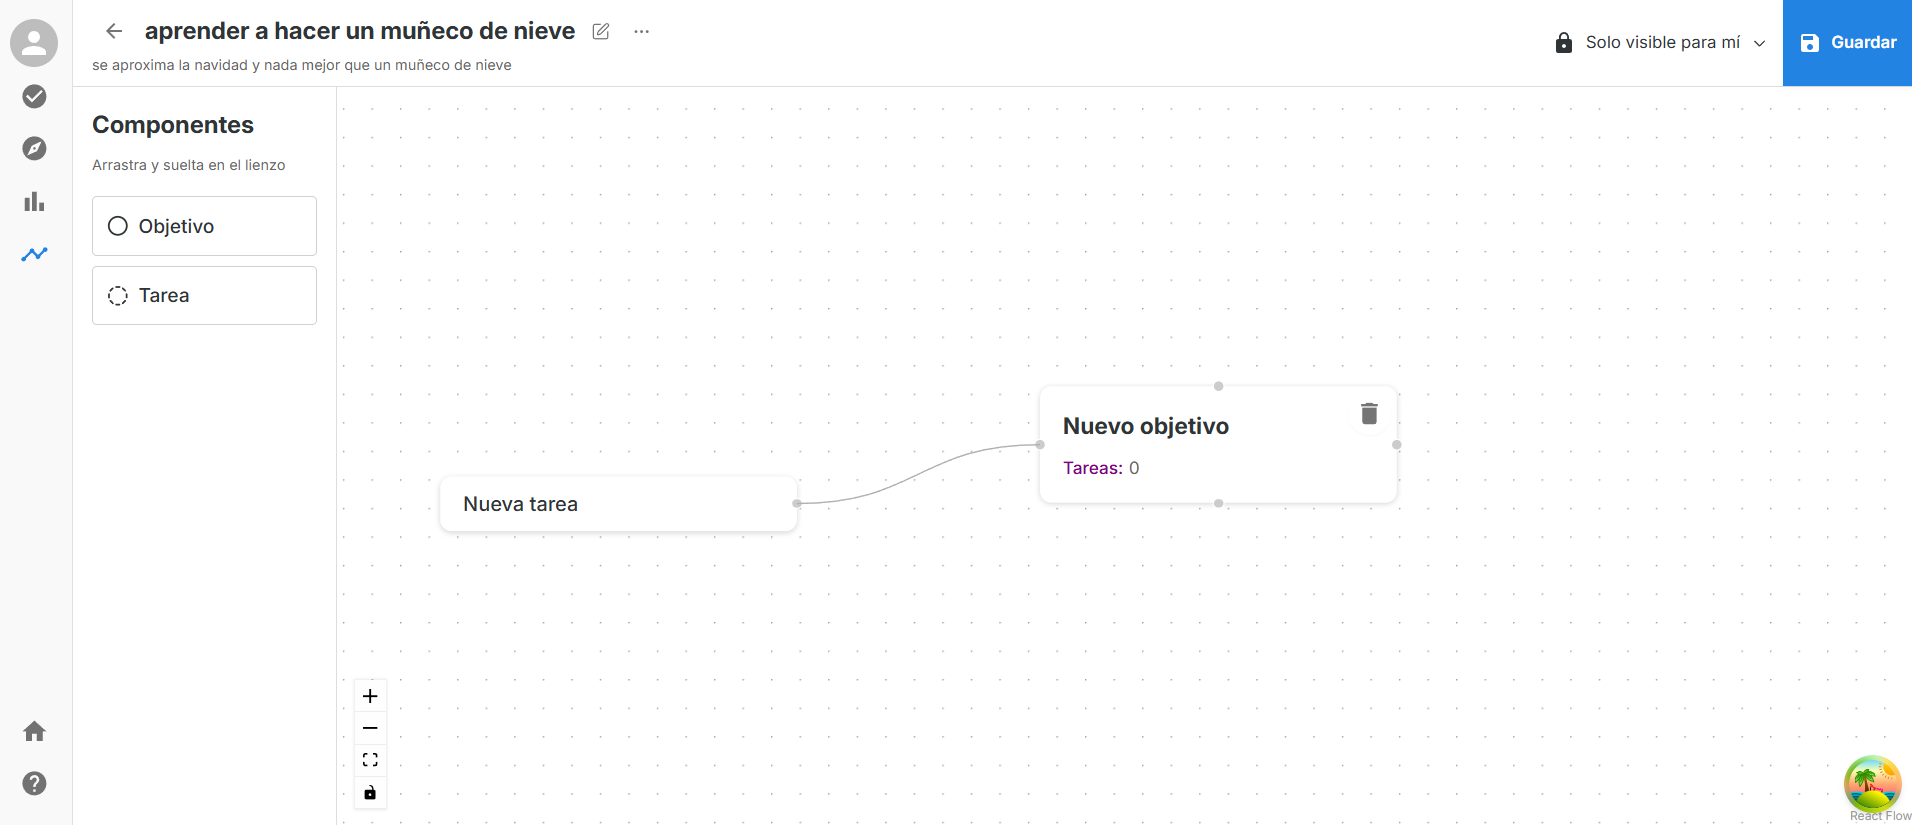
\includegraphics[width=0.95\textwidth]{Figuras/interfaces_AaA/editor_conectar_tarea_a_objetivo.png}
\caption{Conexión de una tarea con un objetivo, representando la relación entre ambos componentes.}
\label{fig:editor-conectar-tarea}
\end{figure}

% (5) Edición de contenido y enlaces del nodo
\begin{figure}[H]
\centering
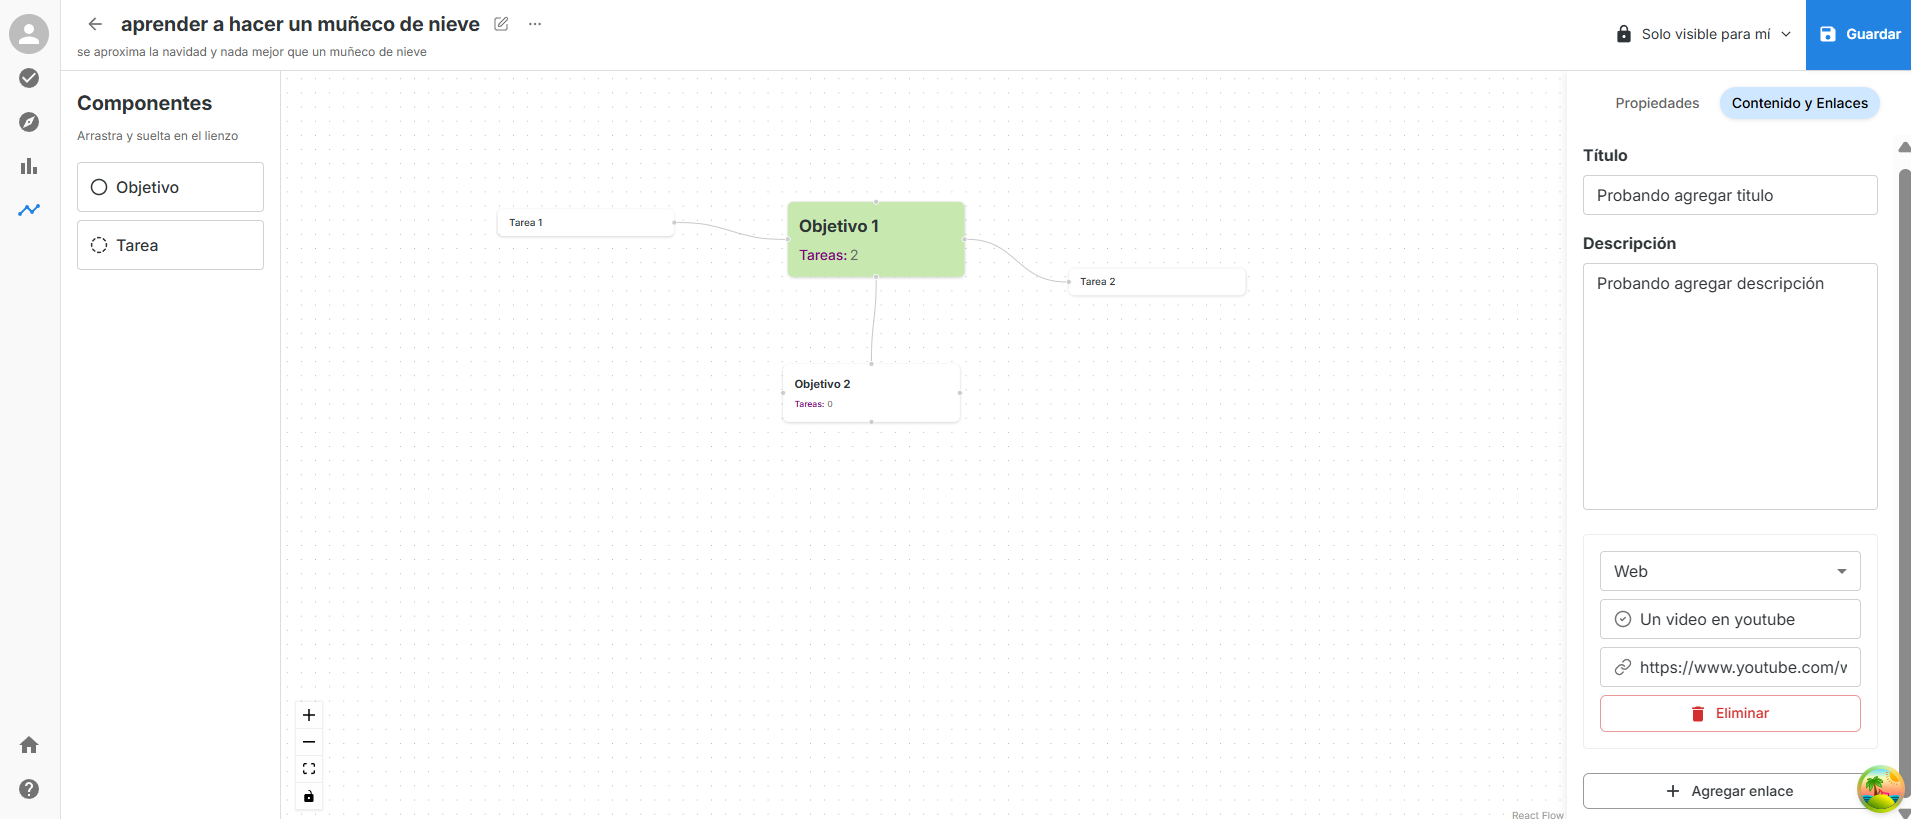
\includegraphics[width=0.95\textwidth]{Figuras/interfaces_AaA/editor_editar_contenido_y_enlaces.png}
\caption{Edición del contenido del objetivo y gestión de recursos asociados desde el panel lateral.}
\label{fig:editor-contenido-enlaces}
\end{figure}

% (6) Edición de propiedades visuales del nodo
\begin{figure}[H]
\centering
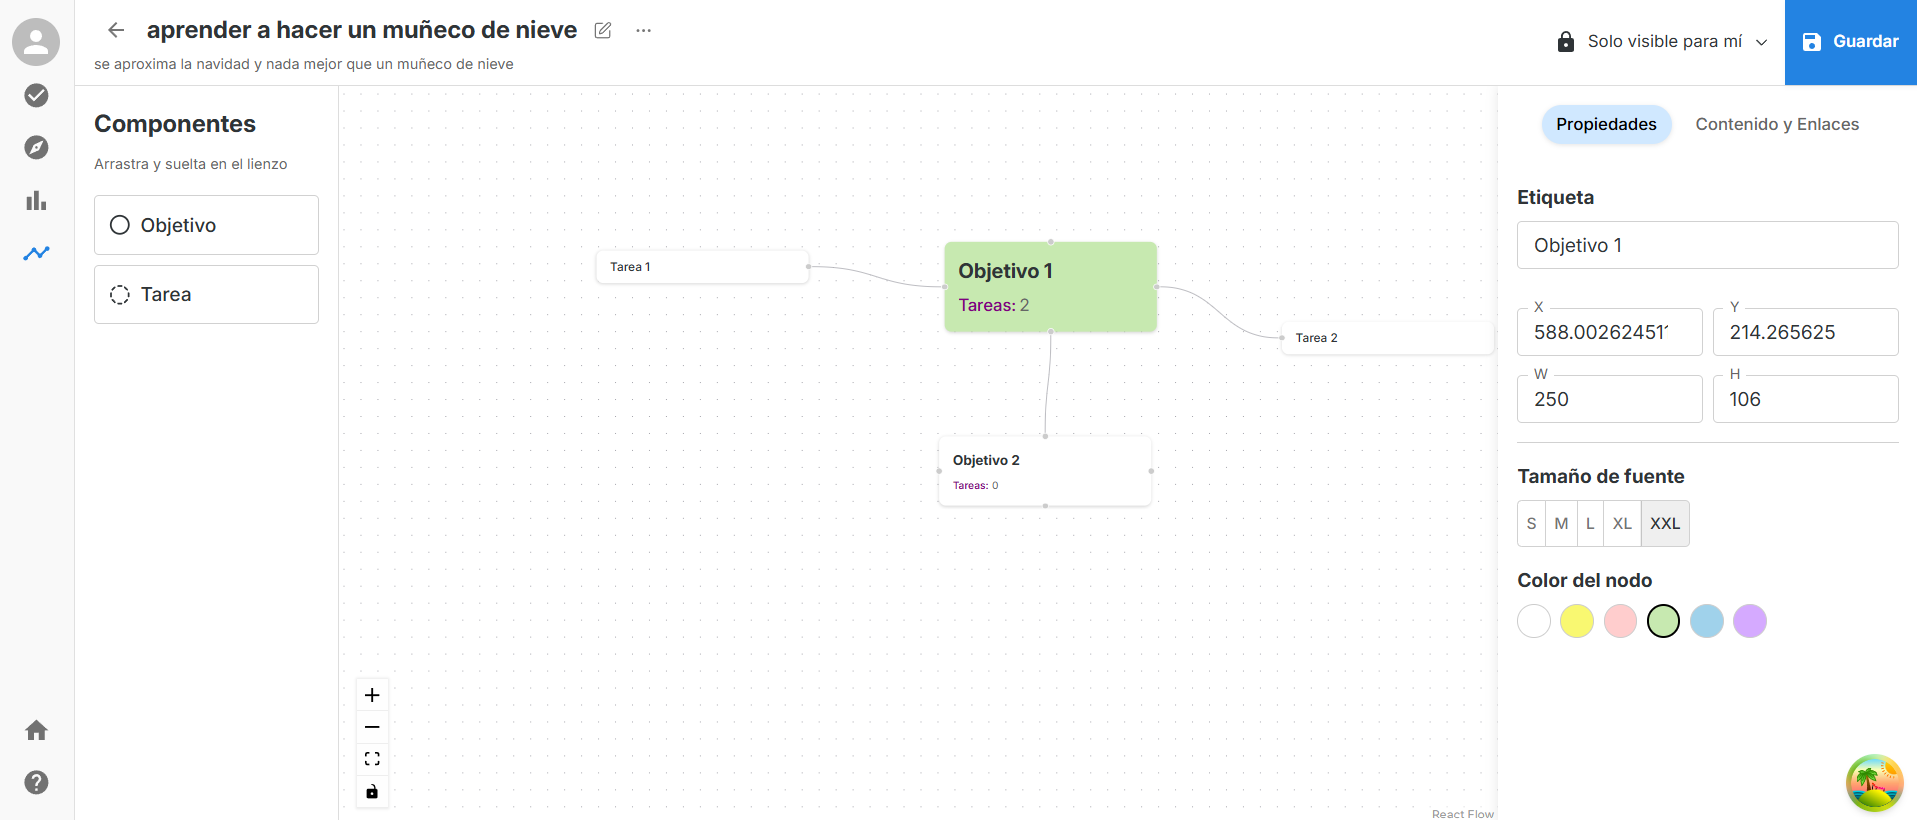
\includegraphics[width=0.95\textwidth]{Figuras/interfaces_AaA/editor_editar_propiedades_nodo.png}
\caption{Configuración de las propiedades visuales del objetivo (posición, tamaño y color del nodo).}
\label{fig:editor-propiedades-nodo}
\end{figure}

% (7) Estructura general del roadmap
\begin{figure}[H]
\centering
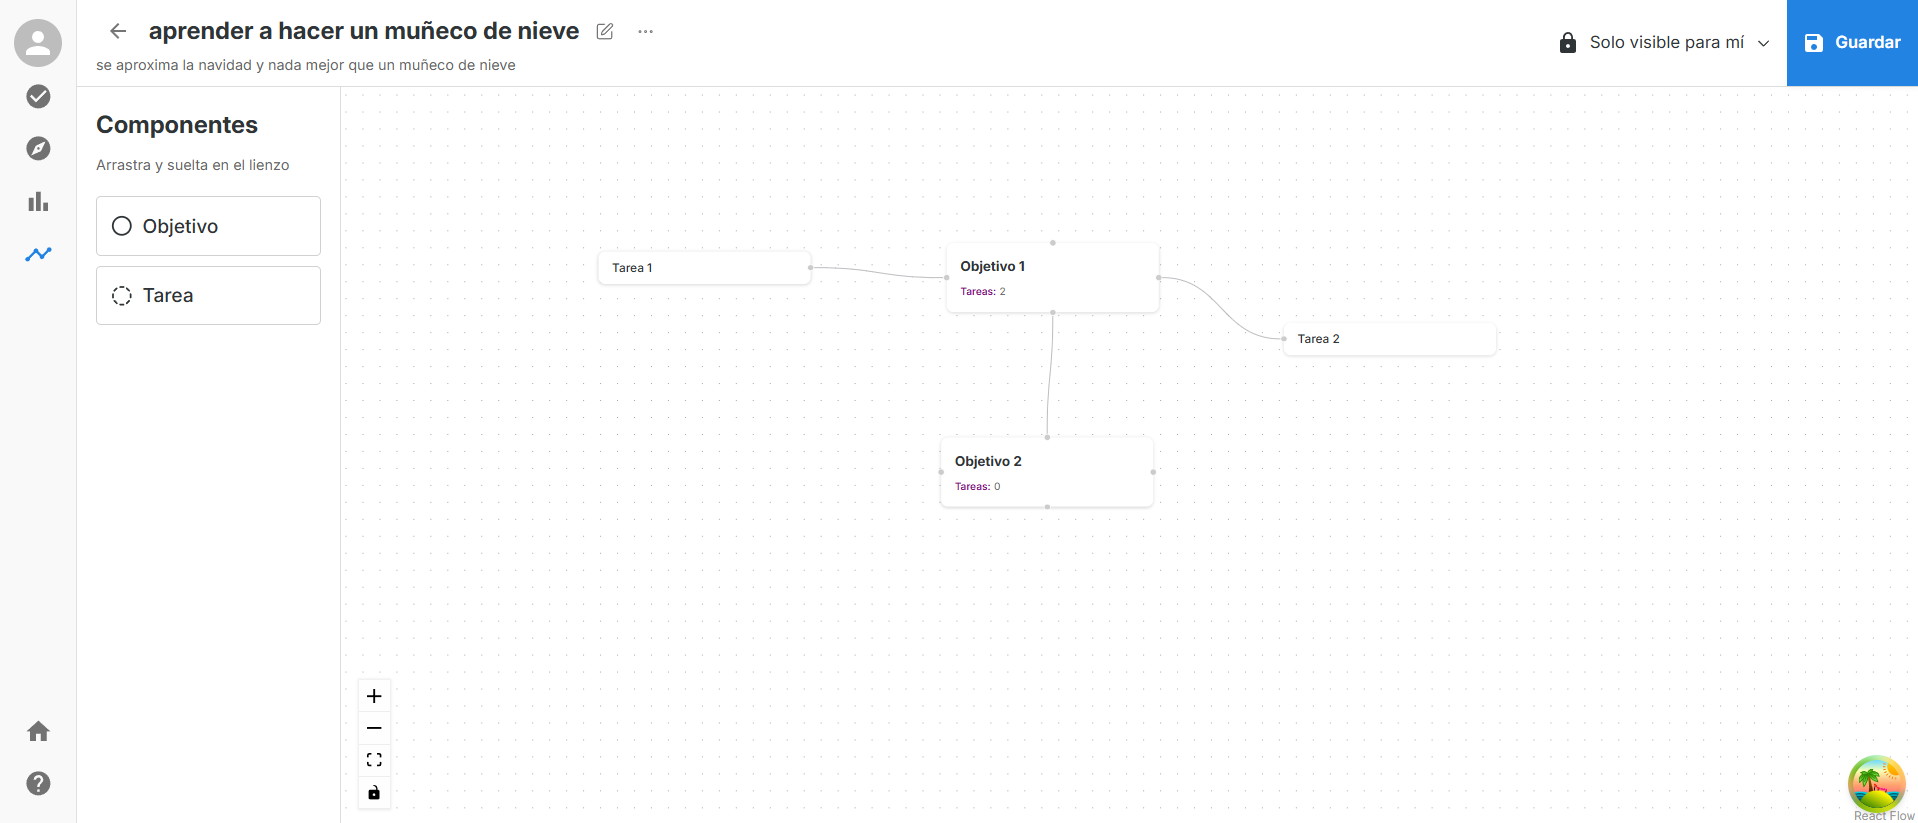
\includegraphics[width=0.95\textwidth]{Figuras/interfaces_AaA/editor_estructura_general.png}
\caption{Vista de la estructura general del roadmap, mostrando la relación jerárquica entre objetivos y tareas.}
\label{fig:editor-estructura-general}
\end{figure}

% -------------------------------------------------
\subsection*{Conversión entre roadmap y plan accionable}
% -------------------------------------------------

% (1) Opción: Crear plan accionable desde un roadmap
\begin{figure}[H]
\centering
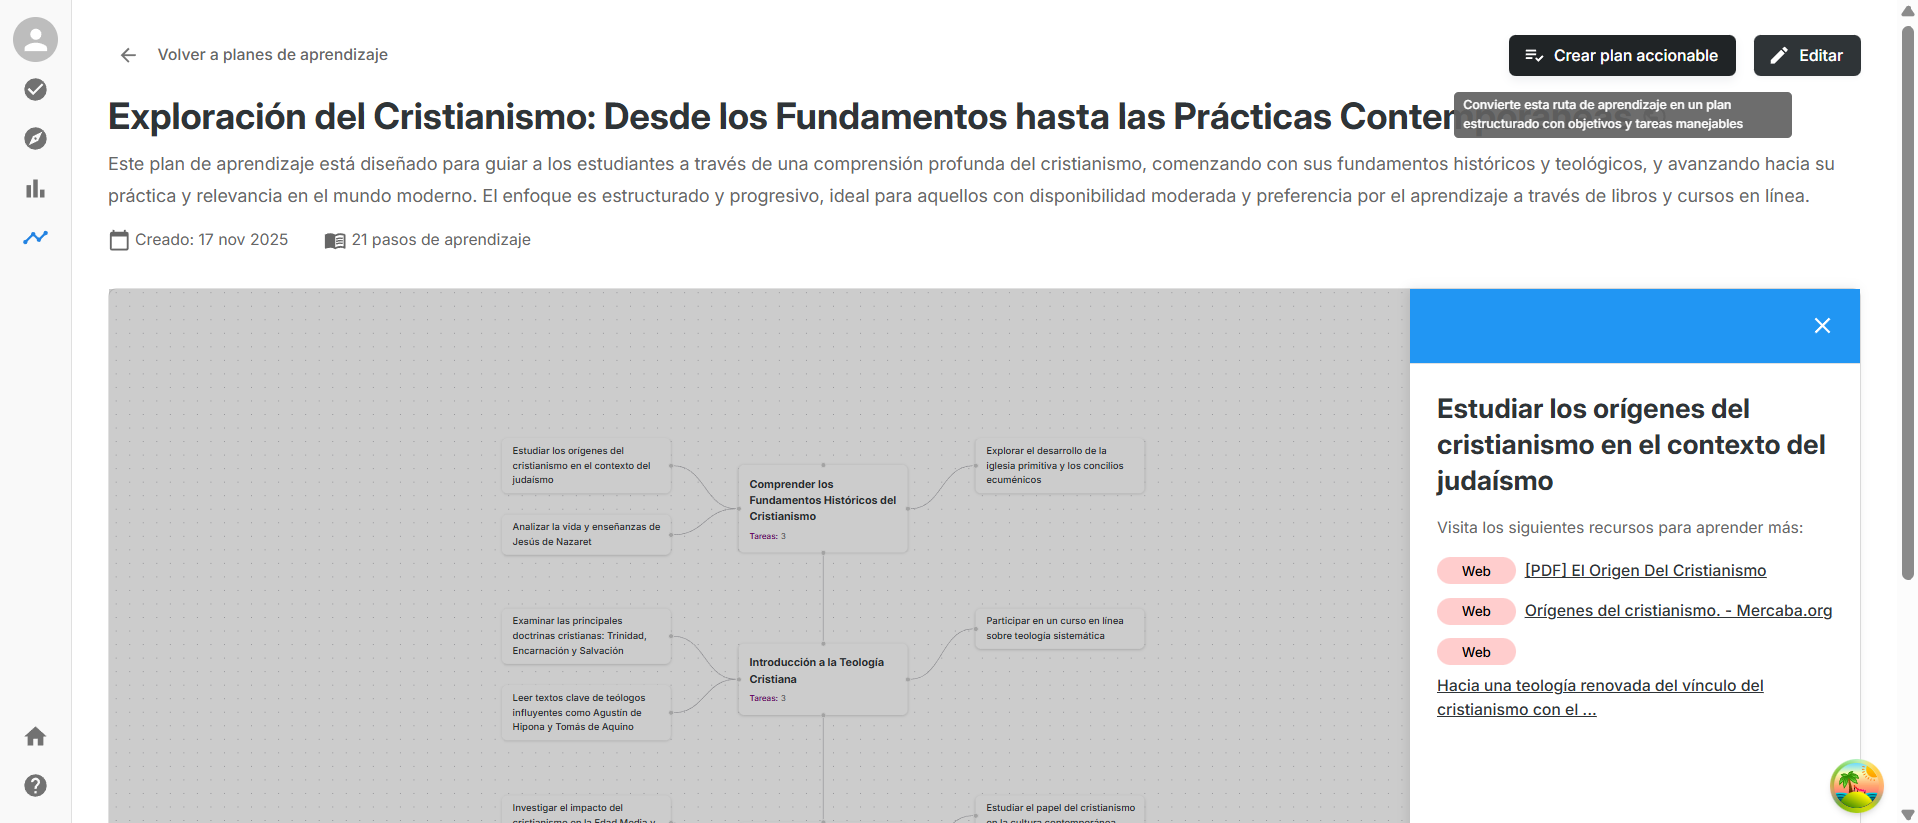
\includegraphics[width=0.95\textwidth]{Figuras/interfaces_AaA/roadmap_crear_plan_accionable.png}
\caption{Opción disponible en la vista del roadmap para crear un plan accionable a partir de la estructura diseñada.}
\label{fig:crear-plan-accionable}
\end{figure}

\noindent\textit{Descripción.} Desde la vista del roadmap, el estudiante puede convertir la ruta de aprendizaje en un plan accionable con un solo clic. Esta función genera automáticamente la meta principal, los objetivos y las tareas basadas en el contenido del roadmap, manteniendo su organización jerárquica.

% (2) Transformar plan accionable a roadmap
\begin{figure}[H]
\centering
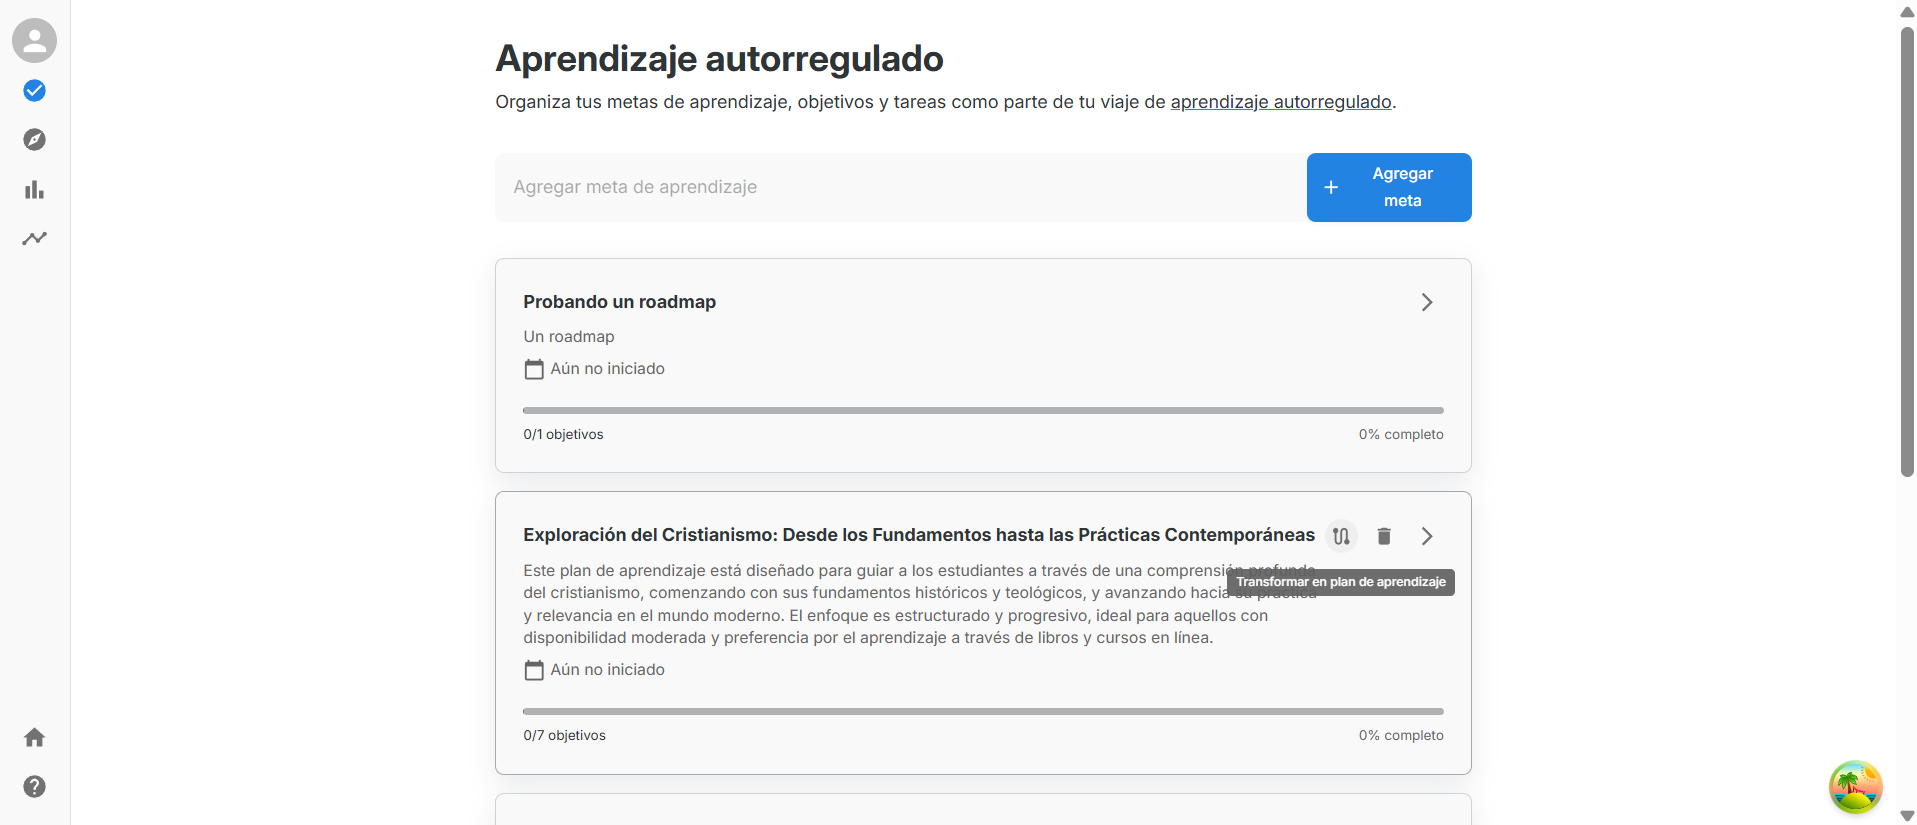
\includegraphics[width=0.95\textwidth]{Figuras/interfaces_AaA/plan_accionable_transformar_a_roadmap.png}
\caption{Interfaz que permite transformar un plan accionable existente nuevamente en un roadmap visual.}
\label{fig:accionable-a-roadmap}
\end{figure}

\noindent\textit{Descripción.} La conversión inversa permite visualizar un plan estructurado como un roadmap, facilitando la comprensión global de su organización y permitiendo reorganizar la estructura mediante el editor visual.


% (3) Lista de metas del plan accionable
\begin{figure}[H]
\centering
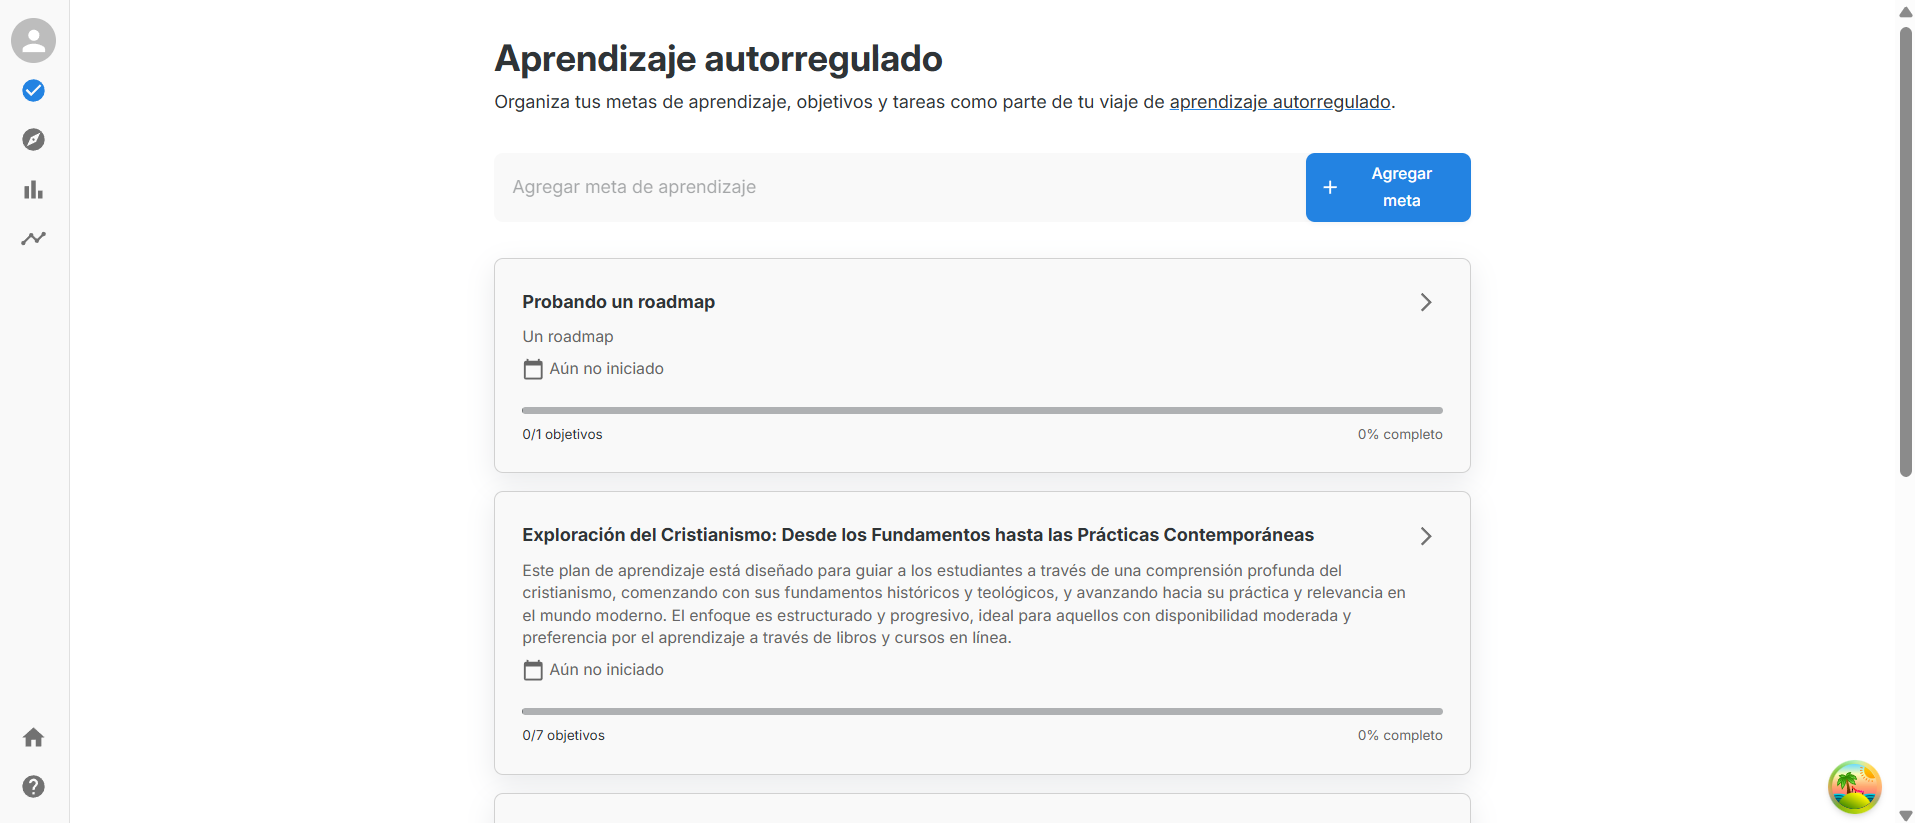
\includegraphics[width=0.95\textwidth]{Figuras/interfaces_AaA/plan_accionable_lista_metas.png}
\caption{Vista general del módulo de aprendizaje autorregulado, mostrando las metas generadas a partir del roadmap.}
\label{fig:accionable-lista-metas}
\end{figure}

\noindent\textit{Descripción.} Una vez generado el plan accionable, este aparece en la vista general del módulo, donde el estudiante puede acceder a su progreso, ver la cantidad de objetivos asociados y gestionar el avance en cada uno de ellos.

% (4) Detalle de una meta convertida
\begin{figure}[H]
\centering
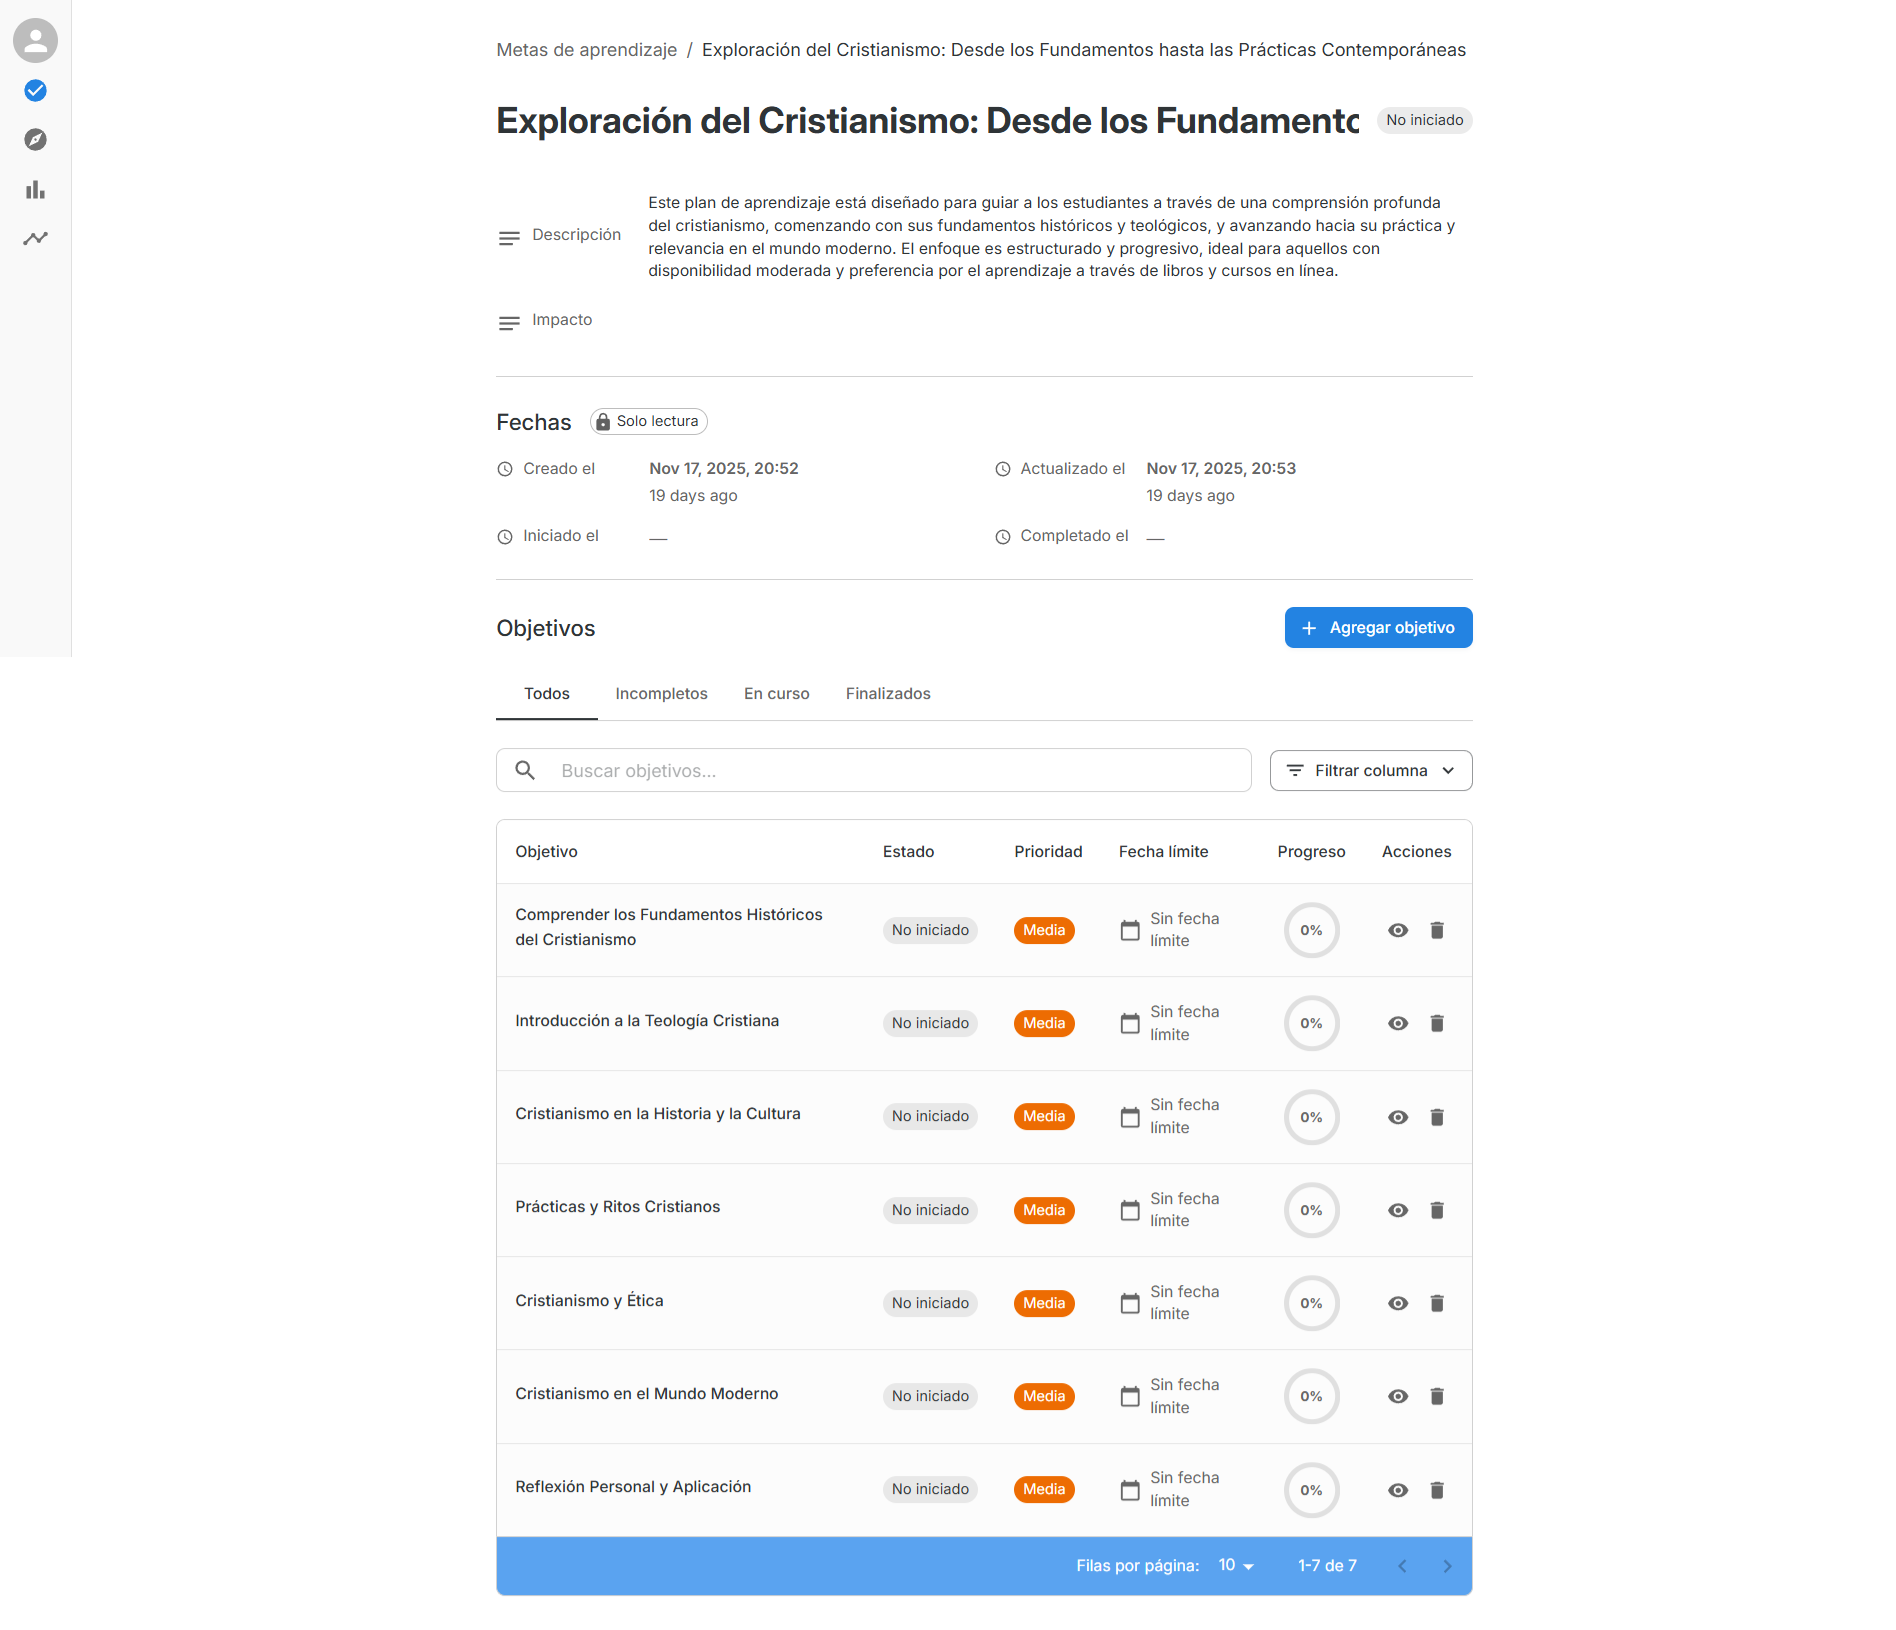
\includegraphics[width=0.95\textwidth]{Figuras/interfaces_AaA/plan_accionable_detalle_meta.png}
\caption{Vista detallada de la meta generada desde el roadmap, mostrando la lista completa de objetivos asociados.}
\label{fig:accionable-detalle-meta}
\end{figure}

\noindent\textit{Descripción.} La meta incluye todos los objetivos derivados del roadmap. Al convertirse en un plan accionable, cada objetivo se inicializa con una prioridad media y un estado por defecto, permitiendo al estudiante navegar entre ellos y revisar su contenido dentro de la estructura operativa del plan.


% (5) Detalle de un objetivo dentro del plan accionable
\begin{figure}[H]
\centering
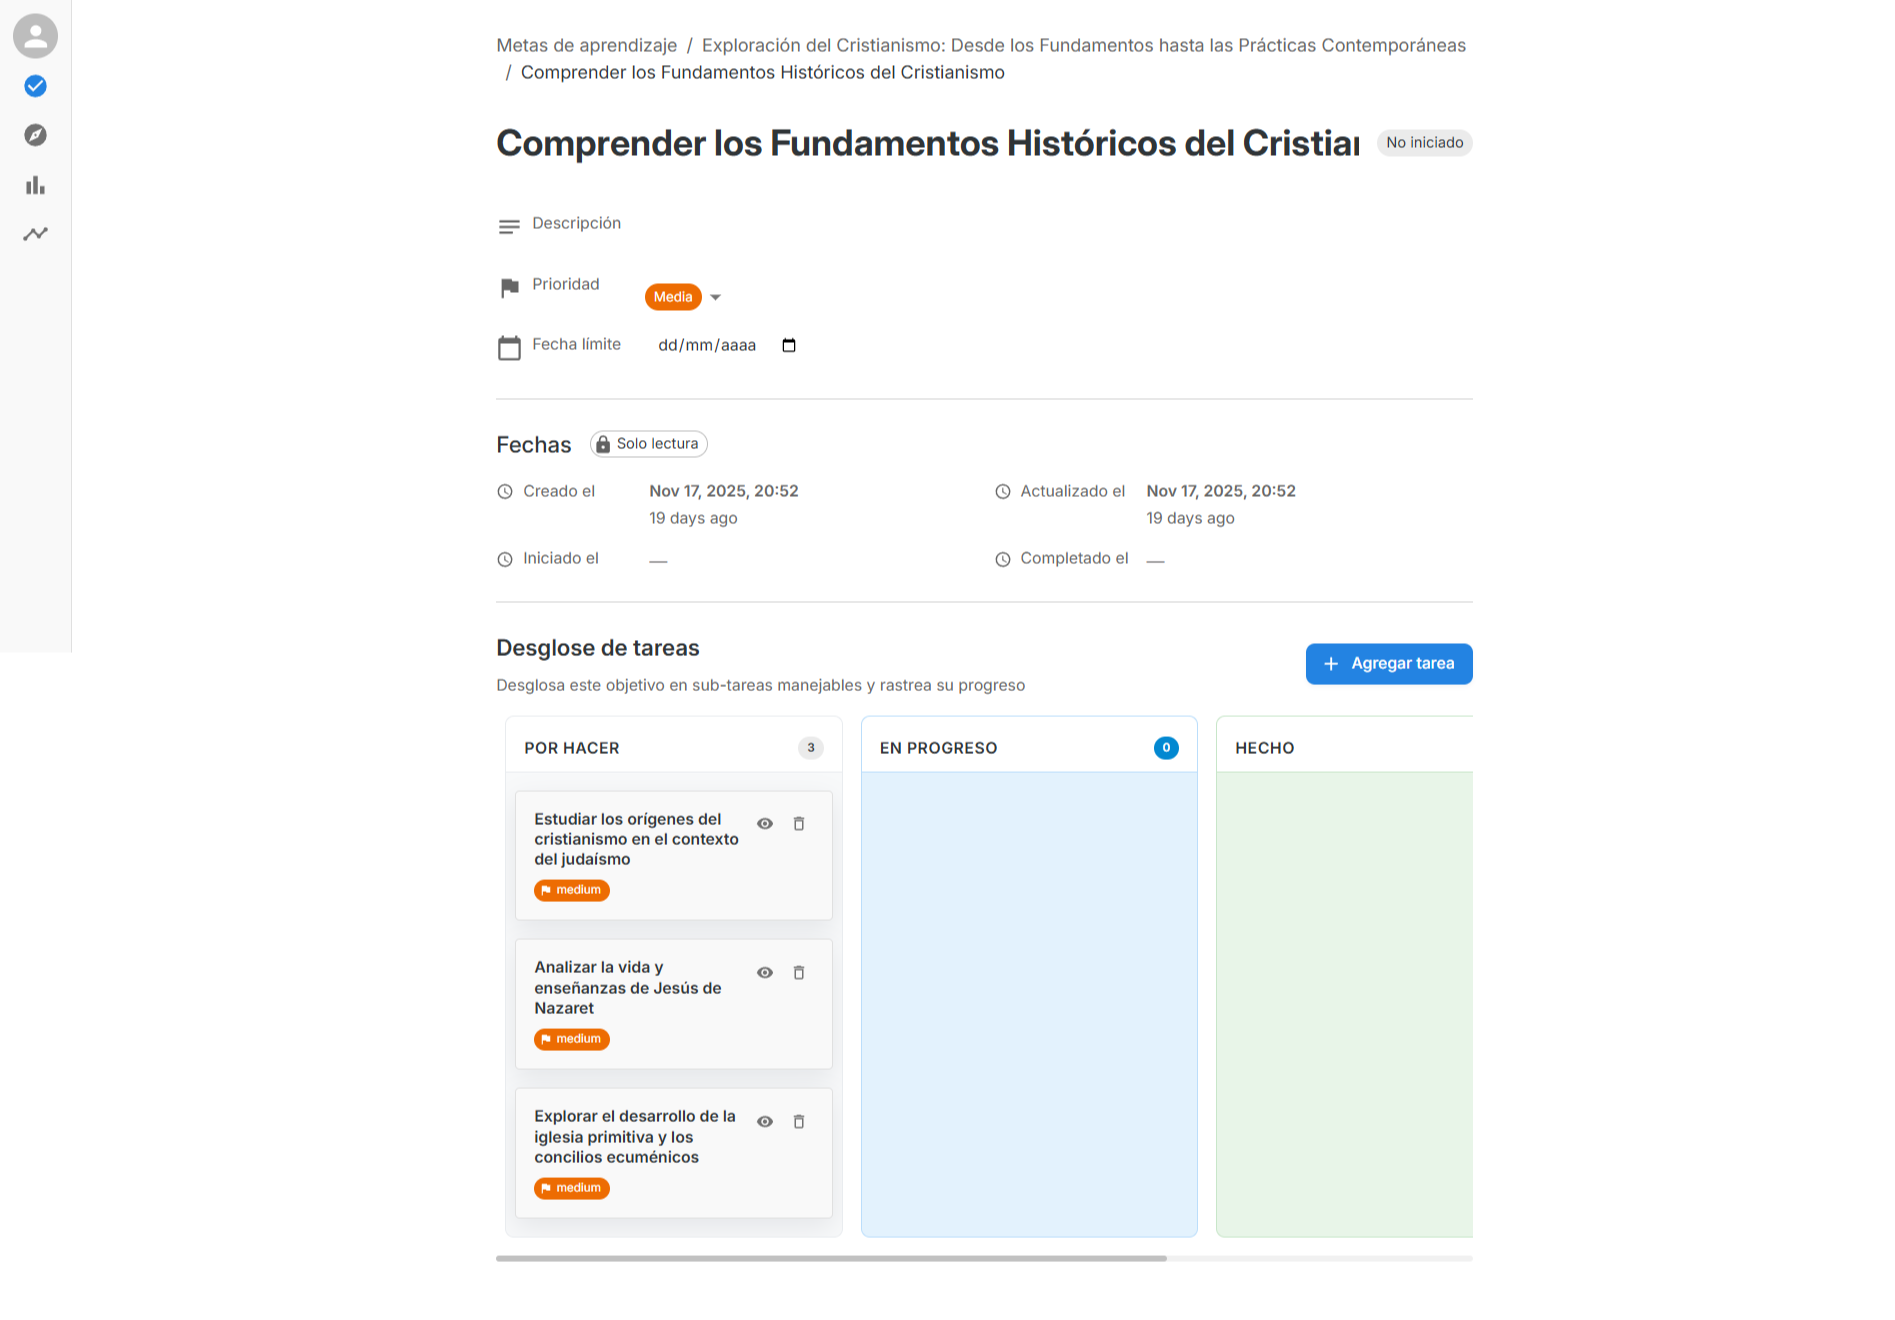
\includegraphics[width=0.95\textwidth]{Figuras/interfaces_AaA/plan_accionable_detalle_objetivo.png}
\caption{Interfaz de detalle de un objetivo dentro del plan accionable, con su desglose de tareas organizado por columnas de progreso.}
\label{fig:accionable-detalle-objetivo}
\end{figure}

\noindent\textit{Descripción.} Las tareas derivadas del roadmap se organizan automáticamente dentro del objetivo correspondiente y se presentan en columnas de \textit{Por hacer}, \textit{En progreso} y \textit{Hecho}. Al convertirse en plan accionable, cada tarea se inicializa con una prioridad media por defecto, manteniendo el título y la estructura definidos en el roadmap.



% (6) Detalle de una tarea convertida con recursos transferidos
\begin{figure}[H]
\centering
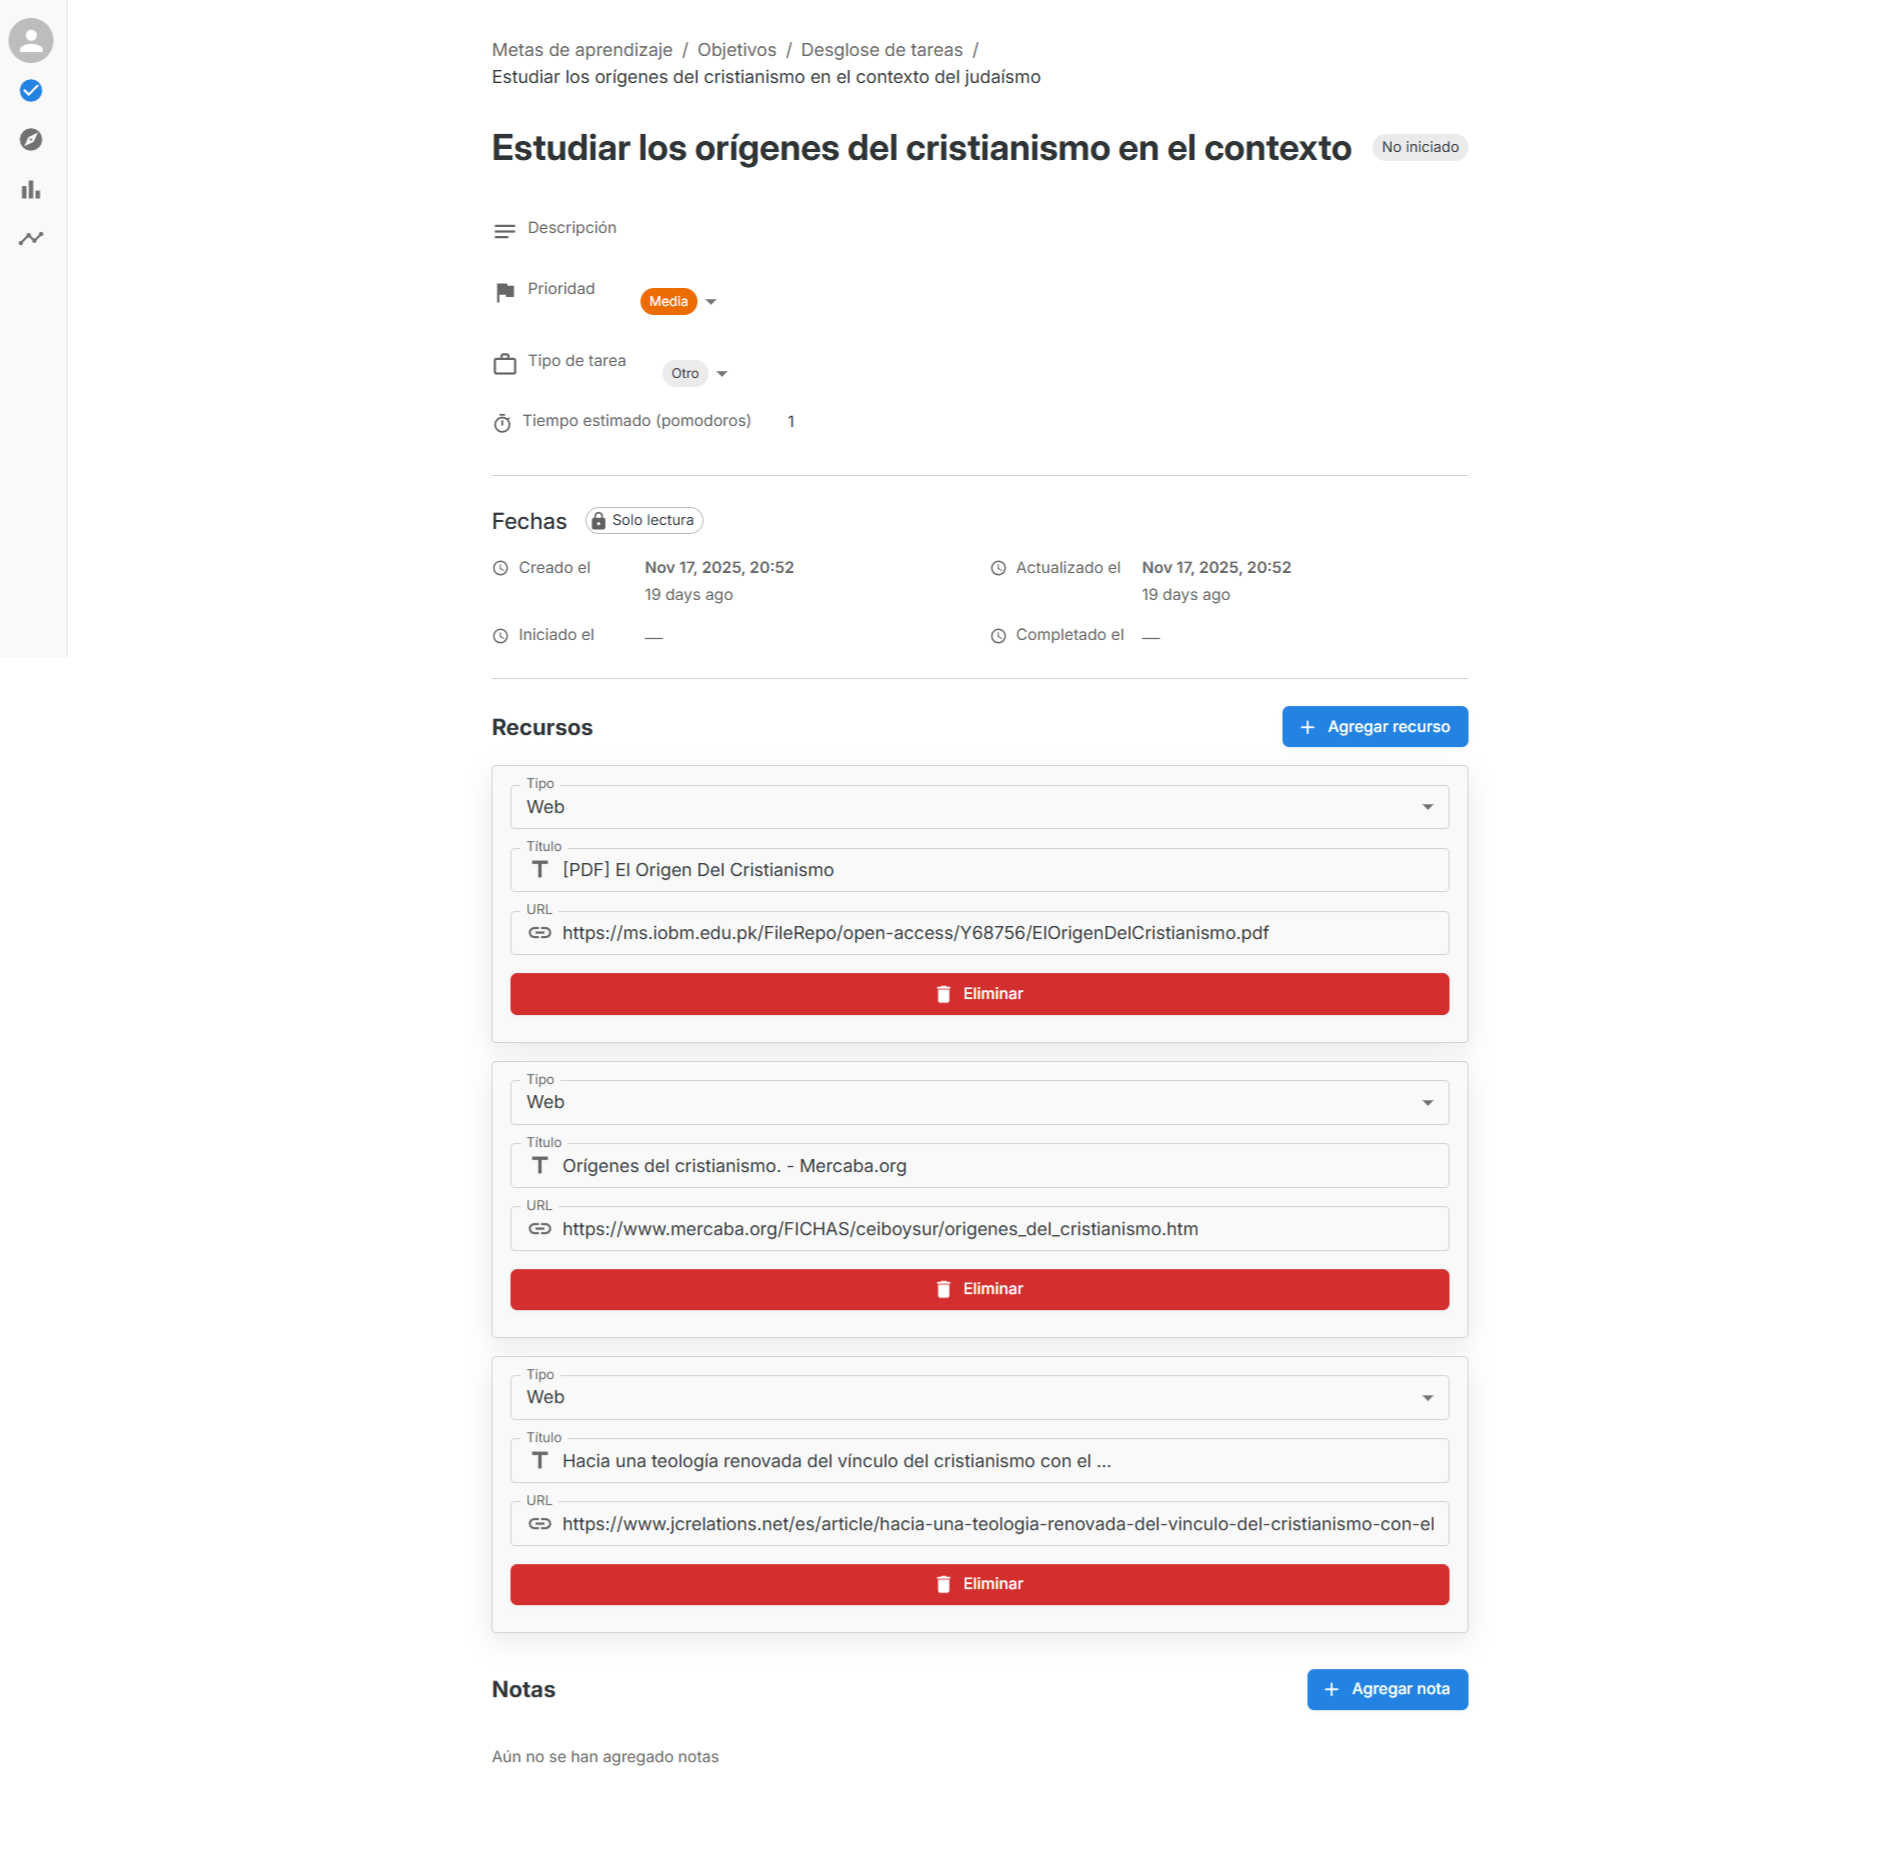
\includegraphics[width=0.95\textwidth]{Figuras/interfaces_AaA/plan_accionable_detalle_tarea.png}
\caption{Detalle de una tarea del plan accionable, incluyendo los recursos transferidos automáticamente desde el roadmap.}
\label{fig:accionable-detalle-tarea}
\end{figure}

\noindent\textit{Descripción.} Cuando una tarea en el roadmap incluye recursos (enlaces, documentos, videos, artículos), estos se trasladan automáticamente a la tarea equivalente del plan accionable. Esta transferencia garantiza consistencia entre la fase de planificación visual y la fase de ejecución del aprendizaje.

% -------------------------------------------------
% Exploración de planes de aprendizaje públicos
% -------------------------------------------------
\subsection*{Exploración de planes de aprendizaje públicos}

\begin{figure}[H]
\centering
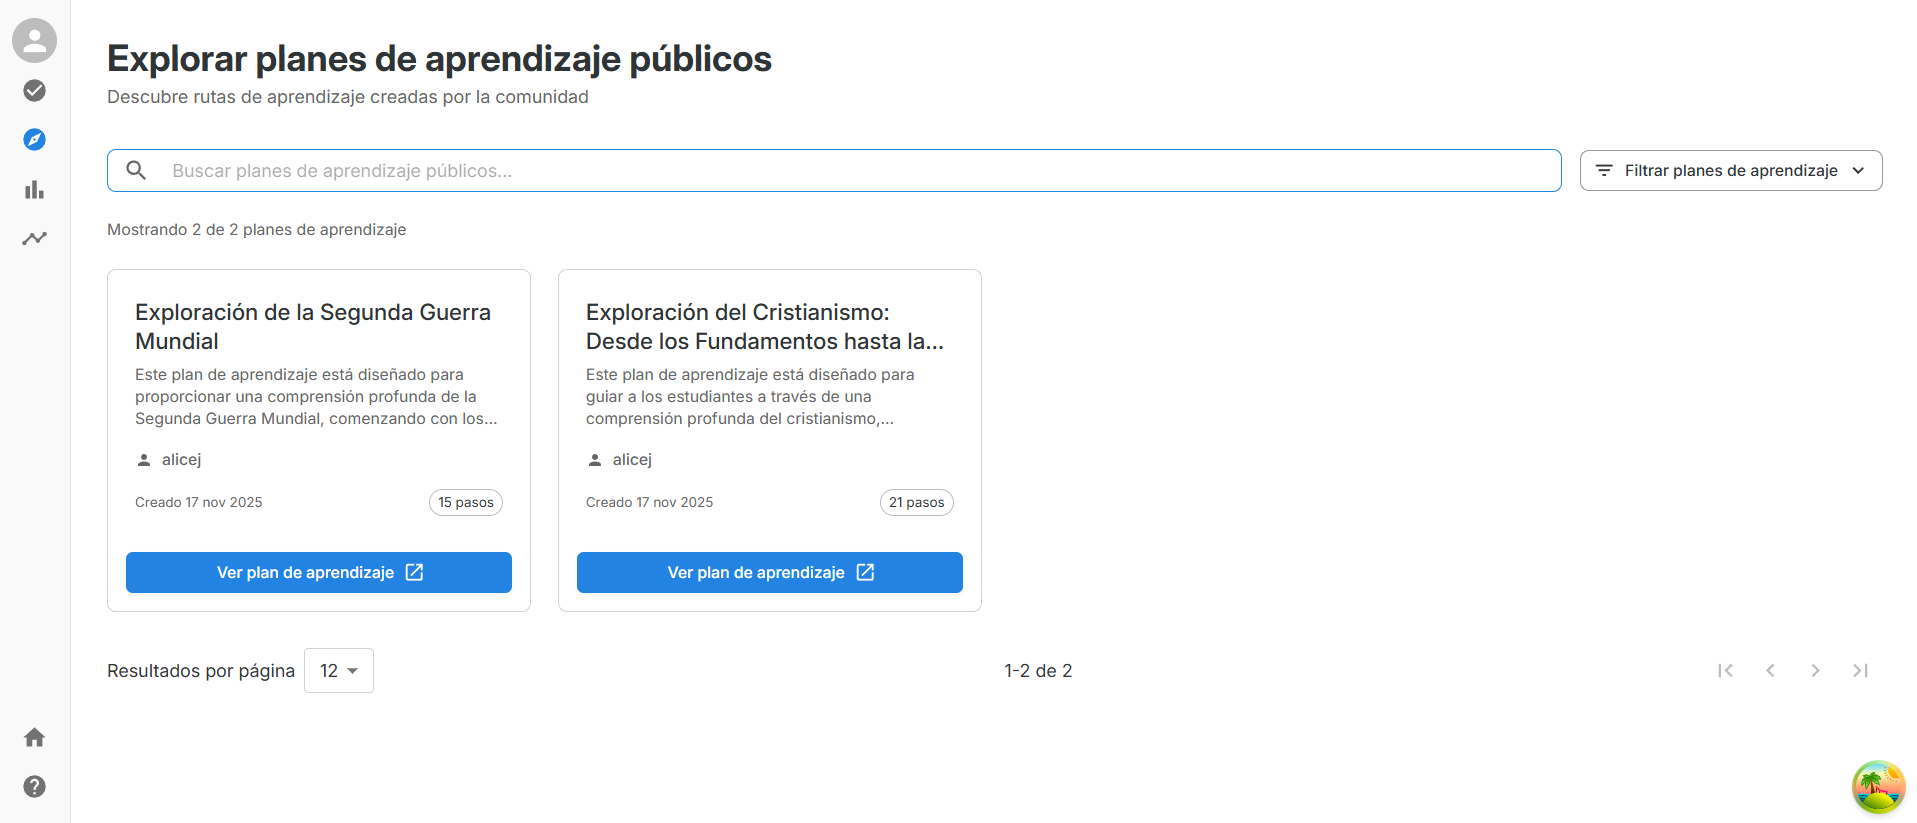
\includegraphics[width=0.95\textwidth]{Figuras/interfaces_AaA/exploracion_planes_publicos.png}
\caption{Listado de planes de aprendizaje públicos disponibles para exploración.}
\label{fig:exploracion-planes-publicos}
\end{figure}

\noindent\textit{Descripción.} La vista inicial muestra los planes públicos creados por la comunidad, junto con información relevante como título, autor, fecha de creación y número total de pasos del plan. Cada tarjeta permite acceder a la versión completa del plan para revisarlo antes de decidir su reutilización.

\begin{figure}[H]
\centering
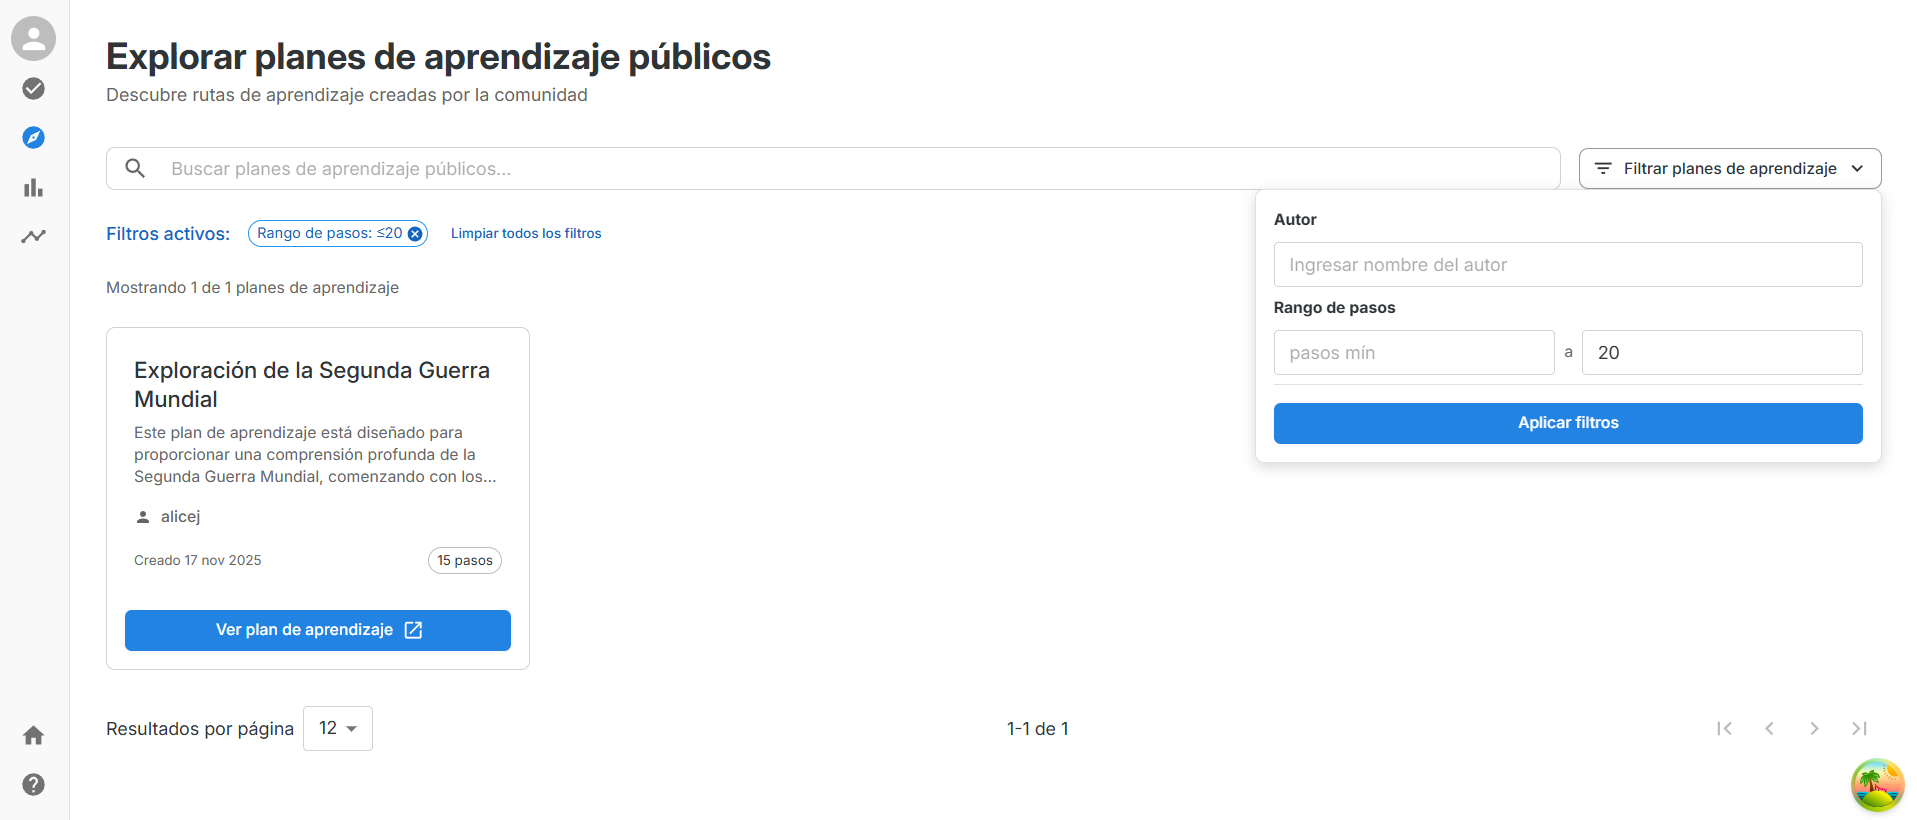
\includegraphics[width=0.95\textwidth]{Figuras/interfaces_AaA/exploracion_planes_publicos_filtros.png}
\caption{Aplicación de filtros por autor y rango de pasos en la exploración de planes públicos.}
\label{fig:exploracion-planes-publicos-filtros}
\end{figure}

\noindent\textit{Descripción.} El panel de filtrado permite acotar los resultados según criterios como el nombre del autor o el rango de pasos del plan. La interfaz actualiza la lista de resultados en función de los filtros aplicados, facilitando la búsqueda de modelos de referencia alineados con las necesidades del estudiante.

\subsection*{Copia y reutilización de planes públicos}

\begin{figure}[H]
\centering
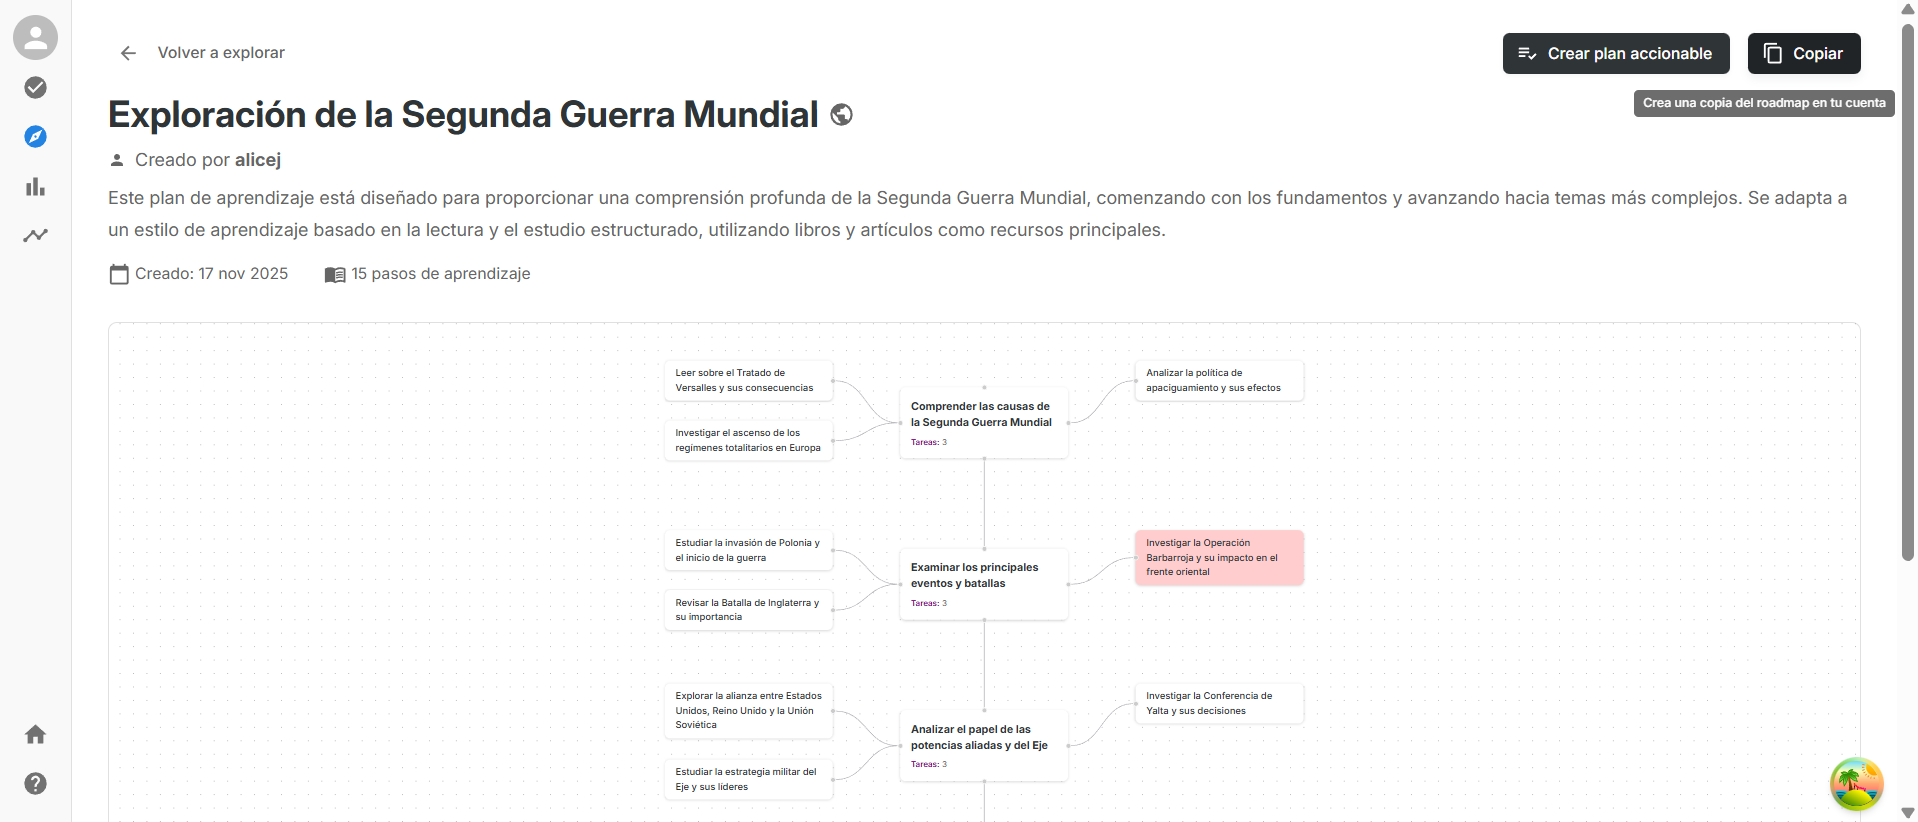
\includegraphics[width=0.95\textwidth]{Figuras/interfaces_AaA/copia_reutilizacion_planes_publicos.png}
\caption{Opción para copiar un plan de aprendizaje público hacia la cuenta del estudiante.}
\label{fig:copiar-plan-publico}
\end{figure}

\noindent\textit{Descripción.} El sistema permite que el estudiante tome cualquier plan de aprendizaje público y lo copie a su cuenta para reutilizarlo o adaptarlo a sus propias metas. Esta acción crea automáticamente una nueva versión del plan con \textbf{visibilidad privada}, asegurando que solo el estudiante pueda editarla o reorganizarla según sus necesidades.
\\
\\

\begin{figure}[H]
\centering
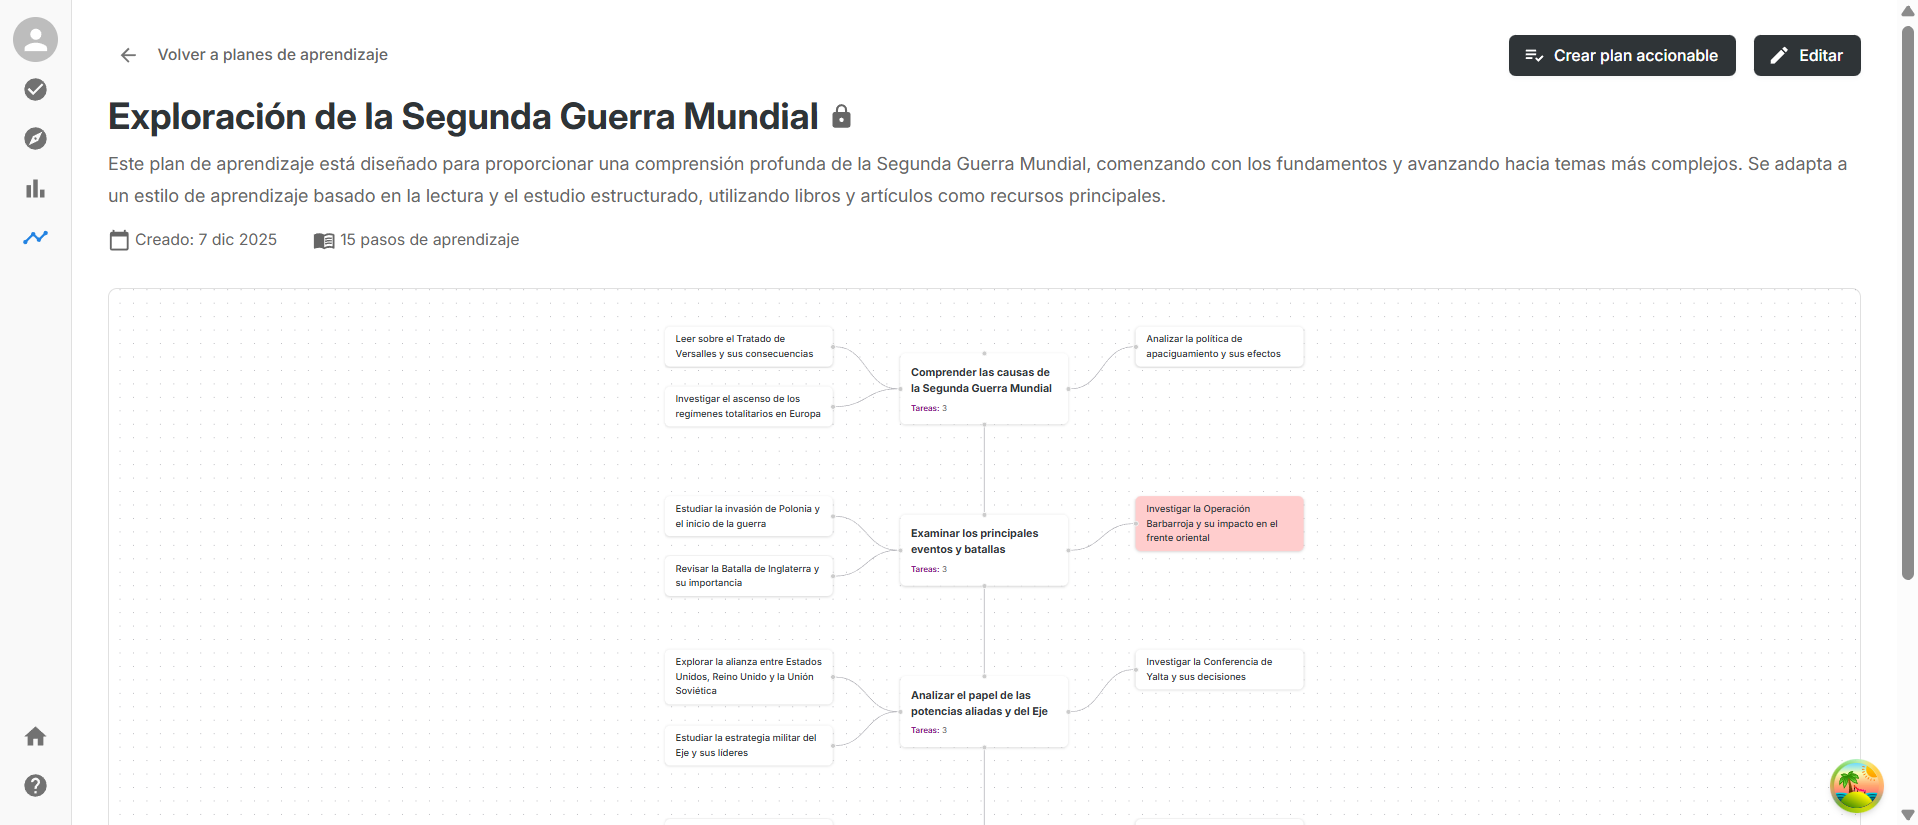
\includegraphics[width=0.95\textwidth]{Figuras/interfaces_AaA/plan_publico_copiado_en_cuenta.png}
\caption{Plan público copiado, ahora disponible como plan privado en la cuenta del estudiante.}
\label{fig:plan-publico-copiado}
\end{figure}

\noindent\textit{Descripción.} Una vez copiado, el plan aparece dentro del listado personal de metas de aprendizaje del estudiante, donde puede modificar objetivos, reorganizar tareas o transformar el plan en un roadmap visual si así lo requiere.

% -------------------------------------------------
\subsection*{Gestión de objetivos y tareas}
% -------------------------------------------------

\noindent Esta actividad se apoya en las mismas interfaces del editor visual y del plan accionable ya presentadas en las secciones anteriores, por lo que no se incluyen figuras adicionales.

% -------------------------------------------------
\subsection*{Seguimiento del progreso mediante Kanban}
% -------------------------------------------------
\noindent\textit{Descripción.} El tablero Kanban forma parte de la interfaz de detalle del objetivo dentro del plan accionable. En la Figura~\ref{fig:accionable-detalle-objetivo} se muestra cómo las tareas derivadas del roadmap se distribuyen automáticamente en columnas que reflejan su estado actual, facilitando el seguimiento del proceso de estudio.

% -------------------------------------------------
\subsection*{Desarrollo de tareas de aprendizaje}
% -------------------------------------------------
\noindent\textit{Descripción.} La Figura~\ref{fig:accionable-detalle-tarea} muestra la interfaz de detalle de una tarea dentro del plan accionable. Desde esta vista, el estudiante puede consultar los recursos transferidos automáticamente desde el roadmap, mientras que el cambio de estado de la tarea (iniciada, en pausa o completada) se realiza moviendo la tarjeta dentro del tablero Kanban.

% -------------------------------------------------
\subsection*{Agregación de recursos a las tareas}
% -------------------------------------------------

% (1) Formulario para agregar un recurso
\begin{figure}[H]
\centering
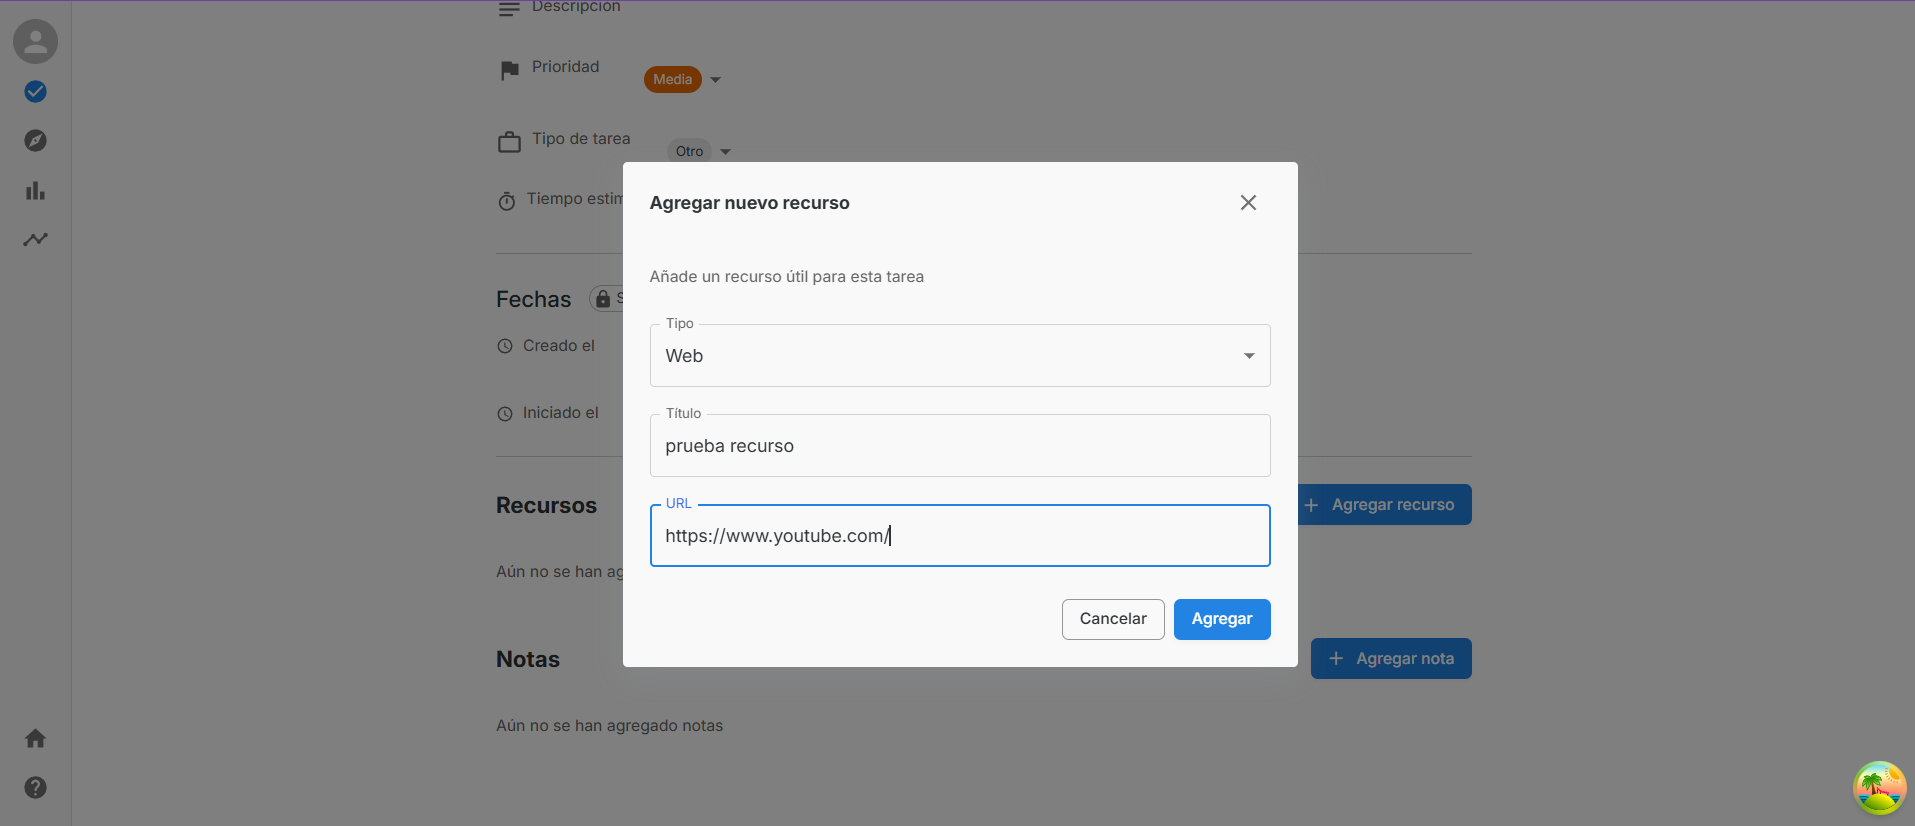
\includegraphics[width=0.95\textwidth]{Figuras/interfaces_AaA/agregar_recurso_tarea.png}
\caption{Formulario para agregar un nuevo recurso a una tarea dentro del plan accionable.}
\label{fig:agregar-recurso-tarea}
\end{figure}

\noindent\textit{Descripción.} Al seleccionar la opción \textit{Agregar recurso}, se despliega un formulario que permite especificar el tipo de recurso, su título y su URL. Al confirmar, el recurso queda asociado a la tarea.

% (2) Listado de recursos agregados
\begin{figure}[H]
\centering
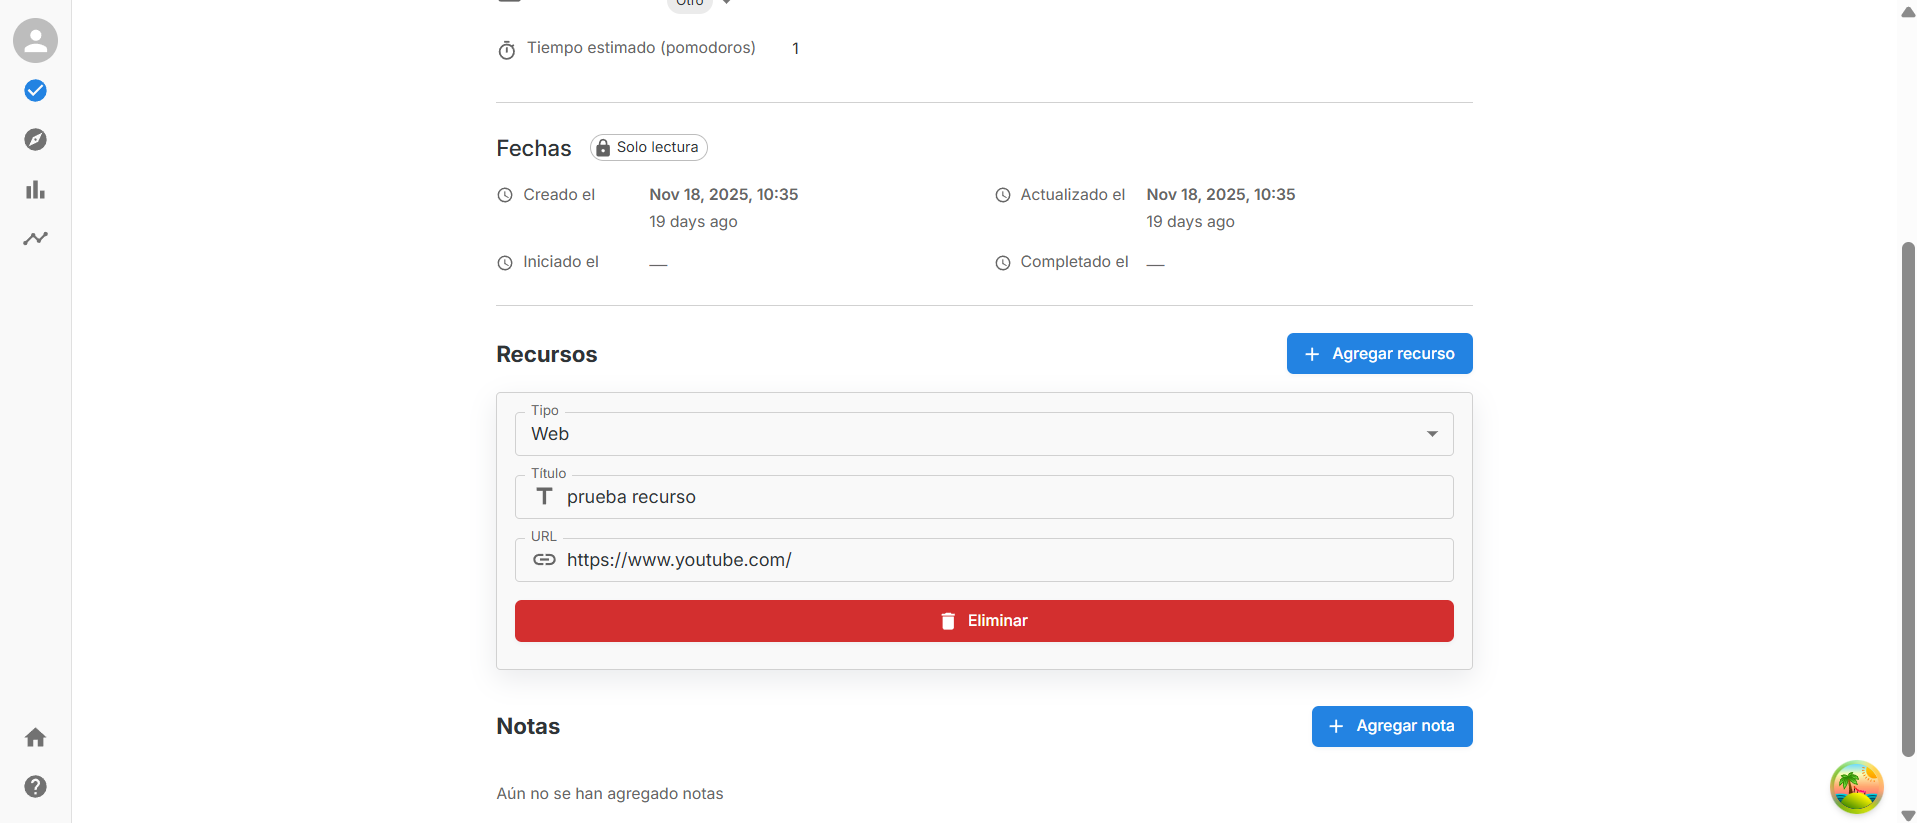
\includegraphics[width=0.95\textwidth]{Figuras/interfaces_AaA/tarea_recurso_listado.png}
\caption{Listado de recursos asociados a una tarea, con opciones para editarlos o eliminarlos.}
\label{fig:listado-recursos-tarea}
\end{figure}

\noindent\textit{Descripción.} Una vez agregado, el recurso aparece en el listado de la tarea, donde puede ser consultado, modificado o eliminado. Esta vista permite al estudiante gestionar de manera flexible los materiales que apoyan su proceso de aprendizaje.

% -------------------------------------------------
\subsection*{Registro de notas personales por tarea}
% -------------------------------------------------

% (1) Agregar nueva nota
\begin{figure}[H]
\centering
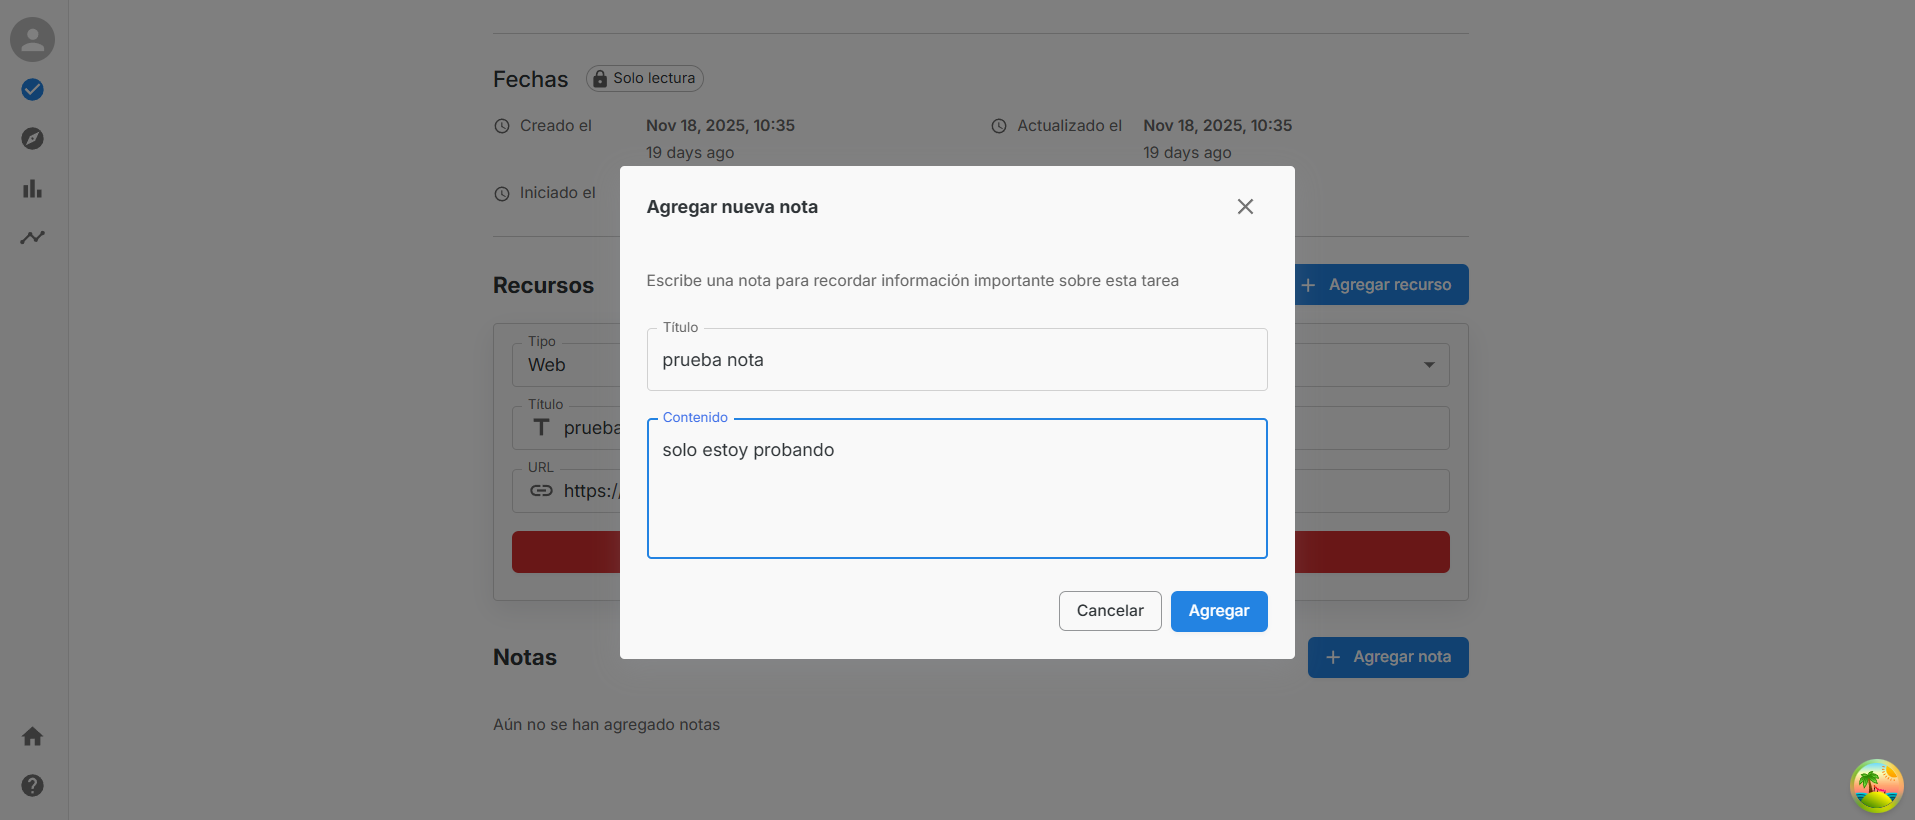
\includegraphics[width=0.95\textwidth]{Figuras/interfaces_AaA/tarea_agregar_nota.png}
\caption{Interfaz para agregar una nueva nota a una tarea.}
\label{fig:tarea-agregar-nota}
\end{figure}

\noindent\textit{Descripción.} La Figura~\ref{fig:tarea-agregar-nota} muestra el formulario utilizado para registrar una nota personal. El estudiante puede definir un título y un contenido, permitiendo documentar información útil para el avance de la tarea.

% (2) Listado y gestión de notas existentes
\begin{figure}[H]
\centering
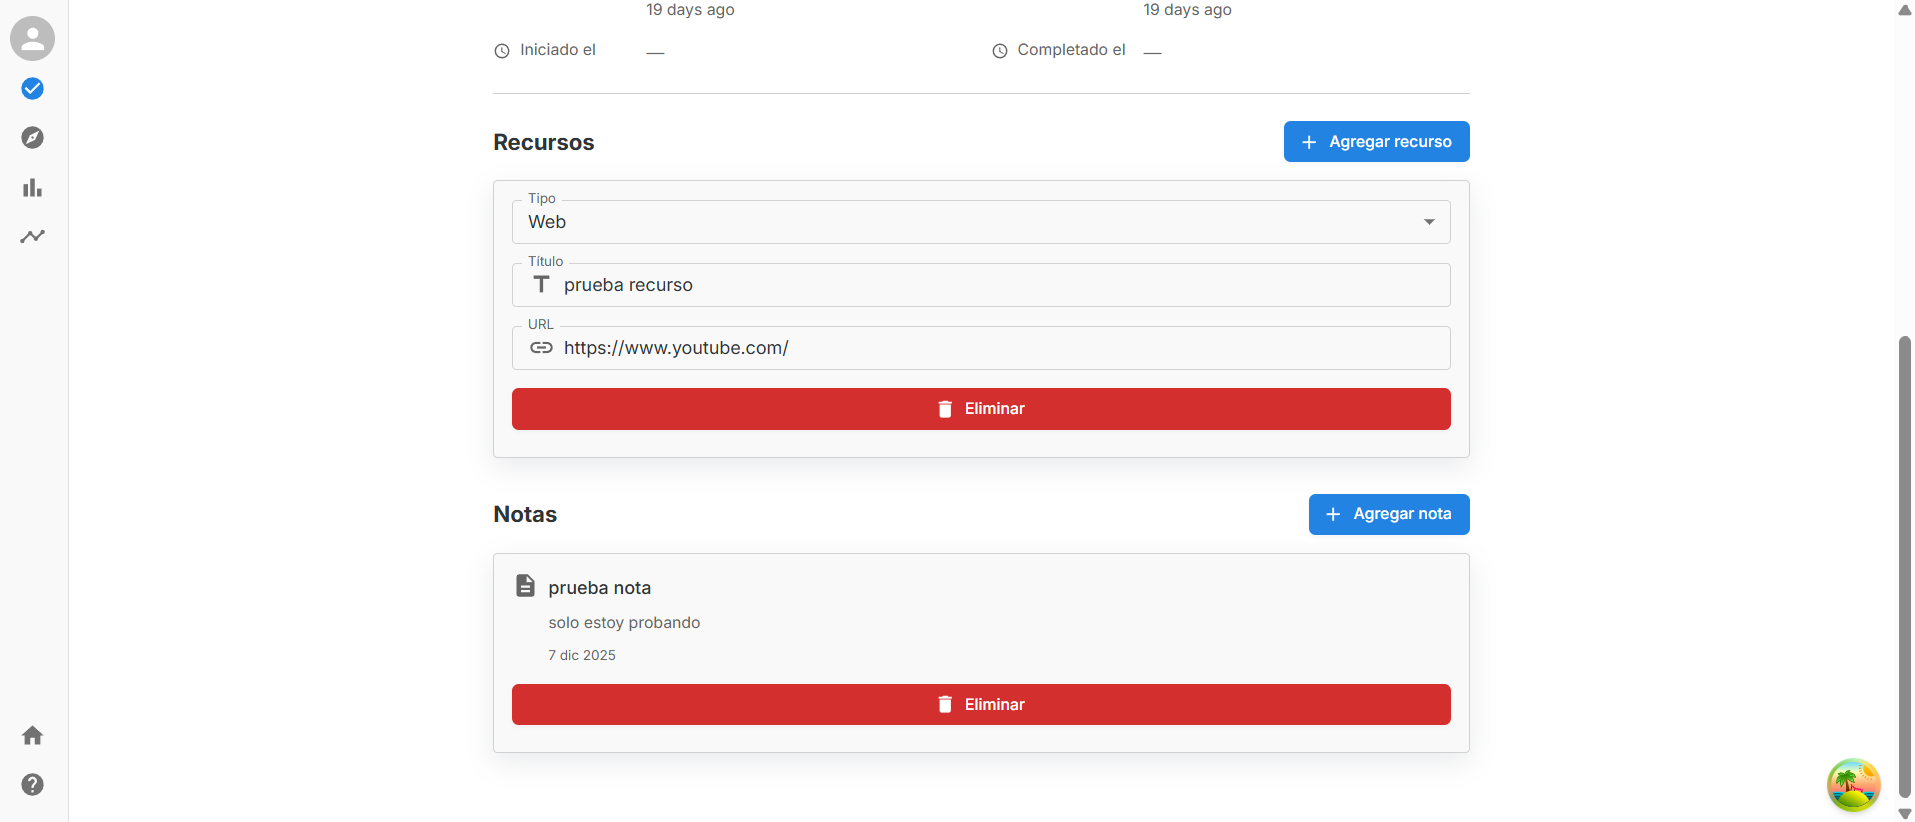
\includegraphics[width=0.95\textwidth]{Figuras/interfaces_AaA/tarea_listado_notas.png}
\caption{Listado de notas asociadas a una tarea, con opciones para su gestión.}
\label{fig:tarea-listado-notas}
\end{figure}

\noindent\textit{Descripción.} La Figura~\ref{fig:tarea-listado-notas} ilustra cómo las notas se presentan dentro del detalle de la tarea. Desde esta vista, el estudiante puede revisar o eliminar cada nota según requiera su proceso de estudio.

% -------------------------------------------------
\subsection*{Autoevaluación y reflexión guiada al finalizar una tarea}
% -------------------------------------------------

Al mover una tarea a la columna \textit{Hecho} dentro del tablero Kanban, el sistema presenta un formulario de reflexión orientado a promover la autorregulación del aprendizaje. Este formulario debe completarse para confirmar la finalización de la tarea; en caso de cancelarse, la tarea regresa automáticamente al estado previo, garantizando que toda actividad marcada como completada cuente con una reflexión asociada.

% (1) Reflexión: entorno e intención de aprendizaje
\begin{figure}[H]
\centering
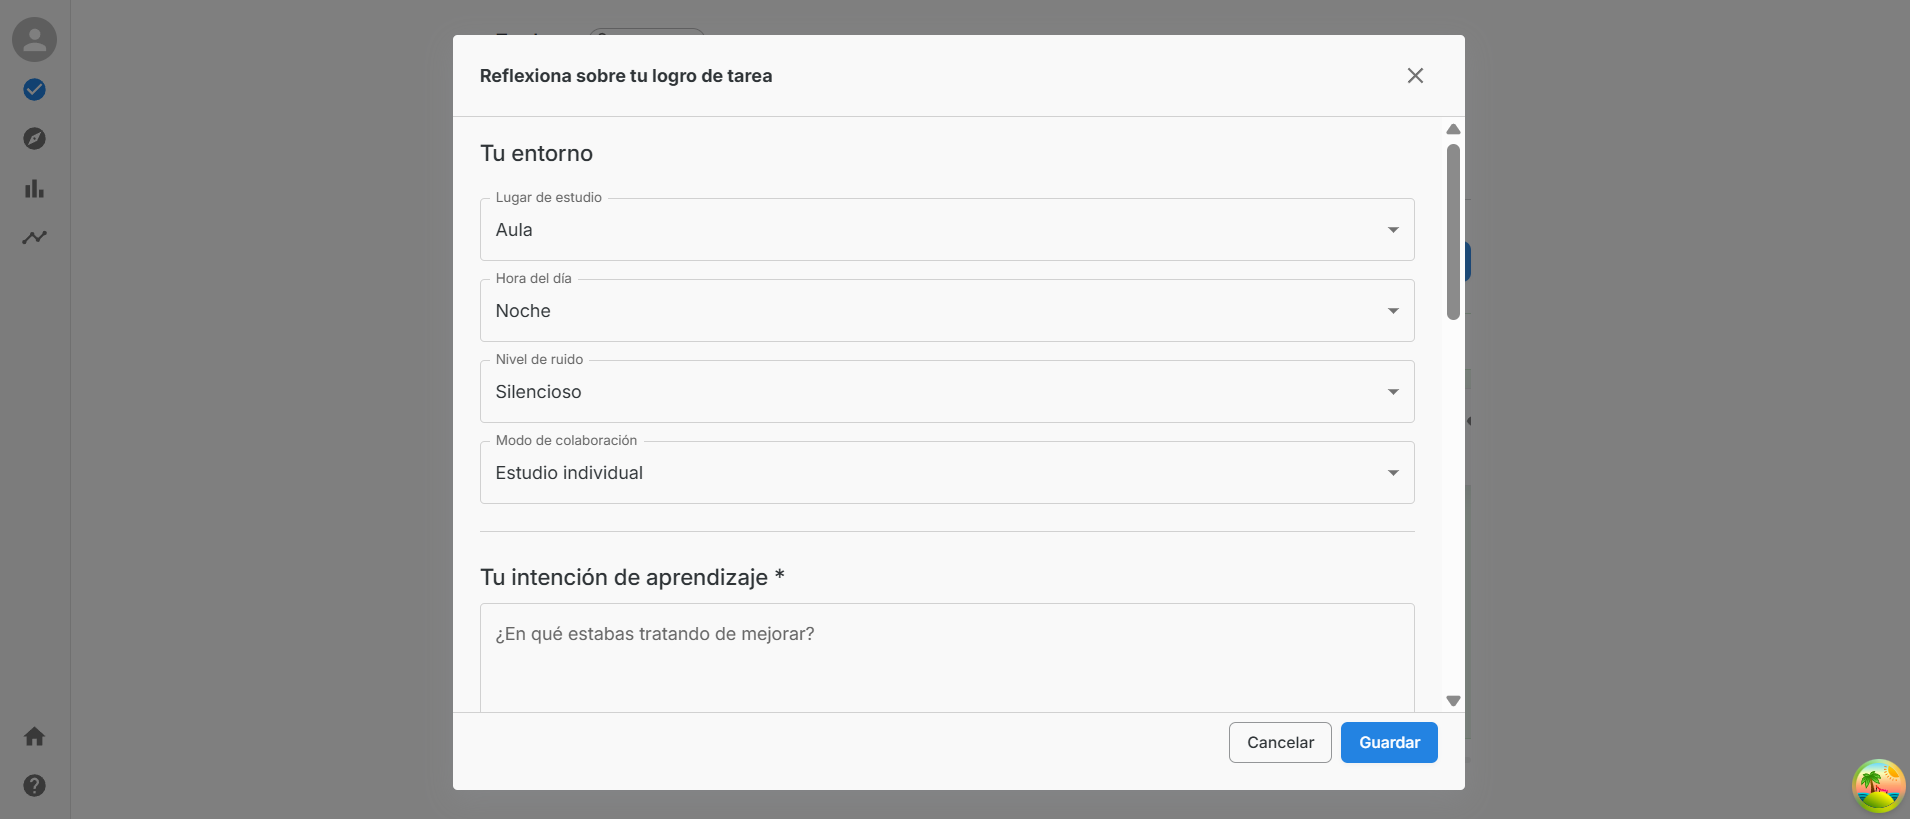
\includegraphics[width=0.95\textwidth]{Figuras/interfaces_AaA/reflexion_tarea_entorno.png}
\caption{Primera sección del formulario de reflexión: entorno y meta de aprendizaje.}
\label{fig:reflexion-tarea-entorno}
\end{figure}

\noindent\textit{Descripción.} La primera sección recopila información contextual sobre la sesión de estudio, incluyendo el lugar, la hora del día, el nivel de ruido y el modo de colaboración. También solicita la intención de aprendizaje asociada a la tarea, permitiendo al estudiante clarificar el propósito de su actividad.

% (2) Reflexión: experiencia durante la tarea
\begin{figure}[H]
\centering
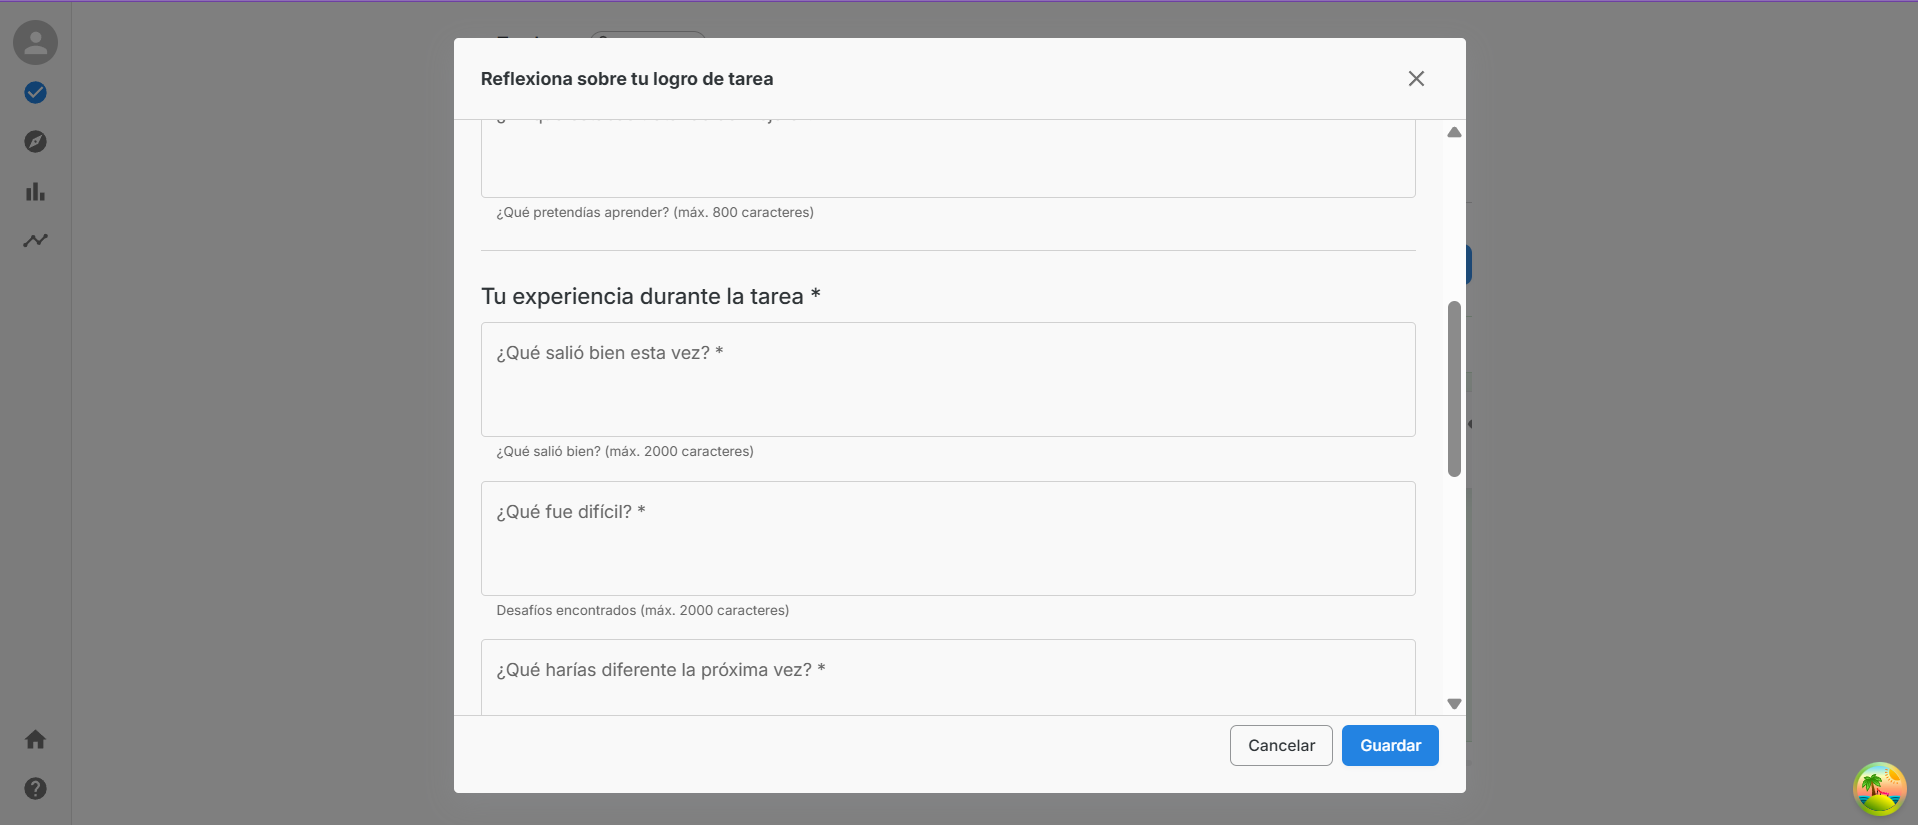
\includegraphics[width=0.95\textwidth]{Figuras/interfaces_AaA/reflexion_tarea_experiencia.png}
\caption{Segunda sección del formulario de reflexión: experiencia durante la tarea.}
\label{fig:reflexion-tarea-experiencia}
\end{figure}

\noindent\textit{Descripción.} En esta sección, el estudiante describe su experiencia al realizar la tarea, destacando qué salió bien, qué resultó difícil y qué acciones podría mejorar en futuras actividades. Este análisis favorece la toma de conciencia sobre el propio proceso de aprendizaje.

% (3) Reflexión: nivel de esfuerzo, concentración y estrategias
\begin{figure}[H]
\centering
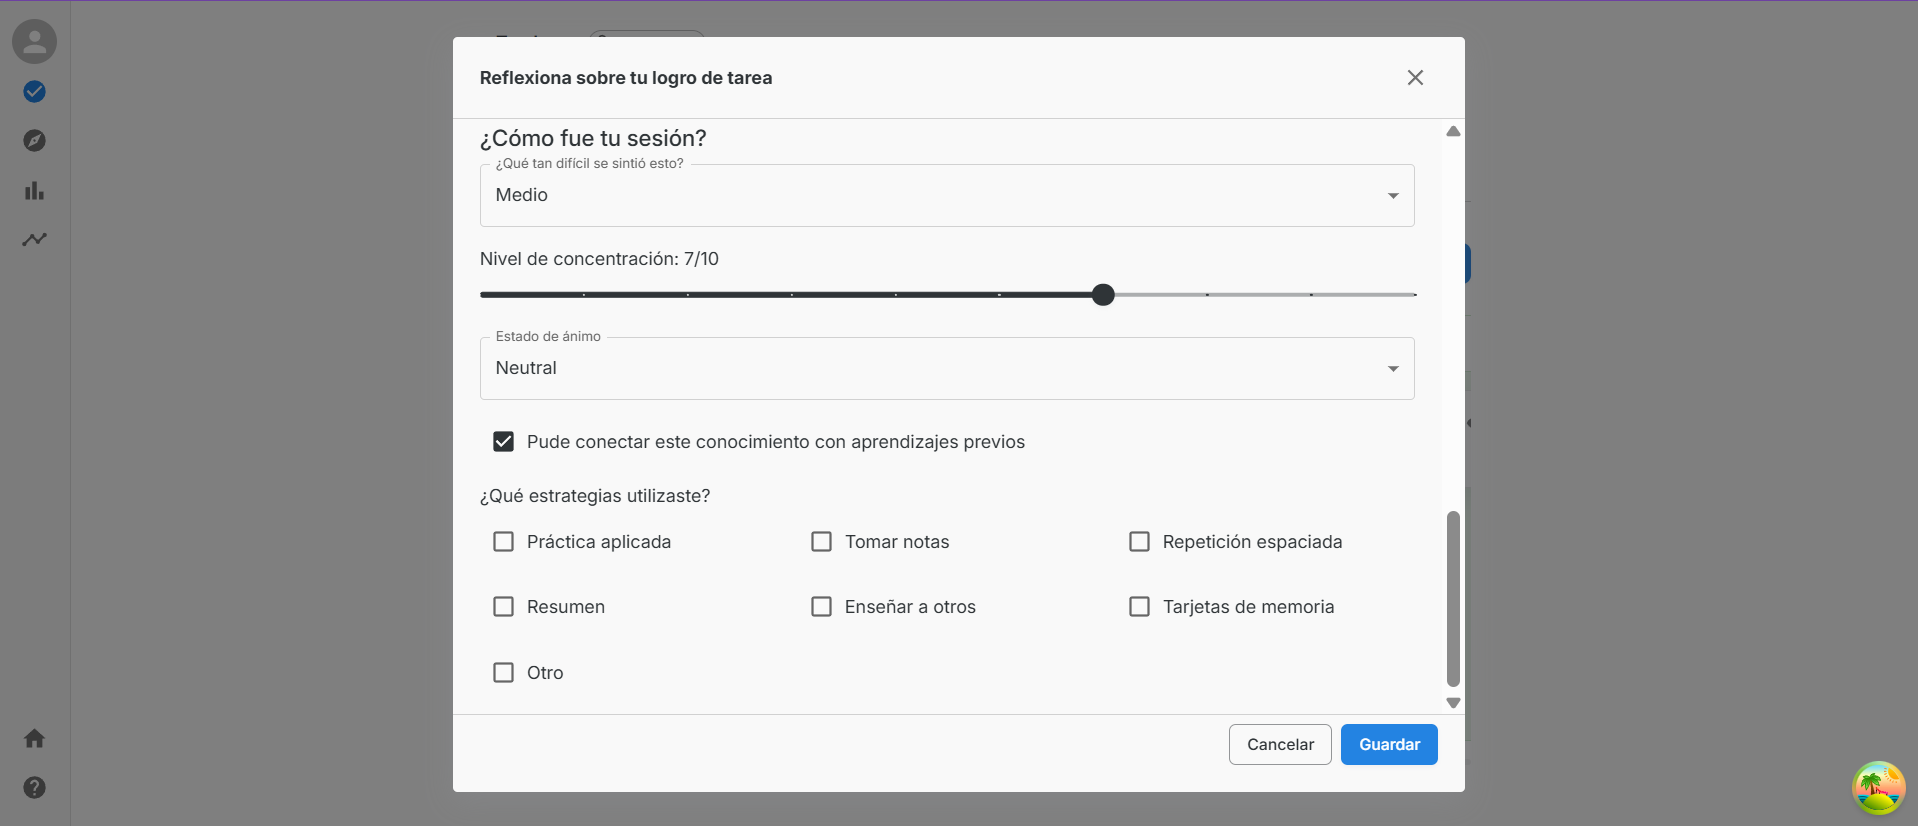
\includegraphics[width=0.95\textwidth]{Figuras/interfaces_AaA/reflexion_tarea_sesion.png}
\caption{Tercera sección del formulario de reflexión: nivel de esfuerzo, concentración, estado de ánimo y estrategias utilizadas.}
\label{fig:reflexion-tarea-sesion}
\end{figure}

\noindent\textit{Descripción.} La sección final incluye una valoración subjetiva sobre el nivel de dificultad, la concentración y el estado de ánimo del estudiante. Además, permite registrar las estrategias de aprendizaje utilizadas y si el nuevo conocimiento pudo conectarse con experiencias previas, reforzando así habilidades metacognitivas esenciales.

% -------------------------------------------------
\subsection*{Acceso a reportes de aprendizaje}
% -------------------------------------------------
% (1) Lista general de informes de aprendizaje
\begin{figure}[H]
\centering
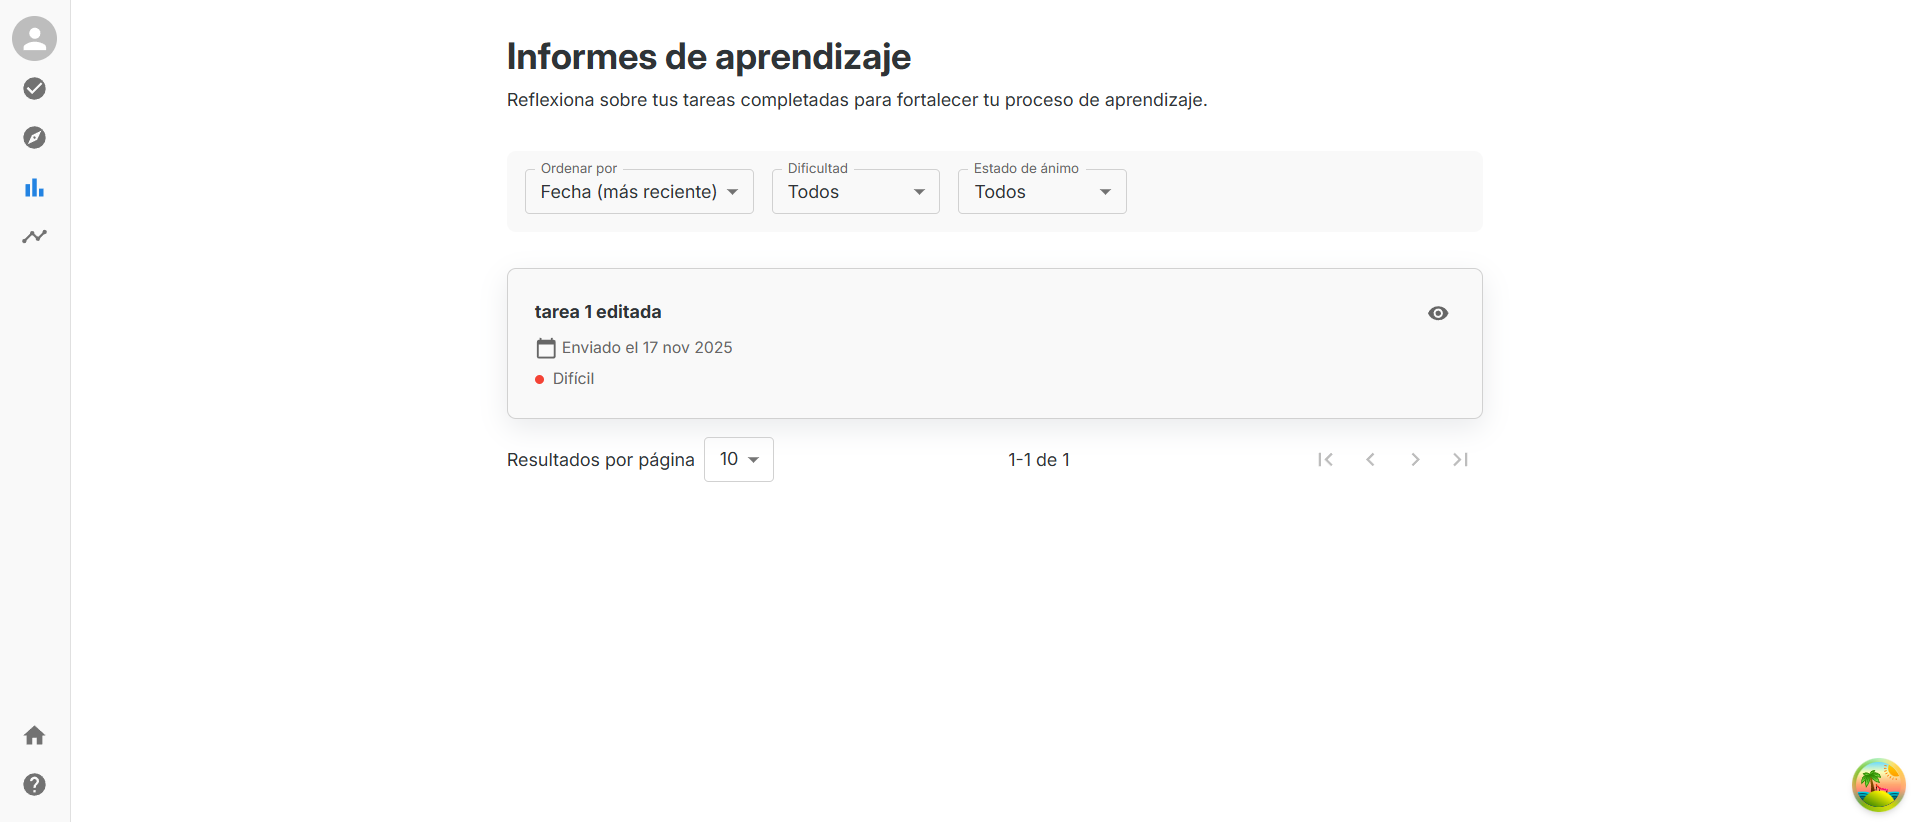
\includegraphics[width=0.95\textwidth]{Figuras/interfaces_AaA/reportes_lista_general.png}
\caption{Listado general de informes de aprendizaje, con opciones de ordenamiento y filtrado.}
\label{fig:reportes-lista-general}
\end{figure}

\noindent\textit{Descripción.} 
La vista inicial presenta todas las autoevaluaciones enviadas, permitiendo ordenar los reportes por fecha y aplicar filtros adicionales que facilitan la exploración del historial de aprendizaje.

% (2) Lista filtrada sin resultados
\begin{figure}[H]
\centering
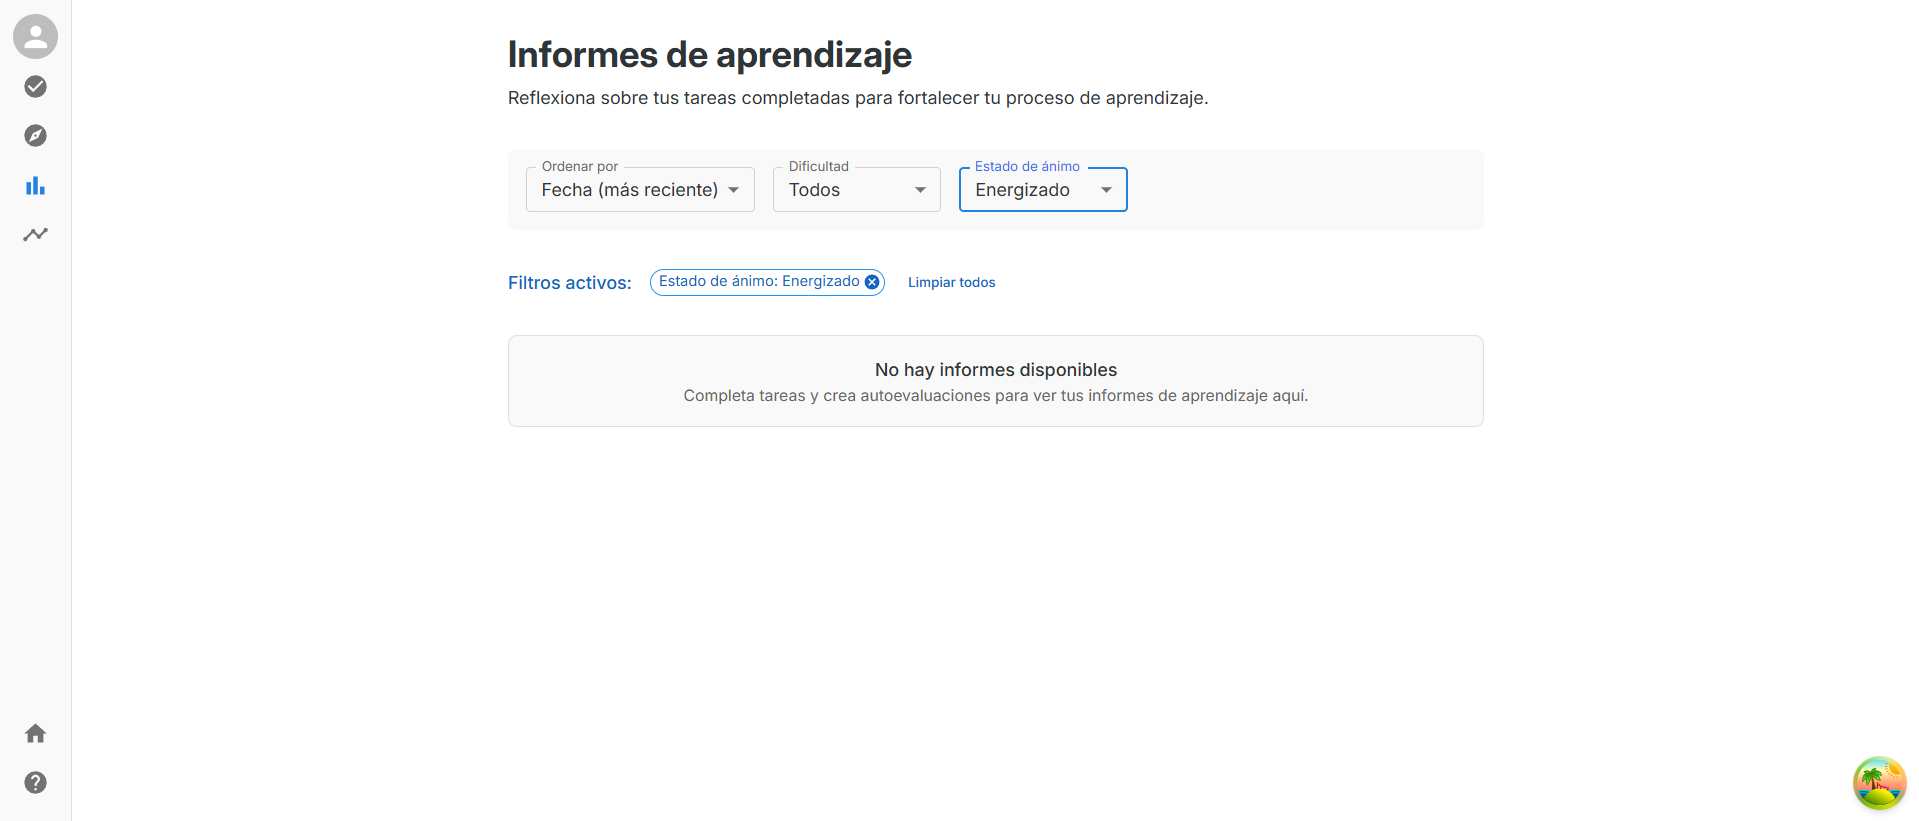
\includegraphics[width=0.95\textwidth]{Figuras/interfaces_AaA/reportes_sin_resultados.png}
\caption{Vista del módulo de reportes cuando los filtros aplicados no arrojan resultados.}
\label{fig:reportes-sin-resultados}
\end{figure}

\noindent\textit{Descripción.} 
Cuando ningún reporte coincide con los filtros seleccionados, el sistema informa al estudiante y lo invita a completar nuevas tareas y reflexiones para generar contenido en esta sección.

% (3) Vista detallada de un informe de aprendizaje
\begin{figure}[H]
\centering
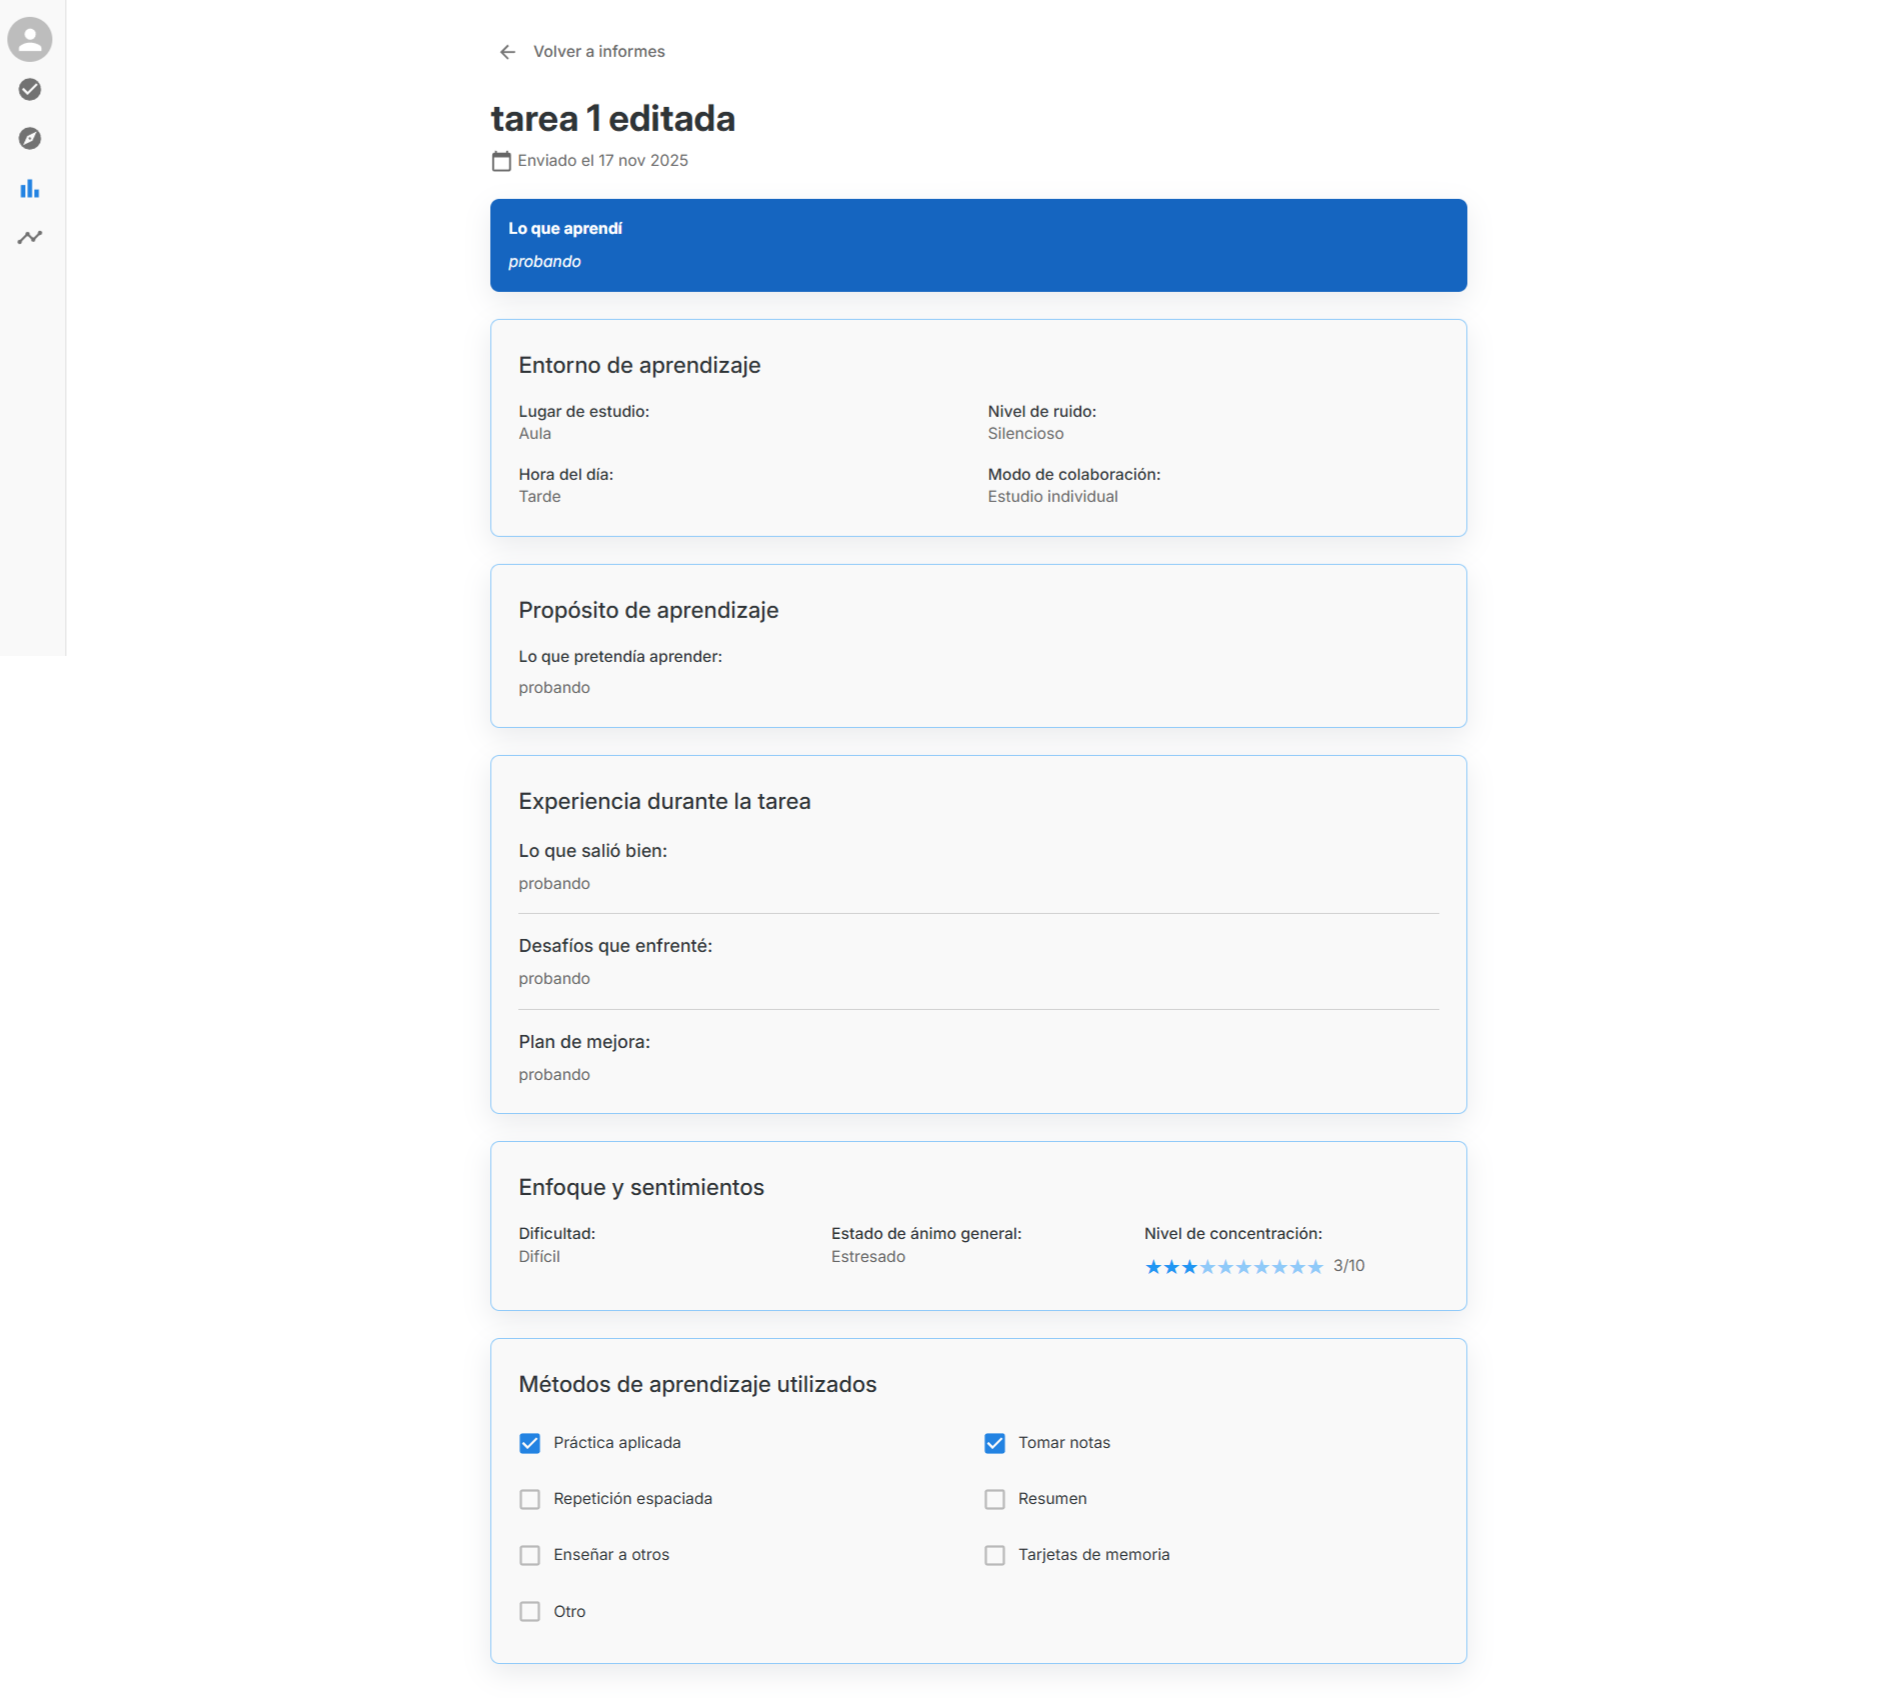
\includegraphics[width=0.95\textwidth]{Figuras/interfaces_AaA/reporte_detallado.png}
\caption{Vista detallada de un informe de aprendizaje asociado a una tarea completada.}
\label{fig:reporte-detallado}
\end{figure}

\noindent\textit{Descripción.} 
Cada informe consolida los datos registrados por el estudiante al finalizar la tarea. La vista incluye:  
(1) el entorno de estudio (lugar, nivel de ruido, colaboración y horario),  
(2) la intención de aprendizaje,  
(3) los aspectos logrados, desafíos encontrados y el plan de mejora,  
(4) indicadores complementarios como nivel de dificultad percibido, estado de ánimo y nivel de concentración,  
y (5) las estrategias de aprendizaje utilizadas.  

Esta estructura permite analizar la experiencia de estudio desde una perspectiva integral, facilitando el desarrollo de habilidades metacognitivas.

% -------------------------------------------------
\subsection*{Configuración de visibilidad de los planes de aprendizaje}
% -------------------------------------------------
% (1) Modal de configuración con visibilidad privada
\begin{figure}[H]
\centering
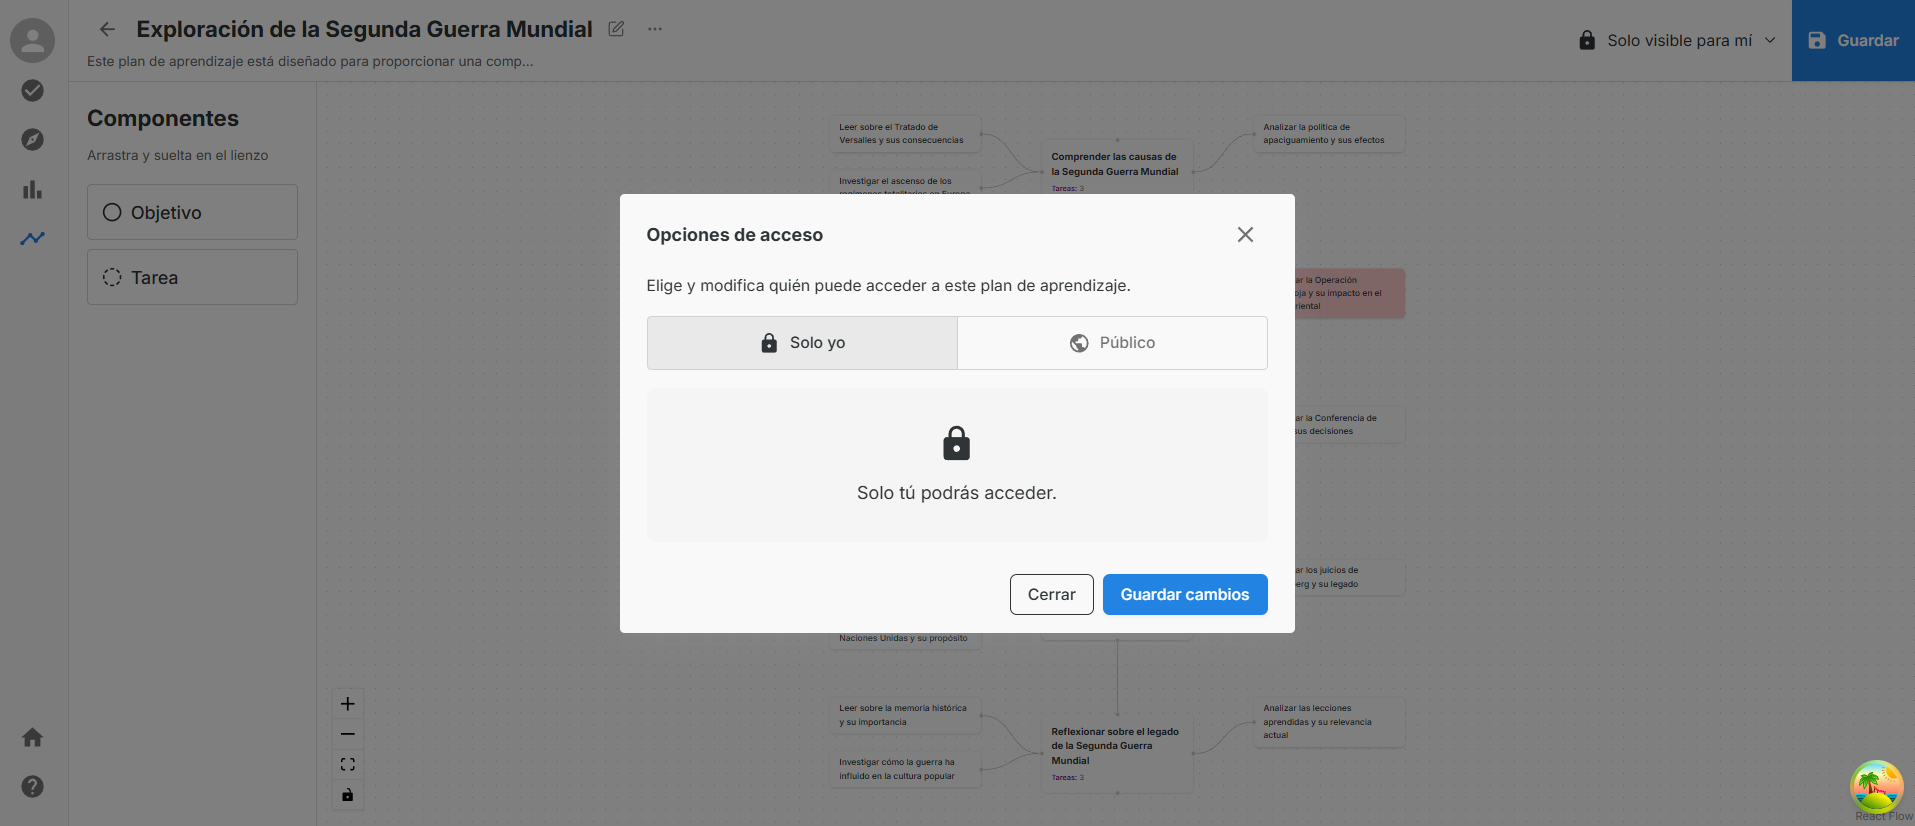
\includegraphics[width=0.95\textwidth]{Figuras/interfaces_AaA/visibilidad_privada.png}
\caption{Configuración de visibilidad de un plan de aprendizaje en modo privado.}
\label{fig:visibilidad-privada}
\end{figure}

\noindent\textit{Descripción.} En el modo \textit{Solo yo}, el plan permanece accesible únicamente para el estudiante, asegurando privacidad total durante su creación o revisión.

% (2) Modal de configuración con visibilidad pública mediante enlace
\begin{figure}[H]
\centering
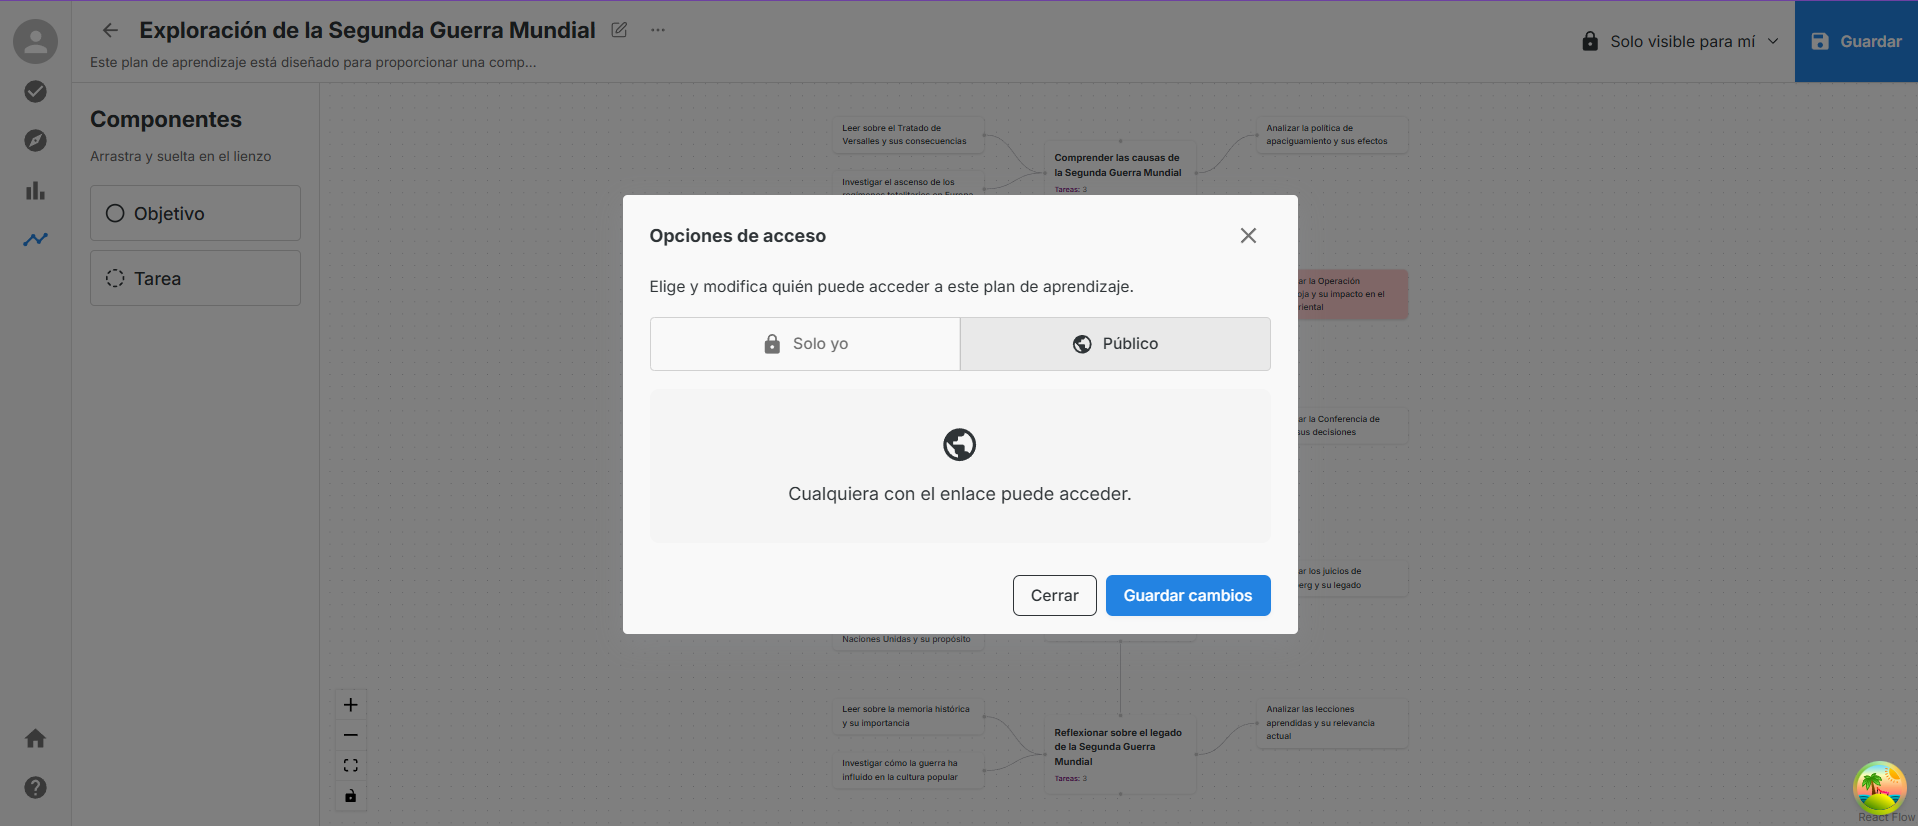
\includegraphics[width=0.95\textwidth]{Figuras/interfaces_AaA/visibilidad_publica.png}
\caption{Configuración de visibilidad que habilita el acceso público mediante enlace.}
\label{fig:visibilidad-publica-enlace}
\end{figure}

\noindent\textit{Descripción.} Al seleccionar la opción \textit{Público}, el sistema permite compartir el plan con cualquier persona que posea el enlace correspondiente, lo que facilita su difusión y reutilización en actividades colaborativas o procesos formativos.

% -------------------------------------------------
% Anexo D. Interfaces del módulo de Escucha Activa
% -------------------------------------------------
\section*{Anexo D. Interfaces del módulo de Escucha Activa}
\addcontentsline{toc}{section}{Anexo D. Interfaces del módulo de Escucha Activa}
\label{anexo:interfaces_escucha_activa}

Este anexo presenta las interfaces asociadas al módulo de escucha activa. Las figuras ilustran los distintos momentos de interacción del estudiante durante una sesión de juego: la configuración inicial, la selección y gestión de sesiones, el desarrollo de cada ronda y la revisión del desempeño global.

% -------------------------------------------------
\subsection*{Configuración inicial de la sesión de juego}
% -------------------------------------------------

\begin{figure}[H]
\centering
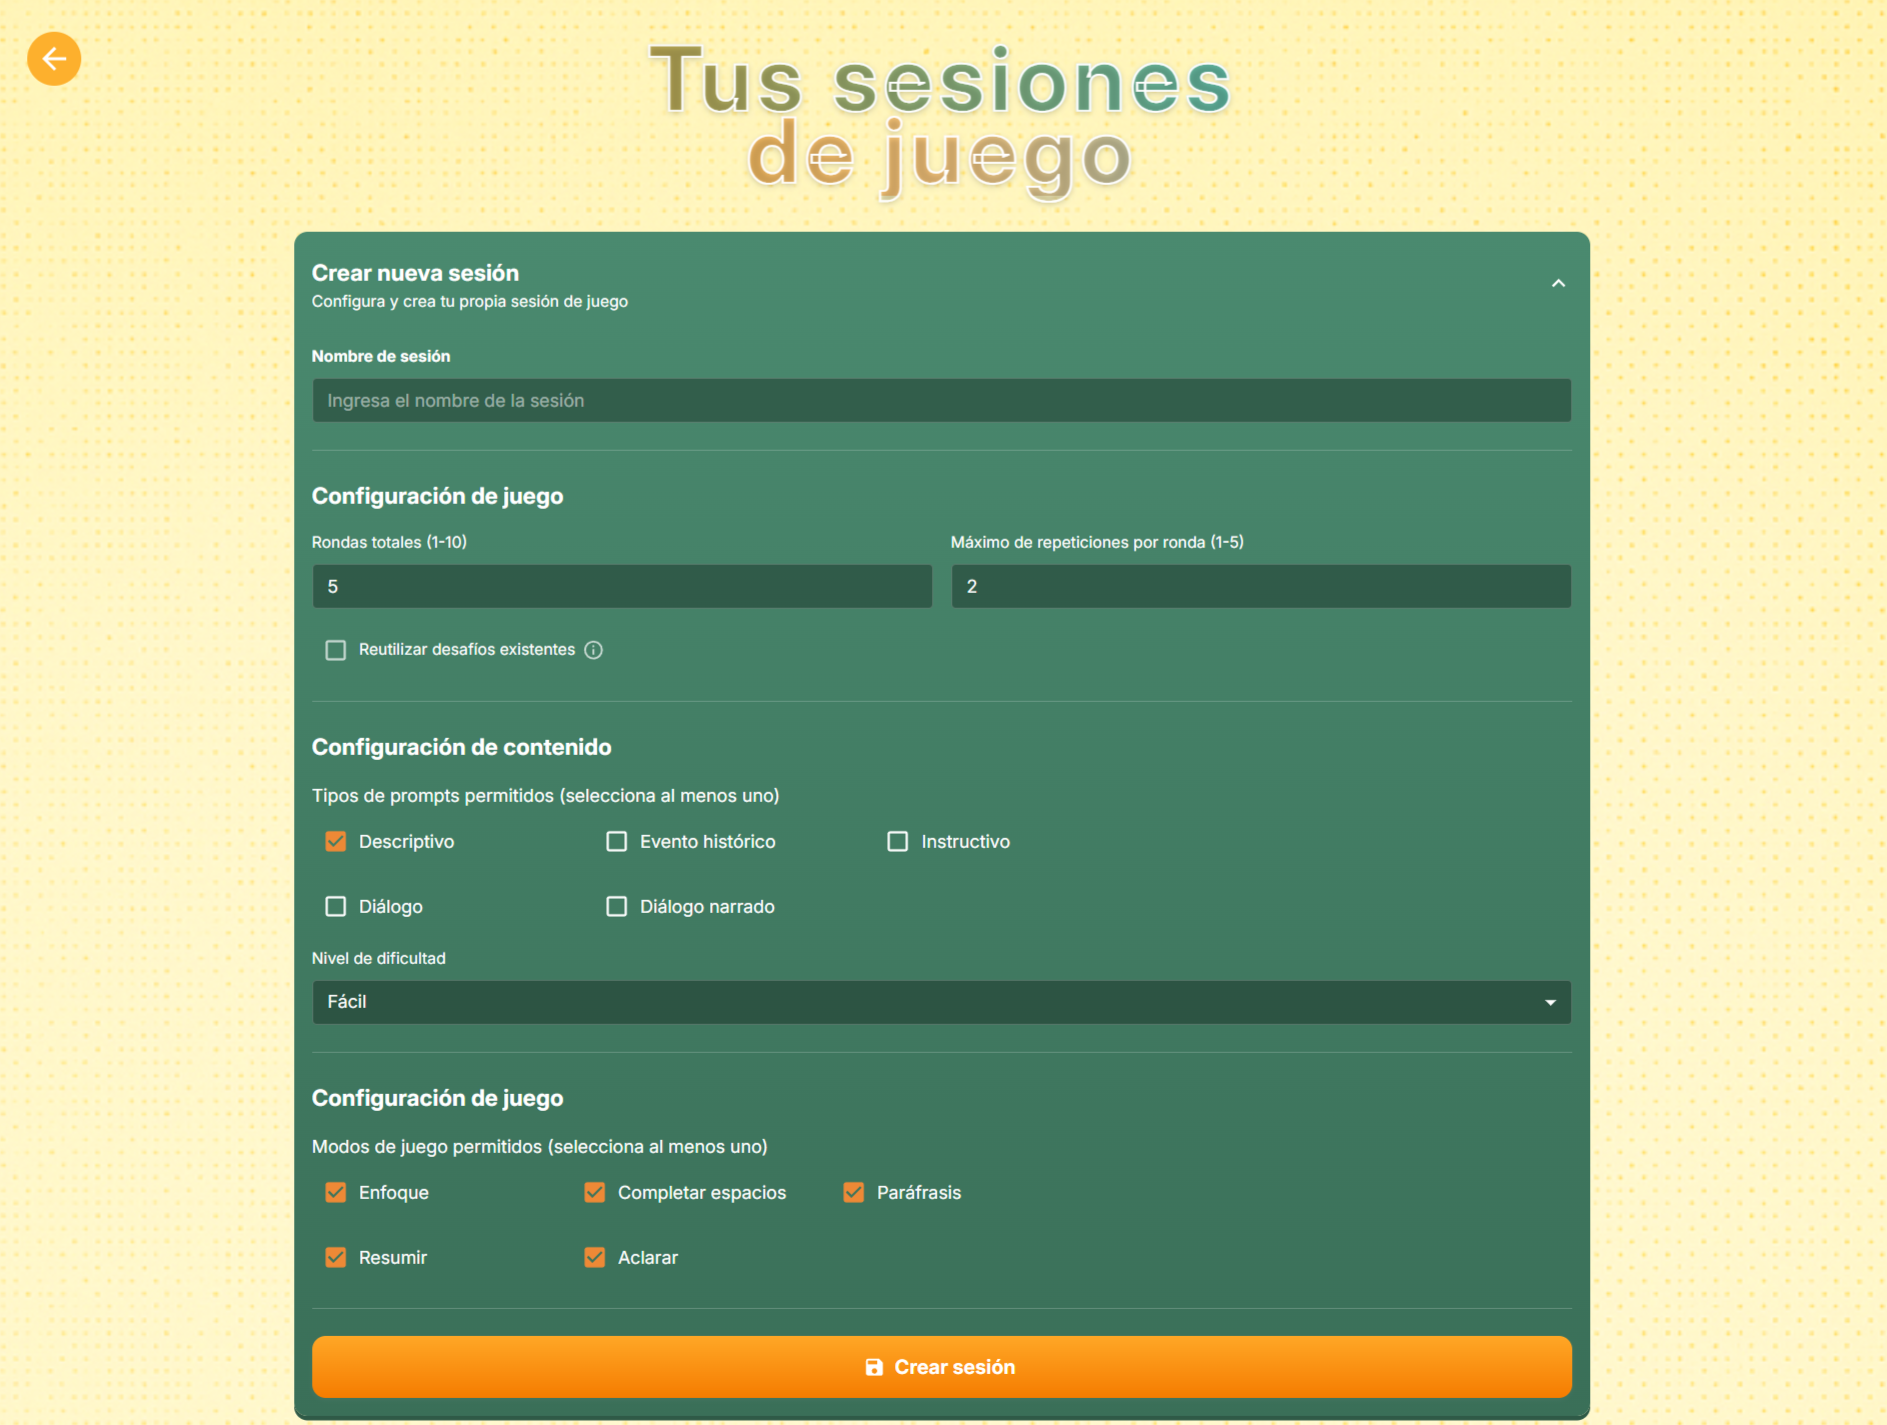
\includegraphics[width=0.95\textwidth]{Figuras/interfaces_EA/ea_crear_sesion.png}
\caption{Interfaz para la creación y configuración de una nueva sesión de juego.}
\label{fig:ea-configuracion-sesion}
\end{figure}

\noindent\textit{Descripción.}
Antes de iniciar una sesión, el estudiante define parámetros como el número total de rondas, el máximo de repeticiones por ronda, los tipos de prompts permitidos y los modos de juego habilitados. También puede decidir si desea reutilizar desafíos previamente generados.

% -------------------------------------------------
\subsection*{Listado de sesiones de juego}
% -------------------------------------------------

\begin{figure}[H]
\centering
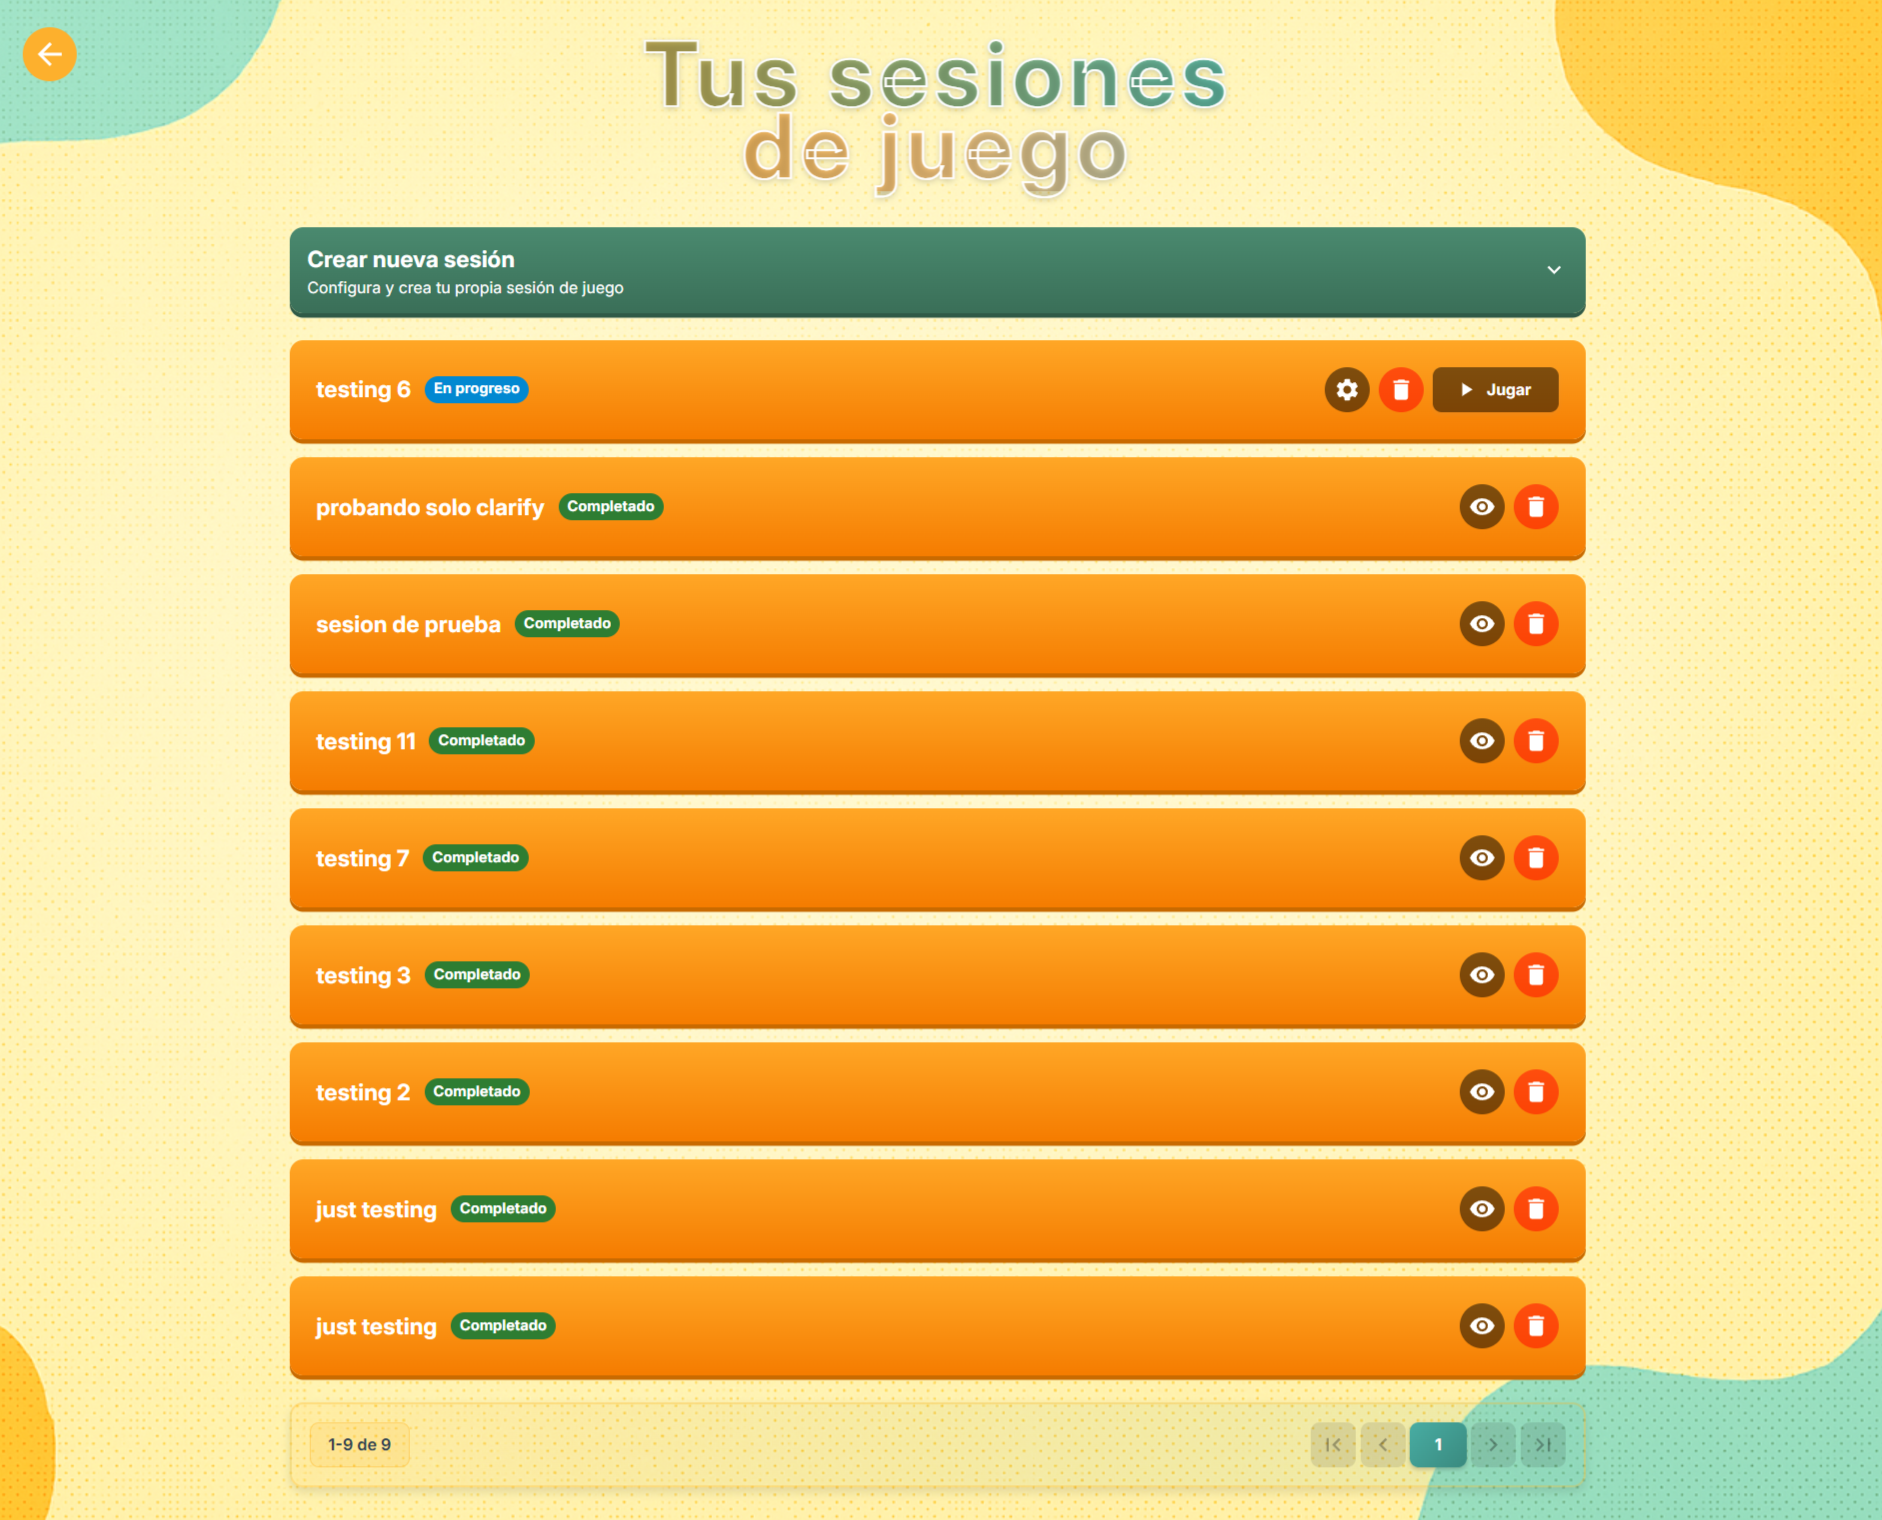
\includegraphics[width=0.95\textwidth]{Figuras/interfaces_EA/ea_listado_sesiones.png}
\caption{Listado de sesiones creadas por el estudiante, con opciones para gestionarlas o reanudar el juego.}
\label{fig:ea-listado-sesiones}
\end{figure}

\noindent\textit{Descripción.}
La vista principal muestra todas las sesiones creadas, indicando su estado (\textit{En progreso} o \textit{Completado}). Desde esta sección, el estudiante puede iniciar, continuar, revisar o eliminar sesiones existentes.

% -------------------------------------------------
\subsection*{Interacción dentro de una ronda de juego}
% -------------------------------------------------

\begin{figure}[H]
\centering
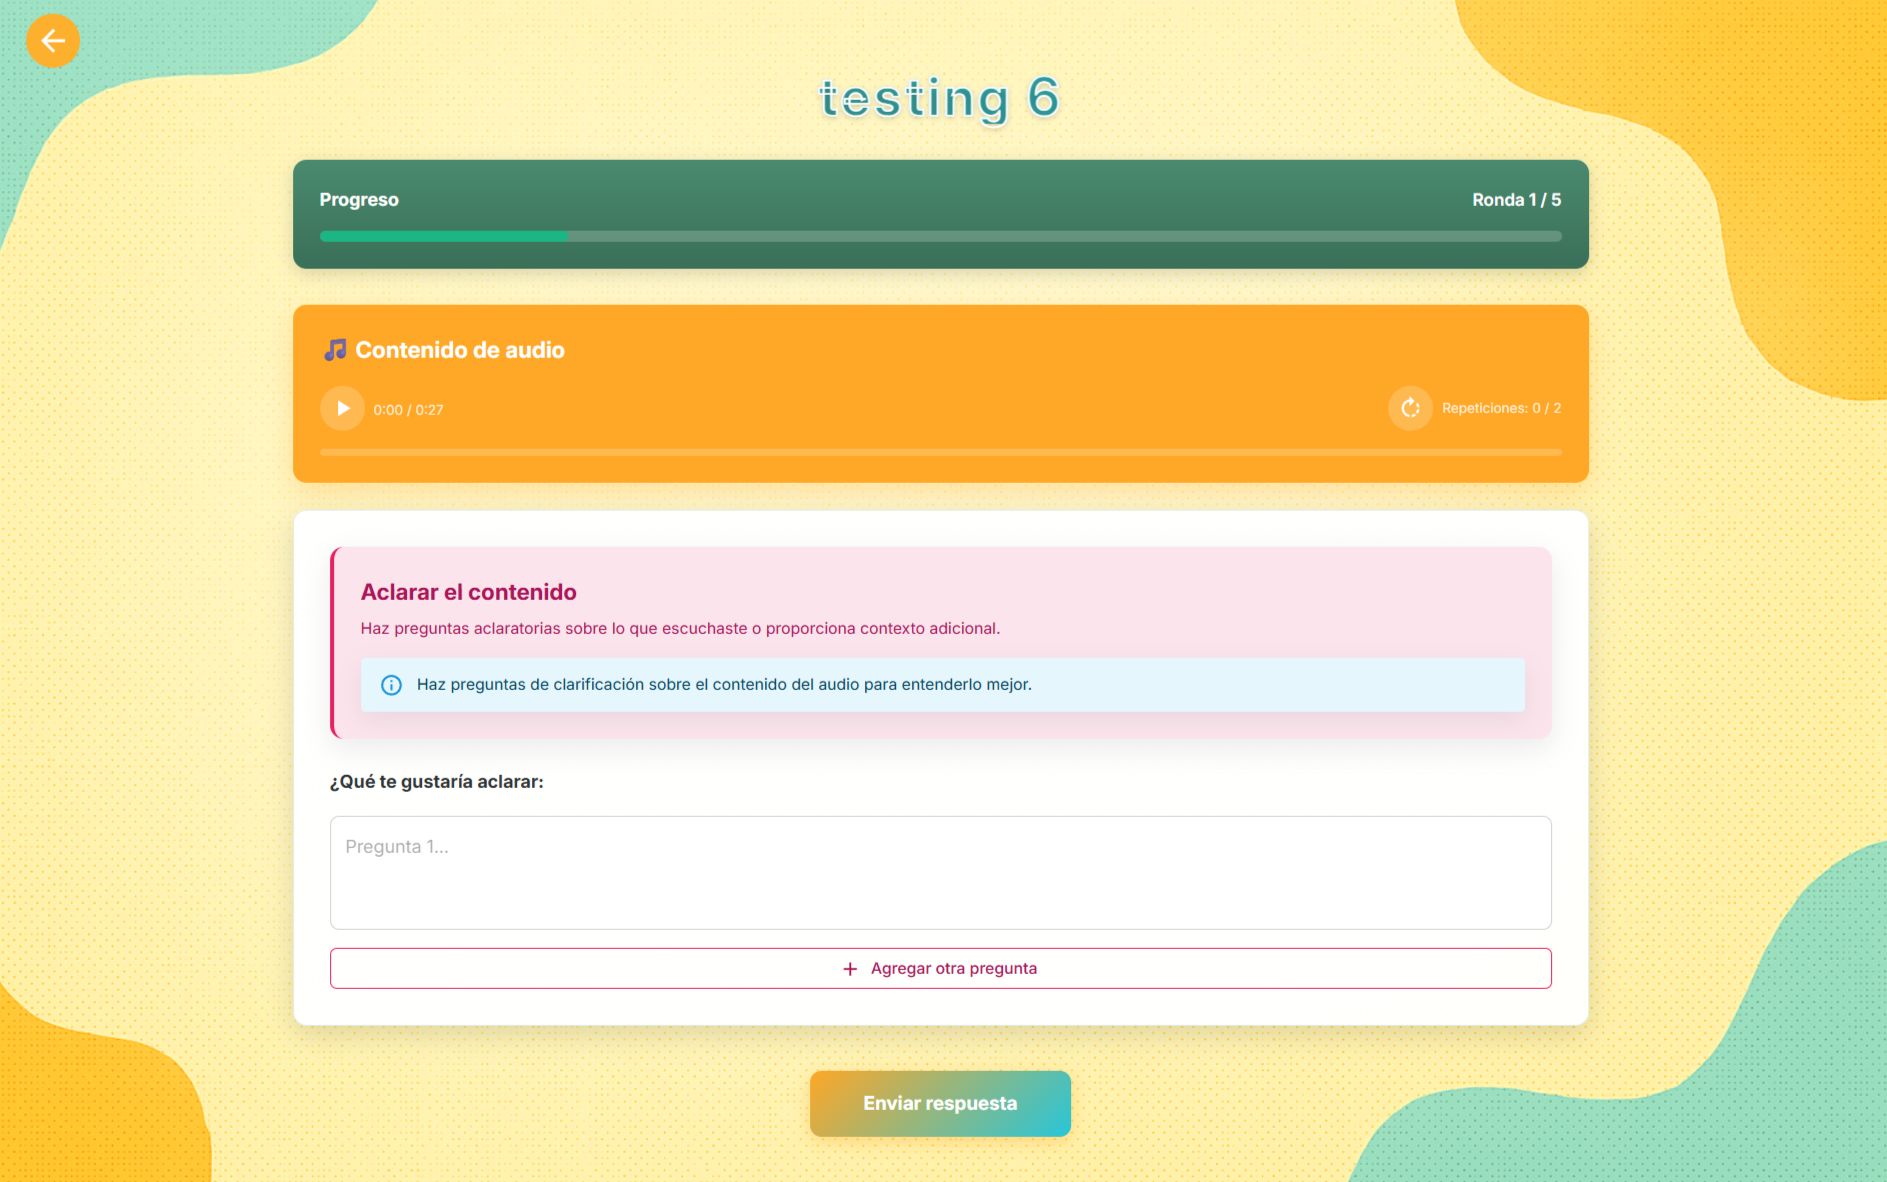
\includegraphics[width=0.95\textwidth]{Figuras/interfaces_EA/ea_ronda_juego.png}
\caption{Interfaz de una ronda activa, mostrando el audio, el conteo de repeticiones y el ejercicio asociado al modo de juego.}
\label{fig:ea-ronda}
\end{figure}

\noindent\textit{Descripción.}
Cada ronda presenta el clip de audio generado por el sistema, el número de repeticiones de reproducción utilizadas y disponibles, y el ejercicio correspondiente al modo de juego asignado (p. ej., aclarar, resumir, completar espacios). El estudiante puede volver a escuchar el audio dentro del límite permitido antes de responder, y posteriormente envía su respuesta mediante el formulario presentado.


% -------------------------------------------------
\subsection*{Evaluación y retroalimentación por ronda}
% -------------------------------------------------

\begin{figure}[H]
\centering
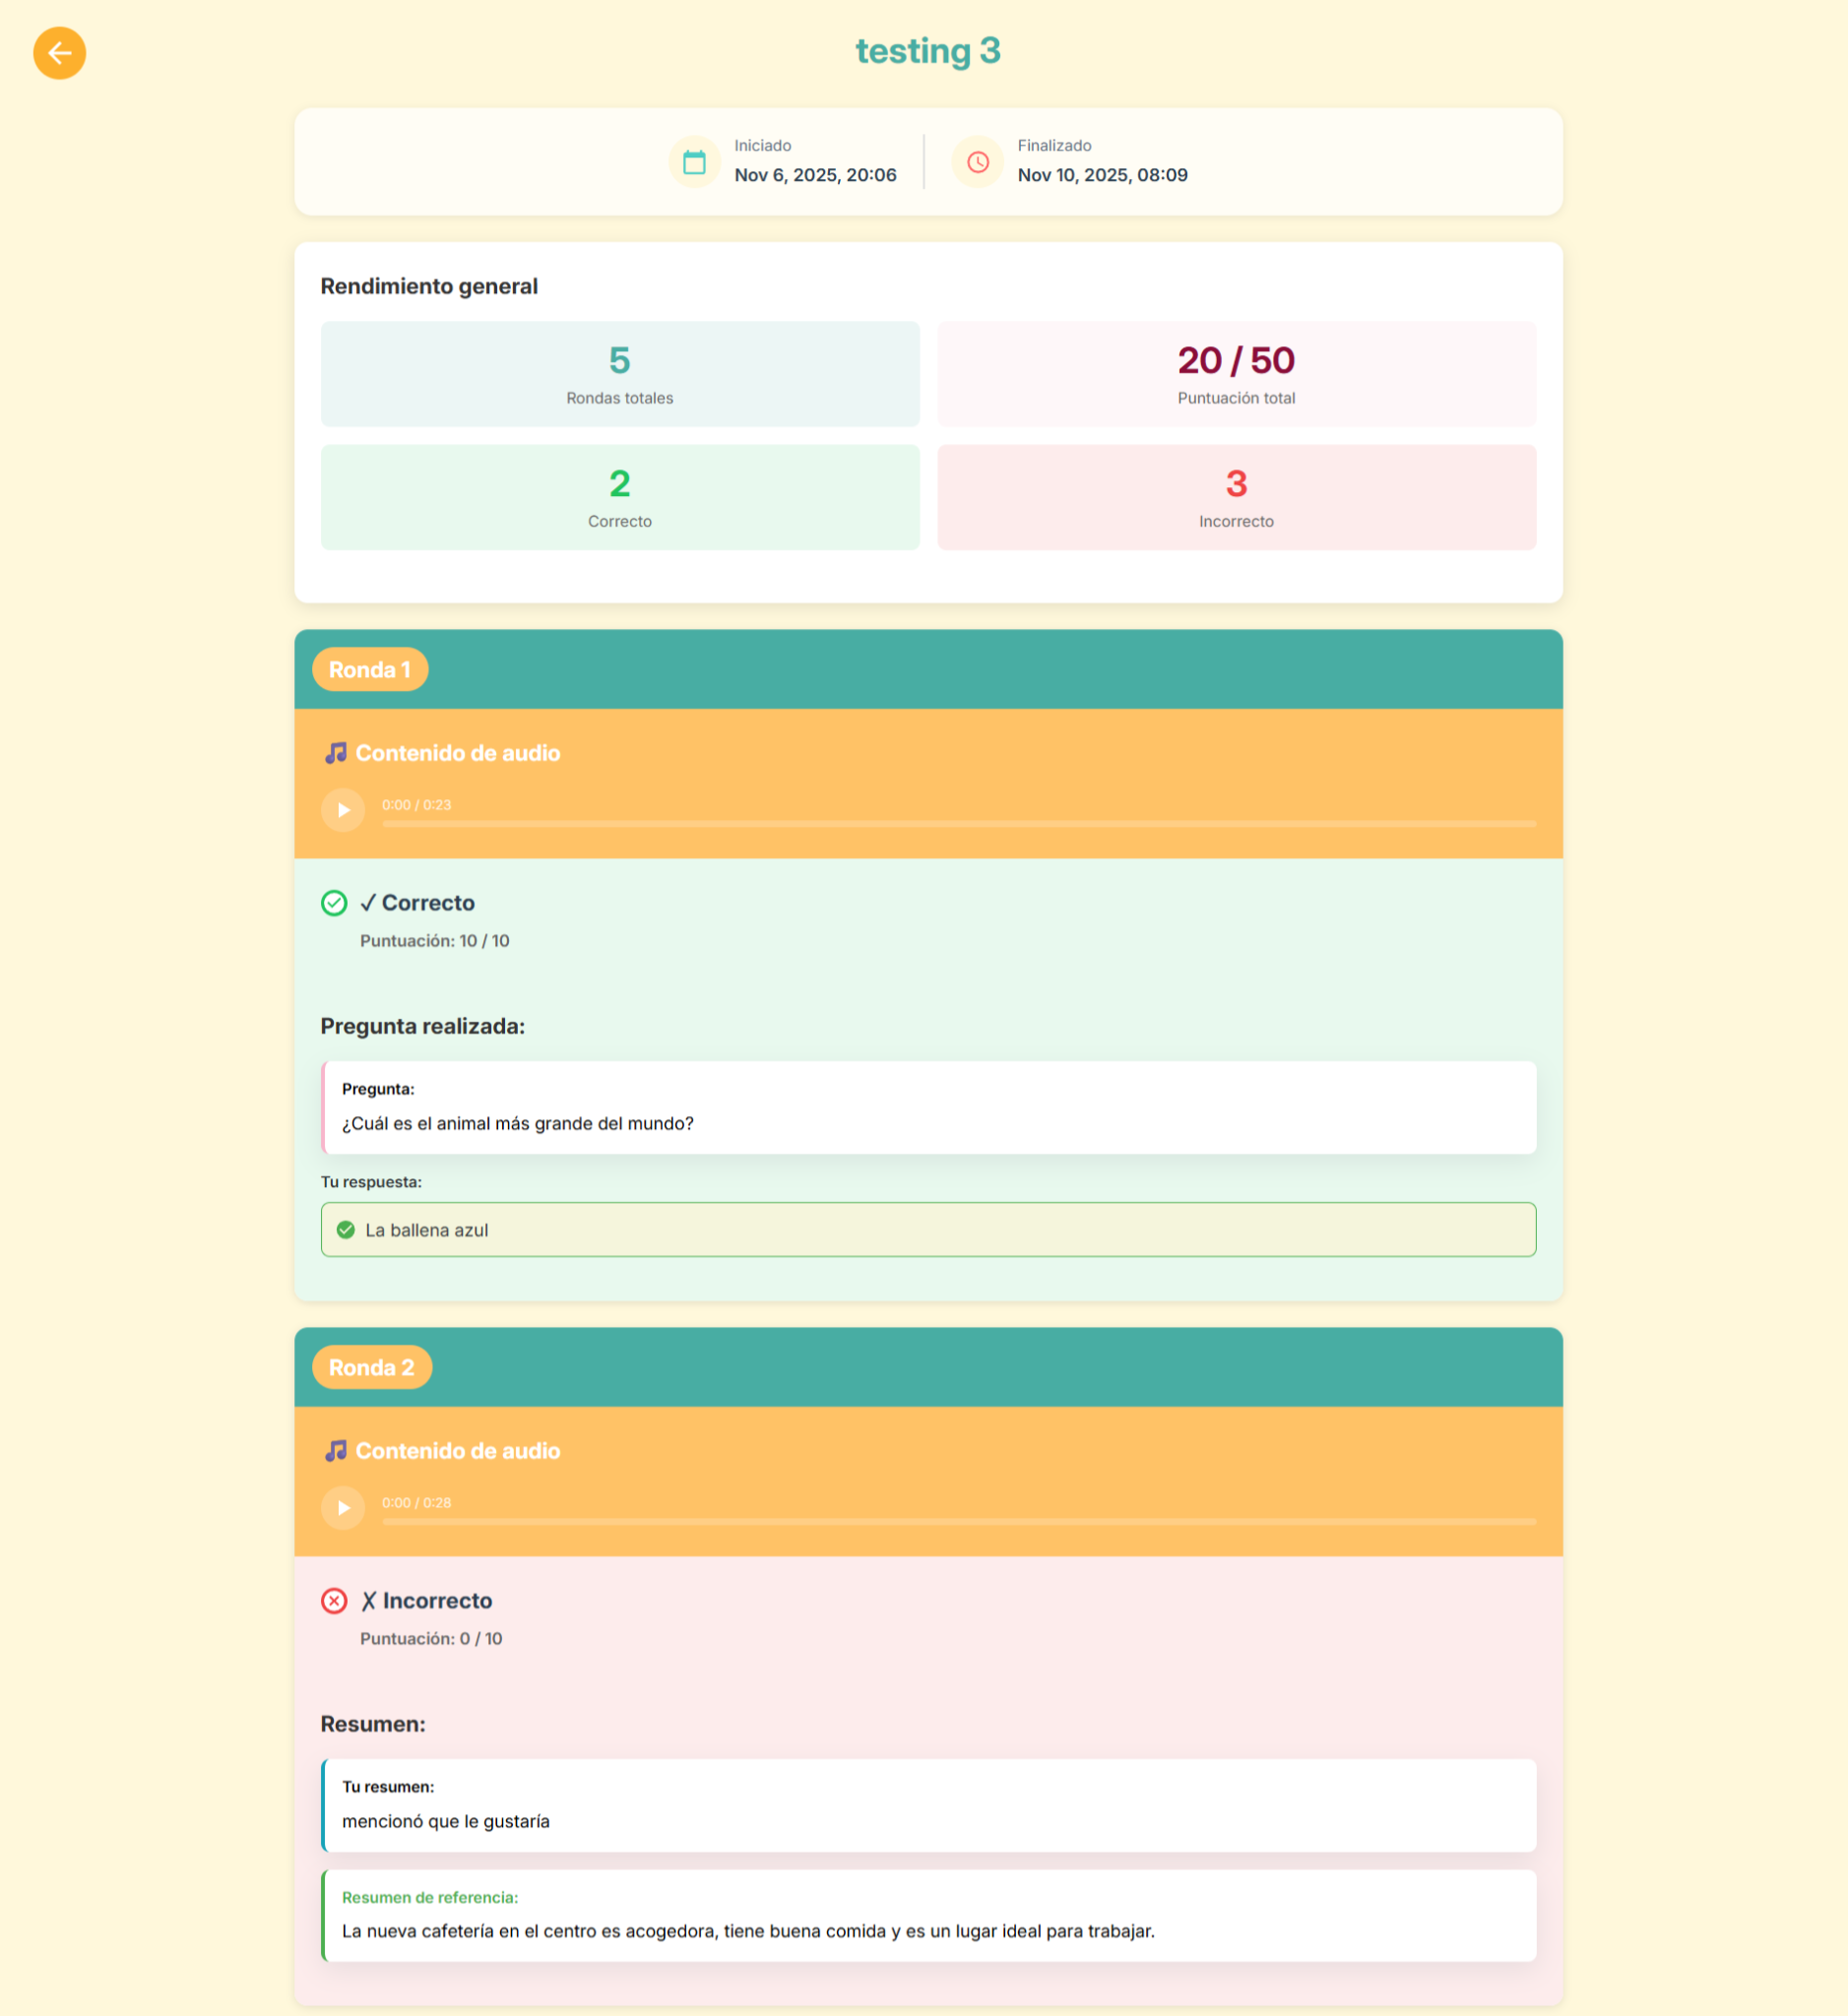
\includegraphics[width=0.95\textwidth]{Figuras/interfaces_EA/ea_reporte_sesion.png}
\caption{Reporte general de una sesión completada, con el desglose de rondas y sus resultados.}
\label{fig:ea-reporte-sesion}
\end{figure}

\noindent\textit{Descripción.}
Una vez finalizada la sesión, se presenta un informe detallado que incluye el número total de rondas, la puntuación acumulada, las respuestas correctas e incorrectas y un desglose completo de cada ronda. Cada bloque muestra el audio utilizado, la respuesta enviada, la evaluación otorgada y (cuando aplica) la comparación con la respuesta o referencia generada por el sistema.

% -------------------------------------------------
\subsection*{Detalle de ejercicios según el modo de juego}
% -------------------------------------------------

\noindent Los ejercicios correspondientes a los modos de juego \textit{Enfoque}, \textit{Completar espacios}, \textit{Paráfrasis}, \textit{Resumen} y \textit{Aclarar} se presentan directamente dentro de la interfaz de cada ronda. Dado que estas actividades se integran de manera contextualizada en la vista de ronda ya ilustrada en la Figura~\ref{fig:ea-ronda}, no se incluyen capturas adicionales. Cada ejercicio adapta dinámicamente su formato al tipo de interacción requerido por el modo de juego.



% -------------------------------------------------
% Anexo E. Elementos de gamificación implementados en el prototipo
% -------------------------------------------------
\section*{Anexo E. Elementos de gamificación implementados en el prototipo}
\addcontentsline{toc}{section}{Anexo E. Elementos de gamificación implementados en el prototipo}
\label{anexo:gamificacion}

La siguiente tabla presenta una comparación entre los elementos de gamificación descritos por Watini y Setyowati (2023) y su implementación dentro de los módulos \textit{Aprender a Aprender} y \textit{Escucha Activa} del prototipo desarrollado. Esta tabla complementa la descripción teórica incluida en el capítulo correspondiente al objetivo específico 3 y permite visualizar, de manera sintética, la relación entre la fundamentación académica y las funcionalidades implementadas.

\vspace{0.4cm}

\begin{table}[H]
\centering
\footnotesize
\setlength{\tabcolsep}{6pt}
\renewcommand{\arraystretch}{1.4}
\begin{tabular}{|p{3.2cm}|p{3.2cm}|p{4.2cm}|p{4.2cm}|}
\hline
\textbf{Elemento de gamificación} & \textbf{Fundamento (Watini \& Setyowati, 2023)} & \textbf{Implementación en Aprender a Aprender} & \textbf{Implementación en Escucha Activa} \\
\hline

\textbf{Progresión por niveles} &
Progresión incremental mediante unidades pequeñas de avance. &
Estructura metas–objetivos–tareas que permite avanzar gradualmente. &
Rondas secuenciales que se desbloquean al completar la anterior. \\
\hline

\textbf{Retroalimentación inmediata} &
La motivación aumenta con feedback instantáneo tras una acción. &
Autoevaluaciones por tarea; actualización del estado en el Kanban. &
Puntuación inmediata por ronda; comparación entre respuestas y criterios. \\
\hline

\textbf{Indicadores visuales de progreso} &
El progreso visible guía el comportamiento y mantiene el compromiso. &
Estados Kanban: Por hacer, En progreso, En pausa, Completado. &
Barra de progreso por ronda y resumen final de desempeño. \\
\hline

\textbf{Dificultad ajustada} &
Los desafíos deben ser equilibrados para evitar frustración. &
Complejidad variable de objetivos y tareas según el plan del estudiante. &
Configuración del nivel de dificultad (longitud del audio, complejidad semántica, modo de juego). \\
\hline

\textbf{Personalización y agencia} &
Permitir decisiones incrementa el sentido de control y la motivación. &
Creación, edición y copia de planes; personalización del roadmap. &
Configuración de rondas, prompts, dificultad y reutilización de desafíos. \\
\hline

\textbf{Anticipación del siguiente paso} &
Mantener al usuario en flujo reduce el abandono. &
Indicaciones para la siguiente tarea y objetivo dentro del roadmap. &
Transiciones automáticas entre rondas y vista previa del avance. \\
\hline

\textbf{Socialización indirecta} &
La percepción de comunidad actúa como motivador. &
Exploración de planes públicos creados por otros estudiantes. &
No aplica de forma directa; el enfoque es individual. \\
\hline

\end{tabular}
\caption{Relación entre elementos de gamificación y su implementación en el prototipo.}
\label{table:gamification-elements}
\end{table}
% -------------------------------------------------
% Anexo F. Diagramas de arquitectura del backend
% -------------------------------------------------
\section*{Anexo F. Diagramas de arquitectura del backend}
\addcontentsline{toc}{section}{Anexo F. Diagramas de arquitectura del backend}
\label{anexo:diagramas_backend}

% -------------------------------------------------
\subsection*{F.1 Gestión de metas de aprendizaje}
% -------------------------------------------------

\begin{figure}[H]
\centering
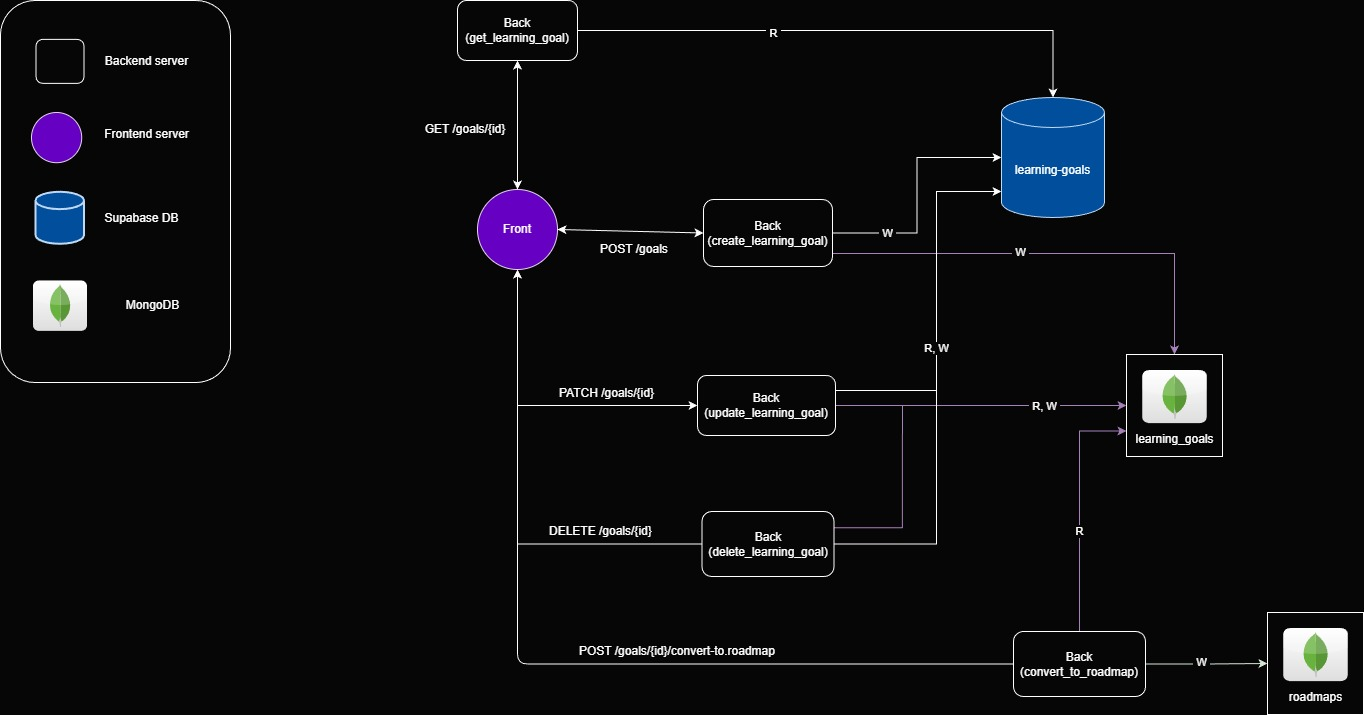
\includegraphics[width=\textwidth]{Figuras/arquitecture_diagrams/learning_goals.jpg}
\caption{Diagrama de arquitectura para la gestión de metas de aprendizaje.}
\label{fig:anexoF-learning-goals}
\end{figure}

% -------------------------------------------------
\subsection*{F.2 Gestión de objetivos}
% -------------------------------------------------

\begin{figure}[H]
\centering
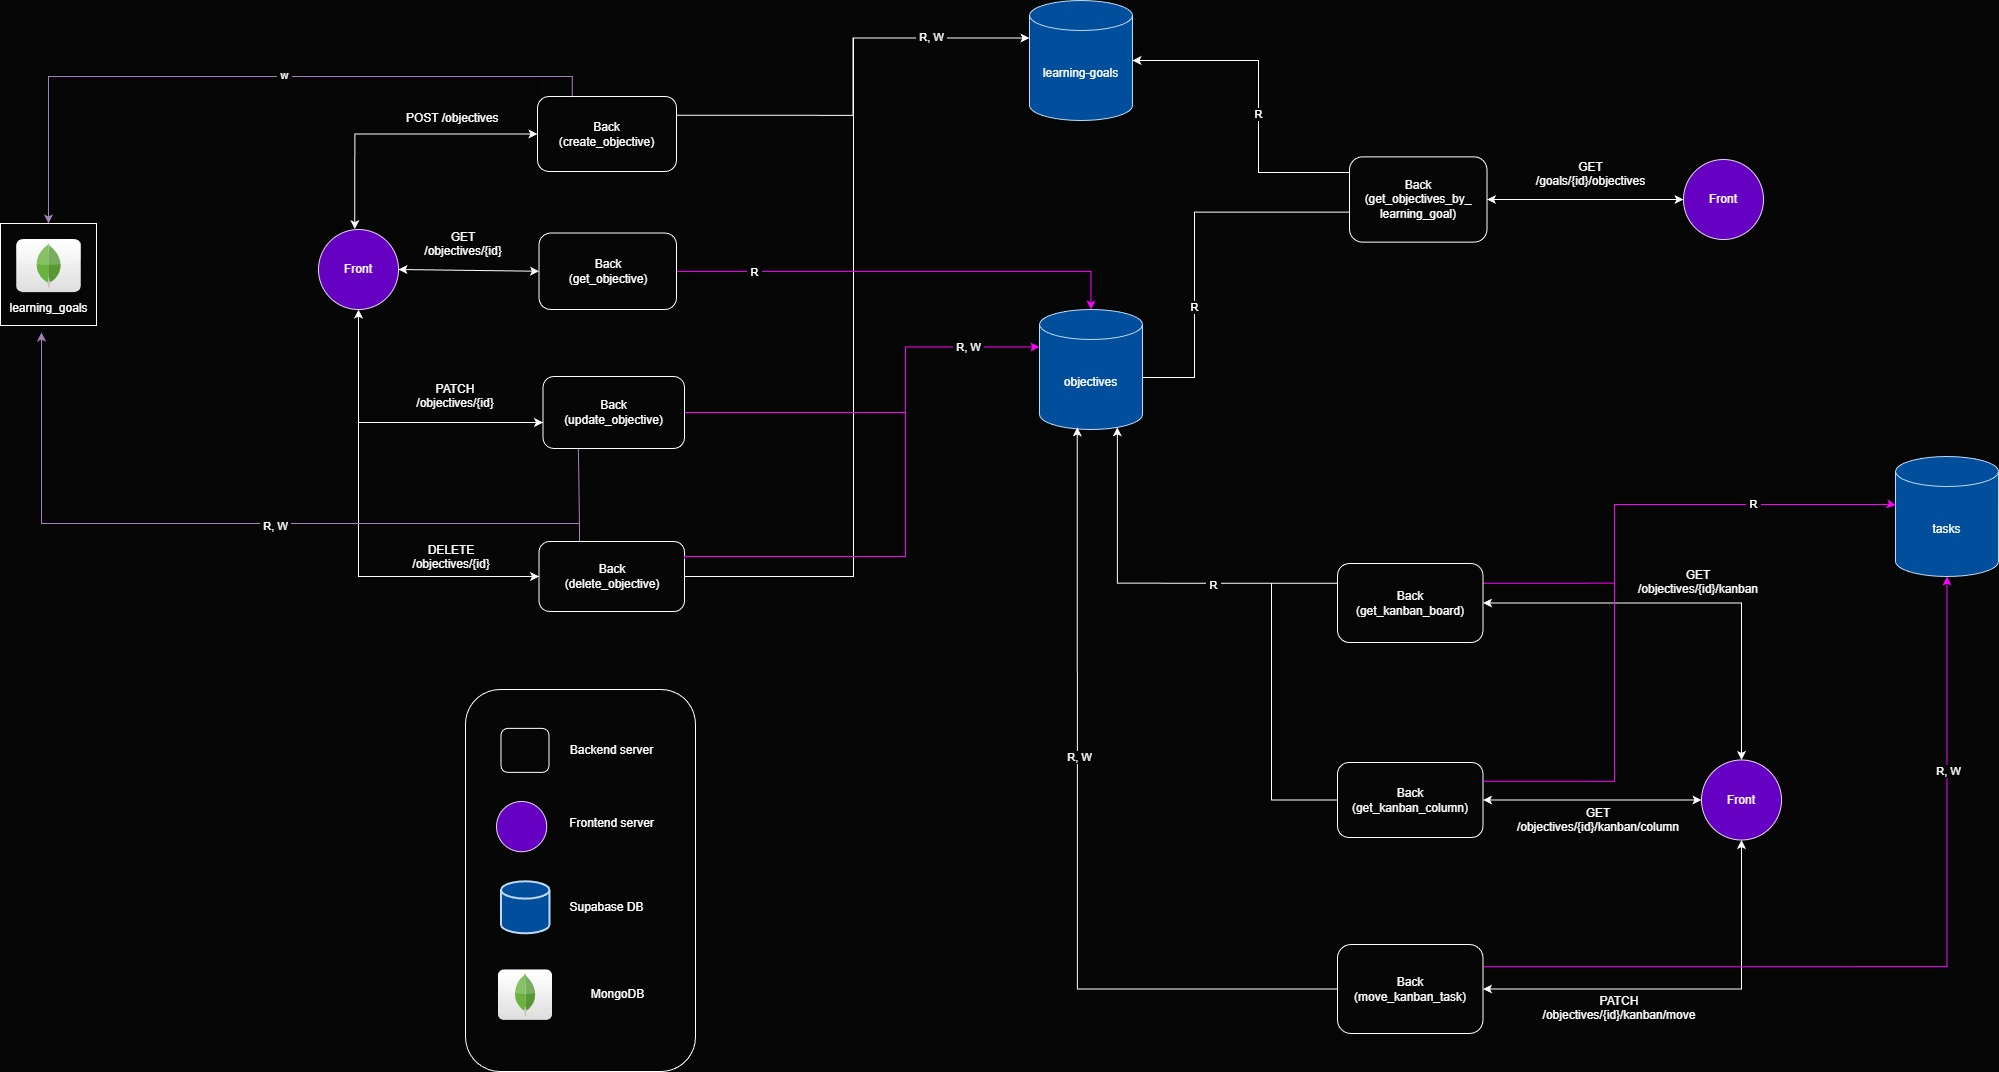
\includegraphics[width=\textwidth]{Figuras/arquitecture_diagrams/objectives.jpg}
\caption{Diagrama de arquitectura para la gestión de objetivos.}
\label{fig:anexoF-objectives}
\end{figure}

% -------------------------------------------------
\subsection*{F.3 Gestión de tareas}
% -------------------------------------------------

\begin{figure}[H]
\centering
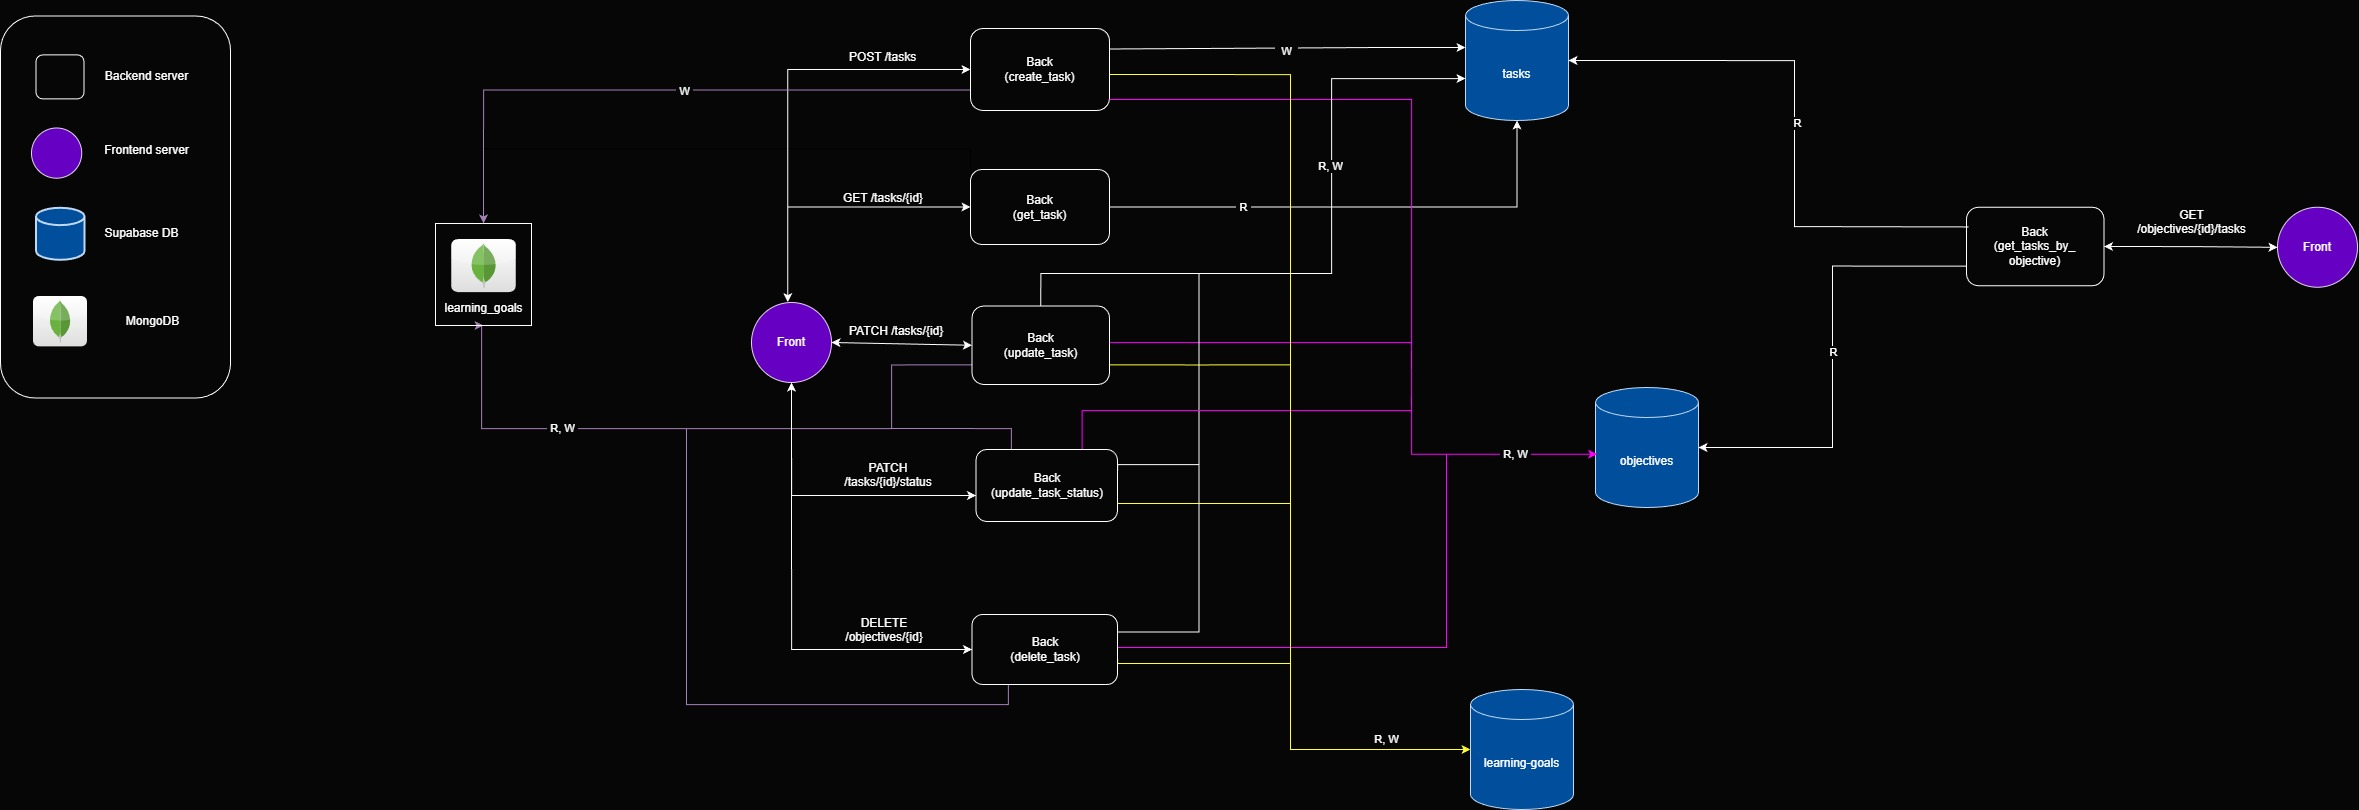
\includegraphics[width=\textwidth]{Figuras/arquitecture_diagrams/tasks.jpg}
\caption{Diagrama de arquitectura para la gestión de tareas.}
\label{fig:anexoF-tasks}
\end{figure}

% -------------------------------------------------
\subsection*{F.4 Notas asociadas a tareas}
% -------------------------------------------------

\begin{figure}[H]
\centering
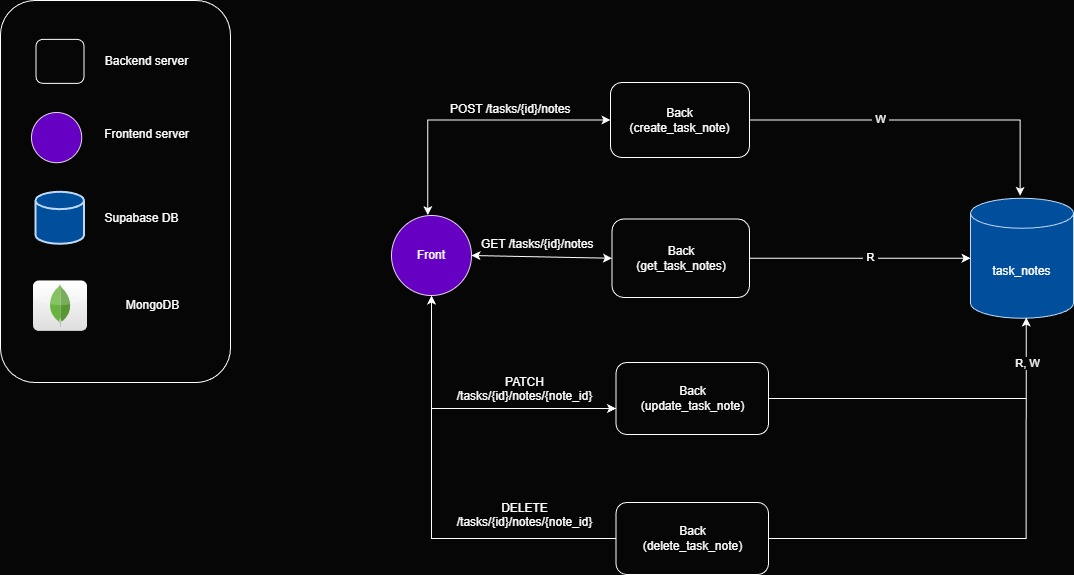
\includegraphics[width=\textwidth]{Figuras/arquitecture_diagrams/task_notes.jpg}
\caption{Diagrama de arquitectura para la gestión de notas asociadas a tareas.}
\label{fig:anexoF-task-notes}
\end{figure}

% -------------------------------------------------
\subsection*{F.5 Recursos asociados a tareas}
% -------------------------------------------------

\begin{figure}[H]
\centering
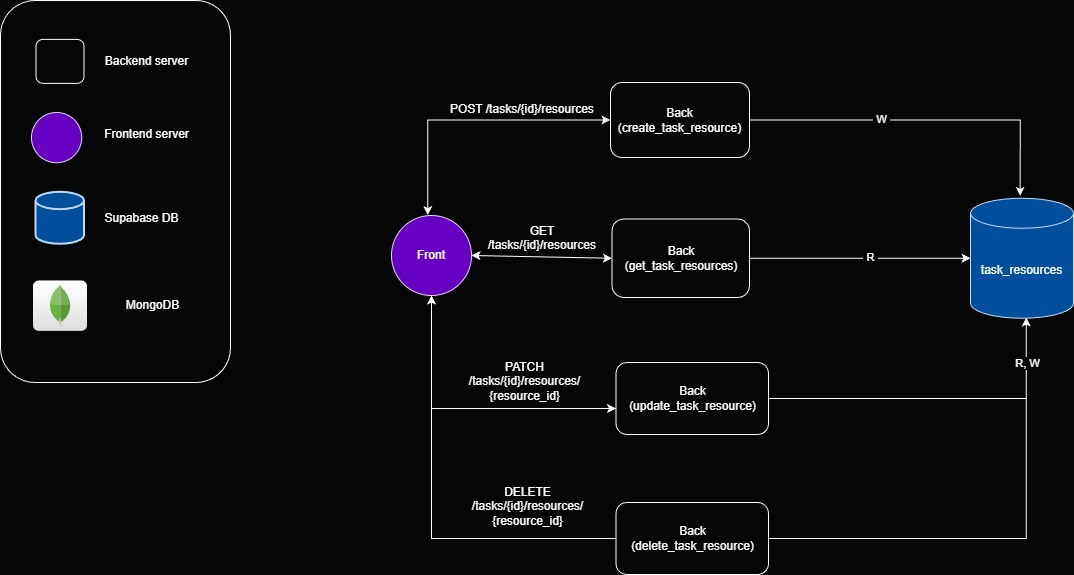
\includegraphics[width=\textwidth]{Figuras/arquitecture_diagrams/task_resources.jpg}
\caption{Diagrama de arquitectura para la gestión de recursos asociados a tareas.}
\label{fig:anexoF-task-resources}
\end{figure}

% -------------------------------------------------
\subsection*{F.6 Autoevaluaciones}
% -------------------------------------------------

\begin{figure}[H]
\centering
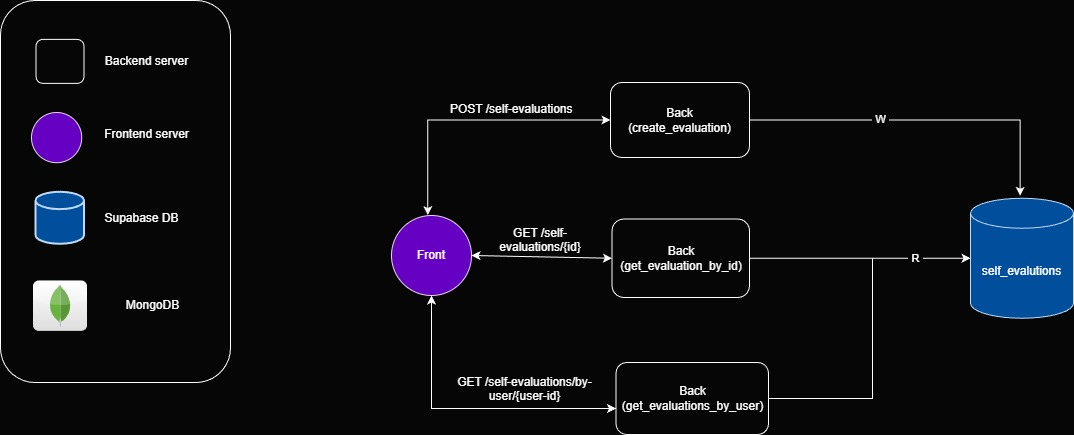
\includegraphics[width=\textwidth]{Figuras/arquitecture_diagrams/self_evaluations.jpg}
\caption{Diagrama de arquitectura para la gestión de autoevaluaciones.}
\label{fig:anexoF-self-evaluations}
\end{figure}

% -------------------------------------------------
\subsection*{F.7 Roadmaps}
% -------------------------------------------------

\begin{figure}[H]
\centering
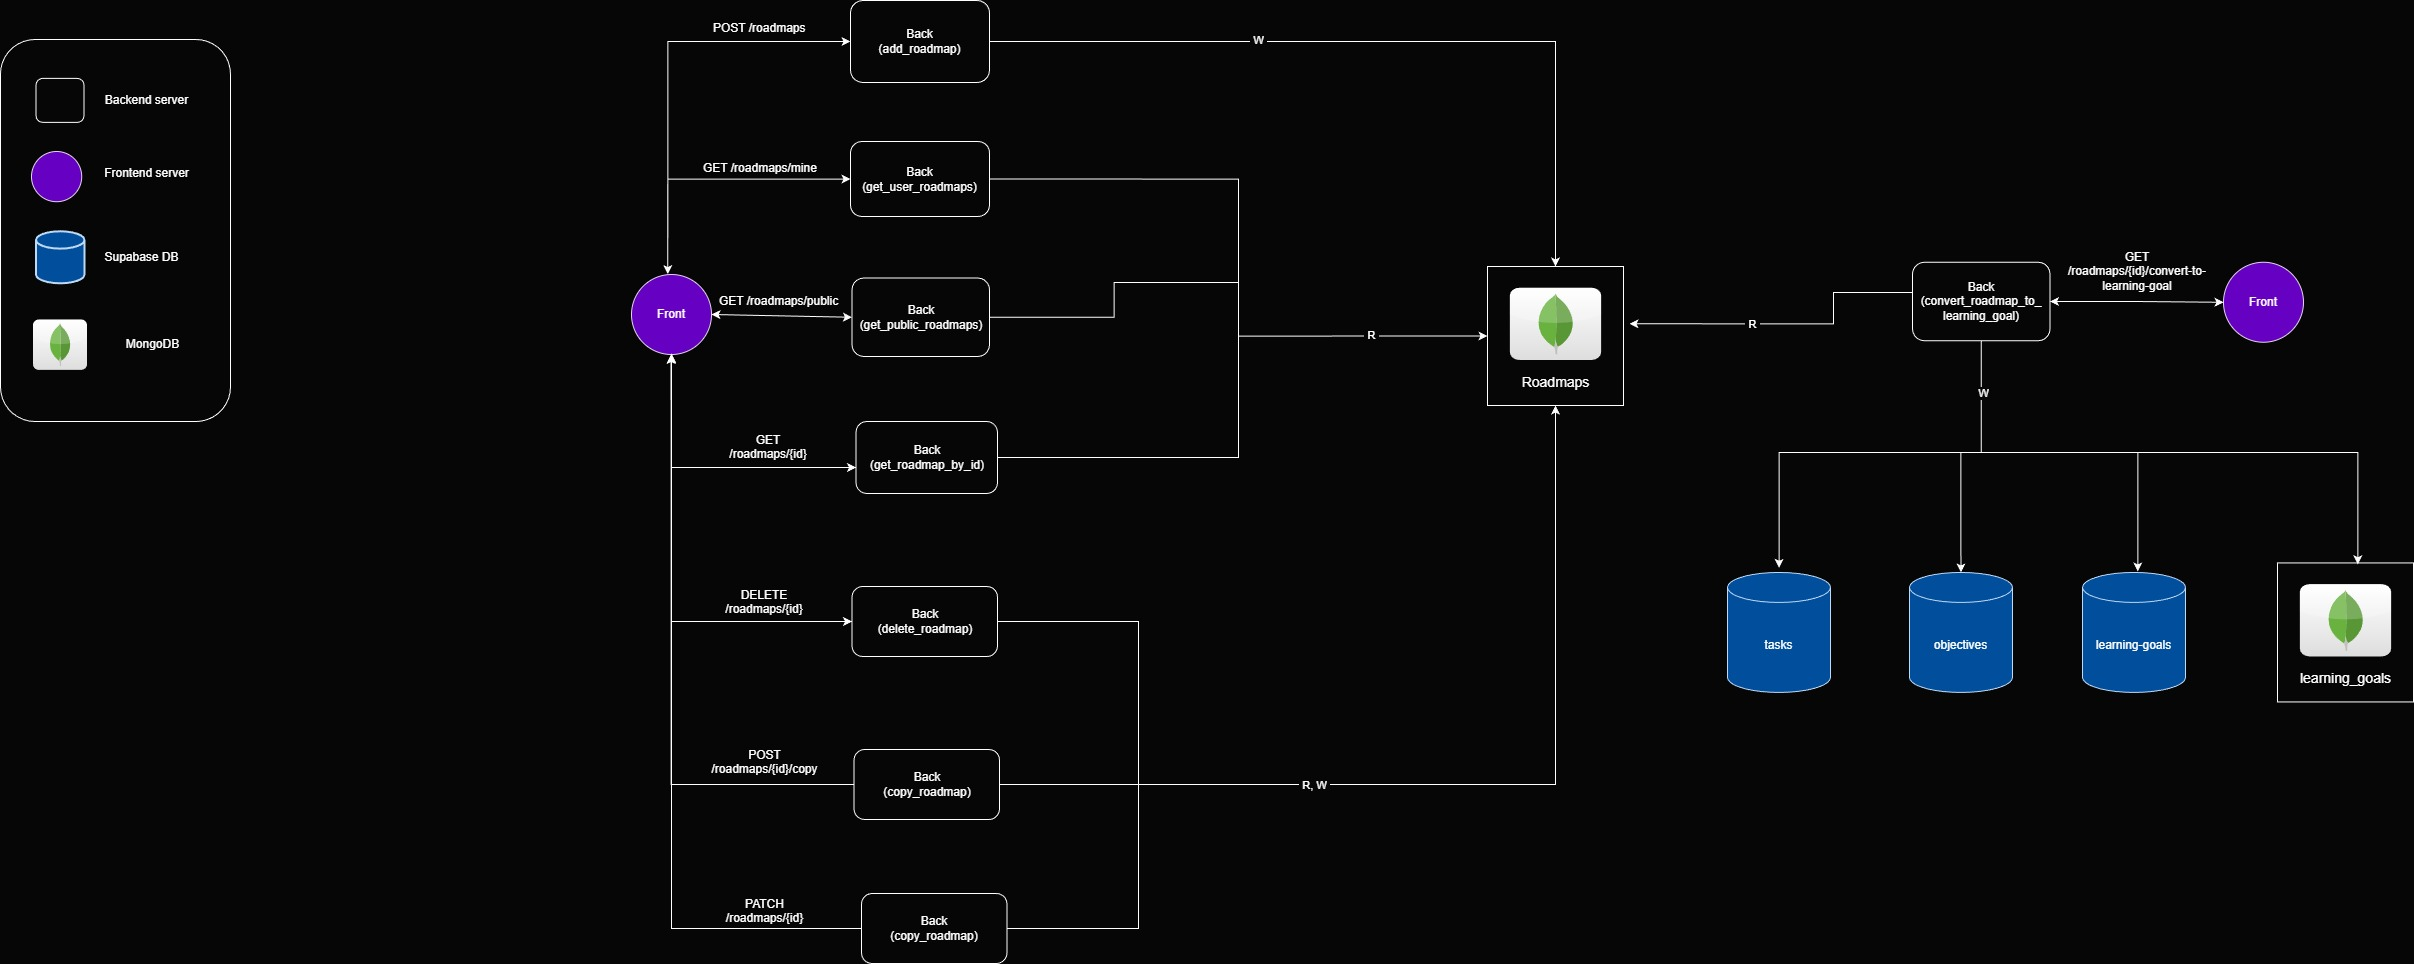
\includegraphics[width=\textwidth]{Figuras/arquitecture_diagrams/roadmaps.jpg}
\caption{Diagrama de arquitectura para la gestión de roadmaps.}
\label{fig:anexoF-roadmaps}
\end{figure}

% -------------------------------------------------
\subsection*{F.8 Sesiones de Escucha Activa}
% -------------------------------------------------

\begin{figure}[H]
\centering
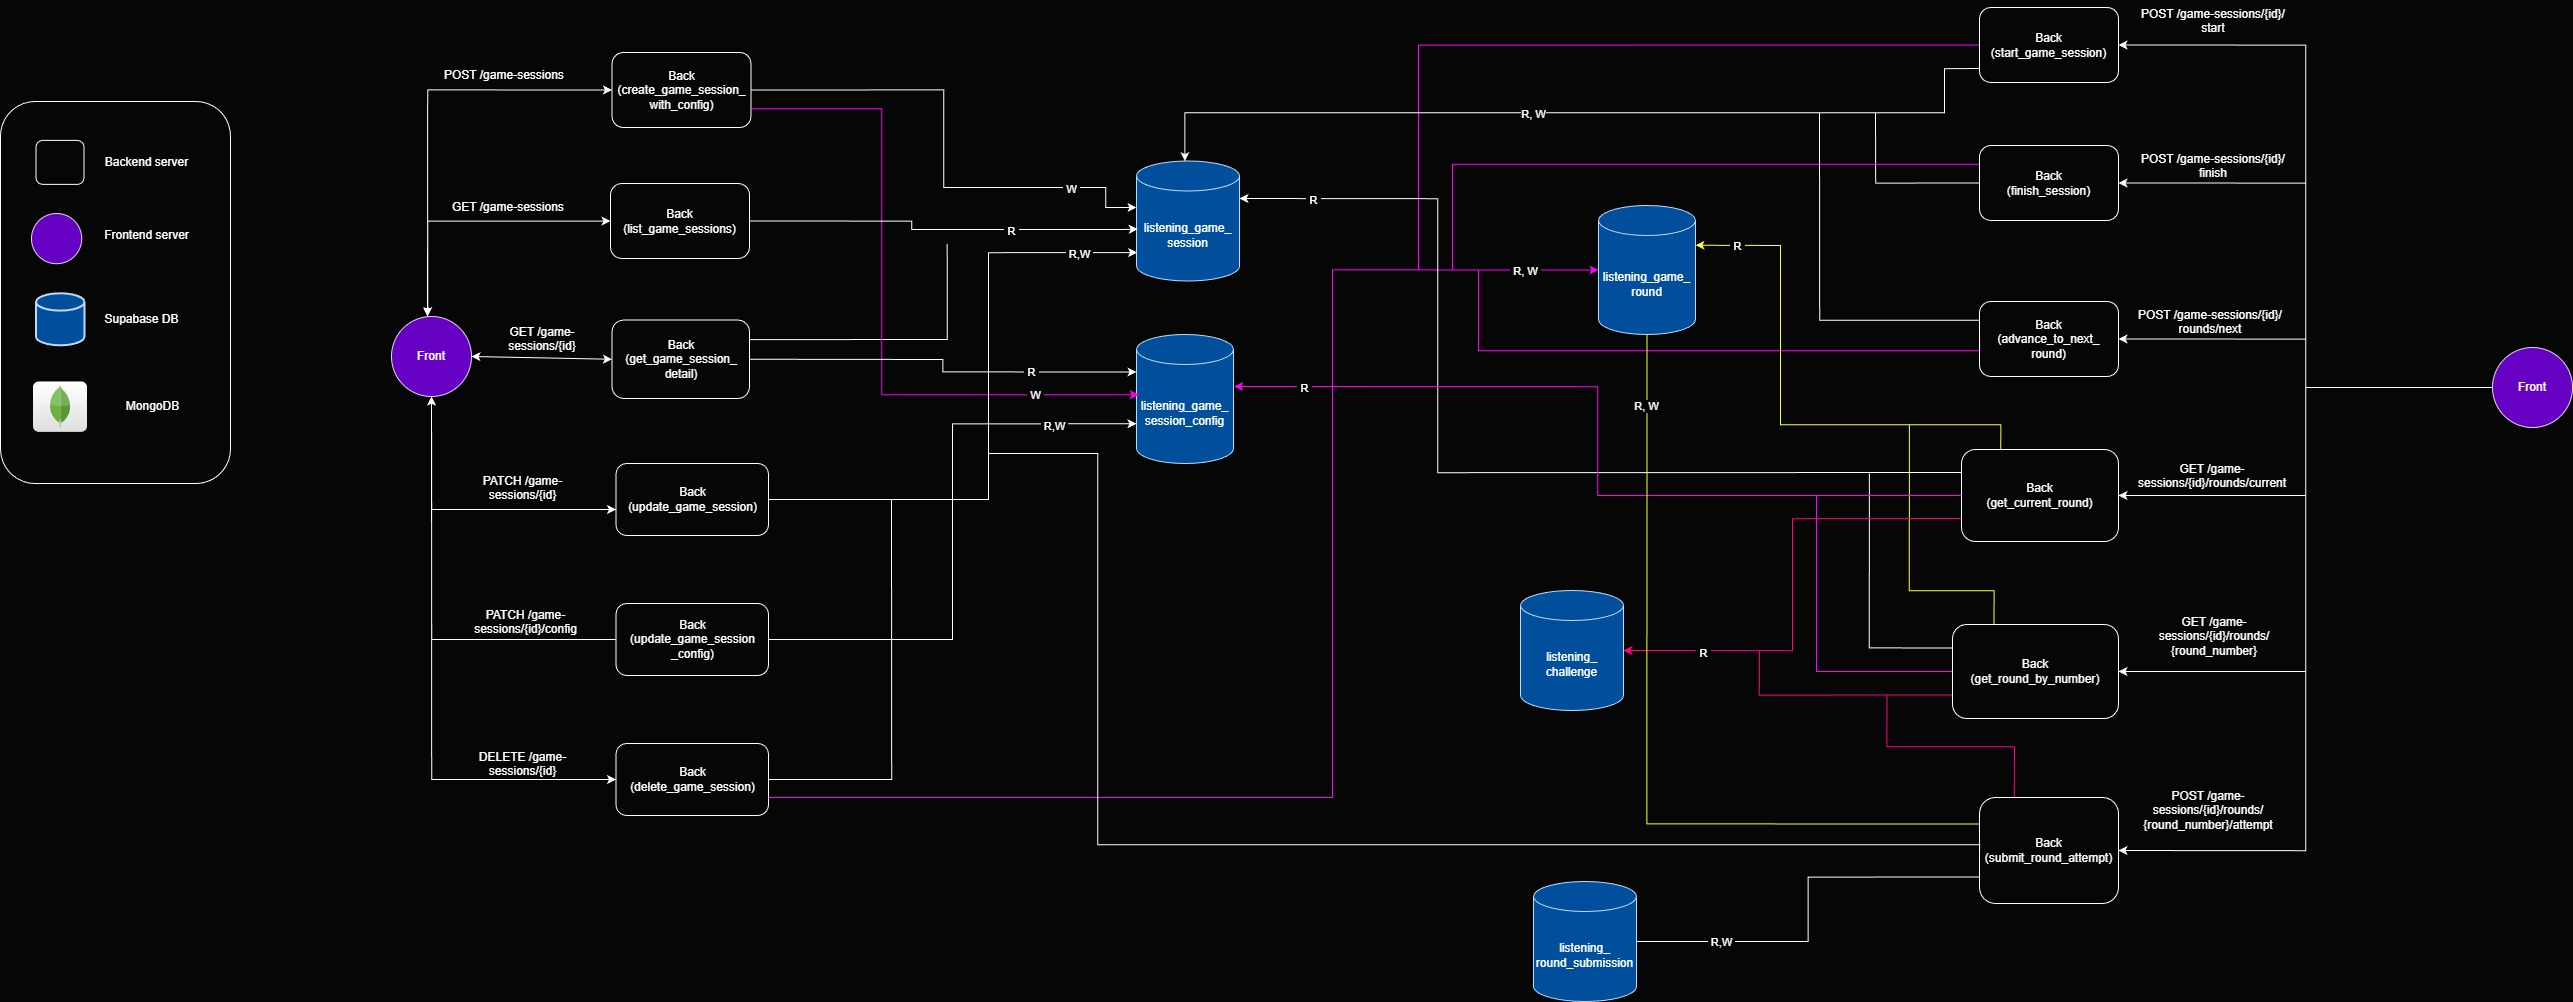
\includegraphics[width=\textwidth]{Figuras/arquitecture_diagrams/game_sessions.jpg}
\caption{Diagrama de arquitectura para las sesiones de Escucha Activa.}
\label{fig:anexoF-listening-sessions}
\end{figure}

% -------------------------------------------------
% Anexo H. Endpoints de la API REST
% -------------------------------------------------
\section*{Anexo H. Especificación detallada de endpoints de la API REST}
\addcontentsline{toc}{section}{Anexo H. Especificación detallada de endpoints de la API REST}
\label{anexo:endpoints}

Esta sección presenta la descripción detallada de los endpoints expuestos por la API REST
del sistema, organizados por dominios funcionales. Para cada grupo se especifican el método
HTTP, la ruta, la acción asociada, una breve descripción, el tipo de autenticación requerida
y el esquema principal de respuesta.

\subsection*{Autenticación y usuarios}

\begin{table}[H]
\centering
\footnotesize
\setlength{\tabcolsep}{4pt}
\renewcommand{\arraystretch}{1.25}
\begin{tabular}{|p{1.4cm}|p{4.1cm}|p{3.2cm}|p{5.8cm}|p{1cm}|}
\hline
\textbf{Método} & \textbf{Ruta} & \textbf{Recurso / acción} & \textbf{Descripción} & \textbf{Auth} \\
\hline

POST & \url{/api/v1/auth/login} & Inicio de sesión &
Autentica al usuario y devuelve un token JWT. &
No \\
\hline

POST & \url{/api/v1/auth/register} & Registro de usuario &
Crea una nueva cuenta de usuario. &
No \\
\hline

PATCH & \url{/api/v1/users/me} & Actualizar perfil &
Actualiza datos del usuario autenticado. &
Sí \\
\hline

DELETE & \url{/api/v1/users/me} & Eliminar cuenta &
Desactiva la cuenta del usuario autenticado. &
Sí \\
\hline

GET & \url{/api/v1/users/me/learning-goals} & Mis metas de aprendizaje &
Obtiene las metas de aprendizaje del usuario con paginación. &
Sí \\
\hline

GET & \url{/api/v1/users/me/pomodoro-preferences} & Obtener preferencias Pomodoro &
Obtiene la configuración de preferencias Pomodoro del usuario. &
Sí \\
\hline

PUT & \url{/api/v1/users/me/pomodoro-preferences} &
Crear/actualizar preferencias Pomodoro &
Crea o actualiza las preferencias Pomodoro del usuario. &
Sí \\
\hline

\end{tabular}
\caption{Endpoints del dominio de autenticación y usuarios.}
\end{table}

% -------------------------------------------------
\subsection*{Módulo Aprender a Aprender}

\subsubsection*{Metas de aprendizaje (\textit{learning\_goals})}

\begin{table}[H]
\centering
\footnotesize
\setlength{\tabcolsep}{4pt}
\renewcommand{\arraystretch}{1.25}
\begin{tabular}{|p{1.4cm}|p{4.1cm}|p{3.2cm}|p{5.8cm}|p{1cm}|}
\hline
\textbf{Método} & \textbf{Ruta} & \textbf{Recurso / acción} & \textbf{Descripción} & \textbf{Auth} \\
\hline

POST & \url{/api/v1/learning-goals} & Crear meta de aprendizaje &
Crea una nueva meta de aprendizaje. &
Sí \\
\hline

GET & \url{/api/v1/learning-goals/{id}} & Obtener meta por ID &
Obtiene los detalles de una meta de aprendizaje. &
Sí \\
\hline

GET & \url{/api/v1/learning-goals/{id}/objectives} & Objetivos de una meta &
Lista los objetivos de una meta con filtros y paginación. &
Sí \\
\hline

PATCH & \url{/api/v1/learning-goals/{id}} & Actualizar meta &
Actualiza los datos de una meta de aprendizaje. &
Sí \\
\hline

DELETE & \url{/api/v1/learning-goals/{id}} & Eliminar meta &
Elimina una meta de aprendizaje. &
Sí \\
\hline

POST & \url{/api/v1/learning-goals/{id}/convert-to-roadmap} & Convertir a roadmap &
Convierte una meta de aprendizaje en un roadmap. &
Sí \\
\hline

\end{tabular}
\caption{Endpoints para la gestión de metas de aprendizaje.}
\end{table}

% -------------------------------------------------
\subsubsection*{Objetivos (\textit{objectives})}

\begin{table}[H]
\centering
\footnotesize
\setlength{\tabcolsep}{4pt}
\renewcommand{\arraystretch}{1.25}
\begin{tabular}{|p{1.4cm}|p{4.1cm}|p{3.2cm}|p{5.8cm}|p{1cm}|}
\hline
\textbf{Método} & \textbf{Ruta} & \textbf{Recurso / acción} & \textbf{Descripción} & \textbf{Auth} \\
\hline

POST & \url{/api/v1/objectives} & Crear objetivo &
Crea un nuevo objetivo de aprendizaje. &
Sí \\
\hline

GET & \url{/api/v1/objectives/{id}} & Obtener objetivo &
Obtiene los detalles de un objetivo. &
Sí \\
\hline

GET & \url{/api/v1/objectives/{id}/tasks} & Tareas de un objetivo &
Lista tareas de un objetivo con filtros y paginación. &
Sí \\
\hline

PATCH & \url{/api/v1/objectives/{id}} & Actualizar objetivo &
Actualiza un objetivo existente. &
Sí \\
\hline

DELETE & \url{/api/v1/objectives/{id}} & Eliminar objetivo &
Elimina un objetivo. &
Sí \\
\hline

GET & \url{/api/v1/objectives/{id}/kanban} & Obtener tablero Kanban &
Obtiene el tablero Kanban de un objetivo. &
Sí \\
\hline

GET & \url{/api/v1/objectives/{id}/kanban/column} & Columna Kanban &
Obtiene tareas paginadas de una columna específica. &
Sí \\
\hline

PATCH & \url{/api/v1/objectives/{id}/kanban/move} & Mover tarea en Kanban &
Mueve una tarea entre columnas del tablero Kanban. &
Sí \\
\hline

\end{tabular}
\caption{Endpoints para la gestión de objetivos.}
\end{table}

% -------------------------------------------------
\subsubsection*{Tareas (\textit{tasks})}

\begin{table}[H]
\centering
\footnotesize
\setlength{\tabcolsep}{4pt}
\renewcommand{\arraystretch}{1.25}
\begin{tabular}{|p{1.4cm}|p{4.1cm}|p{3.2cm}|p{5.8cm}|p{1cm}|}
\hline
\textbf{Método} & \textbf{Ruta} & \textbf{Recurso / acción} & \textbf{Descripción} & \textbf{Auth} \\
\hline

POST & \url{/api/v1/tasks} & Crear tarea &
Crea una nueva tarea asociada a un objetivo. &
Sí \\
\hline

GET & \url{/api/v1/tasks/{id}} & Obtener tarea &
Obtiene los detalles de una tarea. &
Sí \\
\hline

PATCH & \url{/api/v1/tasks/{id}} & Actualizar tarea &
Actualiza los campos de una tarea. &
Sí \\
\hline

PATCH & \url{/api/v1/tasks/{id}/status} & Actualizar estado &
Modifica el estado de una tarea. &
Sí \\
\hline

DELETE & \url{/api/v1/tasks/{id}} & Eliminar tarea &
Elimina una tarea. &
Sí \\
\hline

\end{tabular}
\caption{Endpoints para la gestión de tareas.}
\end{table}

% -------------------------------------------------
\subsubsection*{Notas de tarea (\textit{task\_notes})}

\begin{table}[H]
\centering
\footnotesize
\setlength{\tabcolsep}{4pt}
\renewcommand{\arraystretch}{1.25}
\begin{tabular}{|p{1.4cm}|p{4.1cm}|p{3.2cm}|p{5.8cm}|p{1cm}|}
\hline
\textbf{Método} & \textbf{Ruta} & \textbf{Recurso / acción} & \textbf{Descripción} & \textbf{Auth} \\
\hline

POST & \url{/api/v1/tasks/{task\_id}/notes} & Agregar nota &
Crea una nota asociada a una tarea. &
Sí \\
\hline

GET & \url{/api/v1/tasks/{task\_id}/notes} & Listar notas &
Lista todas las notas de una tarea. &
Sí \\
\hline

PATCH & \url{/api/v1/tasks/{task\_id}/notes/{note\_id}} & Actualizar nota &
Actualiza una nota de tarea. &
Sí \\
\hline

DELETE & \url{/api/v1/tasks/{task\_id}/notes/{note\_id}} & Eliminar nota &
Elimina una nota de tarea. &
Sí \\
\hline

\end{tabular}
\caption{Endpoints para la gestión de notas de tarea.}
\end{table}

% -------------------------------------------------
\subsubsection*{Recursos de tarea (\textit{task\_resources})}

\begin{table}[H]
\centering
\footnotesize
\setlength{\tabcolsep}{4pt}
\renewcommand{\arraystretch}{1.25}
\begin{tabular}{|p{1.4cm}|p{4.1cm}|p{3.2cm}|p{5.8cm}|p{1cm}|}
\hline
\textbf{Método} & \textbf{Ruta} & \textbf{Recurso / acción} & \textbf{Descripción} & \textbf{Auth} \\
\hline

POST & \url{/api/v1/tasks/{task\_id}/resources} & Agregar recurso &
Crea un recurso asociado a una tarea. &
Sí \\
\hline

GET & \url{/api/v1/tasks/{task\_id}/resources} & Listar recursos &
Lista todos los recursos de una tarea. &
Sí \\
\hline

PATCH & \url{/api/v1/tasks/{task\_id}/resources/{resource\_id}} & Actualizar recurso &
Actualiza un recurso de tarea. &
Sí \\
\hline

DELETE & \url{/api/v1/tasks/{task\_id}/resources/{resource\_id}} & Eliminar recurso &
Elimina un recurso de tarea. &
Sí \\
\hline

\end{tabular}
\caption{Endpoints para la gestión de recursos asociados a tareas.}
\end{table}

% -------------------------------------------------
\subsubsection*{Autoevaluaciones (\textit{self\_evaluations})}

\begin{table}[H]
\centering
\footnotesize
\setlength{\tabcolsep}{4pt}
\renewcommand{\arraystretch}{1.25}
\begin{tabular}{|p{1.4cm}|p{4.1cm}|p{3.2cm}|p{5.8cm}|p{1cm}|}
\hline
\textbf{Método} & \textbf{Ruta} & \textbf{Recurso / acción} & \textbf{Descripción} & \textbf{Auth} \\
\hline

POST & \url{/api/v1/self-evaluations} & Crear autoevaluación &
Registra una autoevaluación para una tarea completada. &
Sí \\
\hline

GET & \url{/api/v1/self-evaluations/{evaluation\_id}} & Obtener autoevaluación &
Obtiene una autoevaluación por identificador. &
Sí \\
\hline

GET & \url{/api/v1/self-evaluations/by-user/{user\_id}} & Autoevaluaciones por usuario &
Lista autoevaluaciones de un usuario con filtros y paginación. &
Sí \\
\hline

\end{tabular}
\caption{Endpoints para la gestión de autoevaluaciones.}
\end{table}

% -------------------------------------------------
\subsection*{Módulo Escucha Activa}

\subsubsection*{Sesiones de juego (\textit{game\_sessions})}

\begin{table}[H]
\centering
\footnotesize
\setlength{\tabcolsep}{4pt}
\renewcommand{\arraystretch}{1.25}
\begin{tabular}{|p{1.4cm}|p{4.1cm}|p{3.2cm}|p{5.8cm}|p{1cm}|}
\hline
\textbf{Método} & \textbf{Ruta} & \textbf{Recurso / acción} &
\textbf{Descripción} & \textbf{Auth} \\
\hline

GET & \url{/api/v1/game-sessions} & Listar sesiones &
Lista sesiones de juego del usuario con paginación. &
Sí \\
\hline

POST & \url{/api/v1/game-sessions} & Crear sesión de juego &
Crea una nueva sesión de juego de escucha. &
Sí \\
\hline

POST & \url{/api/v1/game-sessions/{session\_id}/start} & Iniciar sesión &
Inicia una sesión y devuelve la primera ronda. &
Sí \\
\hline

GET & \url{/api/v1/game-sessions/{session\_id}} & Obtener detalles &
Obtiene el detalle de una sesión, incluida su configuración. &
Sí \\
\hline

PATCH & \url{/api/v1/game-sessions/{session\_id}} & Actualizar sesión &
Actualiza nombre y/o estado de la sesión. &
Sí \\
\hline

PATCH & \url{/api/v1/game-sessions/{session\_id}/config} & Actualizar configuración &
Actualiza parcialmente la configuración de la sesión. &
Sí \\
\hline

DELETE & \url{/api/v1/game-sessions/{session\_id}} & Eliminar sesión &
Elimina una sesión de juego. &
Sí \\
\hline

GET & \url{/api/v1/game-sessions/{session\_id}/rounds/current} & Ronda actual &
Obtiene la ronda actual de la sesión. &
Sí \\
\hline

GET & \url{/api/v1/game-sessions/{session\_id}/rounds/{round\_number}} & Ronda específica &
Obtiene una ronda específica por número. &
Sí \\
\hline

POST & \url{/api/v1/game-sessions/{session\_id}/rounds/next} & Siguiente ronda &
Avanza a la siguiente ronda de la sesión. &
Sí \\
\hline

POST & \url{/api/v1/game-sessions/{session\_id}/rounds/{round\_number}/attempt} &
Enviar intento &
Envía un intento de respuesta para una ronda. &
Sí \\
\hline

POST & \url{/api/v1/game-sessions/{session\_id}/rounds/{round\_number}/audio/replay} &
Repetición de audio &
Incrementa el contador de reproducción de audio si está bajo el límite. &
Sí \\
\hline

POST & \url{/api/v1/game-sessions/{session\_id}/finish} & Finalizar sesión &
Marca la sesión como finalizada. &
Sí \\
\hline

GET & \url{/api/v1/game-sessions/{session\_id}/result} & Resultado de sesión &
Obtiene el resultado de una sesión terminada. &
Sí \\
\hline

\end{tabular}
\caption{Endpoints para la gestión de sesiones de juego del módulo Escucha Activa.}
\end{table}

% -------------------------------------------------
\subsubsection*{Desafíos de escucha (\textit{challenges})}

\begin{table}[H]
\centering
\footnotesize
\setlength{\tabcolsep}{4pt}
\renewcommand{\arraystretch}{1.25}
\begin{tabular}{|p{1.4cm}|p{4.1cm}|p{3.2cm}|p{5.8cm}|p{1cm}|}
\hline
\textbf{Método} & \textbf{Ruta} & \textbf{Recurso / acción} &
\textbf{Descripción} & \textbf{Auth} \\
\hline

POST & \url{/api/v1/challenges/generate} & Generar desafío &
Genera un nuevo desafío de escucha usando un modelo LLM. &
No \\
\hline

GET & \url{/api/v1/challenges/{challenge\_id}/audio} & Audio de desafío &
Obtiene o crea el audio asociado a un desafío y devuelve su URL. &
No \\
\hline

\end{tabular}
\caption{Endpoints para la gestión de desafíos de escucha.}
\end{table}

% -------------------------------------------------
\subsection*{Roadmaps (planes de aprendizaje)}

\begin{table}[H]
\centering
\footnotesize
\setlength{\tabcolsep}{4pt}
\renewcommand{\arraystretch}{1.25}
\begin{tabular}{|p{1.4cm}|p{4.1cm}|p{3.2cm}|p{5.8cm}|p{1cm}|}
\hline
\textbf{Método} & \textbf{Ruta} & \textbf{Recurso / acción} &
\textbf{Descripción} & \textbf{Auth} \\
\hline

POST & \url{/api/v1/roadmap} & Crear roadmap &
Crea un nuevo plan de aprendizaje. &
Sí \\
\hline

GET & \url{/api/v1/roadmap/mine} & Mis roadmaps &
Obtiene los planes de aprendizaje del usuario autenticado con paginación. &
Sí \\
\hline

GET & \url{/api/v1/roadmap/public} & Roadmaps públicos &
Lista planes públicos con filtros por título, autor, fechas y número de pasos. &
Sí \\
\hline

GET & \url{/api/v1/roadmap/{id}} & Obtener roadmap &
Obtiene los detalles de un plan de aprendizaje. &
Sí \\
\hline

PATCH & \url{/api/v1/roadmap/{id}} & Actualizar roadmap &
Actualiza la información de un plan de aprendizaje. &
Sí \\
\hline

POST & \url{/api/v1/roadmap/{id}/copy} & Copiar roadmap &
Realiza una copia (clonación) de un plan de aprendizaje. &
Sí \\
\hline

POST & \url{/api/v1/roadmap/{id}/convert-to-learning-goal} & Convertir a meta &
Convierte un roadmap en una meta de aprendizaje accionable. &
Sí \\
\hline

DELETE & \url{/api/v1/roadmap/{id}} & Eliminar roadmap &
Elimina un plan de aprendizaje. &
Sí \\
\hline

\end{tabular}
\caption{Endpoints para la gestión de roadmaps.}
\end{table}

% -------------------------------------------------
\subsection*{Módulos del sistema}

\begin{table}[H]
\centering
\footnotesize
\setlength{\tabcolsep}{4pt}
\renewcommand{\arraystretch}{1.25}
\begin{tabular}{|p{1.4cm}|p{4.1cm}|p{3.2cm}|p{5.8cm}|p{1cm}|}
\hline
\textbf{Método} & \textbf{Ruta} & \textbf{Recurso / acción} &
\textbf{Descripción} & \textbf{Auth} \\
\hline

POST & \url{/api/v1/modules} & Crear módulo &
Crea un nuevo módulo del sistema (requiere rol administrador). &
Sí (admin) \\
\hline

GET & \url{/api/v1/modules} & Listar módulos &
Lista los módulos disponibles con paginación. &
Sí \\
\hline

GET & \url{/api/v1/modules/{id}} & Obtener módulo &
Obtiene los detalles de un módulo. &
Sí \\
\hline

PATCH & \url{/api/v1/modules/{id}} & Actualizar módulo &
Actualiza la información de un módulo (requiere rol administrador). &
Sí (admin) \\
\hline

DELETE & \url{/api/v1/modules/{id}} & Eliminar módulo &
Elimina un módulo del sistema (requiere rol administrador). &
Sí (admin) \\
\hline

\end{tabular}
\caption{Endpoints para la gestión de módulos del sistema.}
\end{table}
% -------------------------------------------------
% Anexo I. Resultados completos de las encuestas aplicadas
% -------------------------------------------------
\section*{Anexo I. Resultados completos de las encuestas aplicadas}
\addcontentsline{toc}{section}{Anexo I. Resultados completos de las encuestas aplicadas}
\label{anexo:encuestas}

El presente anexo reúne la evidencia completa correspondiente a las tres encuestas aplicadas durante la fase de evaluación del prototipo.
\\
\\
Con el fin de mantener el capítulo de resultados enfocado en el análisis, aquí se incluyen los documentos originales generados por Google Forms, así como las tablas completas con los resultados por ítem, promedios y número de respuestas. Cada encuesta aparece organizada según su propósito y población objetivo.

\vspace{0.4cm}

% -------------------------------------------------
% Encuesta 1
% -------------------------------------------------
\subsection*{Encuesta 1: Evaluación del módulo \textit{Aprender a Aprender}}
\addcontentsline{toc}{subsection}{Encuesta 1: Evaluación del módulo Aprender a Aprender}

\vspace{0.2cm}
\noindent\textbf{Archivo anexo:}  
\texttt{Resultados Encuesta 1 - Modulo Aprender a Aprender.pdf}

\vspace{0.5cm}

% ---------- Tablas de la Encuesta 1 ----------
\subsubsection*{Tablas de resultados por ítem}
\addcontentsline{toc}{subsubsection}{Encuesta 1: Tablas de resultados}

% --- Comprensión y uso ---
\begin{table}[H]
\centering
\footnotesize
\setlength{\tabcolsep}{4pt}
\renewcommand{\arraystretch}{1.35}
\begin{tabular}{|p{10.5cm}|c|c|}
\hline
\textbf{Ítem (pregunta literal)} & \textbf{Promedio} & \textbf{N} \\
\hline
Comprendí claramente cómo funcionan las metas de aprendizaje, los objetivos, las tareas y las rutas o planes de aprendizaje dentro del módulo. & 4.32 & 38 \\
\hline
Entendí cómo utilizar el tablero Kanban para organizar y visualizar mis tareas. & 4.26 & 38 \\
\hline
Comprendí cómo usar el chatbot para generar un roadmap de aprendizaje personalizado. & 4.00 & 38 \\
\hline
Entendí el propósito de las autoevaluaciones y reportes de progreso. & 4.39 & 38 \\
\hline
\end{tabular}
\caption{Encuesta 1 – Comprensión y uso de las herramientas del módulo.}
\label{tab:anexo-aaa-comprension}
\end{table}

% --- Motivación y participación ---
\begin{table}[H]
\centering
\footnotesize
\setlength{\tabcolsep}{4pt}
\renewcommand{\arraystretch}{1.35}
\begin{tabular}{|p{10.5cm}|c|c|}
\hline
\textbf{Ítem (pregunta literal)} & \textbf{Promedio} & \textbf{N} \\
\hline
Los procesos de crear metas, objetivos y tareas me mantuvieron participando activamente. & 4.29 & 38 \\
\hline
El tablero Kanban me ayudó a mantenerme activo/a moviendo tareas entre estados. & 4.13 & 38 \\
\hline
El editor visual de roadmaps me permitió involucrarme de forma dinámica con mi plan de aprendizaje. & 4.34 & 38 \\
\hline
La creación de roadmaps con el chatbot fue una experiencia interactiva que me mantuvo comprometido/a. & 4.21 & 38 \\
\hline
El módulo me motivó a trabajar activamente en mis metas de aprendizaje. & 4.29 & 38 \\
\hline
Tener seguimiento visual del progreso (dashboard, porcentajes, estados de tareas) aumentó mi motivación. & 4.42 & 38 \\
\hline
Poder personalizar mis tareas (tipos, recursos, notas) incrementó mi interés en continuar. & 4.39 & 38 \\
\hline
\end{tabular}
\caption{Encuesta 1 – Motivación y participación.}
\label{tab:anexo-aaa-motivacion}
\end{table}

% --- Aplicación práctica ---
\begin{table}[H]
\centering
\footnotesize
\setlength{\tabcolsep}{4pt}
\renewcommand{\arraystretch}{1.35}
\begin{tabular}{|p{10.5cm}|c|c|}
\hline
\textbf{Ítem (pregunta literal)} & \textbf{Promedio} & \textbf{N} \\
\hline
Siento que retuve los conceptos clave sobre planificación, autorregulación y organización del aprendizaje. & 4.32 & 37 \\
\hline
Las autoevaluaciones me ayudaron a recordar mejor mi progreso y aprendizajes. & 4.08 & 37 \\
\hline
El roadmap generado me facilitó recordar los pasos de mi plan de estudio. & 4.38 & 37 \\
\hline
Puedo aplicar en la vida real los conceptos del módulo. & 4.54 & 37 \\
\hline
El roadmap generado me sirve como guía práctica para continuar mi aprendizaje. & 4.27 & 37 \\
\hline
\end{tabular}
\caption{Encuesta 1 – Retención y aplicación práctica.}
\label{tab:anexo-aaa-aplicacion}
\end{table}

% -------------------------------------------------
% Encuesta 2
% -------------------------------------------------
\subsection*{Encuesta 2: Evaluación del módulo \textit{Escucha Activa}}
\addcontentsline{toc}{subsection}{Encuesta 2: Evaluación del módulo Escucha Activa}

\vspace{0.2cm}
\noindent\textbf{Archivo anexo:}  
\texttt{Resultados Encuesta 2 - Modulo Escucha Activa.pdf}

\vspace{0.5cm}

\subsubsection*{Tablas de resultados por ítem}
\addcontentsline{toc}{subsubsection}{Encuesta 2: Tablas de resultados}

% --- Comprensión ---
\begin{table}[H]
\centering
\footnotesize
\setlength{\tabcolsep}{4pt}
\renewcommand{\arraystretch}{1.35}
\begin{tabular}{|p{10.5cm}|c|c|}
\hline
El módulo me ayudó a comprender los principios de la escucha activa y cómo se aplican a situaciones reales. & 4.80 & 25 \\
\hline
Las explicaciones y retroalimentación después de cada ronda fueron claras. & 4.64 & 25 \\
\hline
\end{tabular}
\caption{Encuesta 2 – Comprensión del contenido.}
\label{tab:anexo-ea-comprension}
\end{table}

% --- Motivación ---
\begin{table}[H]
\centering
\footnotesize
\setlength{\tabcolsep}{4pt}
\renewcommand{\arraystretch}{1.35}
\begin{tabular}{|p{10.5cm}|c|c|}
\hline
Las actividades del juego fueron dinámicas y me mantuvieron participando. & 4.72 & 25 \\
\hline
Los distintos modos de juego hicieron la experiencia variada. & 4.48 & 25 \\
\hline
La estructura por rondas, puntajes y feedback me motivó. & 4.52 & 25 \\
\hline
La opción de replay me motivó a mejorar. & 4.44 & 25 \\
\hline
\end{tabular}
\caption{Encuesta 2 – Motivación y participación.}
\label{tab:anexo-ea-motivacion}
\end{table}

% --- Retención ---
\begin{table}[H]
\centering
\footnotesize
\setlength{\tabcolsep}{4pt}
\renewcommand{\arraystretch}{1.35}
\begin{tabular}{|p{10.5cm}|c|c|}
\hline
Siento que mejoré mi capacidad para recordar detalles importantes. & 92\% Sí, 8\% No & 25 \\
\hline
\end{tabular}
\caption{Encuesta 2 – Retención de información (dicotómica).}
\label{tab:anexo-ea-retencion-dicotomica}
\end{table}

\begin{table}[H]
\centering
\footnotesize
\setlength{\tabcolsep}{4pt}
\renewcommand{\arraystretch}{1.35}
\begin{tabular}{|p{10.5cm}|c|c|}
\hline
El uso de diferentes estilos de contenido fortaleció mi comprensión auditiva. & 4.52 & 25 \\
\hline
\end{tabular}
\caption{Encuesta 2 – Retención (Likert).}
\label{tab:anexo-ea-retencion-likert}
\end{table}

% --- Aplicación ---
\begin{table}[H]
\centering
\footnotesize
\setlength{\tabcolsep}{4pt}
\renewcommand{\arraystretch}{1.35}
\begin{tabular}{|p{10.5cm}|c|c|}
\hline
Puedo aplicar técnicas de escucha activa en situaciones reales. & 4.72 & 25 \\
\hline
El proceso del módulo me ayudó a desarrollar habilidades transferibles. & 4.44 & 25 \\
\hline
\end{tabular}
\caption{Encuesta 2 – Aplicación práctica.}
\label{tab:anexo-ea-aplicacion}
\end{table}

% --- Evaluación global ---
\begin{table}[H]
\centering
\footnotesize
\setlength{\tabcolsep}{4pt}
\renewcommand{\arraystretch}{1.35}
\begin{tabular}{|p{10.5cm}|c|c|}
\hline
La experiencia general fue útil, clara y bien diseñada. & 4.84 & 25 \\
\hline
Recomendaría la aplicación a otros estudiantes. & 4.92 & 25 \\
\hline
\end{tabular}
\caption{Encuesta 2 – Evaluación global.}
\label{tab:anexo-ea-global}
\end{table}


\end{document}


